%Page Setup, don't remove
\documentclass[12pt]{book} 
\setlength{\columnsep}{0.7truecm}
\setlength{\parindent}{0cm}
\usepackage[top=2truecm,bottom=2.8truecm, left=2.2truecm, right=2.2truecm,headsep=10pt, paperwidth=19.3truecm, paperheight=27.6truecm]{geometry} 
\usepackage[usenames,dvipsnames,table]{xcolor}
\usepackage{tcolorbox}
\definecolor{ocre}{RGB}{52,177,201} 
\usepackage{pdfpages}
\usepackage{avant}
\usepackage{bussproofs}
\usepackage{mathptmx}
%\usepackage{ebgaramond}
 \usepackage{xeCJK}
 \setCJKmainfont{SimSun}
\usepackage{tikz}
\usepackage{tkz-euclide}
\usepackage{matchsticks}
\usepackage{wrapfig}
\usepackage{listings}
\usepackage[utf8]{vietnam}
\usepackage{babel}
\usepackage[LSBC5,T1]{fontenc}

%----------------------------------------------------------------------------------------
%	VARIOUS REQUIRED PACKAGES
%----------------------------------------------------------------------------------------
\usepackage{titlesec} % Allows customization of titles
\usepackage{multicol}
\usepackage{graphicx} % Required for including pictures
%\graphicspath{{Pictures/}} % Specifies the directory where pictures are stored
\usepackage{lipsum} % Inserts dummy text
\usepackage{tikz} % Required for drawing custom shapes
%\usepackage{enumitem} % Customize lists
%\setlist{nolistsep} % Reduce spacing between bullet points and numbered lists
\usepackage{booktabs} % Required for nicer horizontal rules in tables
\usepackage{eso-pic} % Required for specifying an image background in the title page
\usepackage{titletoc} % Required for manipulating the table of contents
\contentsmargin{0cm} % Removes the default margin
\usepackage{adjustbox} 
\usepackage{amsmath,amsfonts,amssymb,amsthm} % For math equations, theorems, symbols, etc
%\usepackage[framemethod=tikz]{mdframed} 
\usepackage[sexy]{evan}
\usepackage{hyperref}
\urlstyle{same}
\usepackage{tikz} % figure in two column
\usepackage{float}
\usepackage{biblatex}
\usepackage{caption}% dinh dang figure caption
%\usepackage[font=normalsize]{caption}
\usepackage{changepage}
\usepackage{booktabs}

\usepackage{chngcntr}
\usepackage{array}
\usepackage{eurosym}
\usepackage{multirow}
\usepackage{mathtools}
\usepackage{setspace}
\usepackage{afterpage}
\usepackage{scalerel}
\usepackage{blindtext}
\usepackage{tabularx}
\usepackage{afterpage}
\usepackage{array}
%\usepackage{transparent}
\usepackage{efbox}
\usepackage{tabulary}
% \usepackage{CJKutf8}
\usepackage{subcaption}
\usepackage{rotating}
\usepackage{microtype}
\usepackage{pgfplots}

\usetikzlibrary{lindenmayersystems}
\usetikzlibrary{shapes,shapes.geometric}
\usetikzlibrary{decorations.pathreplacing}
\usetikzlibrary{calc,intersections}
\usetikzlibrary[shadings]
\usetikzlibrary{decorations.fractals}

\newmdenv[skipabove=7pt,
skipbelow=7pt,
backgroundcolor=black!5,
linecolor=ocre,
leftline=true,
innerleftmargin=6pt,
innerrightmargin=6pt,
innertopmargin=8pt,
leftmargin=0cm,
rightmargin=0cm,
innerbottommargin=8pt]{tBox}

\def\PIbox#1{\tikz\node[draw = ocre,fill=black!5,align=justify,text width=.95\linewidth,inner sep=2mm]{#1};}%
\renewcommand{\qedsymbol}{}	
\usepackage{fancyhdr} % Required for header and footer configuration
%%%% Header for duong vao toan hoc
\fancypagestyle{duongvaotoanhoc}{
	\fancyhf{}
	\fancyhead[E]{
		\insertpic{63}{740}{1}{duongvao1}
		\insertpic{333}{35}{1}{fduongvao1}
}
	\fancyhead[O]{
		\insertpic{1}{740}{1}{duongvao2}
		\insertpic{59}{34.9}{1}{fduongvao2}
}	
\renewcommand{\footrulewidth}{0pt}
\fancyfoot[LE,RO]{\sffamily\footnotesize	\thepage}

\fancyfoot[LO,RE]{\sffamily\scriptsize TẬP 7 -- SỐ 7--8 THÁNG 8/2023}
}

\fancypagestyle{duongvaotoanhocnone}{
	\fancyhf{}
	\fancyhead[E]{
		\insertpic{333}{35}{1}{fduongvao1}
	}
	\fancyhead[O]{
		\insertpic{59}{34.9}{1}{fduongvao2}
	}	
	\renewcommand{\footrulewidth}{0pt}
	\fancyfoot[LE,RO]{\sffamily\footnotesize	\thepage}
	
	\fancyfoot[LO,RE]{\sffamily\scriptsize TẬP 7 -- SỐ 7--8 THÁNG 8/2023}
}

\fancypagestyle{thachthuctoanhoc}{
	\fancyhf{}
	\fancyhead[E]{
		\insertpic{63}{740}{1}{thachthuc1}
		\insertpic{333}{35}{1}{fthachthuc1}
	}
	\fancyhead[O]{
		\insertpic{1}{740}{1}{thachthuc2}
		\insertpic{59}{34.9}{1}{fthachthuc2}
	}	
	\renewcommand{\footrulewidth}{0pt}
	\fancyfoot[LE,RO]{\sffamily\footnotesize	\thepage}
	
	\fancyfoot[LO,RE]{\sffamily\scriptsize TẬP 7 -- SỐ 7--8 THÁNG 8/2023}
}

\fancypagestyle{thachthuctoanhocnone}{
	\fancyhf{}
	\fancyhead[E]{
		\insertpic{333}{35}{1}{fthachthuc1}
	}
	\fancyhead[O]{
		\insertpic{59}{34.9}{1}{fthachthuc2}
	}	
	\renewcommand{\footrulewidth}{0pt}
	\fancyfoot[LE,RO]{\sffamily\footnotesize	\thepage}
	
	\fancyfoot[LO,RE]{\sffamily\scriptsize TẬP 7 -- SỐ 7--8 THÁNG 8/2023}
}


%%%% Header for Toán học và đời sống
\fancypagestyle{toanhocvadoisong}{
			\fancyhf{}
		\fancyhead[E]{
			\insertpic{63}{740}{1}{toanhocds1}
			\insertpic{333}{35}{1}{ftoanhocds1}
		}
		\fancyhead[O]{
			\insertpic{1}{740}{1}{toanhocds2}
			\insertpic{59}{34.9}{1}{ftoanhocds2}
		}	
		\renewcommand{\footrulewidth}{0pt}
		\fancyfoot[LE,RO]{\sffamily\footnotesize	\thepage}
		
		\fancyfoot[LO,RE]{\sffamily\scriptsize TẬP 7 -- SỐ 7--8 THÁNG 8/2023}
}
\fancypagestyle{toanhocvadoisongnone}{
	\fancyhf{}
	\fancyhead[E]{
		\insertpic{333}{35}{1}{ftoanhocds1}
	}
	\fancyhead[O]{
		\insertpic{59}{34.9}{1}{ftoanhocds2}
	}	
	\renewcommand{\footrulewidth}{0pt}
	\fancyfoot[LE,RO]{\sffamily\footnotesize	\thepage}
	
	\fancyfoot[LO,RE]{\sffamily\scriptsize TẬP 7 -- SỐ 7--8 THÁNG 8/2023}
}

\fancypagestyle{doisongtoanhoc}{
	\fancyhf{}
	\fancyhead[E]{
		\insertpic{63}{740}{1}{dstoanhoc1}
		\insertpic{333}{35}{1}{fdstoanhoc1}
	}
	\fancyhead[O]{
		\insertpic{1}{740}{1}{dstoanhoc2}
		\insertpic{59}{34.9}{1}{fdstoanhoc2}
	}	
	\renewcommand{\footrulewidth}{0pt}
	\fancyfoot[LE,RO]{\sffamily\footnotesize	\thepage}
	
	\fancyfoot[LO,RE]{\sffamily\scriptsize TẬP 7 -- SỐ 7--8 THÁNG 8/2023}
}
\fancypagestyle{doisongtoanhocnone}{
	\fancyhf{}
	\fancyhead[E]{
		\insertpic{333}{35}{1}{fdstoanhoc1}
	}
	\fancyhead[O]{
		\insertpic{59}{34.9}{1}{fdstoanhoc2}
	}	
	\renewcommand{\footrulewidth}{0pt}
	\fancyfoot[LE,RO]{\sffamily\footnotesize	\thepage}
	
	\fancyfoot[LO,RE]{\sffamily\scriptsize TẬP 7 -- SỐ 7--8 THÁNG 8/2023}
}

%%% doi thoai toan hoc
\fancypagestyle{doithoaitoanhoc}{
	\fancyhf{}
	\fancyhead[E]{
		\insertpic{63}{740}{1}{doithoai1}
		\insertpic{333}{35}{1}{fdoithoai1}
	}
	\fancyhead[O]{
		\insertpic{1}{740}{1}{doithoai2}
		\insertpic{59}{34.9}{1}{fdoithoai2}
	}	
	\renewcommand{\footrulewidth}{0pt}
	\fancyfoot[LE,RO]{\sffamily\footnotesize	\thepage}
	
	\fancyfoot[LO,RE]{\sffamily\scriptsize TẬP 7 -- SỐ 7--8 THÁNG 8/2023}
}
\fancypagestyle{doithoaitoanhocnone}{
	\fancyhf{}
	\fancyhead[E]{
		\insertpic{333}{35}{1}{fdoithoai1}
	}
	\fancyhead[O]{
		\insertpic{59}{34.9}{1}{fdoithoai2}
	}	
	\renewcommand{\footrulewidth}{0pt}
	\fancyfoot[LE,RO]{\sffamily\footnotesize	\thepage}
	
	\fancyfoot[LO,RE]{\sffamily\scriptsize TẬP 7 -- SỐ 7--8 THÁNG 8/2023}
}

%%%% Header for co dien hien dai
\fancypagestyle{codienhiendai}{
	\fancyhf{}
	\fancyhead[E]{
		\insertpic{63}{740}{1}{codien1}
		\insertpic{333}{35}{1}{fcodien1}
	}
	\fancyhead[O]{
		\insertpic{1}{740}{1}{codien2}
		\insertpic{59}{34.9}{1}{fcodien2}
	}	
	\renewcommand{\footrulewidth}{0pt}
	\fancyfoot[LE,RO]{\sffamily\footnotesize	\thepage}
	
	\fancyfoot[LO,RE]{\sffamily\scriptsize TẬP 7 -- SỐ 7--8 THÁNG 8/2023}
}
\fancypagestyle{codienhiendainone}{
	\fancyhf{}
	\fancyhead[E]{
		\insertpic{333}{35}{1}{fcodien1}
	}
	\fancyhead[O]{
		\insertpic{59}{34.9}{1}{fcodien2}
	}	
	\renewcommand{\footrulewidth}{0pt}
	\fancyfoot[LE,RO]{\sffamily\footnotesize	\thepage}
	
	\fancyfoot[LO,RE]{\sffamily\scriptsize TẬP 7 -- SỐ 7--8 THÁNG 8/2023}
}

\fancypagestyle{diendandayvahoctoan}{
	\fancyhf{}
	\fancyhead[E]{
		\insertpic{63}{740}{1}{diendan1}
		\insertpic{333}{35}{1}{fdiendan1}
	}
	\fancyhead[O]{
		\insertpic{1}{740}{1}{diendan2}
		\insertpic{59}{34.9}{1}{fdiendan2}
	}	
	\renewcommand{\footrulewidth}{0pt}
	\fancyfoot[LE,RO]{\sffamily\footnotesize	\thepage}
	
	\fancyfoot[LO,RE]{\sffamily\scriptsize TẬP 7 -- SỐ 7--8 THÁNG 8/2023}
}
\fancypagestyle{diendandayvahoctoannone}{
	\fancyhf{}
	\fancyhead[E]{
		\insertpic{333}{35}{1}{fdiendan1}
	}
	\fancyhead[O]{
		\insertpic{59}{34.9}{1}{fdiendan2}
	}	
	\renewcommand{\footrulewidth}{0pt}
	\fancyfoot[LE,RO]{\sffamily\footnotesize	\thepage}
	
	\fancyfoot[LO,RE]{\sffamily\scriptsize TẬP 7 -- SỐ 7--8 THÁNG 8/2023}
}

\fancypagestyle{cackithitoan}{
	\fancyhf{}
	\fancyhead[E]{
		\insertpic{63}{740}{1}{cackithi1}
		\insertpic{333}{35}{1}{fcackithi1}
	}
	\fancyhead[O]{
		\insertpic{1}{740}{1}{cackithi2}
		\insertpic{59}{34.9}{1}{fcackithi2}
	}	
	\renewcommand{\footrulewidth}{0pt}
	\fancyfoot[LE,RO]{\sffamily\footnotesize	\thepage}
	
	\fancyfoot[LO,RE]{\sffamily\scriptsize TẬP 7 -- SỐ 7--8 THÁNG 8/2023}
}
\fancypagestyle{cackithitoannone}{
	\fancyhf{}
	\fancyhead[E]{
		\insertpic{333}{35}{1}{fcackithi1}
	}
	\fancyhead[O]{
		\insertpic{59}{34.9}{1}{fcackithi2}
	}	
	\renewcommand{\footrulewidth}{0pt}
	\fancyfoot[LE,RO]{\sffamily\footnotesize	\thepage}
	
	\fancyfoot[LO,RE]{\sffamily\scriptsize TẬP 7 -- SỐ 7--8 THÁNG 8/2023}
}

\fancypagestyle{lichsutoanhoc}{
	\fancyhf{}
	\fancyhead[E]{
		\insertpic{63}{740}{1}{lichsu1}
		\insertpic{333}{35}{1}{flichsu1}
	}
	\fancyhead[O]{
		\insertpic{1}{740}{1}{lichsu2}
		\insertpic{59}{34.9}{1}{flichsu2}
	}	
	\renewcommand{\footrulewidth}{0pt}
	\fancyfoot[LE,RO]{\sffamily\footnotesize	\thepage}
	
	\fancyfoot[LO,RE]{\sffamily\scriptsize TẬP 7 -- SỐ 7--8 THÁNG 8/2023}
}
\fancypagestyle{lichsutoanhocnone}{
	\fancyhf{}
	\fancyhead[E]{
		\insertpic{333}{35}{1}{flichsu1}
	}
	\fancyhead[O]{
		\insertpic{59}{34.9}{1}{flichsu2}
	}	
	\renewcommand{\footrulewidth}{0pt}
	\fancyfoot[LE,RO]{\sffamily\footnotesize	\thepage}
	
	\fancyfoot[LO,RE]{\sffamily\scriptsize TẬP 7 -- SỐ 7--8 THÁNG 8/2023}
}

%%%% Header for Tìm hiểu khoa học
\fancypagestyle{timhieukhoahoc}{
		\fancyhf{}
	\fancyhead[E]{
		\insertpic{63}{740}{1}{timhieu1}
		\insertpic{333}{35}{1}{ftimhieu1}
	}
	\fancyhead[O]{
		\insertpic{1}{740}{1}{timhieu2}
		\insertpic{59}{34.9}{1}{ftimhieu2}
	}	
	\renewcommand{\footrulewidth}{0pt}
	\fancyfoot[LE,RO]{\sffamily\footnotesize	\thepage}
	
	\fancyfoot[LO,RE]{\sffamily\scriptsize TẬP 7 -- SỐ 7--8 THÁNG 8/2023}	
}
\fancypagestyle{timhieukhoahocnone}{
	\fancyhf{}
	\fancyhead[E]{
		\insertpic{333}{35}{1}{ftimhieu1}
	}
	\fancyhead[O]{
		\insertpic{59}{34.9}{1}{ftimhieu2}
	}	
	\renewcommand{\footrulewidth}{0pt}
	\fancyfoot[LE,RO]{\sffamily\footnotesize	\thepage}
	
	\fancyfoot[LO,RE]{\sffamily\scriptsize TẬP 7 -- SỐ 7--8 THÁNG 8/2023}	
}

%%%% Header for quan toan
\fancypagestyle{quantoan}{
		\fancyhf{}
		\fancyhead[E]{
		\insertpic{63}{740}{1}{quantoan1}
		\insertpic{333}{35}{1}{fquantoan1}
	}
	\fancyhead[O]{
		\insertpic{1}{740}{1}{quantoan2}
		\insertpic{59}{34.9}{1}{fquantoan2}
	}	
	\renewcommand{\footrulewidth}{0pt}
	\fancyfoot[LE,RO]{\sffamily\footnotesize	\thepage}
	
	\fancyfoot[LO,RE]{\sffamily\scriptsize TẬP 7 -- SỐ 7--8 THÁNG 8/2023}
}
\fancypagestyle{quantoannone}{
	\fancyhf{}
	\fancyhead[E]{
		\insertpic{333}{35}{1}{fquantoan1}
	}
	\fancyhead[O]{
		\insertpic{59}{34.9}{1}{fquantoan2}
	}	
	\renewcommand{\footrulewidth}{0pt}
	\fancyfoot[LE,RO]{\sffamily\footnotesize	\thepage}
	
	\fancyfoot[LO,RE]{\sffamily\scriptsize TẬP 7 -- SỐ 7--8 THÁNG 8/2023}
}


\fancypagestyle{hoccungpi}{
				\fancyhf{}
		\fancyhead[E]{
			\insertpic{63}{740}{1}{hoccungpi1}
			\insertpic{333}{35}{1}{fhoccungpi1}
		}
		\fancyhead[O]{
			\insertpic{1}{740}{1}{hoccungpi2}
			\insertpic{59}{34.9}{1}{fhoccungpi2}
		}	
		\renewcommand{\footrulewidth}{0pt}
		\fancyfoot[LE,RO]{\sffamily\footnotesize	\thepage}
		
		\fancyfoot[LO,RE]{\sffamily\scriptsize TẬP 7 -- SỐ 7--8 THÁNG 8/2023}	
}
\fancypagestyle{hoccungpinone}{
	\fancyhf{}
	\fancyhead[E]{
		\insertpic{333}{35}{1}{fhoccungpi1}
	}
	\fancyhead[O]{
		\insertpic{59}{34.9}{1}{fhoccungpi2}
	}	
	\renewcommand{\footrulewidth}{0pt}
	\fancyfoot[LE,RO]{\sffamily\footnotesize	\thepage}
	
	\fancyfoot[LO,RE]{\sffamily\scriptsize TẬP 7 -- SỐ 7--8 THÁNG 8/2023}	
}

\fancypagestyle{toancuabi}{
	\fancyhf{}
	\fancyhead[E]{
		\insertpic{63}{740}{1}{toancuabi1}
		\insertpic{333}{35}{1}{ftoancuabi1}
	}
	\fancyhead[O]{
		\insertpic{1}{740}{1}{toancuabi2}
		\insertpic{59}{34.9}{1}{ftoancuabi2}
	}	
	\renewcommand{\footrulewidth}{0pt}
	\fancyfoot[LE,RO]{\sffamily\footnotesize	\thepage}
	
	\fancyfoot[LO,RE]{\sffamily\scriptsize TẬP 7 -- SỐ 7--8 THÁNG 8/2023}	
}
\fancypagestyle{toancuabinone}{
	\fancyhf{}
	\fancyhead[E]{
		\insertpic{333}{35}{1}{ftoancuabi1}
	}
	\fancyhead[O]{
		\insertpic{59}{34.9}{1}{ftoancuabi2}
	}	
	\renewcommand{\footrulewidth}{0pt}
	\fancyfoot[LE,RO]{\sffamily\footnotesize	\thepage}
	
	\fancyfoot[LO,RE]{\sffamily\scriptsize TẬP 7 -- SỐ 7--8 THÁNG 8/2023}	
}

\fancypagestyle{gocco}{
	\fancyhf{}
	\fancyhead[E]{
		\insertpic{63}{740}{1}{gocco1}
		\insertpic{333}{35}{1}{fgocco1}
	}
	\fancyhead[O]{
		\insertpic{1}{740}{1}{gocco2}
		\insertpic{59}{34.9}{1}{fgocco2}
	}	
	\renewcommand{\footrulewidth}{0pt}
	\fancyfoot[LE,RO]{\sffamily\footnotesize	\thepage}
	
	\fancyfoot[LO,RE]{\sffamily\scriptsize TẬP 7 -- SỐ 7--8 THÁNG 8/2023}	
}

\fancypagestyle{gocconone}{
	\fancyhf{}
	\fancyhead[E]{
		\insertpic{333}{35}{1}{fgocco1}
	}
	\fancyhead[O]{
		\insertpic{59}{34.9}{1}{fgocco2}
	}	
	\renewcommand{\footrulewidth}{0pt}
	\fancyfoot[LE,RO]{\sffamily\footnotesize	\thepage}
	
	\fancyfoot[LO,RE]{\sffamily\scriptsize TẬP 7 -- SỐ 7--8 THÁNG 8/2023}	
}
	
%	\fancyfoot[C]{\sffamily\footnotesize Tạp chí Pi } % Print the nearest section name on the left side of odd pages	


\pagestyle{fancy}
\renewcommand{\chaptermark}[1]{\markboth{\normalsize\bfseries\chaptername\ \thechapter.\ #1}{}} % Chapter text font settings
\renewcommand{\sectionmark}[1]{\markright{\normalsize\thesection\hspace{5pt}#1}{}} % Section text font settings


\fancyfoot[LE,RO]{\sffamily\footnotesize	\thepage} % Font setting for the page number in the header
\fancyfoot[LO,RE]{\sffamily\footnotesize TẬP 7 -- SỐ 7--8 THÁNG 8/2023 \LARGE  $\pmb{\pi}$}


\fancyfoot[C]{\sffamily\footnotesize Tạp chí Pi } % Print the nearest section name on the left side of odd pages
\renewcommand{\headrulewidth}{0pt} % Width of the rule under the header
\addtolength{\headheight}{2.5pt} % Increase the spacing around the header slightly
\renewcommand{\footrulewidth}{.5pt} % Removes the rule in the footer


\fancypagestyle{plain}{\fancyhead{}\renewcommand{\headrulewidth}{0pt}} % Style for when a plain pagestyle is specified

% Removes the header from odd empty pages at the end of chapters
\makeatletter
\renewcommand{\cleardoublepage}{
	\clearpage\ifodd\c@page\else
	\hbox{}
	\vspace*{\fill}
	\thispagestyle{empty}
	\newpage
	\fi}


\graphicspath{{../main/pic/}}
\everymath{\displaystyle}
\DeclareMathAlphabet{\pazocal}{OMS}{zplm}{m}{n}
\usepackage{ebgaramond}
\usepackage{xpatch}
\PassOptionsToPackage{hyphens}{url}

\usepackage{url}
\usepackage{type1cm}
\usepackage{lettrine}
\usepackage{makecell}
\renewcommand{\LettrineTextFont}{\rmfamily}
\usepackage{skak}
%\usepackage{xskak}
\usepackage{tabularx}

\usepackage{microtype}
\usepackage{cases}
\usepackage{tikz-cd}
\usepackage{oplotsymbl}

\definecolor{codienhiendai}{cmyk}{0.72, 0, 0.42, 0.1}
\definecolor{thachthuctoanhoc}{cmyk}{0.87, 0.46, 0.69, 0.31}
\definecolor{diendantoanhoc}{cmyk}{0.75, 0, 0.7, 0}
\definecolor{timhieukhoahoc}{cmyk}{0.84, 0.7, 0, 0}
\definecolor{quantoan}{cmyk}{0.8, 0.57, 0, 0}
\definecolor{cackithi}{cmyk}{0.7, 0.35, 0, 0}
\definecolor{hoccungpi}{cmyk}{0.67, 0.6, 0, 0}
\definecolor{gocco}{cmyk}{0.65, 0.78, 0, 0}
\definecolor{toancuabi}{cmyk}{0, 1, 0, 0}
\definecolor{doithoaitoanhoc}{cmyk}{0.6, 0.3, 0 ,0.63}
\definecolor{duongvaotoanhoc}{cmyk}{0, 0.7, 0.9, 0}
\definecolor{toanhocdoisong}{cmyk}{0 , 0.93, 1, 0}
\definecolor{tramthienvan}{cmyk}{0, 0.98, 0.95, 0}
\definecolor{lichsutoanhoc}{cmyk}{0.35, 0.5, 0.8, 0.1}
\definecolor{doisongtoanhoc}{cmyk}{0.25, 0.3, 0.5, 0.1}
\definecolor{amber}{rgb}{1.0, 0.75, 0.0}

\definecolor{darkblue}{rgb}{0.089,0.21,0.363}
\usepackage[hang,splitrule]{footmisc}
\usetikzlibrary{arrows}
\usetikzlibrary{patterns}
\usetikzlibrary{decorations.pathreplacing,calligraphy,backgrounds}
\setlength{\footnotemargin}{0cm}
\setlength{\footnotesep}{0.35cm}
\setlength{\skip\footins}{0.35cm}
\setlength\footskip{33pt}

\newcommand\blfootnote[1]{%
	\begingroup
	\renewcommand\thefootnote{}\footnote{#1}%
	\addtocounter{footnote}{-1}%
	\endgroup
}

\def\footnotelayout{\itshape}
\renewcommand*\footnoterule{}
\renewcommand\footnoterule{\vspace*{0.25cm}\hrule width 1\textwidth\vspace*{0.25cm}}

\newcommand{\insertpic}[4]{
	\begingroup
	\AddToShipoutPicture*{\put(#1,#2){\includegraphics[scale=#3]{#4}}} % %Image background
	\centering
	\endgroup
}

\tikzset{
	squarednode/.style={rectangle, draw=red!60, fill=red!5, very thick, minimum size=3mm}
}

\tikzset{
	sqnode/.style={rectangle, draw=cackithi, very thick, minimum size=3mm}
}

\tikzset{
	roundnode/.style={circle, draw=toancuabi, fill=cackithi!50, minimum size=3mm},
}


\begin{document}
%	 \thispagestyle{empty}
%	 \begingroup 
%	 \AddToShipoutPicture*{\put(0,0){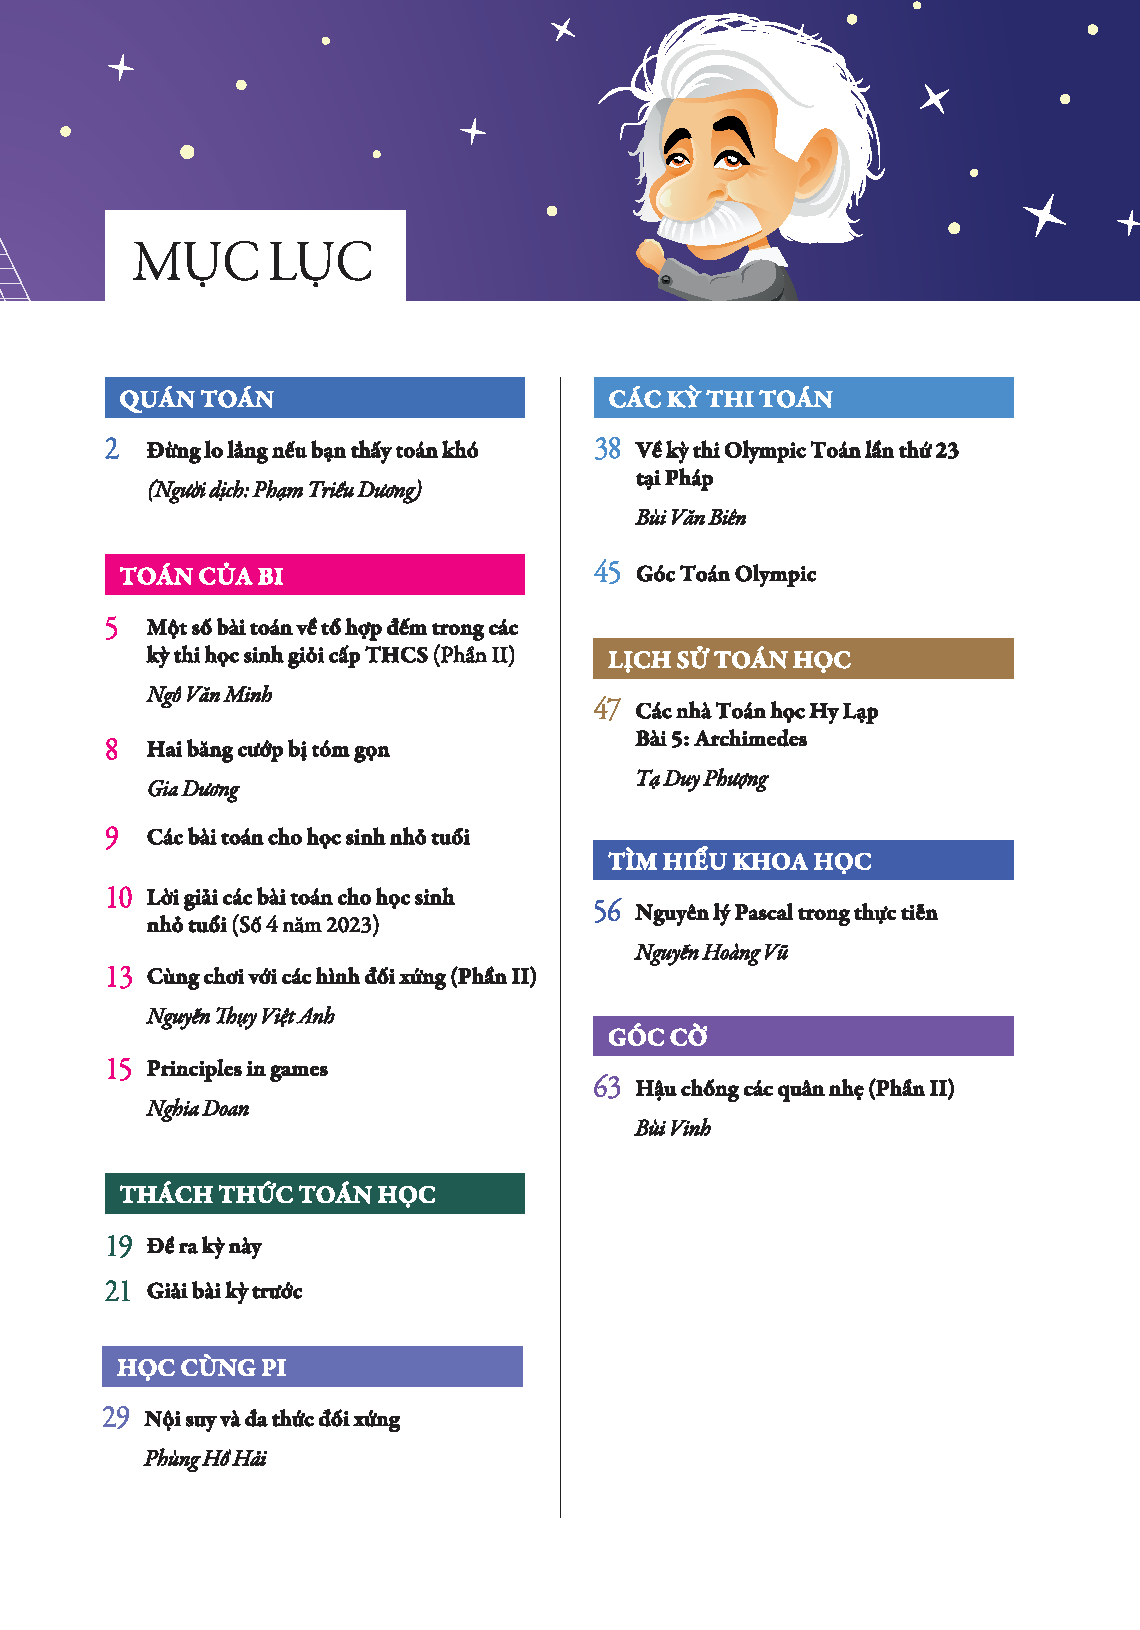
\includegraphics[scale=1]{ML.pdf}}}
%	 \centering
%	 \vspace*{0cm}
%	 \endgroup
%	 \newpage	  
%	 \pagestyle{empty}
%
	\setcounter{page}{2}
	\setcounter{figure}{0}
	\thispagestyle{toanhocvadoisongnone}
\pagestyle{toanhocvadoisong}
\everymath{\color{toanhocdoisong}}
\graphicspath{{../toanhocdoisong/pic/}}
\blfootnote{$^1$\color{toanhocdoisong}Hà Nội.}
\begingroup
\AddToShipoutPicture*{\put(0,616){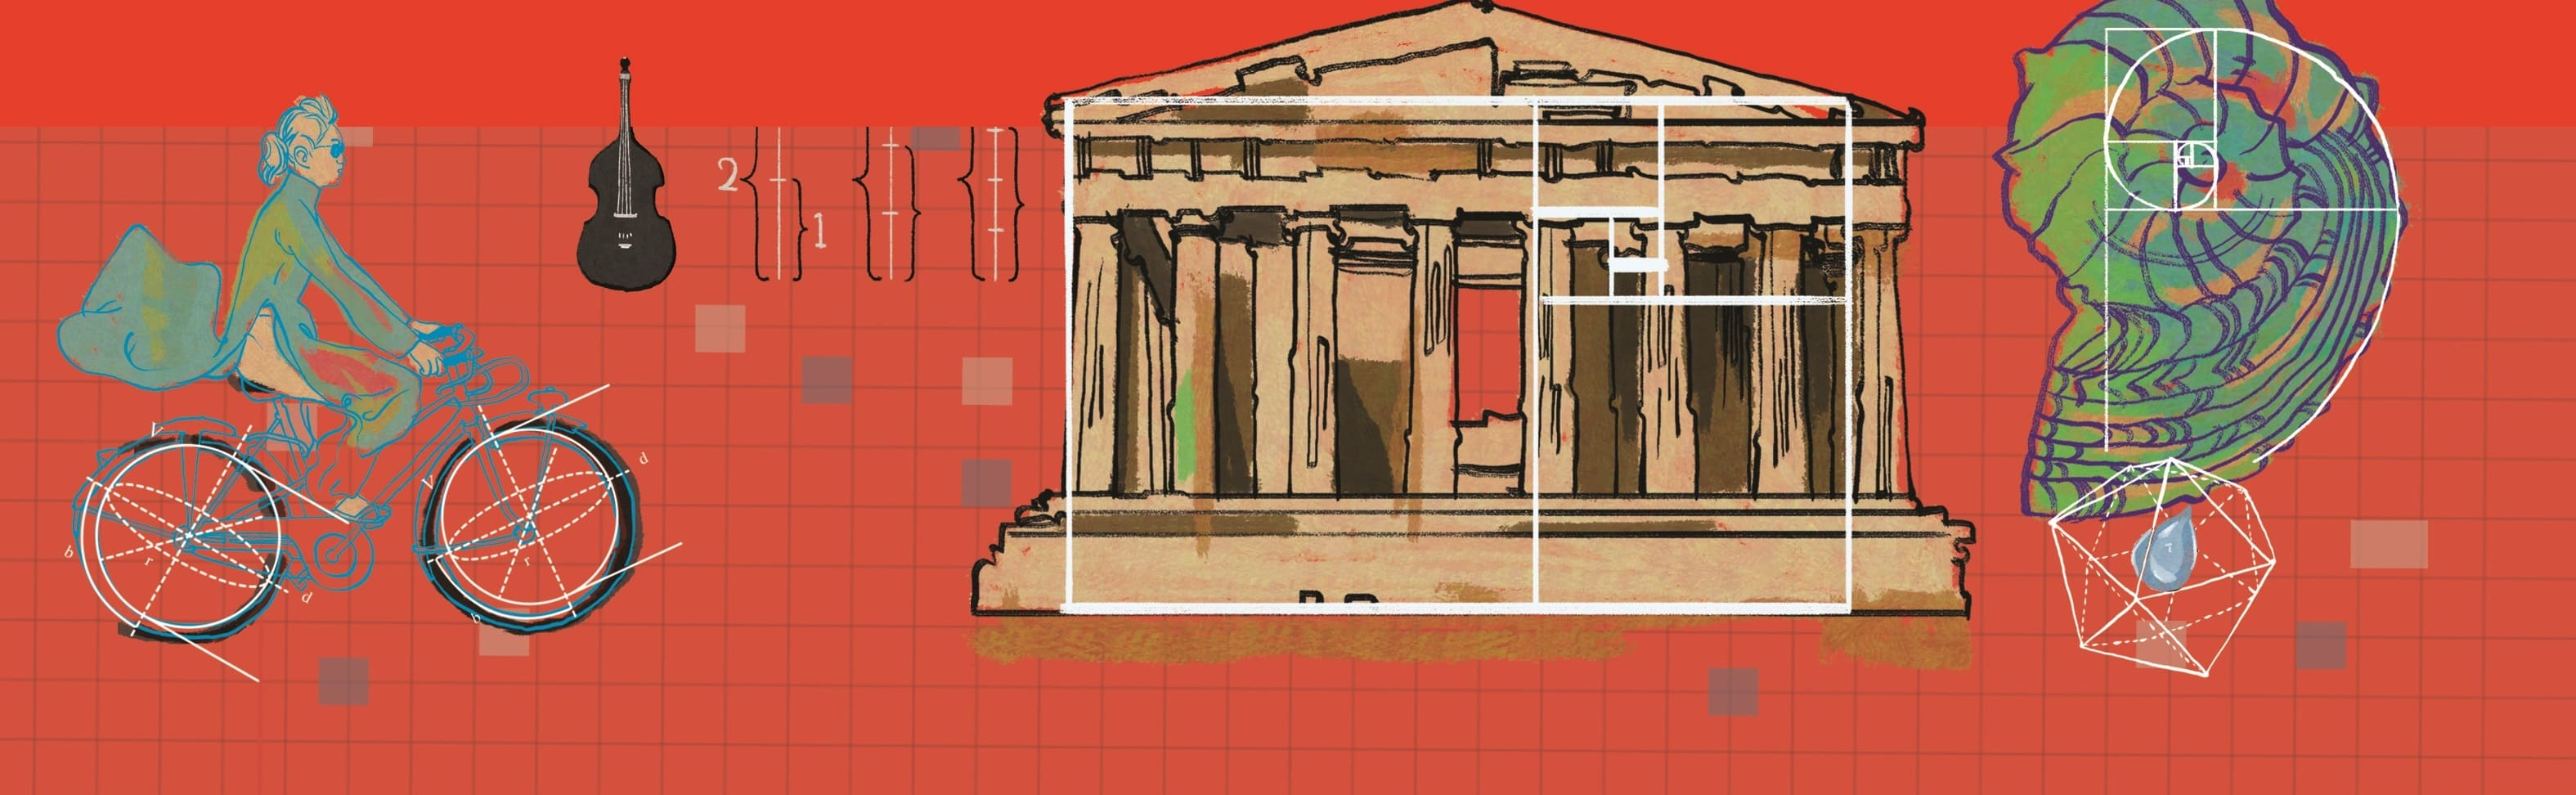
\includegraphics[width=19.3cm]{../bannertoanhocdoisong}}}
\AddToShipoutPicture*{\put(88,524){
\includegraphics[scale=1]{../tieude.pdf}}}
\centering
\endgroup

\vspace*{182pt}

\begin{multicols}{2}
	Việc quản lý lượng hàng lưu trong kho là một vấn đề quan trọng trong thương nghiệp. Đây cũng là một bài toán cơ bản của ngành vận trù học. Trong bài viết này, chúng ta hãy cùng tìm hiểu một số mô hình toán học để tìm chi phí tối thiểu cho các tình huống khác nhau khi lưu trữ hàng trong kho.
	\vskip 0.1cm
	$\pmb{1.}$ \textbf{\color{toanhocdoisong}Ford Harris và mô hình EOQ cổ điển}
	\begin{figure}[H]
		\vspace*{-5pt}
		\centering
		\captionsetup{labelformat= empty, justification=centering}
		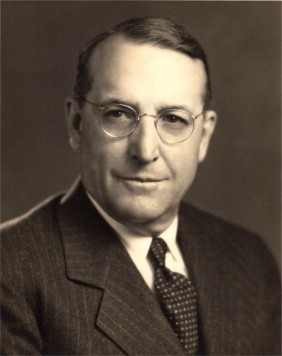
\includegraphics[width= 0.6\linewidth]{1}
		\caption{\small\textit{\color{toanhocdoisong}Ford Whitman Harris ($1877-1962$).}}
		\vspace*{-10pt}
	\end{figure}
	Mô hình EOQ (Economic Order Quantity) được Ford Whitman Harris, một kỹ sư lúc đó đang làm tư vấn về luật liên quan đến các bằng sáng chế, công bố năm $1913$. Đây là một mô hình đơn giản nhưng có tính thực tiễn cao về việc quản lý lượng hàng trong kho và vẫn có vai trò quan trọng trong ngành vận trù học ngày nay. 
	\vskip 0.1cm
	Mô hình EOQ này nhận các thông số đầu vào như sau:
	\vskip 0.1cm
	$K$: chi phí thiết lập cho một đơn hàng
	\vskip 0.1cm
	$c$: chi phí để sản xuất hoặc mua một đơn vị hàng
	\vskip 0.1cm
	$h$: chi phí để lưu một đơn vị hàng trong kho trong một đơn vị thời gian.
	\vskip 0.1cm
	Giả sử rằng nhu cầu tiêu thụ là đều theo thời gian và có giá trị $d$ đơn vị hàng/đơn vị thời gian. Nếu mỗi lần đặt hàng, ta đặt một lượng $Q$ đơn vị hàng thì số lượng hàng này sẽ được tiêu thụ hết trong thời gian $Q/d$. Chi phí cho một lần đặt hàng sẽ là $K+cQ$.
	\vskip 0.1cm
	Do lượng hàng sẽ giảm dần tuyến tính theo thời gian khi được bán ra, từ lúc nhận được $Q$ đơn vị hàng này đến khi tiêu thụ hết, số lượng đơn vị hàng trung bình được lưu trong kho từ đơn hàng này sẽ là $\dfrac{Q + 0}{2} = \dfrac{Q}{2}$. Chi phí lưu kho của đơn hàng cho đến khi bán hết sẽ là:
	\begin{align*}
		h\cdot \frac{Q}{2}\cdot \frac{Q}{d}=\frac{hQ^2}{2d}.
	\end{align*}
	Tổng chi phí cho một chu kỳ hàng sẽ là:
	\begin{align*}
		K + cQ + \frac{hQ^2}{2d}.
	\end{align*}
	Chi phí trong một đơn vị thời gian là:
	\begin{align*}
		T = \frac{K + cQ + \frac{hQ^2}{2d}}{\frac{Q}{d}} = \frac{dK}{Q} + dc + \frac{hQ}{2}.
	\end{align*}
	Ta cần tìm giá trị $Q^*$ sao cho $T$ nhận giá trị cực tiểu. Lấy đạo hàm của $T$ theo $Q$ được:
	\begin{align*}
		-\frac{dK}{Q^2} + \frac{h}{2} = 0.
	\end{align*}
	hay $Q^* = \sqrt{\dfrac{2dK}{h}}$.
	\vskip 0.1cm
	Nếu vẽ đồ thị của hàm $T(Q)$, ta được dạng đồ thị như trong Hình $1$. Hình dạng này của đồ thị hàm số có vai trò quan trọng trong một số bài toán ở các phần tiếp theo.
	\begin{figure}[H]
		\vspace*{-5pt}
		\centering
		\captionsetup{labelformat= empty, justification=centering}
		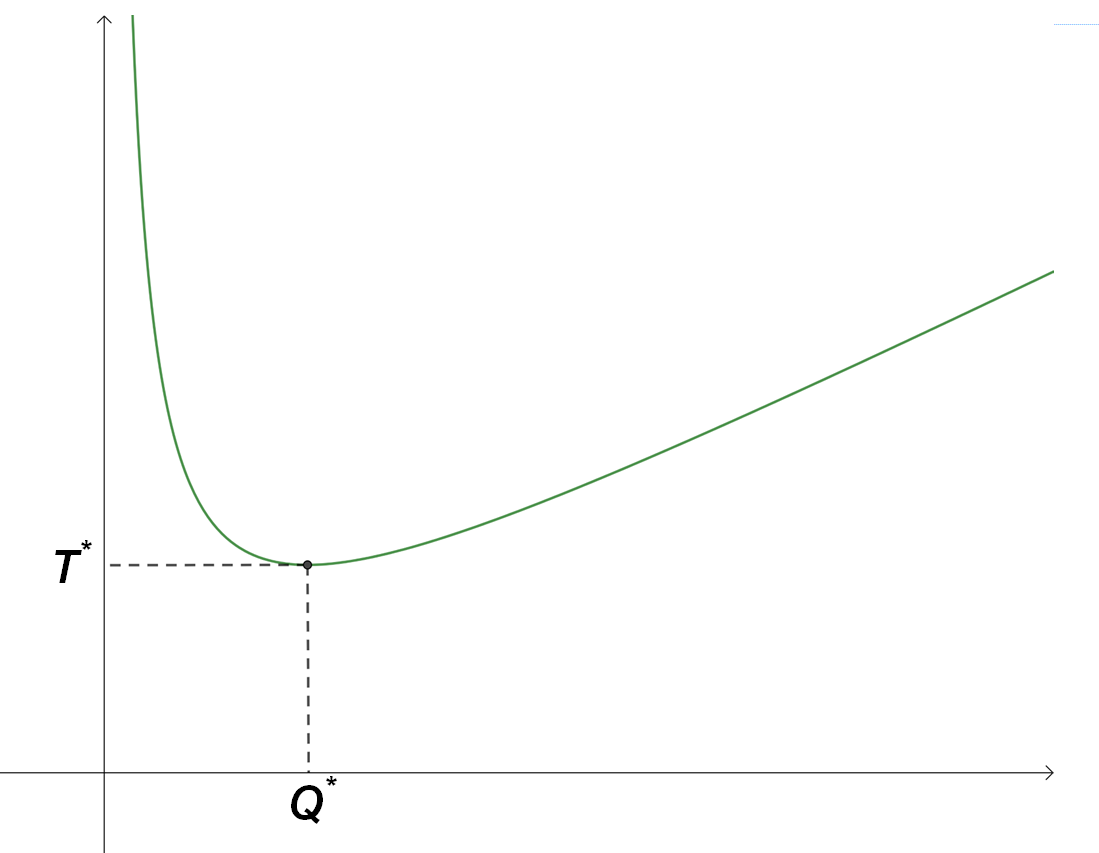
\includegraphics[width= 1\linewidth]{2}
		\caption{\small\textit{\color{toanhocdoisong}Hình $1$. Đồ thị của $T(Q)$.}}
		\vspace*{-10pt}
	\end{figure}
	Công thức EOQ dạng như trên xuất hiện ở nhiều giáo trình chuyên ngành kinh tế. Sau khi được Harris công bố năm $1913$, nó được nhiều tài liệu nhắc đến trong các thập kỷ sau đó (thường không có trích dẫn). Nhiều người gọi tên công thức này theo các tài liệu hoặc giáo trình mà họ biết. Vì lý do này, công thức EOQ còn được gọi là công thức Wilson hay công thức Camp. Trong khi đó, nguồn gốc từ Harris của công thức EOQ bị lãng quên cho đến khi được Donald Erlenkotter phát hiện lại vào năm $1988$. Một trong những nguyên nhân của vấn đề này có lẽ là do bản thân Harris không phải là một học giả. Tuy chỉ học hết cấp $3$, Harris đã tự phấn đấu và học việc để trở thành một kỹ sư với nhiều bằng sáng chế. Sau đó, ông tiếp tục tự học và có một sự nghiệp thành công trong lĩnh vực luật về các bằng sáng chế. Bản thân Harris cũng không cố gắng đạt được sự công nhận cho công thức EOQ cho đến khi mất vào năm $1962$. Ông luôn cho rằng các sáng chế mang tính thực tiễn có giá trị hơn những ý tưởng trừu tượng.
	\vskip 0.1cm
	$\pmb{2.}$ \textbf{\color{toanhocdoisong}Mô hình EOQ có cho phép thiếu hụt}
	\vskip 0.1cm
	Trong thiết lập trên, ta chưa xét thời gian từ lúc đặt hàng cho đến khi hàng về kho. Trong thực tế, việc này không phải là ngay lập tức và việc sản xuất hoặc vận chuyển cần tốn một khoảng thời gian $L$ nào đó. Do đó, khi lượng hàng trong kho chỉ còn $Ld$ (đủ dùng cho khoảng thời gian $L$) thì ta phải đặt lượng hàng $Q^*$.
	\begin{figure}[H]
		\vspace*{-5pt}
		\centering
		\captionsetup{labelformat= empty, justification=centering}
		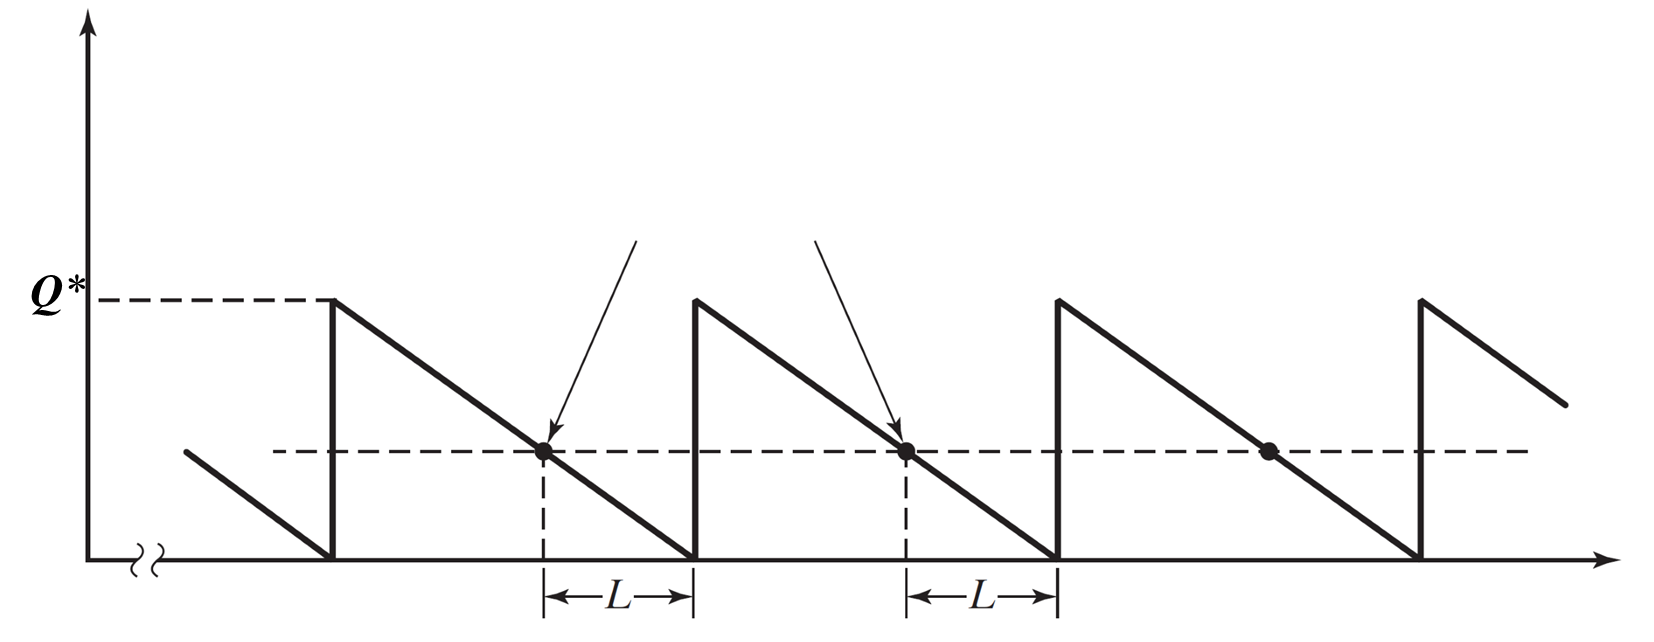
\includegraphics[width= 1\linewidth]{3}
		\caption{\small\textit{\color{toanhocdoisong}Hình $2$. Để tránh thiếu hụt, người ta cần đặt hàng khi lượng hàng còn lại trong kho đủ lớn sao cho trong khoảng thời gian này, thiếu hụt không xảy ra.}}
		\vspace*{-10pt}
	\end{figure}
	Mô hình này cũng có thể mở rộng trong trường hợp việc thiếu hụt là được cho phép. Nếu có nhu cầu cho hàng hóa mà hiện tại trong kho không có thì việc này được diễn tả bởi chi phí $p$, là chi phí phạt do thiếu hụt một đơn vị hàng trong một đơn vị thời gian. Trong thực tế, chi phí này có thể ứng với việc khách hàng mua hàng của công ty khác hoặc ta phải giảm giá cho khách hàng do họ phải đợi, ... Việc cân bằng giữa chi phí phạt do thiếu hụt và chi phí lưu hàng cho kho sẽ cho ta phương án với chi phí thấp nhất.
	\vskip 0.1cm
	Giả sử mỗi lần đặt hàng có lượng hàng là $Q$. Do có sự thiếu hụt nên sau khi giải quyết hết thiếu hụt, lượng hàng vào kho sẽ là $S$. Lượng hàng chịu chi phí do thiếu hụt sẽ là $Q-S$. Trong một chu kỳ thời gian $\dfrac{Q}{d}$, khoảng thời gian $\dfrac{S}{d}$ ban đầu sẽ không có thiếu hụt nhưng có chi phí lưu hàng trong kho còn khoảng thời gian còn lại không có hàng lưu kho.
	\begin{figure}[H]
		\vspace*{-5pt}
		\centering
		\captionsetup{labelformat= empty, justification=centering}
		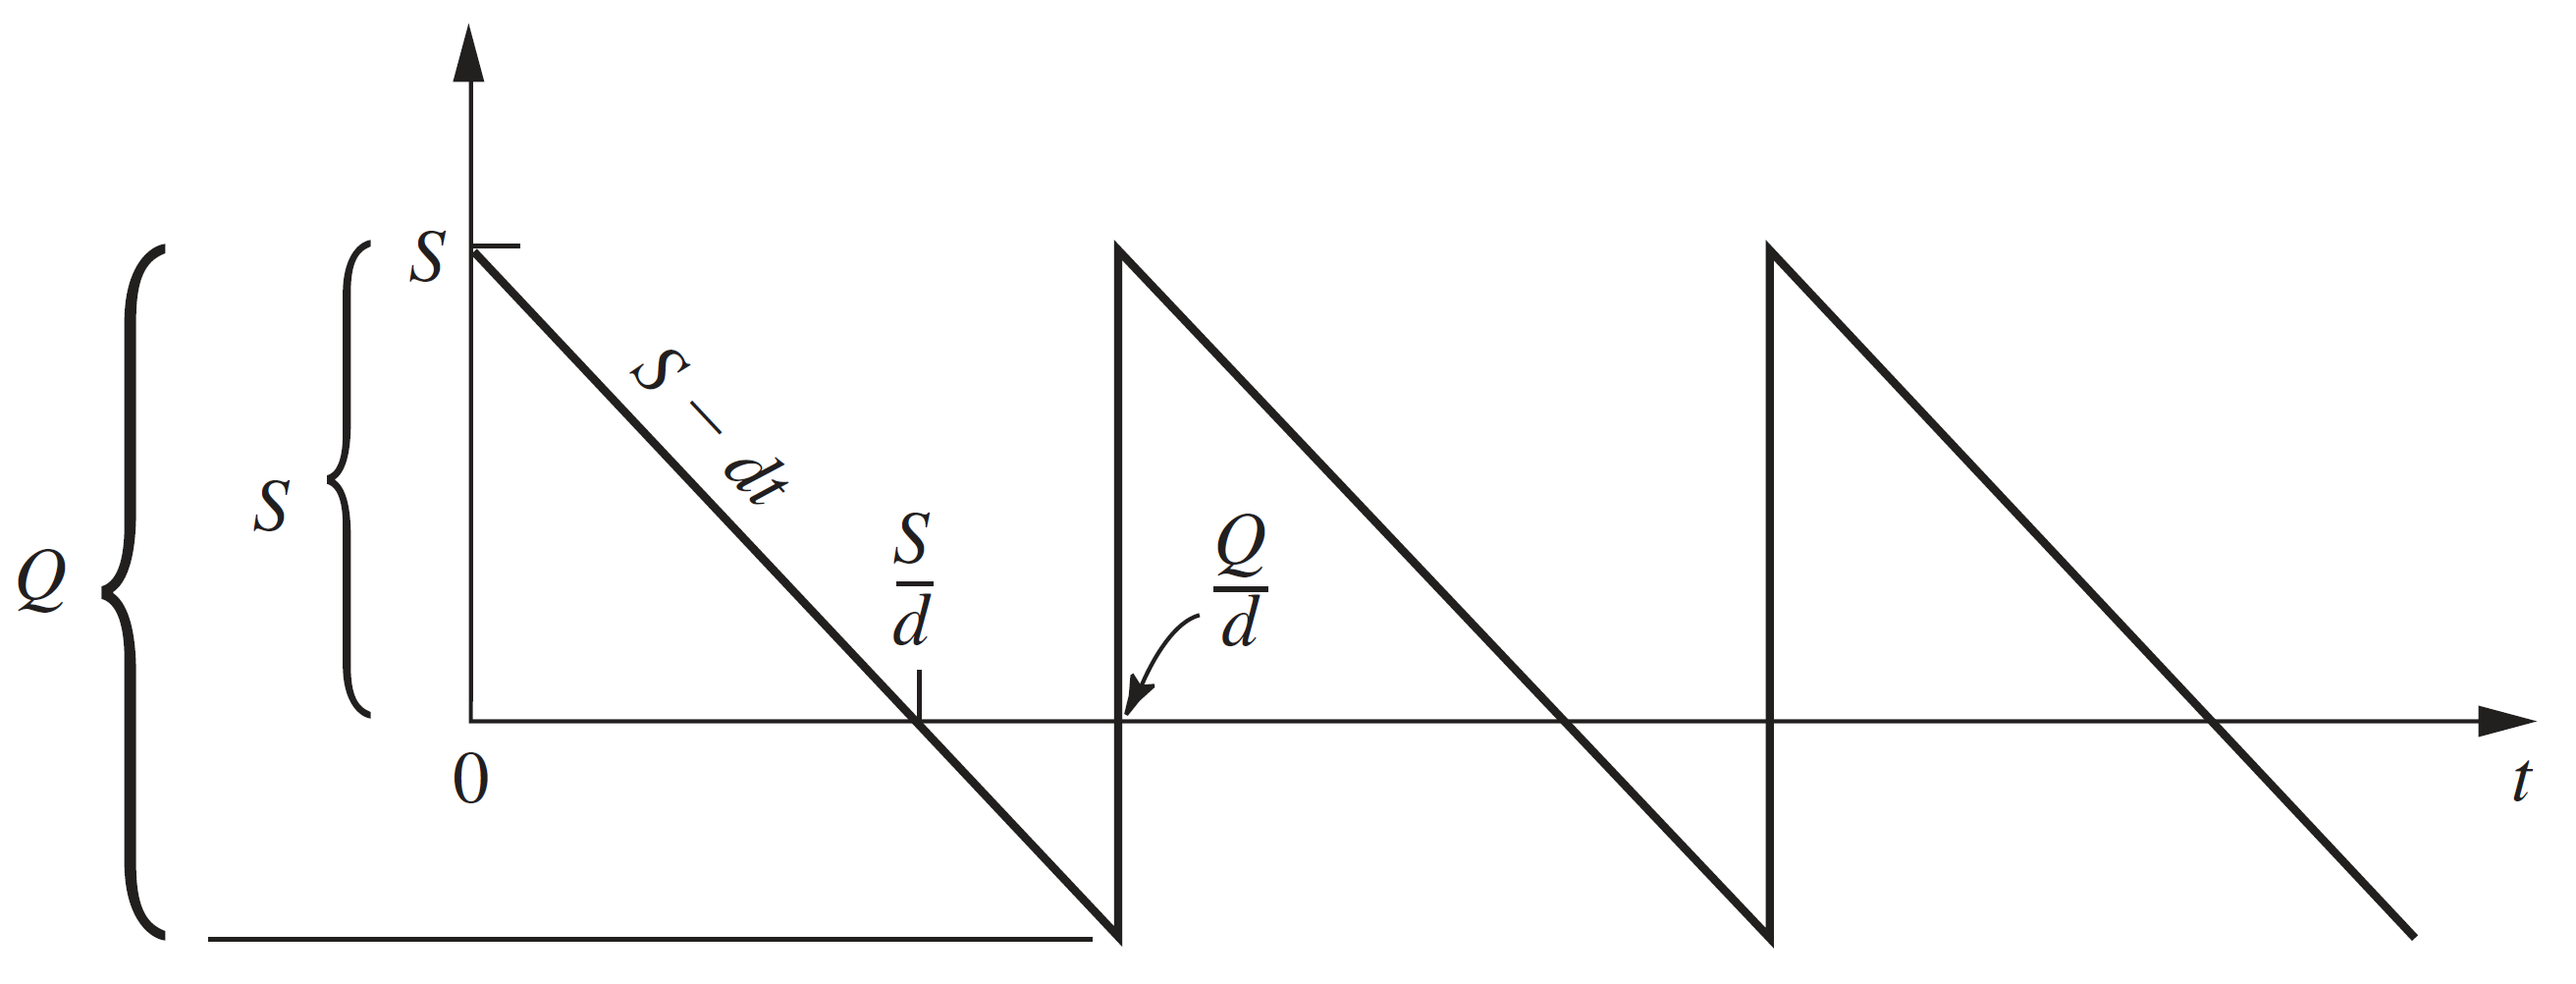
\includegraphics[width= 1\linewidth]{4}
		\caption{\small\textit{\color{toanhocdoisong}Hình $3$. Mô hình $EOQ$ có cho phép thiếu hụt xảy ra.}}
		\vspace*{-10pt}
	\end{figure}
	Tương tự với phần trên, chi phí đặt hàng vẫn là $K+cQ$ nhưng chi phí lưu kho trong một chu kỳ sẽ là
	\begin{align*}
		h\cdot\frac{S}{2}\cdot\frac{S}{d} = \frac{hS^2}{2d}.
	\end{align*}
	Trong khoảng thời gian thiếu hụt, lượng thiếu hụt trung bình sẽ là $\dfrac{Q-S}{2}$ nên chi phí phát sinh do thiếu hụt trong một chu kỳ sẽ là:
	\begin{align*}
		p\cdot\frac{Q-S}{2}\cdot\frac{Q-S}{d} = \frac{p(Q-S)^2}{2d}.
	\end{align*}
	Tổng chi phí trong một chu kỳ sẽ là:
	\begin{align*}
		K + cQ + \frac{hS^2}{2d} + \frac{p(Q-S)^2}{2d}.
	\end{align*}
	Tổng chi phí trong một đơn vị thời gian là:
	\begin{align*}
		T &= \frac{K + cQ + \frac{hS^2}{2d} + \frac{p(Q-S)^2}{2d}}{\frac{Q}{d}}\\
		 &= \frac{Kd}{Q} + cd + \frac{hS^2}{2Q} + \frac{p(Q-S)^2}{2Q}.
	\end{align*}
	Trong trường hợp này, cả $Q$ và $S$ đều thay đổi được nên $T$ là một hàm số của cả $Q$ lẫn $S$. Đây là một hàm số nhiều biến chứ không phải hàm số một biến như trong toán phổ thông. Vậy phải làm sao để tìm giá trị của $Q$ và $S$ để $T$ cực tiểu?
	\vskip 0.1cm
	Cần nhớ lại rằng, với hàm số một biến dạng $y=f(x)$ thì đạo hàm $\dfrac{dy}{dx}$ cho ta biết tốc độ biến thiên của $y$ khi $x$ thay đổi. Với những hàm số nhiều biến, để biểu diễn tốc độ biến thiên của nó khi một trong các biến thay đổi, người ta sử dụng khái niệm đạo hàm riêng. Đạo hàm riêng được tính cho từng biến. Trong trường hợp $T$, nó là hàm số $T(Q,S)$ của cả hai biến $Q$ và $S$ nên ta có hai đạo hàm riêng, một cho $Q$ (ký hiệu $\dfrac{\partial T}{\partial Q}$) và một cho $S$ (ký hiệu $\dfrac{\partial T}{\partial S}$) . Việc tính đạo hàm riêng cũng không khác là mấy so với tính đạo hàm của hàm số một biến. Khi lấy đạo hàm riêng theo một biến, ta coi các biến còn lại không đổi và áp dụng các quy tắc giống như khi lấy đạo hàm của hàm số một biến.
	\vskip 0.1cm
	Trong trường hợp hàm $T(Q,S)$, ta có:
	\begin{align*}
		&\frac{\partial T}{\partial S} = \frac{hS}{Q} - \frac{p(Q-S)}{Q},\\
		&\frac{\partial T}{\partial Q} = \!- \frac{dK}{Q^2} \!-\! \frac{hS^2}{2Q^2} \!+\! \frac{p(Q\!-\!S)}{Q} \!-\! \frac{p(Q\!-\!S)^2}{2Q^2}.
	\end{align*}
	Để tìm cực trị của hàm nhiều biến, ta tìm điểm mà tại đó các đạo hàm riêng của nó bằng $0$ (tương tự như việc dùng đạo hàm để tìm cực trị của hàm số một biến). Với $T$, điều kiện này tương đương với hệ phương trình:
	\begin{align*}
		\begin{cases}
			\frac{hS}{Q} - \frac{p(Q-S)}{Q}= 0\\
			\!-\!\frac{dK}{Q^2} \!-\! \frac{hS^2}{2Q^2} \!+\! \frac{p(Q\!-\!S)}{Q} \!-\! \frac{p(Q\!-\!S)^2}{2Q^2}\!=\! 0.
		\end{cases}
	\end{align*}
	Hệ phương trình này tương đương với:
	\begin{align*}
		\begin{cases}
			S = \frac{p}{p+h}Q\\
			\!-\!dK \!-\! \frac{hS^2}{2} \!+\! p(Q-S)Q \!-\! \frac{p}{2}(Q\!-\!S)^2 \!=\! 0
		\end{cases}
	\end{align*}
	Tiến hành thế sử dụng biểu thức của $S$ theo $Q$ ta có:
	\begin{align*}
		&-dK \!-\! \frac{h}{2}\left(\!\!\frac{p}{p+h}\!\!\right)^2Q^2 \!+\! p\left(\!\!Q \!-\! \frac{p}{p+h}Q\!\right)\!Q \\
		&- \frac{p}{2}\left(Q - \frac{p}{p+h}Q\right)^2 = 0\\
		&-dK - \frac{h}{2}\left(\frac{p}{p+h}\right)^2Q^2 + \frac{ph}{p+h}Q^2 \\
		&- \frac{ph^2}{2(p+h)^2}Q^2 = 0\\
		&\frac{1}{2}\frac{\left(-p^2h + 2ph(p+h)-ph^2\right)}{(p+h)^2}Q^2 = dK\\
		&\frac{1}{2}\cdot\frac{ph(p+h)}{(p+h)^2}Q^2 = dK\\
		&Q^2 = \frac{2dK}{h}\cdot\frac{p+h}{p}.
	\end{align*}
	Ta được các giá trị của $S$ và $Q$ tại điểm cực trị:
	\begin{align*}
		Q^*\!=\!\sqrt{\frac{2dK}{h}}\sqrt{\!\frac{p+h}{p}},S^*\!=\! \sqrt{\!\frac{2dK}{h}}\sqrt{\!\frac{p}{p+h}}.
	\end{align*}
	Khi đó, chu kỳ tối ưu của việc đặt hàng sẽ là:
	\begin{align*}
		t^* = \frac{Q^*}{d}= \sqrt{\dfrac{2K}{dh}}\sqrt{\dfrac{p+h}{p}}.
	\end{align*}
	Số đơn vị hàng có tình trạng thiếu sẽ là:
	\begin{align*}
		Q^*- S^* = \sqrt{\dfrac{2dK}{p}}\sqrt{\dfrac{h}{p+h}}.
	\end{align*}
	Chính sách nhập hàng của ta sẽ thay đổi theo các giá trị của $h$ và $p$. Khi $p \to \infty$ còn $h$ không đổi, $Q^*-S^* \to 0$ và ta trở lại mô hình EOQ cơ bản: chi phí thiệt hại khi có thiếu hụt là quá lớn nên việc thiếu hụt không được phép xảy ra. Ngược lại, nếu $h \to \infty$ với $p$ không đổi (chi phí giữ hàng trong kho rất lớn so với thiệt hại do thiếu hụt), thì $S^* \to 0$ hay việc sử dụng kho hàng là không khả thi về mặt kinh tế và tất cả các nhu cầu mua hàng đều không được đáp ứng ngay mà được gom lại và giải quyết theo từng đợt mà không có lưu kho.
	\vskip 0.1cm
	$\pmb{3}$ \textbf{\color{toanhocdoisong}Mô hình EOQ với giá thành phân tầng}
	\vskip 0.1cm
	Ta hãy xử lý một tình huống khá thú vị xuất phát từ thực tế. Khi đặt hàng, nếu số lượng hàng vượt quá một ngưỡng $q$ nào đó, giá mua vào có thể được chiết khấu giảm đi. Ta hãy xét hàm chi phí mua vào cho một đơn vị hàng như sau:
	\begin{align*}
		c(Q)= \begin{cases}
			c_1,Q <q\\
			c_2,Q \ge q
		\end{cases}
	\end{align*}
	với $c_2<c_1$.
	\vskip 0.1cm
	Ta được hai hàm chi phí ứng với hai giá mua này (để đơn giản, trường hợp có thiếu hụt không được cho phép):
	\begin{align*}
		T_1 = \dfrac{dK}{Q} + c_1d  + \frac{hQ}{2},\\
		T_2 = \frac{dK}{Q} + c_2d + \frac{hQ}{2}.
	\end{align*}
	$T_2$ có hình dạng đồ thị giống hệt $T_1$ nhưng được tịnh tiến xuống một khoảng $(c_1-c_2 )d$ theo trục $y$. Hai đồ thị này đều có giá trị cực tiểu tại $Q=Q^*$. Ta cần chú ý đến điểm $Q_1>Q^*$ có $T_1 (Q_1 )=T_2 (Q^*)$ và dùng điểm này để biện luận các trường hợp (bạn đọc có thể tự giải để tìm $Q_1$, nó sẽ là nghiệm của một phương trình bậc hai).
	\begin{figure}[H]
		\vspace*{-5pt}
		\centering
		\captionsetup{labelformat= empty, justification=centering}
		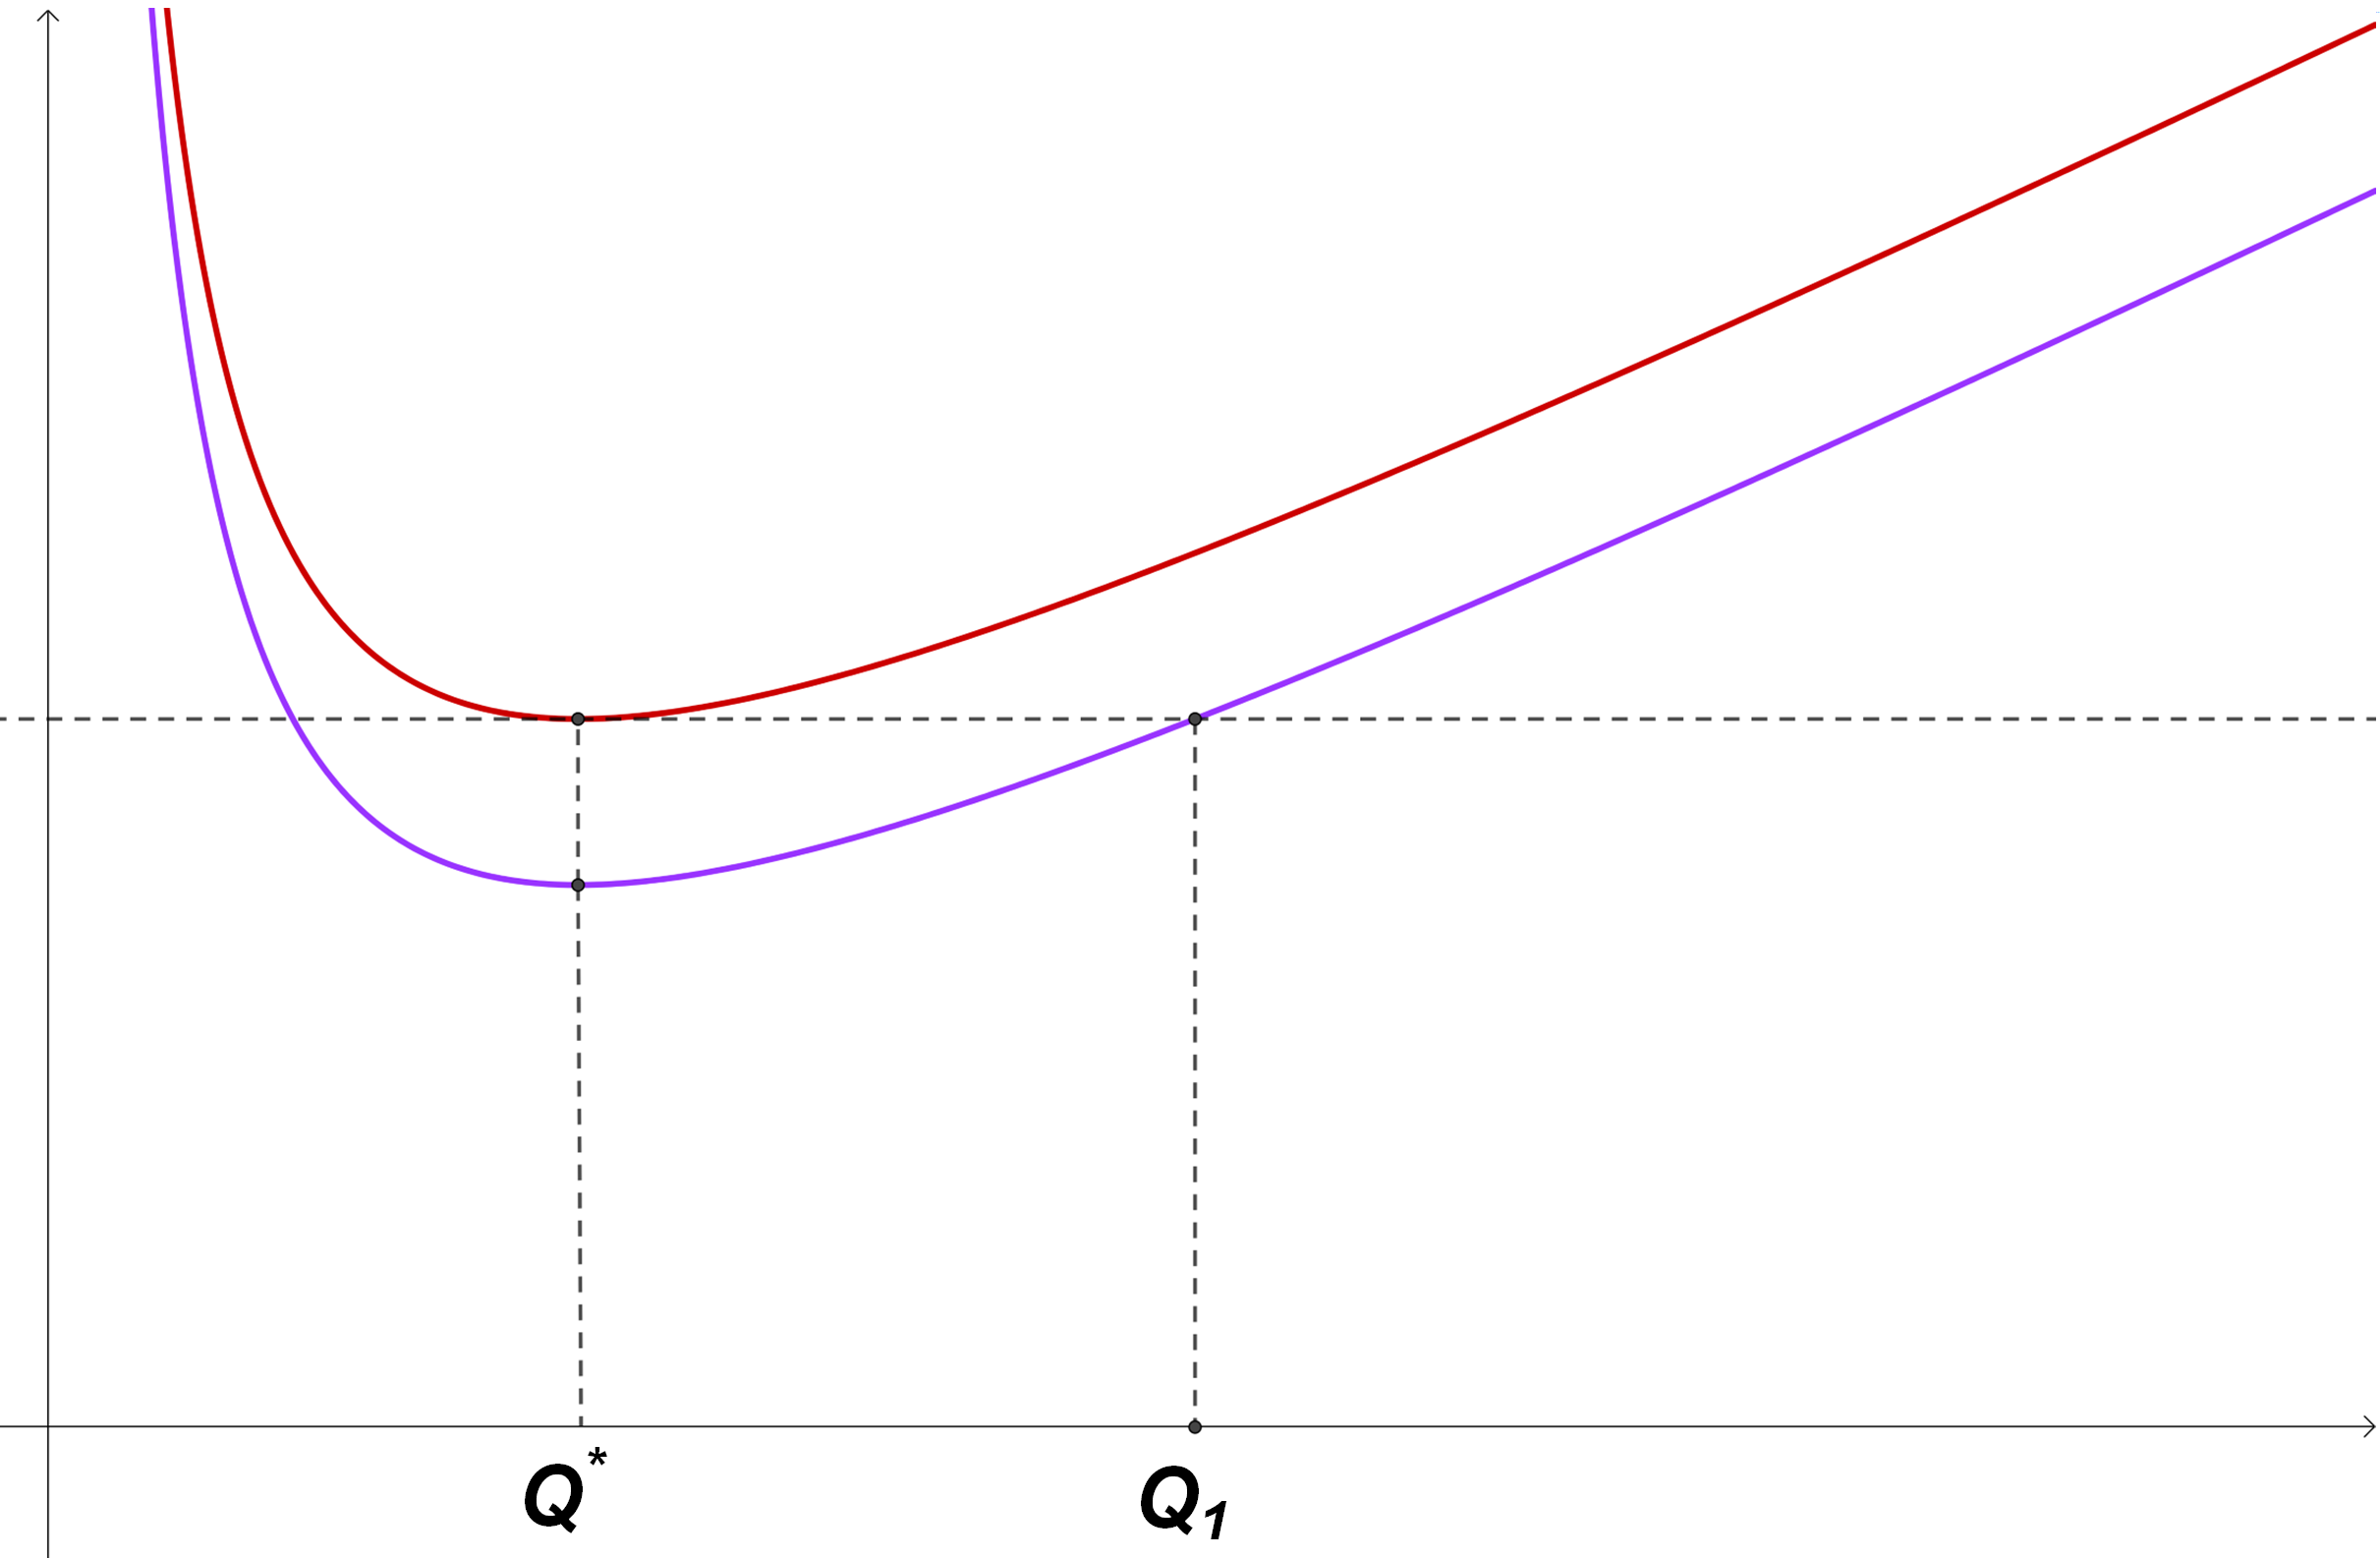
\includegraphics[width= 1\linewidth]{5}
		\caption{\small\textit{\color{toanhocdoisong}Hình $4$. Đồ thị của $T_1(Q)$ và $T_2(Q)$.}}
		\vspace*{-10pt}
	\end{figure}
	Hàm chi phí của ta sẽ có dạng:
	\begin{align*}
		T(Q) = \begin{cases}
			T_1(Q),Q \le q\\
			T_2(Q),Q > q
		\end{cases}
	\end{align*}
	Những hàm số như trên còn được gọi là hàm số liên tục theo từng đoạn. Để tìm cực tiểu của nó, ta cần xét $3$ trường hợp khác nhau.
	\vskip 0.1cm
	$\bullet$ Trường hợp $1$: $q<Q^*$.  Khi đó cực tiểu sẽ trùng với $Q=Q^*$ (Hình $5$).
	\begin{figure}[H]
		\vspace*{-5pt}
		\centering
		\captionsetup{labelformat= empty, justification=centering}
		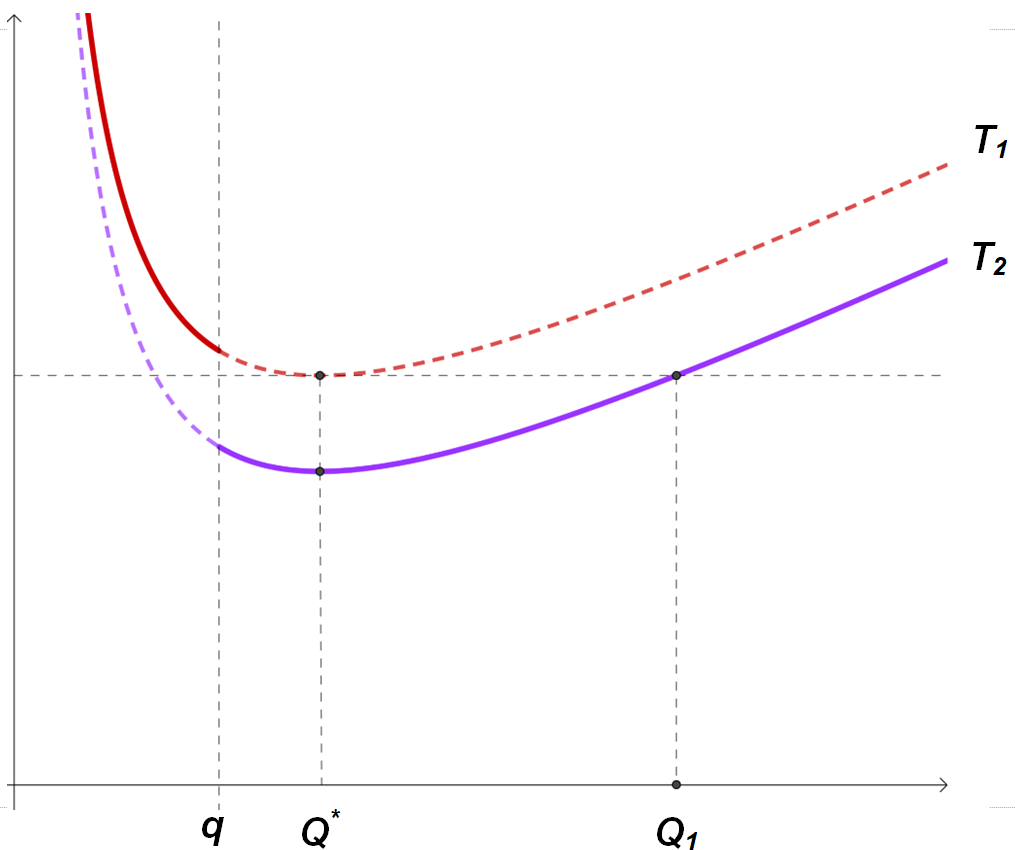
\includegraphics[width= 1\linewidth]{6}
		\caption{\small\textit{\color{toanhocdoisong}Hình $5$. Trường hợp $1$, $q<Q^*$.}}
		\vspace*{-10pt}
	\end{figure}
	$\bullet$ Trường hợp $2$: $Q^* \le q \le Q_1$. Nhìn vào Hình $6$, ta thấy cực tiểu sẽ đạt được khi $Q=q$. Ta mua hàng với số lượng nhỏ nhất để vẫn được mua với giá thấp hơn.
	\begin{figure}[H]
		\vspace*{-5pt}
		\centering
		\captionsetup{labelformat= empty, justification=centering}
		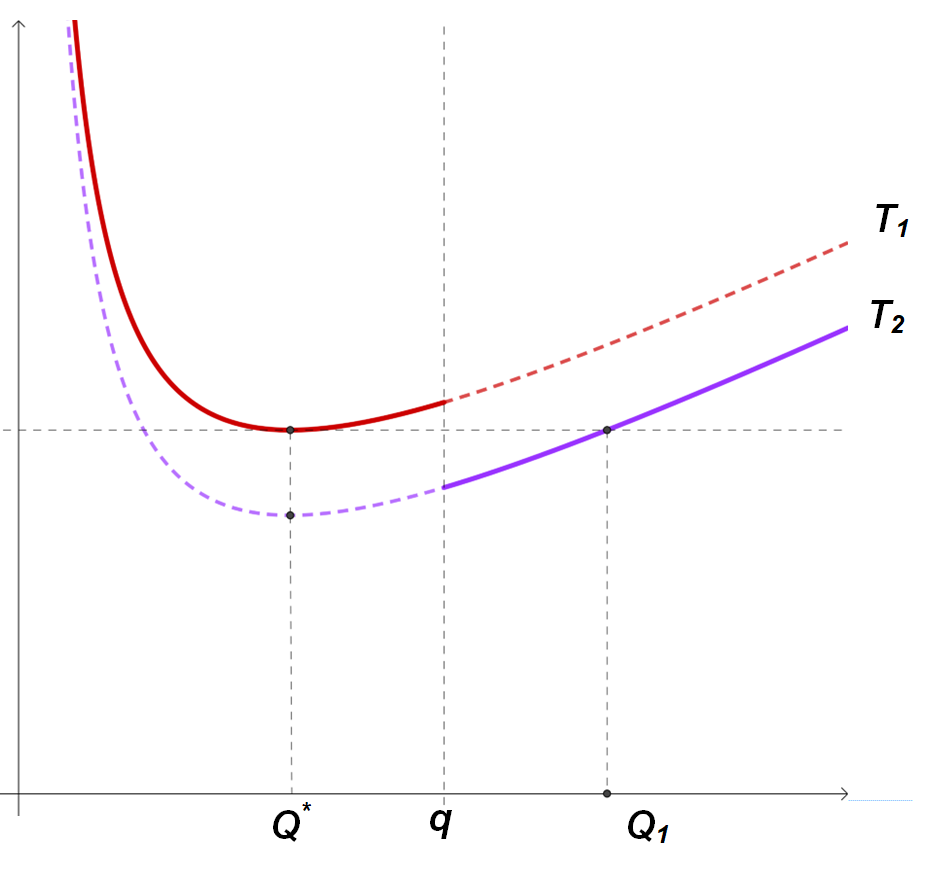
\includegraphics[width= 1\linewidth]{7}
		\caption{\small\textit{\color{toanhocdoisong}Hình $6$. Trường hợp $2$: $Q^* \le q \le Q_1$.}}
		\vspace*{-10pt}
	\end{figure}
	$\bullet$ Trường hợp $3$: $q>Q_1$. Tương tự trường hợp $1$, ta mua với số lượng $Q=Q^*$. Tuy không được hưởng chiết khấu nhưng chi phí lưu kho của ta vẫn nhỏ hơn so với việc mua nhiều để được chiết khấu.
	\begin{figure}[H]
%		\vspace*{-5pt}
		\centering
		\captionsetup{labelformat= empty, justification=centering}
		
\includegraphics[width= 1\linewidth]{8}
		\caption{\small\textit{\color{toanhocdoisong}Hình $7$. Trường hợp $3$: $q>Q_1$}}
		\vspace*{-10pt}
	\end{figure}
	Bạn đọc có thể thử tự giải cho trường hợp có nhiều hơn $2$ tầng phân khúc của giá hàng. Khi đó ta sẽ có một bài toán khảo sát hàm số liên tục từng đoạn tương đối thú vị.
	\vskip 0.1cm
	$\pmb{4.}$ \textbf{\color{toanhocdoisong}Mô hình EOQ ngẫu nhiên và bài toán sạp báo}
	\begin{figure}[H]
		\vspace*{-5pt}
		\centering
		\captionsetup{labelformat= empty, justification=centering}
		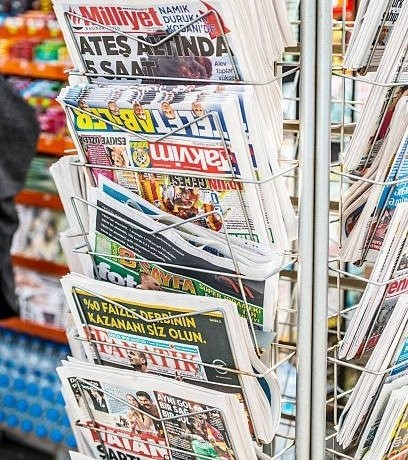
\includegraphics[width= 1\linewidth]{9}
		\caption{\small\textit{\color{toanhocdoisong}Hình $8$. Báo ra hàng ngày có giá trị giảm nhiều vào ngày hôm sau nên việc đặt mua bao nhiêu báo cũng là một vấn đề quan trọng của các sạp báo.}}
		\vspace*{-10pt}
	\end{figure}
	Ta hãy sử dụng mô hình EOQ để nghiên cứu một bài toán phức tạp hơn. Xét một sạp báo với lượng báo $S$ được đặt vào đầu buổi sáng. Nếu báo đặt không đủ nhu cầu, ta có chi phí phạt $p$ cho một đơn vị báo bị thiếu hụt, còn nếu báo đặt bị thừa, do nó là mặt hàng có giá trị suy giảm theo thời gian ta sẽ có chi phí $h$ để lưu trữ mỗi đơn vị sang ngày hôm sau (bao gồm chi phí giữ trong kho qua đêm trừ đi giá bán rẻ hơn vào ngày hôm sau).
	\vskip 0.1cm
	Gọi $D$ là nhu cầu trong ngày và giá một đơn vị báo mua vào là $c$. Chi phí của một ngày sẽ là:
	\begin{align*}
		C(D,S) = \,&cS + p\max(0,D - S) \\
		&+ h\max(0,S-D).
	\end{align*}
	Ở đây, chi phí phạt chỉ xuất hiện khi nhu cầu nhiều hơn lượng báo ta có, còn chi phí lưu trữ chỉ xuất hiện khi lượng báo nhiều hơn nhu cầu.
	\vskip 0.1cm
	Ta lại giả sử nhu cầu $D$ là một biến ngẫu nhiên với hàm mật độ xác suất $f(x)$. Khi đó, giá trị trung bình của chi phí của ta sẽ là:
	\begin{align*}
		C(S) =\,& E\left[C(D,S)\right] \\
			=\,& cS + \int_S^\infty  {p(x - S)f(x)dx} \\
			&+ \int_0^\infty  {h(S - x)f(x)dx.} 
	\end{align*}
	Chú ý rằng cận của hai tích phân trong biểu thức này ứng với phân tích ở trên về sự xuất hiện của $p$ và $h$ theo $S$ trong mô hình: $p$ chỉ có ý nghĩa khi $D>S$ và $h$ chỉ xuất hiện khi $D<S$.
	\vskip 0.2cm
	\PIbox{Với biến ngẫu nhiên nhận các giá trị liên tục, người ta sử dụng khái niệm hàm mật độ. Xác suất để biến ngẫu nhiên $X$ với hàm mật độ $f(x)$ nằm trong khoảng $[a,b]$ sẽ là $\int_a^b{f(x)dx}$.
	}
	\vskip 0.2cm
	Đến đây ta gặp phải vấn đề làm thế nào để tìm cực trị của một hàm số có chứa tích phân! Tuy rằng các công thức giải tích đại học có thể cho ta kết quả ngay, việc sử dụng các kiến thức toán phổ thông để tìm cực trị của $C(S)$ cũng không quá khó. Ta viết lại $C(S)$ dưới dạng:
	\begin{align*}
		&C(S) \\
		= \,&cS + p\int_S^{\infty}{xf(x)dx} - pS\int_S^{\infty}{f(x)dx}\\
		 &+ hS\int_0^{S}{f(x)dx} - h\int_0^{S}{xf(x)dx}\\
		= \,&cS \!+\! p\left[G(\infty) \!-\! G(S)\right] \!-\! pS\left[F(\infty) \!-\! F(S)\right]\\
		&+ hS\left[F(S) - F(0)\right] - h\left[G(S) - G(0)\right],
	\end{align*}
	với $F$ và $G$ lần lượt là nguyên hàm của $f(x)$ và $xf(x)$.
	\vskip 0.1cm
	Ta lấy đạo hàm của $C(S)$ theo $S$, (sử dụng các công thức $\dfrac{dF(S)}{dS} = f(S)$ và $\dfrac{dG(S)}{dS} = Sf(S)$):
	\begin{align*}
		&\frac{dC(S)}{dS} \\
		= \,&c - pSf(S) - pF(\infty) + pF(S) + pSf(S) \\
		&+ hF(S) + hSf(S) - hF(0) - hSf(S)\\
		= \,&c- p\left[F(\infty) - F(S)\right] + h\left[F(S) - f(0)\right]\\
		= \,&c- p\int_S^{\infty}{f(x)dx} + h\int_0^{S}{f(x)dx}.
	\end{align*}
	Chú ý rằng ở đây ta đã sử dụng dạng ngược của công thức Newton--Leibniz: $F(b)-F(a)= \int_a^b{f(x)dx}$. Trong trường hợp các hàm số $f(x)$ và $xf(x)$ không có nguyên hàm, ta cần tính đạo hàm theo giới hạn để tính đạo hàm của tích phân có cận phụ thuộc tham biến (xem phụ lục).
	\vskip 0.1cm
	Vì $f(x)$ là hàm mật độ xác suất nên $\int_0^{\infty}{f(x)dx} = 1$ (ứng với $P(0 \le D \le \infty)=1$). Do đó:
	\begin{align*}
		\int_0^{S}{f(x)dx} + \int_S^{\infty}{f(x)dx} = \int_0^{\infty}{f(x)dx}=1.
	\end{align*}
	Thay vào biểu thức của $\dfrac{dC(S)}{dS}$ ta được:
	\begin{align*}
		&\frac{dC(S)}{dS} \\
		= \,&c- p\left(1- \int_0^{S}{f(x)dx}\right) + h\int_0^{S}{f(x)dx} \\
		= \,&(c-p) + (p+h)\int_0^{S}{f(x)dx}.
	\end{align*}
	Để tìm cực trị, ta cho biểu thức trên bằng $0$ và được:
	\begin{align*}
		(p+h)\int_0^{S}{f(x)dx} = p-c,
	\end{align*}
	hay:
	\begin{align*}
		\int_0^{S}{f(x)dx} = \frac{p-c}{p+h}
	\end{align*}
	Do đó cực trị xuất hiện ở giá trị $S^*$ sao cho:
	\begin{align*}
		F(S^*) = \frac{p-c}{p+h}.
	\end{align*}
	Ở đây ta đã chọn $F(S)$ sao cho $F(0)=0$. Khi đó $F(x)$ trở thành hàm phân phối cộng dồn cho biến ngẫu nhiên $D$. Giá trị $F(x)$ sẽ bằng với xác suất $P(D \le x)$.
	\vskip 0.1cm
	Có thể thấy, việc sử dụng nguyên hàm và các công thức có liên quan cho phép ta tìm cực trị của một hàm số có chứa tích phân chỉ sau một vài biến đổi.
	\vskip 0.1cm
	Mô hình trên cho bài toán sạp báo cũng có thể được áp dụng cho các trường hợp khác trong thực tế khi người ta cần phải tính đến việc một số loại hàng hóa không giữ nguyên giá trị nếu bị lưu kho đến giai đoạn thời gian tiếp theo. Các ví dụ thường thấy bao gồm: thực phẩm, hoa, quần áo (ví dụ quần áo mùa đông khi mùa hè sắp đến), ...
	\vskip 0.1cm
	Trong trường hợp trước khi đặt hàng, cửa hàng vẫn còn tồn một lượng hàng hóa I từ trước đó thì chi phí của ta sẽ là:
	\begin{align*}
		\overline{C}(S) = C(S) - CI.
	\end{align*}
	Nếu $I<S^*$ thì ta chỉ cần đặt một lượng hàng hóa đúng bằng $S^*-I$.
	\vskip 0.1cm
	Trong trường hợp $I\ge S^*$, ta cần xét xem $C(S)$ đồng biến hay nghịch biến trong khoảng này. Do $f(x)>0$ với mọi $x$ nên $\dfrac{dC(S)}{dS}$ tăng khi $S$ tăng. Tại $S=S^*, \dfrac{dC(S)}{dS}=0$ nên $\dfrac{dC(S)}{dS}$ sẽ $>0$ với $S>S^*$. Vì vậy, trong trường hợp này, ta không đặt thêm hàng nữa mà chỉ bán hết lượng hàng $I$ còn trong kho.
	\vskip 0.1cm
	Nếu có thêm chi phí thiết lập đơn hàng $K$ thì hàm chi phí của ta có giá trị như sau:
	\vskip 0.1cm
	$\overline{C}(S) = K + C(S) - cI$ nếu đơn hàng được đặt
	và $\overline{C}(S) = C(I)- cI$ nếu không đặt hàng mà chi bán nốt hàng trong kho.
	\begin{figure}[H]
		\vspace*{-5pt}
		\centering
		\captionsetup{labelformat= empty, justification=centering}
		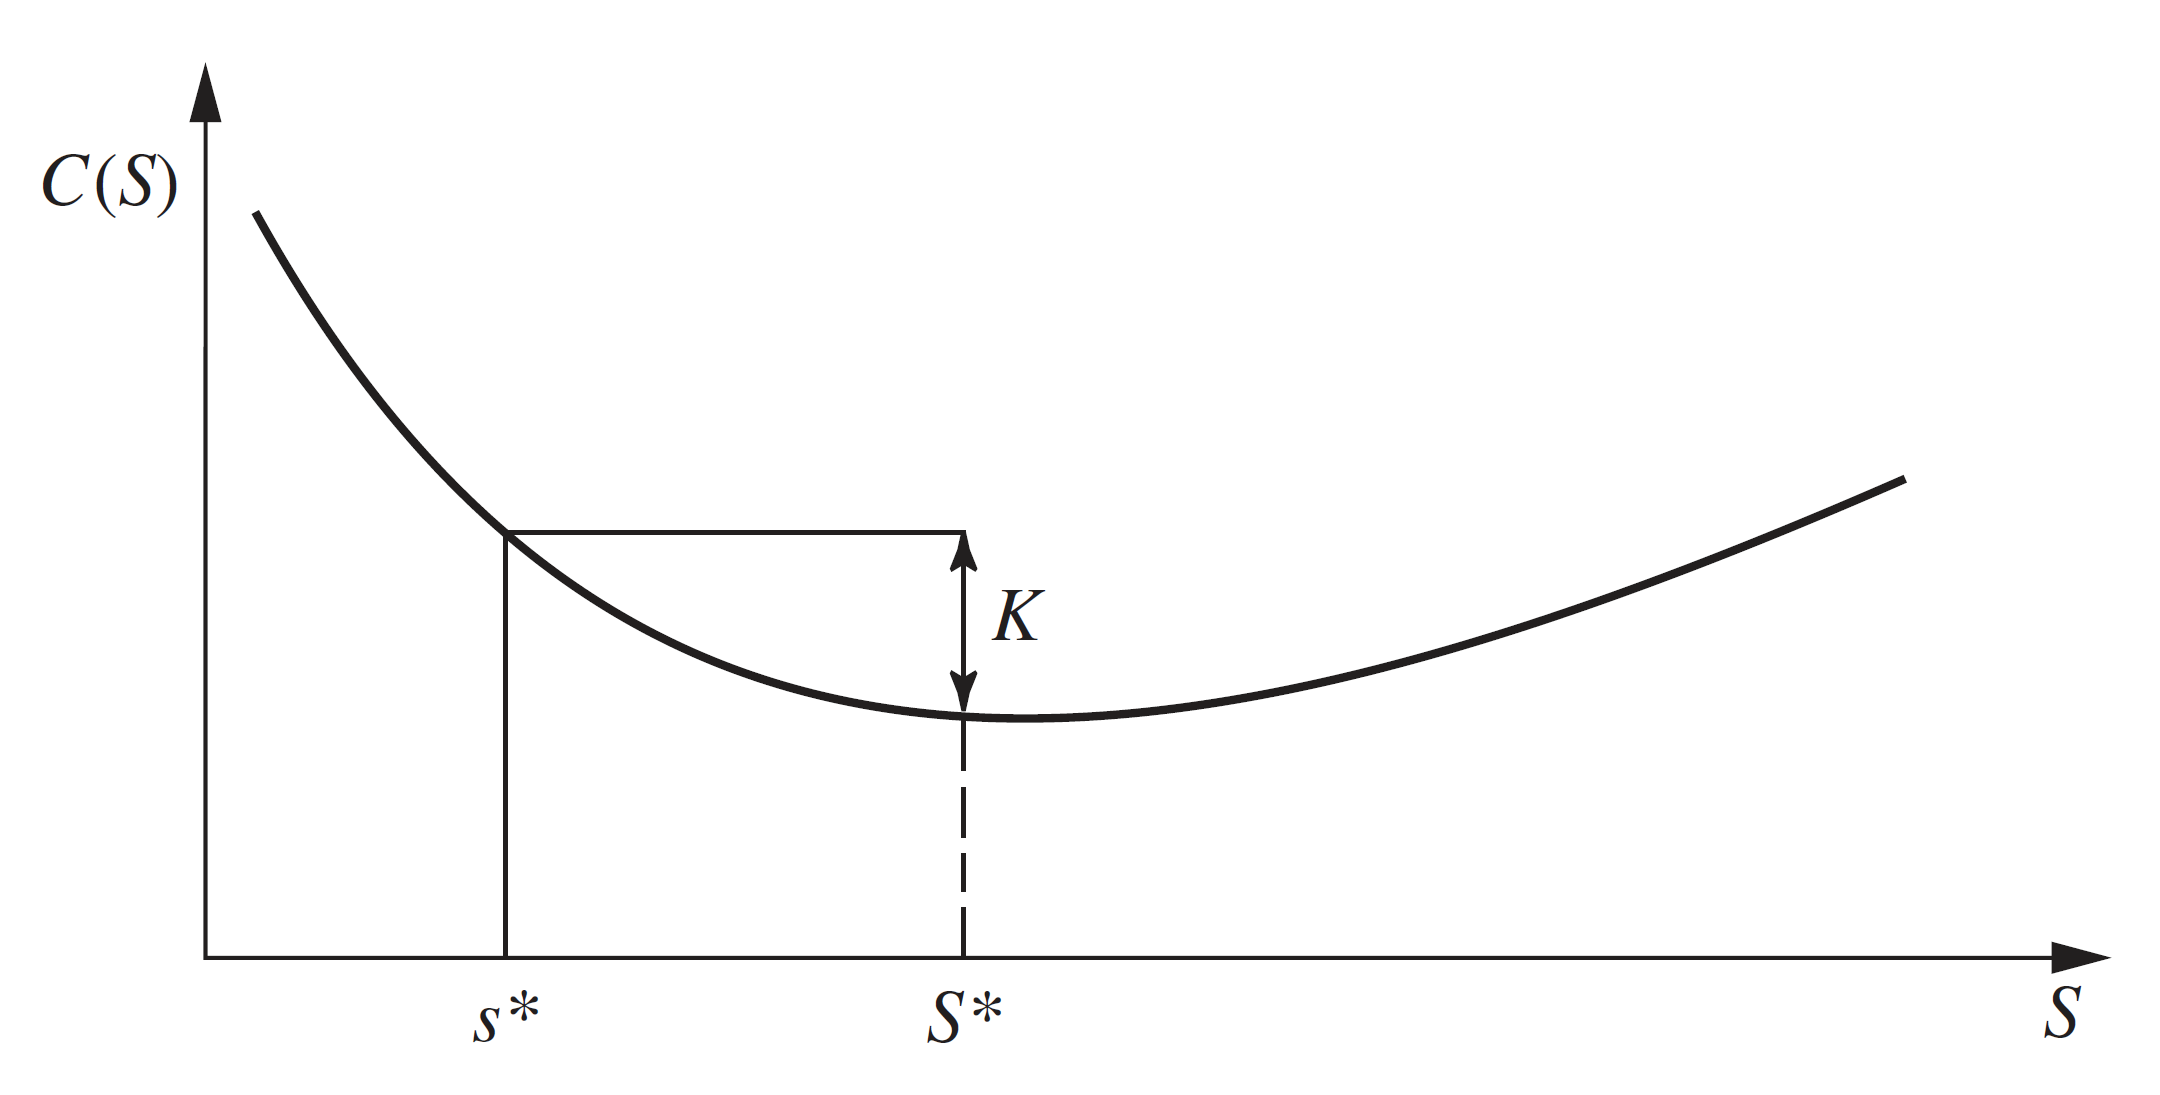
\includegraphics[width= 1\linewidth]{10}
		\caption{\small\textit{\color{toanhocdoisong}Hình $9$. Cách tìm $s^*$ khi có $S^*$.}}
		\vspace*{-10pt}
	\end{figure}
	Ta hãy xét một giá trị $s^*<S^*$ sao cho $C(s^* )=K+C(S^*)$ (giá trị $s^*>S*$ không có ý nghĩa về mặt thực tế). Trong một bài toán cụ thể, nếu đã biết được dạng của $f(x), s^*$ là hoàn toàn xác định được. 
	\vskip 0.1cm
	Phương án của ta cho trường hợp $I>0,K>0$ sẽ như sau:
	\vskip 0.1cm
	Nếu $I<s^*$ thì $C(S^* )<K+C(I)$ và ta đặt hàng với lượng hàng bằng $S^*$.
	\vskip 0.1cm
	Nếu $I \ge s^*$ thì $C(S) \le K+C(I)$ với mọi $S \ge I$ do đó ta không đặt hàng.
	\vskip 0.1cm
	$\pmb{5.}$ \textbf{\color{toanhocdoisong}Lời kết}
	\vskip 0.1cm
	Trong bài viết này, chúng ta đã thấy sự đa dạng của các bài toán có sử dụng mô hình EOQ cũng như việc ứng dụng các kỹ thuật đa dạng tìm cực trị của hàm số để cho ra nghiệm tối ưu. Các bài toán cực trị còn rất nhiều ứng dụng khác trong đời sống mà Pi sẽ trình bày với độc giả trong những số sau này.
	\vskip 0.1cm
	\textbf{\color{toanhocdoisong}Phụ lục:} Đạo hàm của tích phân có cận phụ thuộc tham biến
	\vskip 0.1cm
	Xét tích phân $I(t) = \int_{\alpha(t)}^{\beta(t)}{f(x)dx}$ với $ \alpha(t)$ và  $\beta(t)$ là các hàm khả vi theo $t$. Giả sử rằng khi $t \in [c,d]$ thì  $\alpha(t)$ và  $\beta(t)$ nhận giá trị trong $[a,b]$.
	\vskip 0.1cm
	Xét $t_0 \in [c,d]$, ta có:
	\begin{align*}
		I(t) =& \int_{\alpha(t)}^{\alpha(t_0)}{f(x)dx} + \int_{\alpha(t_0)}^{\beta(t_0)}{f(x)dx} \\
		&+ \int_{\beta(t_0)}^{\beta(t)}{f(x)dx}\\
		=& I_1(t) + I_2 + I_3(t).
	\end{align*}
	Do $I_2$ không phụ thuộc $t$ nên:
	\begin{align*}
		I'(t_0) = I_1'(t_0) + I_3'(t_0).
	\end{align*}
	Theo định nghĩa đạo hàm:
	\begin{align*}
		&I_3'(t_0)= \mathop {\lim }\limits_{t \to {t_0}} \frac{{{I_3}(t) - {I_3}({t_0})}}{{t - {t_0}}} \\
		= &\mathop {\lim }\limits_{t \to {t_0}} \frac{1}{{t \!-\! {t_0}}}\!\!\left[ \int_{\beta ({t_0})}^{\beta (t)} {f(x)dx}  \!-\! \int_{\beta ({t_0})}^{\beta ({t_0})} {f(x)dx}  \right] \\
		= &\mathop {\lim }\limits_{t \to {t_0}} \frac{1}{{t - {t_0}}}\int_{\beta ({t_0})}^{\beta (t)} {f(x)dx}
	\end{align*}
	Đến đây, ta cần dùng định lý giá trị trung bình cho tích phân: với hàm số $f(x)$ liên tục trên $[a,b]$, tồn tại giá trị $\xi \in [a,b]$ sao cho $\int_a^b{f(x)dx} = (b-a)f(\xi)$. Thật vậy, xét hàm số $f(x)$ liên tục trong khoảng $[a,b]$, khi đó tồn tại giá trị $m$ và $M$ sao cho $m \le f(x) \le M$ với mọi $x$ trong khoảng trên. Do đó:
	\begin{align*}
		\int_a^b{mdx} \le \int_a^b{f(x)dx} \le \int_a^b{Mdx},
	\end{align*}
	hay 
	\begin{align*}
		m(b-a) \le \int_a^b{f(x)dx} \le M (b-a).
	\end{align*}
	Việc này tương đương với: $\int_a^b{f(x)dx} = c(b-a), m \le c \le M$. Vì $f(x)$ là liên tục nên tồn tại giá trị $a \le \xi \le b$ sao cho $f(\xi)= c$ hay $\int_a^b{f(x)} = (b-a)f(\xi)$.
	\vskip 0.1cm
	Sử dụng định lý này cho biểu thức của $I_3'(t_0)$, ta có:
	\begin{align*}
		I_3'(t_0) &= \mathop {\lim }\limits_{t \to {t_0}} \frac{{\beta (t) - \beta ({t_0})}}{{t - {t_0}}}f(\xi ) \\
		&= \beta '({t_0})f\left( {\beta ({t_0})} \right).
	\end{align*}
	Tương tự:
	\begin{align*}
		I_1'(t_0) = - \alpha'(t_0)f\left(\alpha(t_0)\right).
	\end{align*}
	\textbf{\color{toanhocdoisong}Tài liệu tham khảo}
	\vskip 0.1cm
	[$1$] Erlenkotter, D. ($1990$). Ford Whitman Harris and the Economic Order Quantity Model. \textit{Operations Research}, $38(6)$, $937-946$. \url{https://www.jstor.org/stable/170961}
	\vskip 0.1cm
	[$2$] Hillier, F. S., \& Lieberman, G. J. ($2015$). \textit{Introduction to operations research}. Mcgraw--Hill.
	\vskip 0.1cm
	[$3$] Taha, H. A. ($2017$). \textit{Operations research: an introduction}. Pearson Education Limited.
\end{multicols}
	\newpage

	\setcounter{figure}{0}
	\thispagestyle{duongvaotoanhocnone}
\pagestyle{duongvaotoanhoc}
\everymath{\color{duongvaotoanhoc}}
\graphicspath{{../duongvaotoanhoc/pic/}}
\blfootnote{$^1$\color{duongvaotoanhoc}Universit\'e Paris--Saclay.}
\begingroup
\AddToShipoutPicture*{\put(0,616){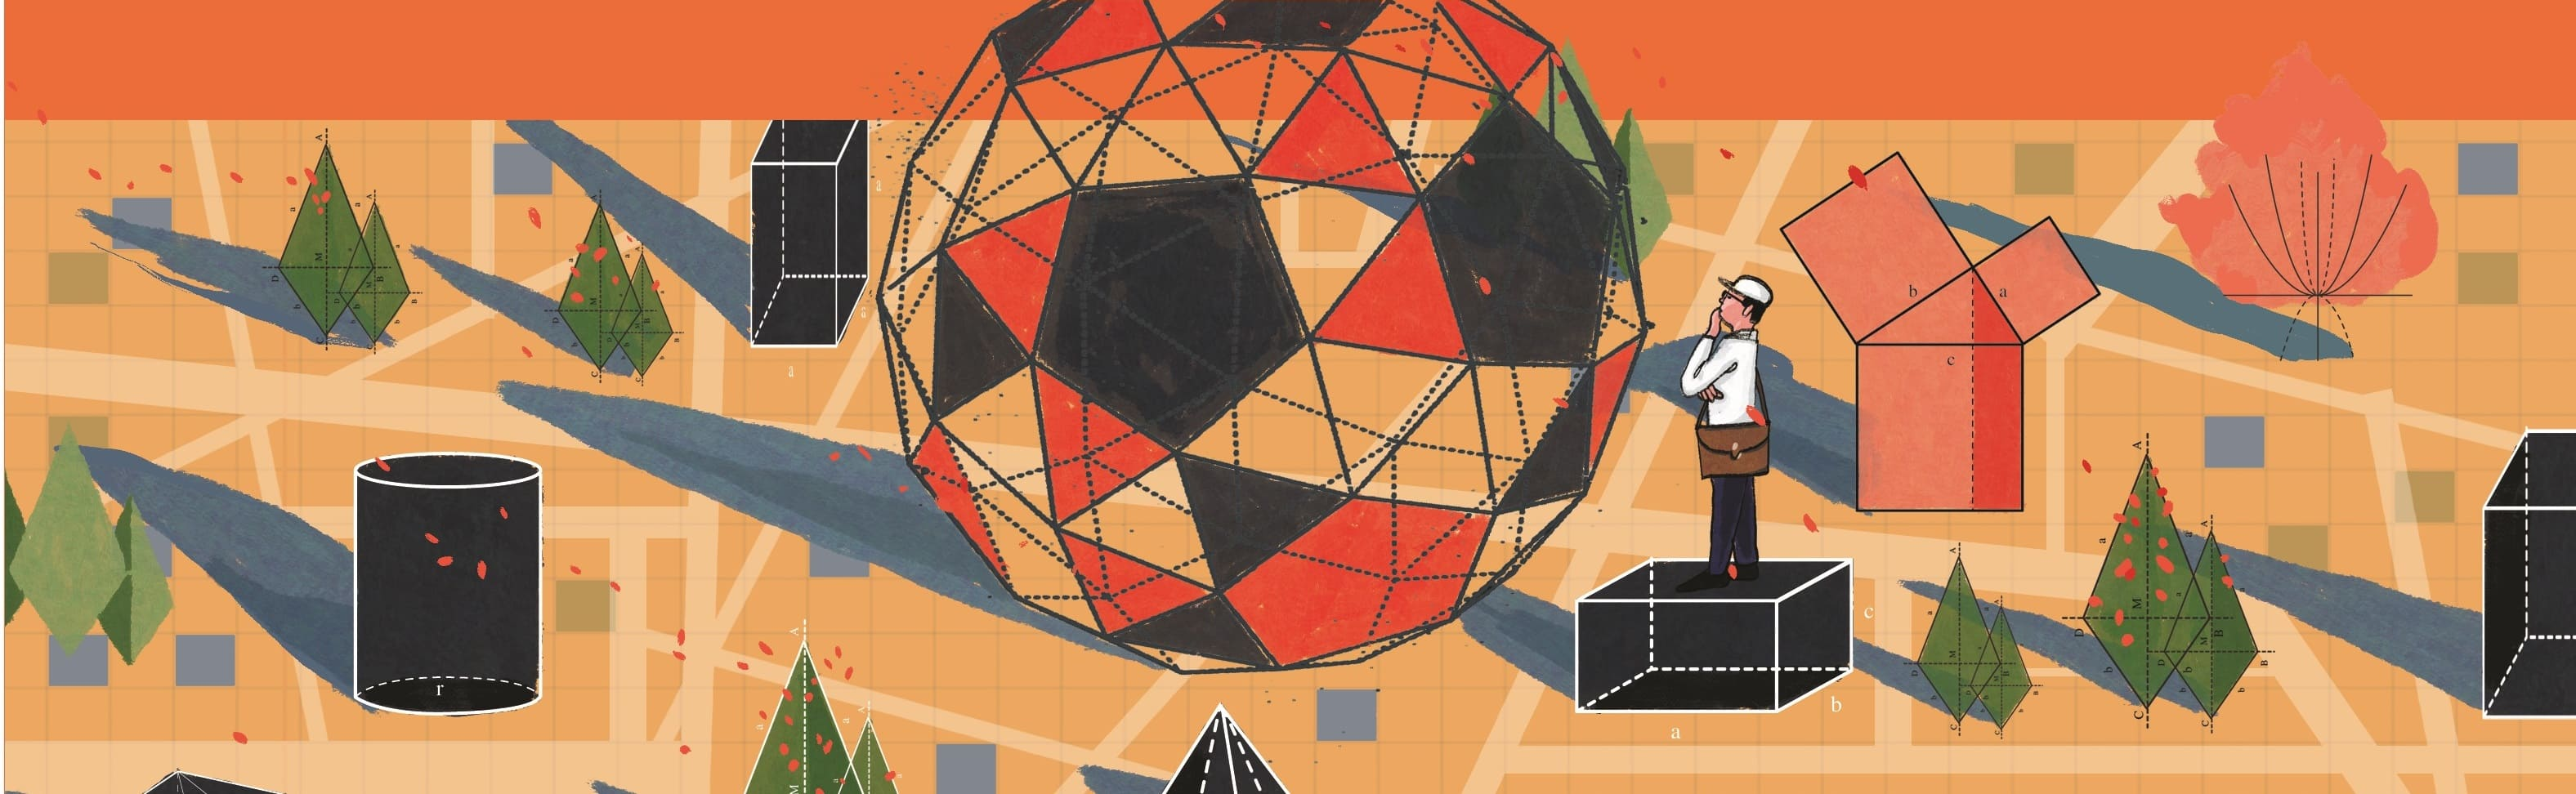
\includegraphics[width=19.3cm]{../bannerduongvao}}}
\AddToShipoutPicture*{\put(58,522){
\includegraphics[scale=1]{../tieude.pdf}}}
\centering
\endgroup
\vspace*{185pt}

\begin{multicols}{2}	
	\textbf{\color{duongvaotoanhoc}Lược đồ}
	\vskip 0.1cm
	Bây giờ, hãy dạo qua thế giới hình học đại số một chút. Với ý tưởng tiên phong của Descartes là nghiên cứu các đối tượng hình học bằng các hệ tọa độ và phương trình đa thức, người ta đã dần dần phát triển hình học đại số. Khác với những người bạn bên tôpô học, các nhà hình học đại số nghiên cứu các đối tượng cứng nhắc hơn: tập nghiệm của các hệ phương trình đa thức. Sau một thời gian, giới toán học nhận ra rằng các trực giác hình học thường mang đến các chứng minh không chặt chẽ và đặc biệt là không giúp gì được ở số chiều cao hơn. Họ đã chuyển sang dùng đại số giao hoán làm công cụ chính để nghiên cứu hình học. Grothendieck, nhà toán học được công nhận rộng rãi là có ảnh hưởng nhất thế kỷ XX, đã cách mạng hóa hình học đại số một lần nữa bằng định nghĩa {\bf\color{duongvaotoanhoc} lược đồ}.
	\vskip 0.1cm
	Ta quay lại với khái niệm trường. Nếu bỏ qua việc luôn làm được phép chia, ta thu được khái niệm {\bf\color{duongvaotoanhoc} vành}. Chẳng hạn, $\mathbb{Z}$ và $\mathbb{Z}/n\mathbb{Z}$ là các vành (phép cộng và phép nhân được hiểu theo nghĩa hiển nhiên). Chú ý rằng ta vẫn yêu cầu làm được phép trừ, nên $\mathbb{N}$ không phải là một vành. Với mỗi vành $R$, ta xây dựng được một không gian tôpô $\text{Spec}(R)$, được gọi là {\bf\color{duongvaotoanhoc} phổ} của $R$. Nếu chỉ nhìn $\text{Spec}(R)$ như một không gian thì ta mất rất nhiều thông tin. Chẳng hạn, phổ của một trường luôn là một điểm. Vì thế, người ta đã làm giàu $\text{Spec}(R)$ bằng một cấu trúc gọi là {\bf\color{duongvaotoanhoc} bó}, chúng làm cho $\text{Spec}(R)$ trở thành một lược đồ.
	\begin{figure}[H]
		\vspace*{-5pt}
		\centering
		\captionsetup{labelformat= empty, justification=centering}
		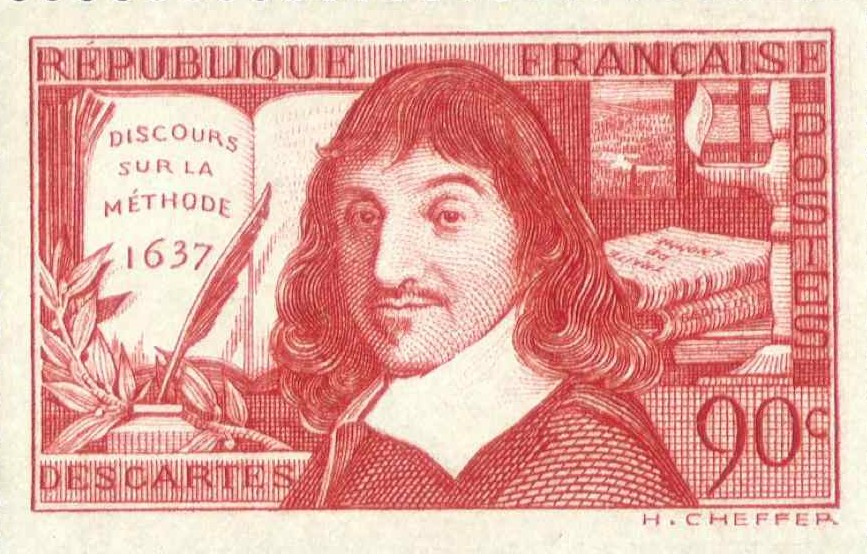
\includegraphics[width= 1\linewidth]{Descartes}
		\caption{\small\textit{\color{duongvaotoanhoc}Descartes trên tem thư Pháp.}}
		\vspace*{-10pt}
	\end{figure}
	Cũng như việc người ta quan tâm đến các hàm liên tục giữa các không gian tôpô, trong hình học đại số người ta quan tâm đến các {\bf\color{duongvaotoanhoc} cấu xạ} giữa các lược đồ. Một cấu xạ $\text{Spec}(R) \to \text{Spec}(S)$ đơn giản được cho bởi một {\bf\color{duongvaotoanhoc} đồng cấu vành} theo chiều ngược lại $f: S \to R$, đồng cấu ở đây nghĩa là $f(x+y) = f(x)+f(y)$, $f(xy) = f(x)f(y)$ và $f(1) = 1$. Chẳng hạn, $\mathbb{Z}$ là một vành con của $\mathbb{Q}$, và phép nhúng $\mathbb{Z} \to \mathbb{Q}$ cho ta một cấu xạ $\text{Spec}(\mathbb{Q}) \to \text{Spec}(\mathbb{Z})$. Về mặt tôpô thì $\text{Spec}(\mathbb{Q})$ chỉ có một điểm, nên ảnh của cấu xạ này là một điểm của $\text{Spec}(\mathbb{Z})$, được gọi là {\bf\color{duongvaotoanhoc} điểm tổng quát}. Với mỗi số nguyên tố $p$, phép lấy dư modulo $p: \mathbb{Z} \to \mathbb{F}_p$ cho ta một cấu xạ $\text{Spec}(\mathbb{F}_p) \to \text{Spec}(\mathbb{Z})$, đó là một {\bf\color{duongvaotoanhoc} điểm đóng}. Các điểm đóng này và điểm tổng quát tạo nên không gian $\text{Spec}(\mathbb{Z})$. Khác với các không gian Euclid, tôpô trên lược đồ $\text{Spec}(\mathbb{Z})$ rất thô: điểm tổng quát là một điểm nhưng lại trù mật trong cả không gian (người ta hay nói ``điểm tổng quát là điểm nằm ở mọi nơi, nhưng không nằm cụ thể ở đâu cả'').
	\begin{figure}[H]
		\vspace*{-5pt}
		\centering
		\captionsetup{labelformat= empty, justification=centering}
		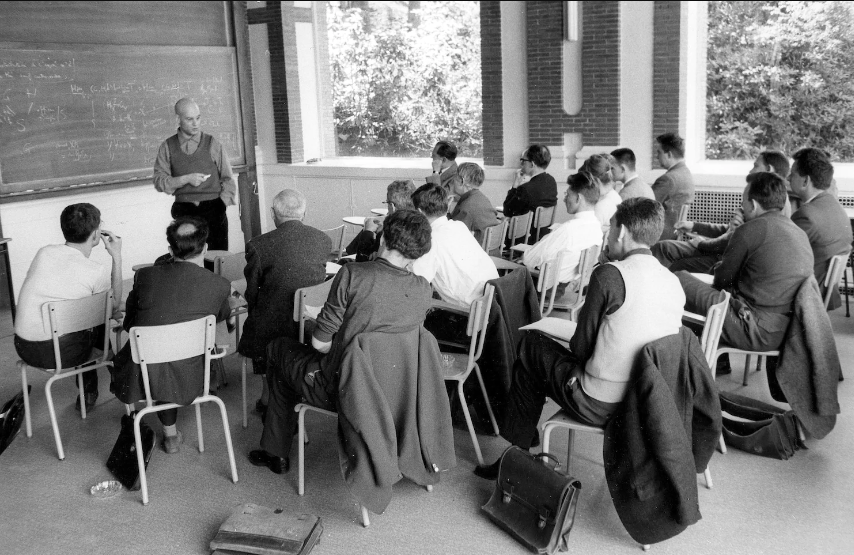
\includegraphics[width= 1\linewidth]{Grothendieck}
		\caption{\small\textit{\color{duongvaotoanhoc}Grothendieck giảng bài tại IHES $1962$.}}
		\vspace*{-10pt}
	\end{figure}
	Quay lại với lý thuyết không gian phủ. Khi áp dụng nó cho lược đồ, ta không thể chỉ xét khía cạnh tôpô ngây thơ được. Ta muốn $\text{Spec}(\mathbb{F}_p)$ giống với đường tròn $\mathbb{S}^1$, nhưng $\text{Spec}(\mathbb{F}_p)$ lại chỉ có một điểm. Vấn đề với không gian tôpô $\text{Spec}(R)$ là nó có quá ít lân cận, mỗi lân cận đều quá lớn. Cách khắc phục là sáng tạo ra một khái niệm tôpô mới dùng được cho các lược đồ (thứ mà ngày nay gọi là tôpô Grothendieck), với các ``lân cận'' mới. Một trong những loại tôpô đủ mạnh để phân biệt các ``không gian $1$ điểm'' $\text{Spec}(K)$ (với $K$ là các trường) là {\bf\color{duongvaotoanhoc} tôpô étale}. Từ ``étale'' được lấy từ văn học Pháp, mang nghĩa nôm na là trạng thái dịu dàng của biển. Với công cụ mới này, người ta định nghĩa được khái niệm nhóm cơ bản étale của lược đồ. Chẳng hạn, nhóm cơ bản étale của $\text{Spec}(\mathbb{F}_p)$ là một nhóm có cùng họ hàng với $\mathbb{Z}$, gọi là ``$\mathbb{Z}$ mũ''. Điều này giải thích vì sao việc coi $\text{Spec}(\mathbb{F}_p)$ như đường tròn $\mathbb{S}^1$ là hợp lý. Tương tự, khái niệm phủ trong thế giới lược đồ phải được hiểu là phủ étale. Đối với các trường, một phủ étale của $\text{Spec}(K)$ đơn giản là $\text{Spec}(L)$, với $L/K$ là một mở rộng bậc hữu hạn. Như vậy, dù $\text{Spec}(K)$ về mặt tôpô chỉ là $1$ điểm, nó lại có nhóm cơ bản étale không tầm thường, hay có rất nhiều phủ. 
	\vskip 0.1cm
	Thực ra khái niệm mở rộng trường và mở rộng vành còn cho ta thêm một chút bên phía tôpô, nó ứng với khái niệm {\bf\color{duongvaotoanhoc} phủ phân nhánh}. Nói nôm na, một phủ phân nhánh bậc $n$ là một hàm liên tục $p: Y \to X$ sao cho nếu bỏ đi một số hữu hạn điểm của $X$ (và các điểm của $Y$ nằm trên chúng) thì ta thu được một phủ $n$-tờ. Các điểm bỏ đi kia (cùng các điểm nằm trên) gọi là các {\bf\color{duongvaotoanhoc} điểm rẽ nhánh} của $p$. Hiện tượng rẽ nhánh là phiên bản hình học của hiện tượng ``nghiệm bội'' trong đại số. Ta xét ví dụ khi $Y$ là đường cong elliptic cho bởi phương trình $y^2=x(x-1)(x-2)$ trong $\mathbb{C}^2$ và $X = \mathbb{C}$. Lấy $p$ là phép chiếu lên trục hoành, $p(x,y) = x$. Khi bỏ đi các điểm $0, 1, 2$ khỏi $X$ (và các điểm $(0,0), (1,0), (2,0)$ khỏi $Y$), ta thu được một phủ $2$--tờ: với mỗi $x \neq 0,1,2$ thì phương trình $y^2=x(x-1)(x-2)$ có hai nghiệm phức phân biệt. Ở các điểm $0, 1, 2$ xảy ra hiện tượng rẽ nhánh, phương trình $y^2=0$ có nghiệm kép $y=0$. Ta nói rằng {\bf\color{duongvaotoanhoc} chỉ số rẽ nhánh} của $p$ tại các điểm $(0,0)$, $(1,0)$, $(2,0)$ bằng $2$.
	\vskip 0.1cm
	\textbf{\color{duongvaotoanhoc}Lý thuyết số đại số}
	\vskip 0.1cm
	Để tìm hiểu các phủ (étale) phân nhánh của lược đồ $\text{Spec}(\mathbb{Z})$, ta bắt đầu từ điểm tổng quát: Phủ étale của $\text{Spec}(\mathbb{Q})$ thì có dạng $\text{Spec}(K)$, với $K = \mathbb{Q}(\alpha)$, và $\alpha$ là nghiệm của một đa thức bậc $n$ bất khả quy với hệ số hữu tỷ. Số $\alpha$ như vậy được gọi là một {\bf\color{duongvaotoanhoc} số đại số}, chẳng hạn $\sqrt{2}, \sqrt[3]{2}, \frac{1 + \sqrt{-3}}{2}$ là các số đại số. Trường $K$ được gọi là một {\bf\color{duongvaotoanhoc} trường số}, và mọi phần tử của nó đều là số đại số. Ta muốn thứ gì đó trong $K$ đóng vai trò như các số nguyên đối với số hữu tỷ. Đó là các {\bf\color{duongvaotoanhoc} số nguyên đại số}. Chúng là những phần tử của $K$ mà là nghiệm của một đa thức với hệ số nguyên và hệ số đầu bằng $1$. Chẳng hạn $\sqrt{2}$ là một số nguyên đại số vì nó là nghiệm của $x^2 - 2$. Tương tự $\frac{1 + \sqrt{5}}{2}$ cũng là một số nguyên đại số (dù trông không có vẻ vậy) vì nó là nghiệm của $x^2-x-1$. Các số nguyên đại số trong $K$ tạo thành một vành $\mathcal{O}$. Việc chuyển từ $\mathbb{Z}$ sang $\mathcal{O}$ là chuyển từ lý thuyết số sơ cấp sang lý thuyết số đại số. Một bài tập đơn giản (bằng cách dùng phân tích duy nhất ra thừa số nguyên tố) là: Các số nguyên đại số trong $\mathbb{Q}$ chính là các số nguyên theo nghĩa cổ điển.
	\vskip 0.1cm
	Lý thuyết số đại số xuất phát từ nỗ lực chứng minh định lý lớn Fermat của Cauchy, Lamé,v.v. Ý tưởng như sau: với phương trình $x^2 + y^2 = z^2$ chẳng hạn, ta giải bằng cách đưa về $x^2=z^2-y^2=(z-y)(z+y)$, sau đó lập luận (với phân tích duy nhất ra thừa số nguyên tố) rằng $z-y$ và $z+y$ phải là các số chính phương. Bây giờ, xét phương trình $x^p+y^p=z^p$, với $p$ là số nguyên tố lẻ (dễ thấy ta chỉ cần xét trường hợp này). Để phân tích triệt để $z^p-y^p$ thành các nhân tử bậc nhất, ta buộc phải dùng căn bậc $p$ phức của $1$. Gọi nó là $\zeta = \cos(\frac{2\pi}{p})+i \cdot \sin(\frac{2\pi}{p})$. Thế thì $\zeta$ là một số nguyên đại số (nghiệm của phương trình $x^p - 1$). Và như vậy ta đưa về chứng minh rằng phương trình trên không có nghiệm trong vành mới $\mathbb{Z}[\zeta]$, vành các số nguyên đại số của $\mathbb{Q}(\zeta)$. Sơ hở của cách tiếp cận này là lập luận như trong trường hợp $p=2$ không còn đúng nữa, vì nói chung không có phân tích duy nhất ra thừa số nguyên tố trong $\mathbb{Z}[\zeta]$.
	\vskip 0.1cm
	Một ví dụ về sự không tồn tại của phân tích duy nhất là trường số $K = \mathbb{Q}(\sqrt{-5})$. Vành số nguyên đại số của nó là $\mathcal{O} = \mathbb{Z}[\sqrt{-5}]$, gồm các số có dạng $a+b\sqrt{-5}$ với $a,b \in \mathbb{Z}$. Số $6$ có thể phân tích thành $6 = 2 \cdot 3 = (1+\sqrt{-5}) \cdot (-\sqrt{-5})$. Để thấy rằng hai phân tích này là triệt để và thực sự khác nhau, ta định nghĩa {\bf\color{duongvaotoanhoc} chuẩn} của một số $a+b\sqrt{-5}$ bởi $N(a+b\sqrt{-5}) = a^2 + 5b^2$. Đây là một số tự nhiên, và ta thấy ngay rằng $N(xy) = N(x)N(y)$. Trong phân tích $6 = 2 \cdot 3 = (1+\sqrt{-5}) \cdot (-\sqrt{-5})$, ta có $N(2) = 4, N(3) = 9, N(1+\sqrt{-5}) = N(1-\sqrt{-5}) = 6$, nên các nhân tử xuất hiện ở hai phân tích thực sự khác nhau.  Ngoài ra, về cơ bản ta không thể phân tích thêm được nữa, vì không có phần tử nào có chuẩn bằng $2$ hoặc $3$ (một tính toán số học đơn giản cho thấy rằng các phương trình $a^2 + 5b^2 = 2$ và $a^2 + 5b^2 = 3$ đều không có nghiệm nguyên). Điều này cho thấy sự thiếu sót của phân tích duy nhất ra thừa số nguyên tố trong $\mathbb{Z}[\sqrt{-5}]$.
	\vskip 0.1cm
	Sự sụp đổ của phân tích duy nhất trong $\mathcal{O}$ đã chấm dứt hi vọng chứng minh định lý lớn Fermat bằng lý thuyết số đại số cổ điển. Dù vậy, vành $\mathcal{O}$ vẫn giữ được một tính chất của vành $\mathbb{Z}$; nó là một {\bf\color{duongvaotoanhoc} vành Dedekind}. Thay vì phân tích duy nhất của các số, người ta định nghĩa khái niệm {\bf\color{duongvaotoanhoc} số lý tưởng} (cái mà ngày nay gọi là {\bf\color{duongvaotoanhoc} iđêan}). Đại khái nó là thứ gì đó cho phép nói về quan hệ chia hết cũng như làm phép nhân. Việc $\mathcal{O}$ là vành Dedekind có nghĩa là mọi số lý tưởng đều phân tích một cách duy nhất ra các số lý tưởng nguyên tố. Một số nguyên đại số $a \in \mathcal{O}$ định nghĩa một số lý tưởng $(a)$, được gọi là một số lý tưởng chính. Hai số $a$ và $b$ định nghĩa cùng một số lý tưởng nếu chúng {\bf\color{duongvaotoanhoc} liên kết}, nghĩa là $a|b$ đồng thời $b|a$. Nói riêng, nếu $u|1$ thì $(u) = (1)$. Nếu tất cả số lý tưởng nguyên tố đều có dạng trên thì $\mathcal{O}$ có phân tích duy nhất của các số (thực sự). Điều này không đúng trong $\mathbb{Z}[\sqrt{-5}]$; cụ thể là khi phân tích $(6) = (2) \cdot (3) = (1 + \sqrt{-5}) \cdot (1 - \sqrt{-5})$, ta vẫn phân tích được tiếp: $(2) = \mathfrak{p}_1\mathfrak{p}_2$, $(3) = \mathfrak{p}_3\mathfrak{p}_4$, $(1 + \sqrt{-5}) = \mathfrak{p}_1\mathfrak{p}_3$, $(1 - \sqrt{-5}) = \mathfrak{p}_2\mathfrak{p}_4$, trong đó $\mathfrak{p}_1, \mathfrak{p}_2, \mathfrak{p}_3, \mathfrak{p}_4$ là các số lý tưởng nguyên tố {\it không chính}. Chuẩn của chúng lần lượt là $N(\mathfrak{p}_1) = N(\mathfrak{p}_2) = 2$ và $N(\mathfrak{p}_3) = N(\mathfrak{p}_4) = 3$. Như vậy ta có phân tích duy nhất của $(6)$ thành các số lý tưởng.
	\vskip 0.1cm
	Cũng như mỗi số nguyên tố $p$ ứng với các điểm đóng $\text{Spec}(\mathbb{F}_p) \to \text{Spec}(\mathbb{Z})$, mỗi số lý tưởng nguyên tố $\mathfrak{p}$ trong trong $\mathcal{O}$ cho ta một trường hữu hạn $\mathbb{F}_{\mathfrak{p}}$ (gọi là {\bf\color{duongvaotoanhoc} trường thặng dư} của $\mathfrak{p}$), cùng một điểm đóng $\text{Spec}(\mathbb{F}_{\mathfrak{p}}) \to \text{Spec}(\mathcal{O})$. Cùng với điểm tổng quát $\text{Spec}(K)$, chúng tạo thành lược đồ $\text{Spec}(\mathcal{O})$. Vì $\mathbb{Z}$ là một vành con của $\mathcal{O}$, ta có một cấu xạ $\text{Spec}(\mathcal{O}) \to \text{Spec}(\mathbb{Z})$, một phủ étale phân nhánh. Mỗi số nguyên tố $p$ trong $\mathbb{Z}$ có thể không còn là số lý tưởng nguyên tố trong $\mathcal{O}$, nó phân rã thành tích của một số hữu hạn số lý tưởng nguyên tố, $(p) = \mathfrak{p_1}\mathfrak{p_2}\cdots\mathfrak{p_n}$. Các số lý tưởng nguyên tố xuất hiện trong phân tích trên chính xác là những điểm của $\text{Spec}(\mathcal{O})$ nằm trên điểm đóng của $\text{Spec}(\mathbb{Z})$ ứng với $p$. Hiện tượng phân nhánh nhánh xảy ra nếu có một số lý tưởng $\mathfrak{p}_i$ xuất hiện nhiều lần trong phân tích trên, ta gọi đó số lần đó là {\bf\color{duongvaotoanhoc} chỉ số rẽ nhánh} của $\mathfrak{p}_i$, nó đóng vai trò như chỉ số rẽ nhánh trong tôpô cổ điển.
	\begin{figure}[H]
		\vspace*{-5pt}
		\centering
		\captionsetup{labelformat= empty, justification=centering}
		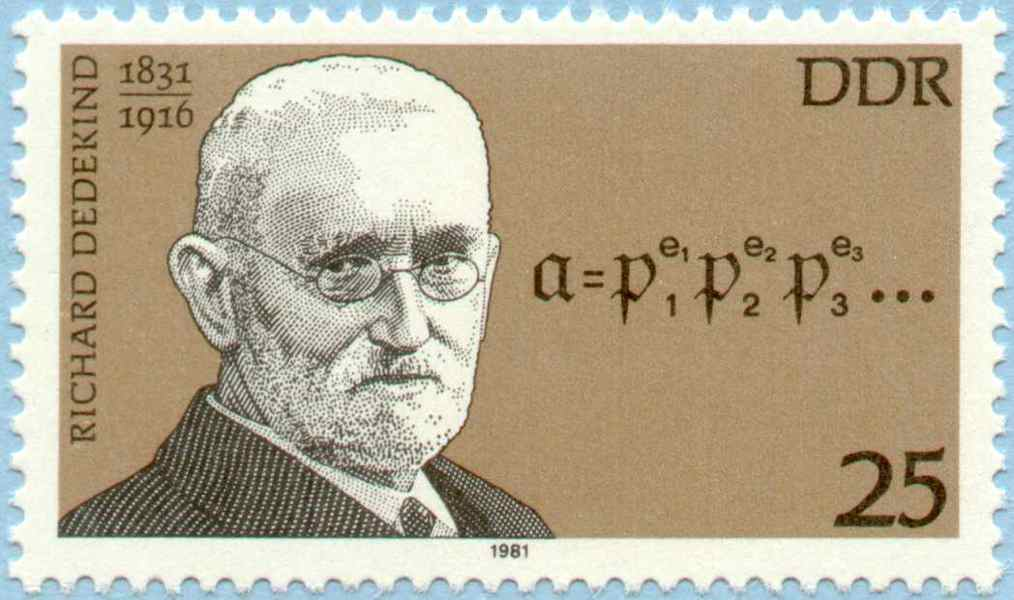
\includegraphics[width= 1\linewidth]{Dedekind}
		\caption{\small\textit{\color{duongvaotoanhoc}Dedekind trên tem thư CHDC Đức.}}
		\vspace*{-10pt}
	\end{figure}
	Một bất đẳng thức trong lý thuyết số đại số, {\it chặn Minkowski}, cho phép xác định cụ thể phân tích trên. Hơn thế nữa, nó còn cho ta biết chính xác khi nào thì một số nguyên tố $p$ rẽ nhánh trong $\mathcal{O}$. Một hệ quả của nó là với mọi trường số $K$, luôn có ít nhất một số nguyên tố $p$ rẽ nhánh trong vành $\mathcal{O}$ các số nguyên đại số trong $K$, nghĩa là $\text{Spec}(\mathbb{Z})$ không có phủ  étale không rẽ nhánh nào ngoài phủ tầm thường (cho bởi ánh xạ đồng nhất $\mathbb{Z} \to \mathbb{Z}$), hay nó là đơn liên.
	\vskip 0.1cm
	\textbf{\color{duongvaotoanhoc}Nút}
	\vskip 0.1cm
	Trong thế giới của các không gian tôpô thì có rất nhiều không gian đơn liên, và ta muốn tìm cái nào giống với $\text{Spec}(\mathbb{Z})$. Sự đột phá nằm ở các phát hiện sau đây của Mumford, Manin, và sau này là Mazur. Ở phía tôpô, các khái niệm điểm ($0$--chiều), đường ($1$--chiều), mặt ($2$--chiều) được tổng quát lên thành các đa tạp. Một đa tạp $3$--chiều là một không gian tôpô mà nhìn địa phương thì giống như không gian Euclid $\mathbb{R}^3$ (cũng như bề mặt Trái Đất là một đa tạp $2$--chiều, nhìn địa phương thì giống như mặt phẳng).
	\vskip 0.1cm
	Bên cạnh nhóm cơ bản, tôpô đại số cổ điển còn cung cấp các bất biến đại số khác cho các không gian tôpô, gọi là các {\bf\color{duongvaotoanhoc} nhóm đồng điều}. Nhóm đồng điều bậc $n$ của một đa tạp $X$ được xây dựng như sau: Xét các tổ hợp tạo thành từ một số đa tạp con $n$--chiều (chúng được gọi là các {\bf\color{duongvaotoanhoc} $n$-dây chuyền}). Nếu chúng tạo thành một vòng kín, ta gọi nó là một {\bf\color{duongvaotoanhoc} $n$--chu trình}. Nếu nó tạo thành biên của một đa tạp con $(n+1)$--chiều, ta gọi nó là một {\bf\color{duongvaotoanhoc} $n$--biên}. Một $n$--biên thì luôn là một $n$--chu trình. Nhóm $H_n(X)$ được định nghĩa là chênh lệch giữa các nhóm các $n$--chu trình và nhóm các $n$--biên: một $n$--chu trình mà không phải $n$--biên thì nó bao quanh một ``lỗ thủng'' $(n+1)$--chiều; như vậy các nhóm đồng điều phát hiện các lỗ thủng trên $X$. Phiên bản đối ngẫu của đồng điều là {\bf\color{duongvaotoanhoc} đối đồng điều}, các nhóm $H^n(X)$. Về cơ bản thì chúng cũng phát hiện các lỗ thủng. Về mặt kỹ thuật thì chúng dễ tính toán hơn đồng điều một chút, đồng thời có nhiều cấu trúc hơn. {\it Đối ngẫu Poincaré} nói rằng nếu $X$ là một đa tạp đóng, khả định hướng, $d$--chiều, thì ta có một đối ngẫu hoàn hảo giữa hai nhóm $H^{d-i}(X)$ và $H^i(X)$ với mỗi $i = 0,1,\ldots,d$.
	\vskip 0.1cm
	Với các lược đồ, các nhóm đối đồng điều nhìn chung không cho thông tin gì (phần lớn chúng bằng $0$) khi ta tính theo tôpô thông thường. Một lần nữa nhờ công của Grothendieck, ta có thể tính {\bf\color{duongvaotoanhoc}đối đồng điều étale}.  Trên một trường, chúng được gọi là {\bf\color{duongvaotoanhoc}đối đồng điều Galois}, một công cụ đã được dùng từ lâu trước đó trong số học. Với các trường hữu hạn, đối đồng điều Galois của chúng rất đơn giản, chúng khác $0$ ngoài bậc $0$ và $1$, và ta có một đối ngẫu hoàn hảo giữa các nhóm đối đồng điều ở hai bậc này. Điều này tương tự với đối ngẫu Poincaré cho các đa tạp $1$--chiều, khẳng định thêm niềm tin rằng phổ của trường hữu hạn là phiên bản đại số của đường tròn. 
	\vskip 0.1cm
	Đối với các lược đồ $\text{Spec}(\mathcal{O})$, với $\mathcal{O}$ là vành số nguyên đại số của một trường số $K$ nào đó, các nhóm đối đồng điều étale thỏa mãn đối ngẫu giữa bậc $0$ và bậc $3$ cũng như bậc $1$ và bậc $2$. Các kết quả này được gọi là {\it đối ngẫu Artin--Verdier}, được khám phá khi áp dụng đối đồng điều étale cho lý thuyết trường các lớp toàn cục, một phần của lý thuyết số. Điều này gợi cho ta rằng phiên bản tôpô của $\text{Spec}(\mathcal{O})$ ``nên" là các đa tạp $3$--chiều. Vậy $\text{Spec}(\mathbb{Z})$ ứng với đa đạp đóng $3$--chiều nào? Ta thấy ở trên rằng $\text{Spec}(\mathbb{Z})$ đơn liên, và đa tạp đóng $3$--chiều đơn liên thì chỉ có thể đồng phôi với mặt (siêu) cầu  $\mathbb{S}^3$! Đó là nội dung của {\it giả thuyết Poincaré}, bài toán duy nhất đã được giải trong $7$ bài toán thiên niên kỷ. Tác giả của lời giải, thiên tài lập dị Perelman, đã từ chối cả Huy chương Fields lẫn Giải thưởng Thiên niên kỷ (Millennium Prize) cho công trình vô song của mình.
	\vskip 0.1cm
	Sau khi bỏ ra rất nhiều công sức, ta đã thấy được cầu nối mong manh giữa tôpô học và số học, rằng phiên bản số học của $\mathbb{S}^1$ là (phổ của) một trường hữu hạn, và của một đa tạp đóng $3$--chiều là vành các số nguyên đại số của một trường số. Bây giờ là lúc chúng ta thu hoạch kết quả, chiêm ngưỡng những sự tương tự đáng ngạc nhiên dựa trên cầu nối này. Một số lý tưởng nguyên tố $\mathfrak{p}$ trong $\mathcal{O}$ cho ta một phép nhúng $\text{Spec}(\mathbb{F}_\mathfrak{p}) \hookrightarrow \text{Spec}(\mathcal{O})$. Về phía tôpô, ta xét các phép nhúng $\mathbb{S}^1 \hookrightarrow M$, với $M$ là một đa tạp (đóng, khả định hướng) $3$-chiều. Chúng được gọi là các {\bf\color{duongvaotoanhoc} nút} trong $M$. Nói riêng, phiên bản tôpô của mỗi số nguyên tố $p$ (với phép nhúng tương ứng $\text{Spec}(\mathbb{F}_p) \hookrightarrow \text{Spec}(\mathbb{Z})$) là một nút trong $\mathbb{S}^3$ (ta sẽ tập trung vào các nút này). Từ một định lý sâu sắc trong tôpô học, {\it định lý Borsuk--Ulam}, ta có thể chỉ ra rằng một phép nhúng như thế không thể là toàn ánh, nghĩa là ta có thể xem một nút như một phép nhúng từ $\mathbb{S}^1$ vào $\mathbb{S}^3$ bỏ đi một điểm, nói cách khác chính là không gian Euclid $\mathbb{R}^3$.
	\vskip 0.1cm
	Để biểu diễn một nút $K: \mathbb{S}^1 \hookrightarrow \mathbb{R}^3$ ta có thể chiếu nó lên một mặt phẳng sao cho tại mỗi điểm giao nhau chỉ có đúng $2$ đường đi qua. Chúng ứng với một {\bf\color{duongvaotoanhoc} sợi trên} và một {\bf\color{duongvaotoanhoc} sợi dưới}, ta biểu diễn sợi dưới bằng nét đứt tại giao điểm đó.  Đó là một {\bf\color{duongvaotoanhoc} biểu đồ phẳng} của nút.
	\begin{figure}[H]
		\vspace*{-5pt}
		\centering
		\captionsetup{labelformat= empty, justification=centering}
		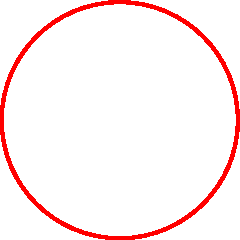
\includegraphics[width= 0.29\linewidth]{unknot.pdf}\quad
		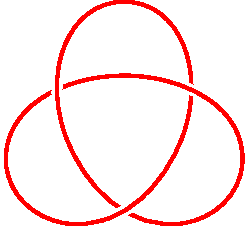
\includegraphics[width= 0.29\linewidth]{trefoil.pdf}\quad
		
\includegraphics[width= 0.29\linewidth]{figure 8.pdf}
		\caption{\small\textit{\color{duongvaotoanhoc}Hình $10$: Biểu đồ phẳng của nút tầm thường, nút ba lá, và nút số $8$.}}
		\vspace*{-10pt}
	\end{figure}
	Tất nhiên, mọi nút đều đồng phôi với $\mathbb{S}^1$. Ta cần cả thông tin về phép nhúng $\mathbb{S}^1 \to \mathbb{R}^3$ để phân biệt các nút với nhau. Các nhà lý thuyết nút gọi sự giống nhau của các nút là {\bf\color{duongvaotoanhoc} đẳng luân}. Một cách trực giác, hai nút đẳng luân nếu ta có thể tháo dỡ một nút rồi buộc thành nút còn lại (mà không cắt được cắt nút ra). Hóa ra, hai nút đẳng luân khi và chỉ khi phần bù của chúng trong $\mathbb{S}^3$ đồng phôi với nhau ({\it định lý Gordon--Luecke}).
	\vskip 0.1cm
	\textbf{\color{duongvaotoanhoc}Từ điển M$^2$KR}
	\vskip 0.1cm
	Từ điển Mazur--Morishita--Kapranov--Reznikov (M$^2$KR) là một danh sách những sự tương tự giữa lý thuyết số và hình học của các đa tạp $3$--chiều; ở đó các số lý tưởng tưởng ứng với các liên kết, các số lý tưởng nguyên tố ứng với các nút. Sau đây là một số tương ứng giữa tôpô và số học trong từ điển này.
	\vskip 0.1cm
	Mỗi số lý tưởng trong $\mathcal{O}$ phân tích thành tích của các số lý tưởng nguyên tố. Phiên bản tôpô của số lý tưởng là {\bf\color{duongvaotoanhoc} liên kết}: một liên kết trong một đa tạp đóng $3$--chiều $M$ là một phép nhúng từ một số hữu hạn bản sao rời rạc của $\mathbb{S}^1$ vào $M$. Các ví dụ về liên kết trong $\mathbb{S}^3$ là {\bf\color{duongvaotoanhoc} liên kết Hopf} và {\bf\color{duongvaotoanhoc} vòng Borromean}, lần lượt được tạo bởi $2$ và $3$ nút tầm thường lồng nhau.
	\begin{figure}[H]
		\vspace*{-15pt}
		\centering
		\captionsetup{labelformat= empty, justification=centering}
		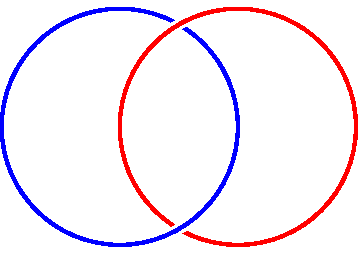
\includegraphics[width= 0.42\linewidth]{hopf.pdf}\quad\quad
		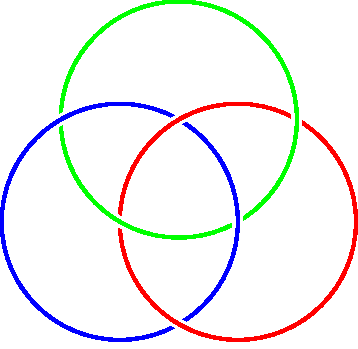
\includegraphics[width= 0.42\linewidth]{borromean.pdf}
		\caption{\small\textit{\color{duongvaotoanhoc}Hình $11$: Biểu đồ phẳng của liên kết Hopf và vòng Borromean.}}
		\vspace*{-10pt}
	\end{figure}
	Để thêm phần thuyết phục rằng tại sao $M$ lại tương ứng với (vành số nguyên đại số) một trường số, ta nhắc đến {\it định lý Alexander}: Mọi đa tạp đóng $3$--chiều đều là một phủ phân nhánh của $\mathbb{S}^3$, trong đó các điểm rẽ nhánh trong $\mathbb{S}^3$ tạo thành một liên kết. Tương tự, một mở rộng $L/K$ của trường số có thể được coi như một phủ phân nhánh giữa hai đa tạp đóng $3$--chiều.
	\begin{figure}[H]
		\vspace*{-5pt}
		\centering
		\captionsetup{labelformat= empty, justification=centering}
		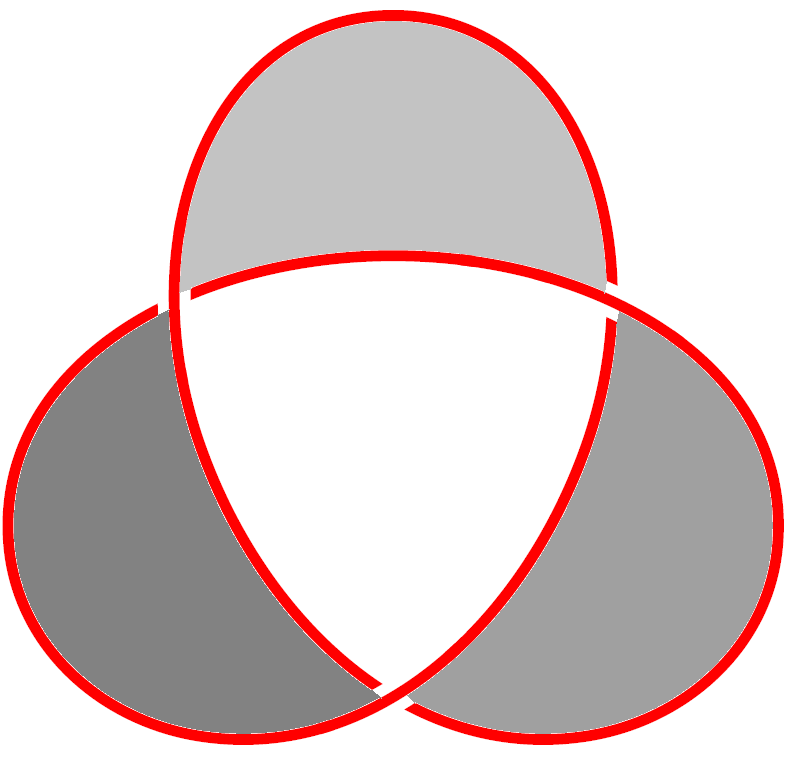
\includegraphics[width= 0.4\linewidth]{seifert1}\quad\quad
		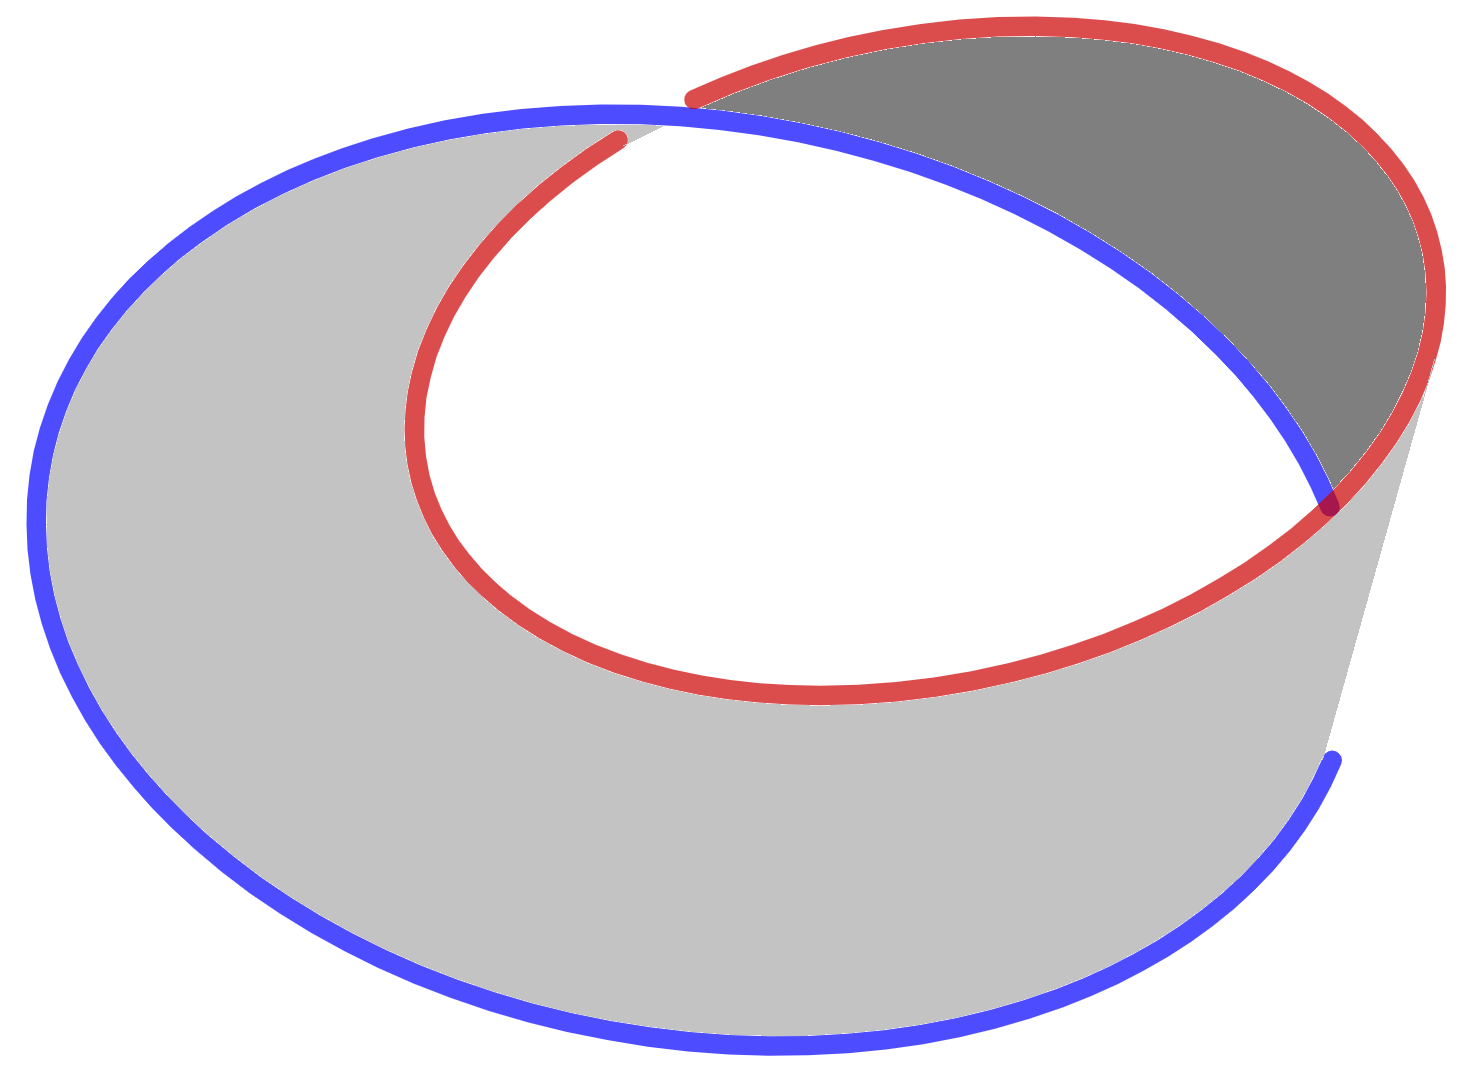
\includegraphics[width= 0.4\linewidth]{seifert2}
		\caption{\small\textit{\color{duongvaotoanhoc}Hình $12$: Mặt Seifert của nút ba lá và của liên kết Hopf (mặt M\"obius).}}
		\vspace*{-10pt}
	\end{figure}
	Một số nguyên đại số $a \in \mathcal{O}$ ứng với một mặt compact $S$ (có thể có biên) nhúng trong đa tạp đóng $3$--chiều $M$. Số lý tưởng chính $(a)$ ứng với biên $\partial S$, đây là một liên kết, và chúng ứng với các $1$--đối biên, tức là phần tử $0$ trong nhóm đồng điều $H_1(M)$. Các số lý tưởng khác tương ứng với các liên kết, chúng là các $1$--chu trình mà không phải biên, đại diện cho các phần tử không tầm thường của $H_1(M)$. Ta biết rằng trong $\mathbb{Z}$ có phân tích duy nhất ra thừa số nguyên tố, hay mọi số lý tưởng nguyên tố đều là số lý tưởng chính. Tương ứng, với $M = \mathbb{S}^3$, ta có $H_1(M) = 0$ (vì $\mathbb{S}^3$ không có lỗ thủng $2$--chiều nào), nghĩa là mọi liên kết đều là biên của một mặt nào đó. Seifert đã đưa ra một thuật toán khá đơn giản để xây dựng một mặt với biên cho trước. Chẳng hạn, {\bf\color{duongvaotoanhoc} mặt Seifert} của liên kết Hopf chính là {\it mặt M\"obius}.
	\vskip 0.1cm
	Sự tương tự tiếp theo: với $p$ là một số nguyên tố, ta xét vành $\mathbb{Z}_p$ các số nguyên $p$--adic cũng như trường $\mathbb{Q}_p$ các số $p$--adic. So với $\text{Spec}(\mathbb{Z})$, phổ $\text{Spec}(\mathbb{Z}_p)$ chỉ còn $2$ điểm là điểm tổng quát $\text{Spec}(\mathbb{Q}_p)$ và điểm đóng $\text{Spec}(\mathbb{F}_p)$, vì thế ta gọi thao tác này {\bf\color{duongvaotoanhoc} địa phương hóa} (tập trung nhìn vào số nguyên tố $p$ và quên đi các số nguyên tố khác). Thao tác này ứng với việc lấy {\bf\color{duongvaotoanhoc} lân cận ống} $V$ của nút, kết quả thu được là một hình xuyến đặc. Dù hình xuyến đặc không đồng phôi với đường tròn, chúng {\bf\color{duongvaotoanhoc} tương đương đồng luân với nhau}, điều này ứng với việc $\text{Spec}(\mathbb{Z}_p)$ và $\text{Spec}(\mathbb{F}_p)$ {\bf\color{duongvaotoanhoc} tương đương đồng luân étale với nhau}. Khi bỏ nút ban đầu khỏi $V$, ta thu được một không gian tương đương đồng luân với mặt xuyến (rỗng). Nhóm cơ bản của mặt xuyến là $\mathbb{Z} \times \mathbb{Z}$, một nhóm được sinh bởi hai phần tử là hai khuyên như trong Hình $13$.
	\begin{figure}[H]
		\vspace*{-5pt}
		\centering
		\captionsetup{labelformat= empty, justification=centering}
		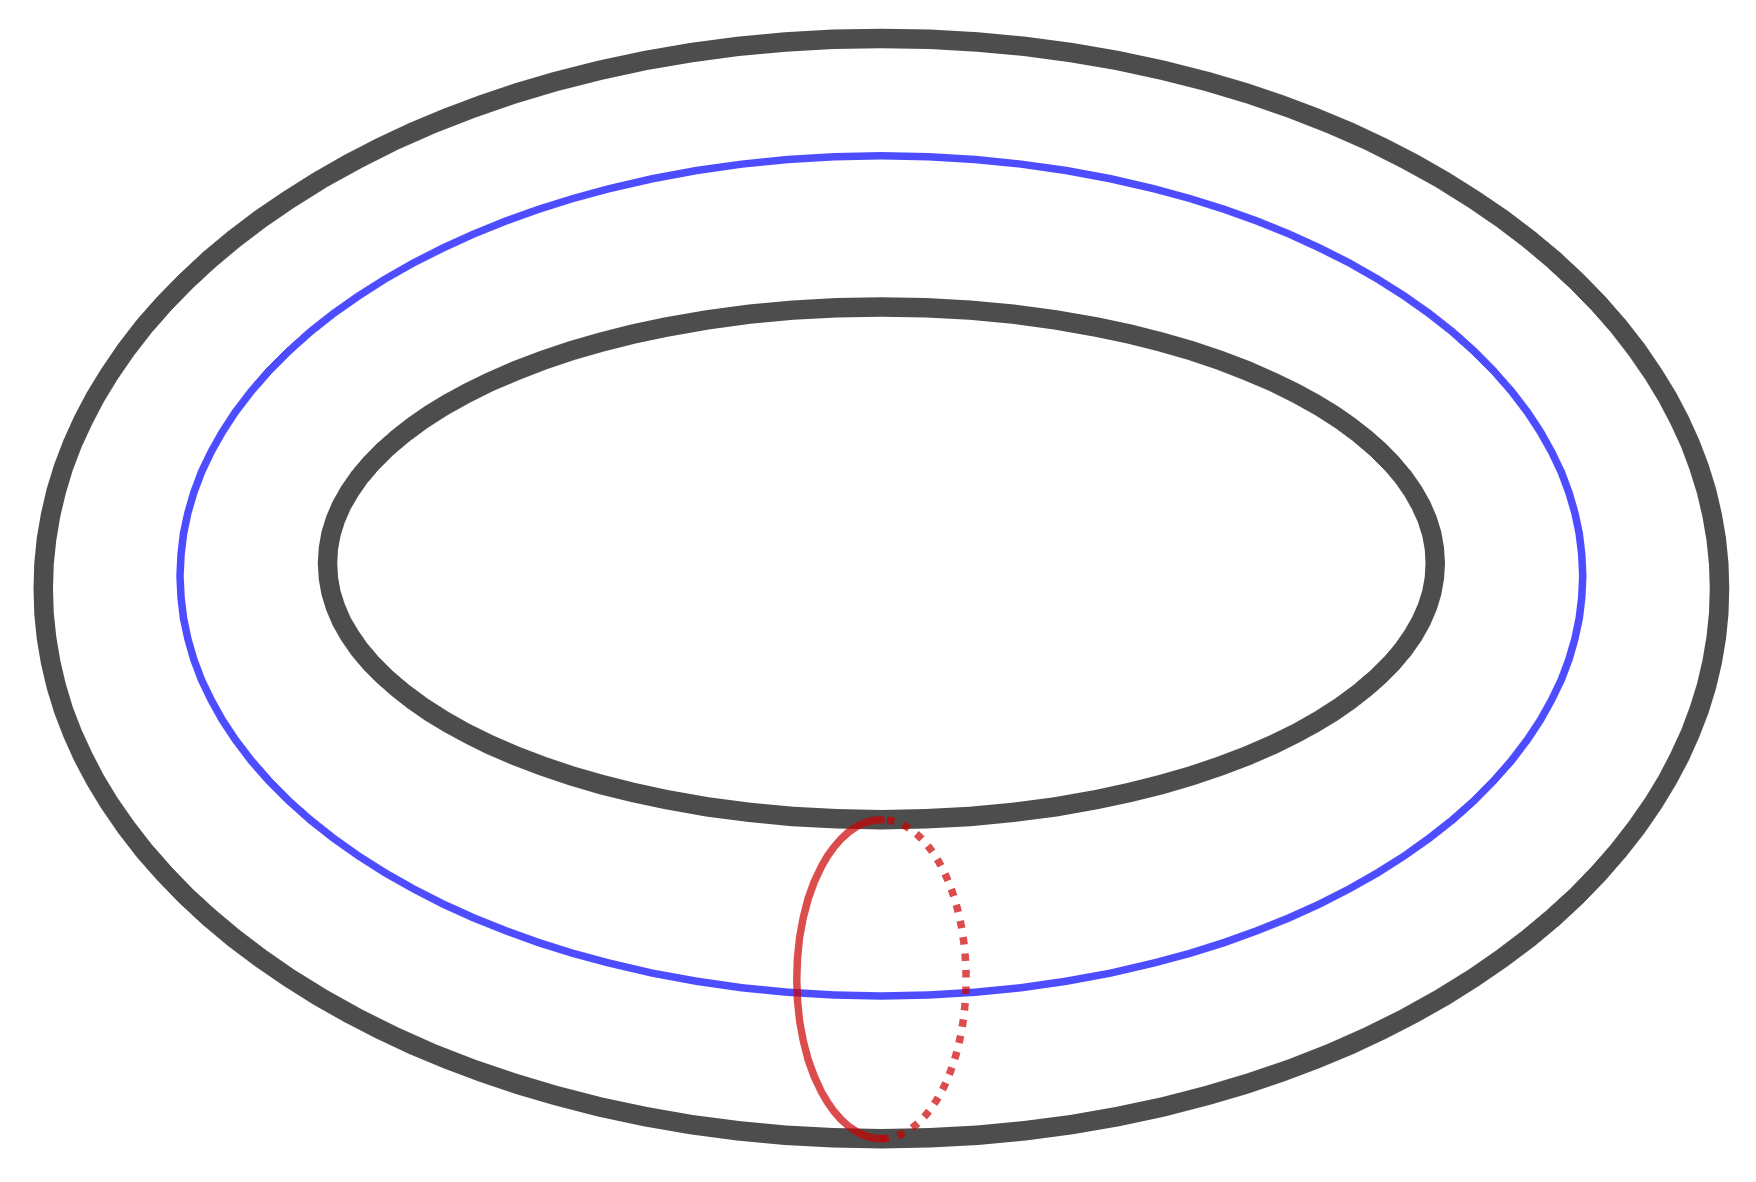
\includegraphics[width= 0.7\linewidth]{h13}
		\caption{\small\textit{\color{duongvaotoanhoc}Hình $13$: Nhóm cơ bản của mặt xuyến được sinh bởi hai khuyên màu xanh và màu đỏ.}}
		\vspace*{-5pt}
	\end{figure}
	Tương ứng, khi bỏ $\text{Spec}(\mathbb{F}_p)$ khỏi $\text{Spec}(\mathbb{Z}_p)$, ta thu được $\text{Spec}(\mathbb{Q}_p)$, và {\bf\color{duongvaotoanhoc} nhóm Galois rẽ nhánh yếu} (một phiên bản nhỏ hơn của nhóm cơ bản étale) của $\mathbb{Q}_p$ cũng được mô tả bởi $2$ phần tử sinh. Sau cùng, lý thuyết trường các lớp địa phương của Tate cho ta các đối ngẫu hoàn hảo giữa đối đồng điều Galois của  $\mathbb{Q}_p$ ở bậc $0$ và bậc $2$, cũng như ở bậc $1$ và chính nó. Tương ứng, ta có đối ngẫu Poincaré cho mặt xuyến, một đa tạp đóng $2$--chiều.
	\vskip 0.1cm
	\textbf{\color{duongvaotoanhoc}Thao tác trên biểu đồ phẳng}
	\vskip 0.1cm
	Quay lại với sự đẳng luân của các nút. Một câu hỏi rất tự nhiên là làm thế nào để chứng minh hai nút không đẳng luân? Đẳng luân vốn là một điều kiện tôpô quá khó sử dụng. Một khó khăn khi sử dụng các biểu đồ phẳng là hai nút đẳng luân có thể cho hai biểu đồ phẳng trông rất khác nhau. Vậy vấn đề đầu tiên là ta cần tìm cách phân biệt hai nút qua biểu đồ phẳng của chúng (bài toán nhận biết nút). Điều này có thể được thực hiện một cách tổ hợp. Cụ thể, hai biểu đồ phẳng biểu diễn hai nút đẳng luân khi và chỉ khi tồn tại một chuỗi hữu hạn các thao tác thuộc một trong $4$ kiểu, được gọi là các {\bf\color{duongvaotoanhoc} chuyển động Reidemeister}.
	\begin{figure}[H]
		\vspace*{-5pt}
		\centering
		\captionsetup{labelformat= empty, justification=centering}
		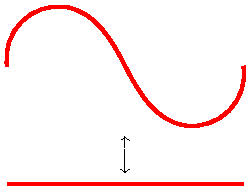
\includegraphics[width= 0.4\linewidth]{R0.pdf}\quad
		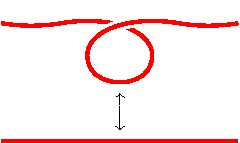
\includegraphics[width= 0.4\linewidth]{R1.pdf}
		\caption{\small\textit{\color{duongvaotoanhoc}R$0$: Phép đẳng luân phẳng.\hspace*{20pt}  RI: Phép xoắn.}}
		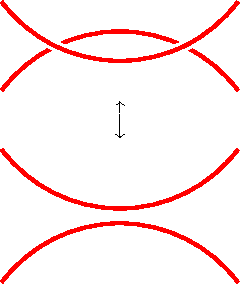
\includegraphics[width= 0.4\linewidth]{R2.pdf}\quad
		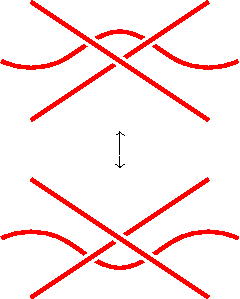
\includegraphics[width= 0.4\linewidth]{R3.pdf}
		\caption{\small\textit{\color{duongvaotoanhoc}RII: Phép đè.\hspace*{30pt} RIII: Phép trượt.}}
		\caption{\small\textit{\color{duongvaotoanhoc}Hình $14$: Các chuyển động Reidemeister.}}
		\vspace*{-10pt}
	\end{figure}
	Từ biểu đồ phẳng của nút, ta dùng các đại lượng không đổi qua các chuyển động Reidemeister, các {\bf\color{duongvaotoanhoc} bất biến nút}. Hai nút có bất biến khác nhau thì phải khác nhau. Một ví dụ như vậy là {\bf\color{duongvaotoanhoc} bất biến tô màu}. Ta nói một biểu đồ phẳng của nút là {\bf\color{duongvaotoanhoc} tô được bằng $\pmb{3}$ màu} nếu mỗi sợi (phần đường cong liên tục giữa hai giao điểm liên tiếp của nút) đều có thể tô được bằng một trong $3$ màu cho trước, sao cho
	\vskip 0.05cm
	$\bullet$ ít nhất hai màu phải được dùng;
	\vskip 0.05cm
	$\bullet$ tại mỗi giao điểm, sợi trên cùng $2$ sợi dưới hoặc là được tô cùng màu, hoặc là được tô $3$ màu khác nhau.
	\vskip 0.05cm
	Ví dụ, nút ba lá hiển nhiên tô được bằng $3$ màu, nút tầm thường hiển nhiên không tô được bằng $3$ màu. Nút số $8$ cũng không tô được bằng $3$ màu. Vậy ít nhất ta biết rằng nút $3$ lá không đẳng luân với nút tầm thường cũng như nút số $8$.
	\vskip 0.05cm
	Hiển nhiên là bất biến tô màu chỉ cho phép phân loại các nút thành $2$ lớp. Ta cần các loại bất biến khác. Ví dụ, xét nút ba lá trái và ảnh gương của nó là nút ba lá phải. Tất nhiên cả hai đều tô được bằng $3$ màu. Rất ngạc nhiên, hai nút này không đẳng luân! Hãy thử dùng các chuyển động Reidemeister để gỡ nút này thành nút kia và bạn sẽ sớm bị thuyết phục. Một bất biến cho phép phân biệt hai nút này là {\bf\color{duongvaotoanhoc} đa thức Alexander}. Đa thức này đến từ {\it lý thuyết Alexander--Fox}, và người ta phát hiện ra phiên bản số học của nó là {\it lý thuyết Iwasawa}. Sự song song của chúng cho phép ta dịch các kết quả từ một bên sang bên còn lại.
	\begin{figure}[H]
		\vspace*{-10pt}
		\centering
		\captionsetup{labelformat= empty, justification=centering}
		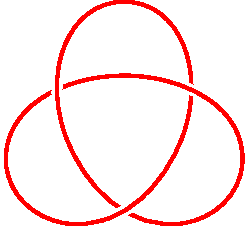
\includegraphics[width= 0.38\linewidth]{trefoil.pdf}\quad\quad
		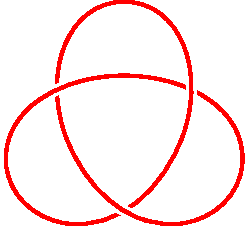
\includegraphics[width= 0.38\linewidth]{mirror trefoil.pdf}
		\caption{\small\textit{\color{duongvaotoanhoc}Hình $15$: Nút ba lá trái và nút ba lá phải.}}
		\vspace*{-10pt}
	\end{figure}
	Một kiểu bất biến khác cho liên kết là {\bf\color{duongvaotoanhoc} số liên kết}. Xét một liên kết được tạo bởi hai nút. Giữa hai nút $L$ và $K$, ta có thể định nghĩa {\bf\color{duongvaotoanhoc} số liên kết} qua biểu đồ phẳng của chúng như sau. Chẳng hạn, tô màu đỏ cho $L$ và màu xanh cho $K$, đồng thời định hướng cho chúng (mỗi nút có thể có $1$ trong $2$ hướng). Tại các điểm trên biểu đồ phẳng mà có một sợi của nút này nằm trên một sợi của nút kia hoặc ngược lại, ta đánh dấu $+$ hoặc $-$ theo quy tắc ở Hình $16$. Sau đó ta lấy số dấu cộng trừ đi số dấu trừ, và lấy kết quả chia đôi. Kết quả cuối cùng thu được được gọi là số liên kết $\text{lk}(L,K)$. Chẳng hạn, số liên kết của hai nút trong liên kết Hopf là $1$ hoặc $-1$, tùy theo cách định hướng hai nút.
	\begin{figure}[H]
		\vspace*{-5pt}
		\centering
		\captionsetup{labelformat= empty, justification=centering}
		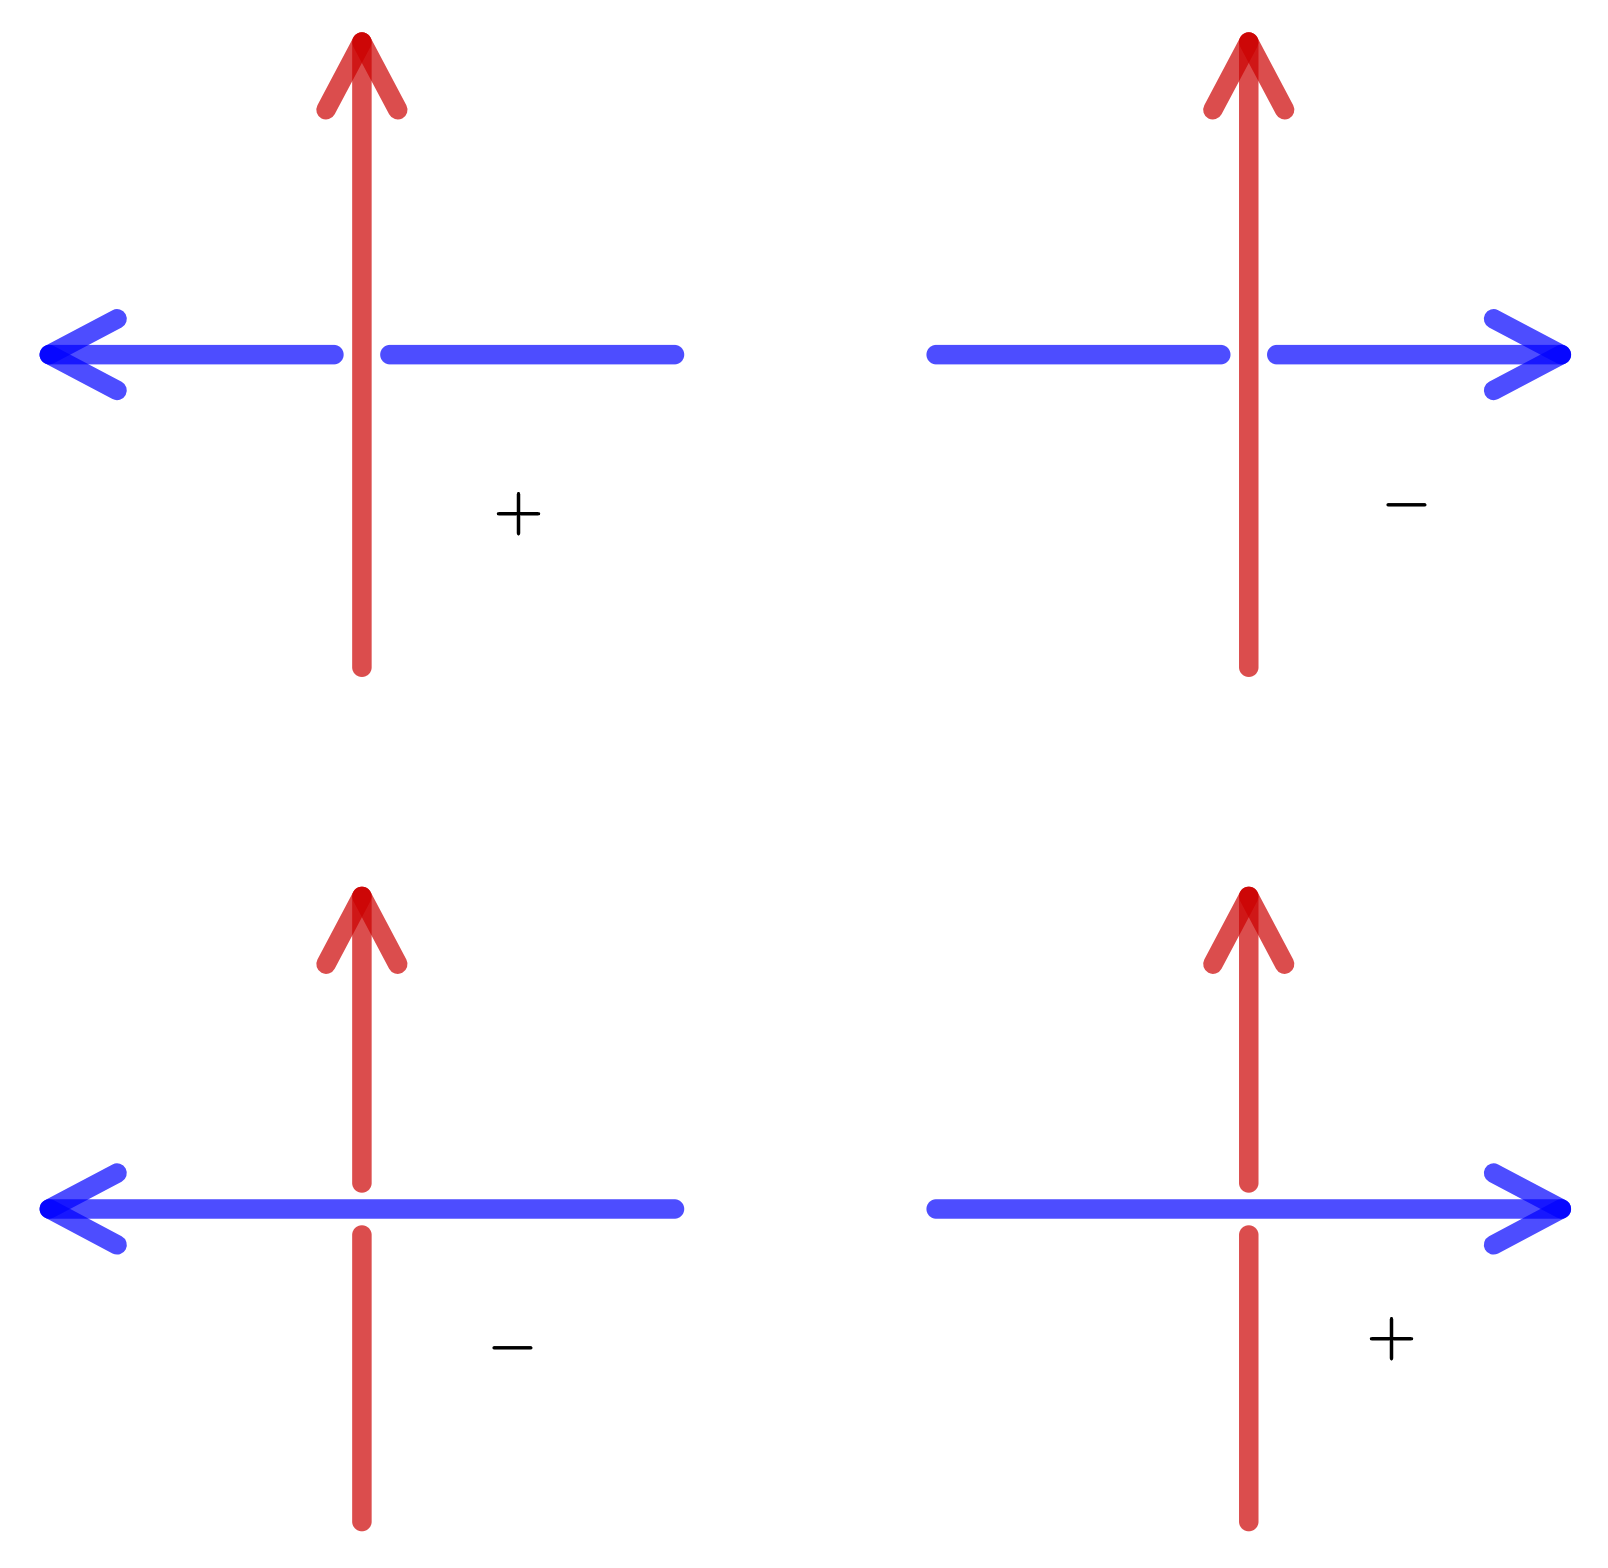
\includegraphics[width= 0.7\linewidth]{h16}
		\caption{\small\textit{\color{duongvaotoanhoc}Hình $16$: Quy tắc tính số liên kết.}}
		\vspace*{-10pt}
	\end{figure}
	Nhiều tính toán cho thấy rằng số liên kết thỏa mãn các tính chất tương tự như {\bf\color{duongvaotoanhoc} ký hiệu Legendre} $\left(\dfrac{p}{q}\right)$ giữa hai số nguyên tố $p, q$ trong lý thuyết thặng dư bậc hai. Ta có thể chứng minh rằng $\text{lk}(K,L) = \text{lk}(L,K)$. Tương ứng, ta có luật tương hỗ bậc hai, nói rằng 
	\begin{align*}
		\left(\dfrac{p}{q}\right) = (-1)^{\tfrac{(p-1)(q-1)}{4}}\left(\dfrac{q}{p}\right).
	\end{align*}
	Bài toán trung tâm của tôpô số học có lẽ là câu hỏi tự nhiên nhất: số nguyên tố nào ứng với nút nào? Đây vẫn là một câu hỏi mở. Nếu một ngày người ta xây dựng được một tương ứng $1-1$ tốt giữa chúng, theo nghĩa mỗi kết quả với số nguyên tố thì ta có kết quả với các nút tương ứng, một số lượng khổng lồ bài toán tôpô học sẽ được giải bằng các kết quả tương tự ở lý thuyết số, và ngược lại.
	\vskip 0.1cm
	Có thể nói, tôpô số học là một trong những ví dụ điển hình nhất về tư tưởng toán học thống nhất, rằng tất cả những đại số, giải tích, hình học, số học... đều chỉ là một.
\end{multicols}
\vspace*{-10pt}
{\color{duongvaotoanhoc}\rule{1\linewidth}{0.1pt}}
\vskip 0.2cm
\centerline{\LARGE{\textbf{\color{duongvaotoanhoc}LỜI GIẢI, ĐÁP ÁN}}}
\begin{multicols}{2}
	\textbf{\color{duongvaotoanhoc}Thám tử và $\pmb{50}$ tên cướp}
	\vskip 0.1cm
	Giả sử tất cả các tên cướp đều khai thật. Ta chọn một tên cướp bất kỳ, gọi tên là $A$. Tên này tham gia không quá $7$ vụ cướp, hơn nữa $49$ tên còn lại đều chỉ tham gia đúng duy nhất một vụ cướp chung với $A$. Theo nguyên lý Dirichlet, phải có một vụ cướp (đặt tên là $T$) mà có không ít hơn $7$ tên trong số $49$ tên còn lại tham gia. Cùng với $A$, sẽ có không ít hơn $8$ tên cướp tham gia vụ cướp $T$ này. Vì $50$ tên cướp không cùng tham gia một vụ, nên phải có một tên không tham gia vụ $T$. Ta gọi đó là tên cướp $B$. 
	\vskip 0.1cm
	Ta sẽ chỉ ra $B$ tham gia ít nhất $8$ vụ cướp. Thật vậy, theo kết luận điều tra $B$ có tham gia các vụ cướp cùng với mỗi tên trong số tất cả các tên tham gia vụ $T$, hơn nữa tất cả các vụ cướp đó là khác nhau.  Nếu không, sẽ có hai vụ cướp trùng nhau. Điều đó có nghĩa là có hai tên cướp (đặt tên là $X$ và $Y$) sao cho $B,X,Y$ cùng tham gia một vụ $S$ ($S$ khác với $T$); hơn nữa $X,Y$ cũng đã tham gia cả vụ cướp $T$. Suy ra $X,Y$ cùng tham gia cả $2$ vụ cướp khác nhau là $S$ và $T$. Điều này mâu thuẫn với kết luận điều tra.
	\vskip 0.1cm
	Mâu thuẫn trên chỉ ra phải có một tên cướp khai gian dối. Điều này có nghĩa ít nhất có một tên đã tham gia không ít hơn $8$ vụ cướp.
	\vskip 0.1cm
	\textbf{\color{duongvaotoanhoc}Góc cờ}
	\vskip 0.1cm
	Hình $4.$: $\pmb{1)}$ C$3.1$ X$4.2$\quad  $\pmb{2)}$ X$8.3$ P$5-6$\quad  $\pmb{3)}$ P$2-4$ M$7.6$\quad $\pmb{4)}$ P$4.4$ M$6.4$\quad $\pmb{5)}$ P$4/6$ (Đen mất xe, Đỏ chiếm ưu thế lớn).
	\vskip 0.1cm
	Hình $5.$: $\pmb{1)}$ X$1-4$ S$4.5$\quad  $\pmb{2)}$ X$4.4$ M$4.3$\quad $\pmb{3)}$ X$9.2$ M$3.2$\quad $\pmb{4)}$ X$9-8$ X$1-2$\quad $\pmb{5)}$ X$8.7$ M$3/2$\quad $\pmb{6)}$ C$7.1$ Ms$.1$\quad $\pmb{7)}$ X$4-7$ C$3.1$\quad  $\pmb{8)}$ X$7/3$ C$1.1$\quad $\pmb{9)}$ X$7-8$ (Đen chết Mã, Đỏ ưu thế lớn).	
	\vskip 0.1cm
	\hfill (\textit{Xem tiếp trang} ...)
%	\textbf{Đố vui}
%	\vskip 0.1cm
%	Cả Hổ và Sư Tử đều không thể tuyên bố ``Hôm qua tôi đã nói dối" vào ngày phải nói thật nếu ngày hôm trước cũng là một trong những ngày phải nói thật. Do đó, Hổ  không thể tuyên bố như vậy vào thứ Ba, thứ Tư  và thứ Năm; Sư Tử không thể tuyên bố như vậy vào thứ Bảy, Chủ nhật  và thứ Hai. 
%	Vì vậy, hôm mà các bạn nói như vậy chỉ có thể là thứ Sáu.
%	\vskip 0.1cm
\end{multicols}
	\newpage

	\setcounter{figure}{0}
	\thispagestyle{quantoannone}
\pagestyle{quantoan}
\everymath{\color{quantoan}}
\graphicspath{{../quantoan/pic/}}
\blfootnote{\color{quantoan}\color{quantoan}$^*$Lược dịch theo  https://mathshistory.st-andrews.ac.uk/Biographies/Arnold/}
\begingroup
\AddToShipoutPicture*{\put(0,616){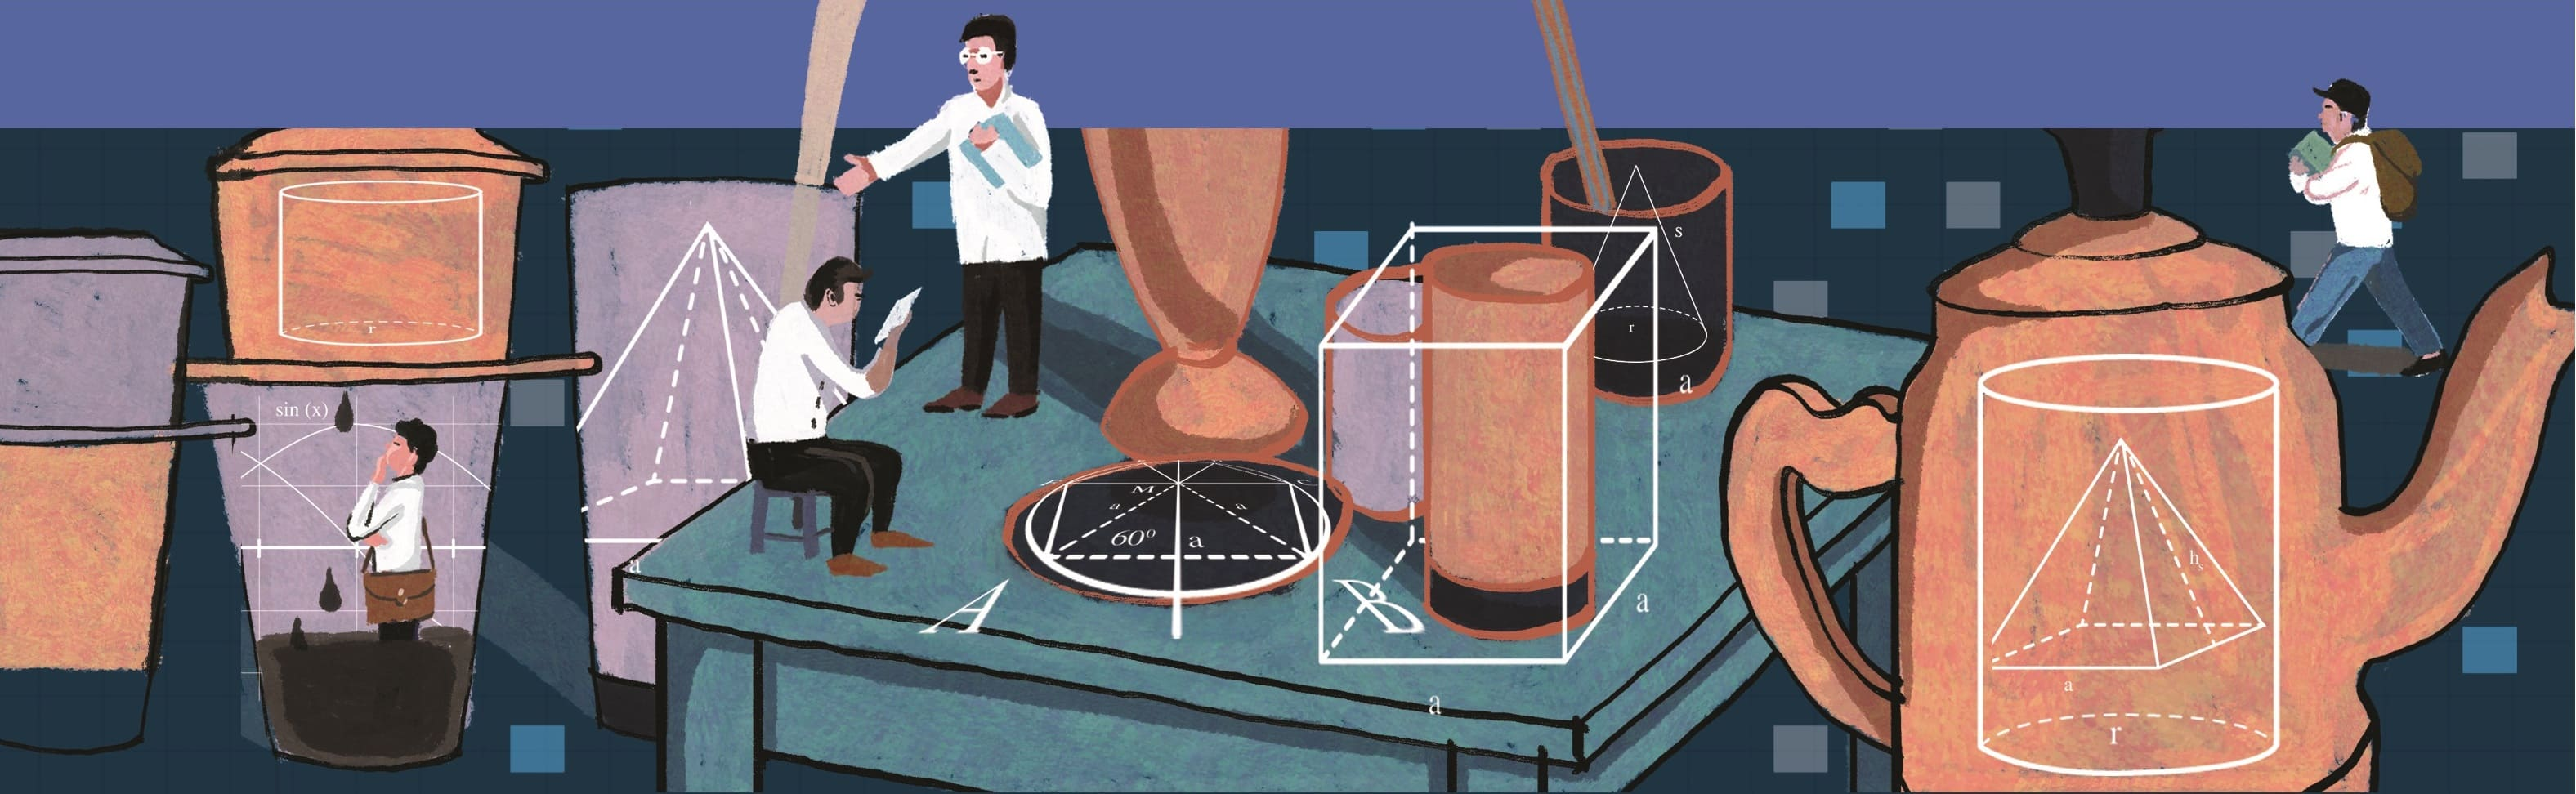
\includegraphics[width=19.3cm]{../bannerquantoan}}}
\AddToShipoutPicture*{\put(51,528){
\includegraphics[scale=0.9]{../tieude1.pdf}}}
\centering
\endgroup

\vspace*{180pt}

\begin{multicols}{2}	
	Vladimir Igorevich Arnold ($1937-2010$) là một nhà toán học sinh ra ở Ukraine, người đã giành được giải thưởng Wolf cho công trình nghiên cứu về hệ động lực học, phương trình vi phân và lý thuyết kỳ dị. Niềm đam mê toán học của Arnold được bắt đầu khi ông mới $5$ tuổi. Ông giải thích trong [$2$] rằng đây là một hệ quả của truyền thống toán học Nga.
	\begin{figure}[H]
		\vspace*{-5pt}
		\centering
		\captionsetup{labelformat= empty, justification=centering}
		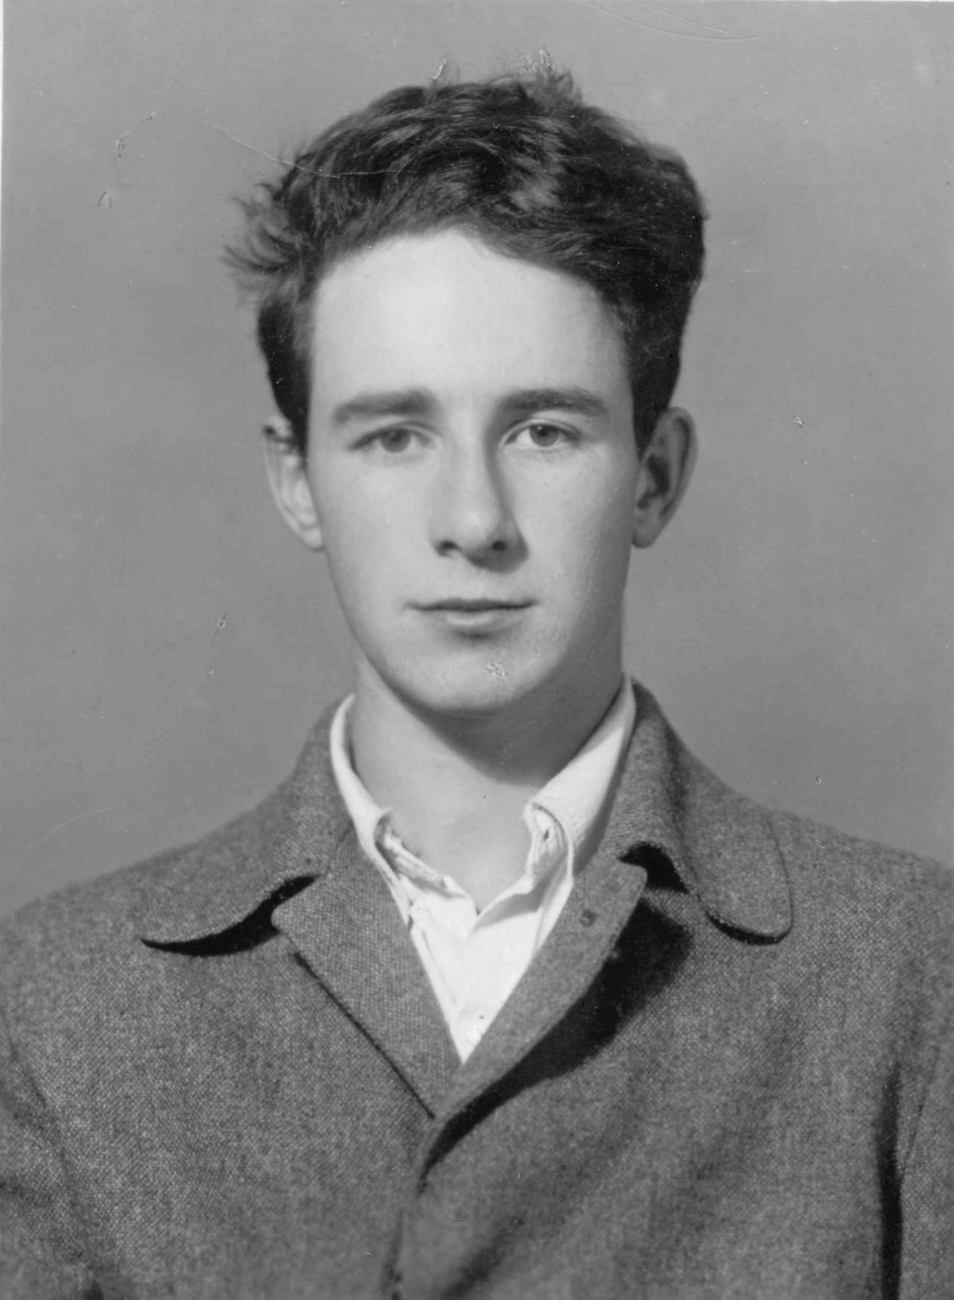
\includegraphics[width= 0.75\linewidth]{1}
		\caption{\small\textit{\color{quantoan}Vladimir Arnold vào năm $1957$.}}
		\vspace*{-10pt}
	\end{figure}
	\textit{Những  đứa trẻ khi còn rất nhỏ đã bắt đầu nghĩ về các bài toán (các bài toán cổ liên quan tới công việc buôn bán, trao đổi hàng hoá) ngay cả trước khi chúng có bất kỳ kiến thức nào về các con số. Trẻ em từ năm đến sáu tuổi rất thích các bài toán này và có thể giải được chúng, nhưng chính những bài toán đó lại có vẻ quá khó đối với những sinh viên tốt nghiệp đại học, những người đã bị làm hư bởi sự đào tạo toán học chính quy. ... Nhiều gia đình Nga có truyền thống đưa ra hàng trăm bài toán cho con cái của họ, và gia đình tôi cũng không ngoại lệ.}
	\vskip 0.1cm
	Khi mười hai tuổi, Arnold được thầy cô giáo  giao những bài toán khó. Ông trích dẫn một bài toán  như vậy trong [$2$]:
	\vskip 0.1cm
	\textit{Hai bà già bắt đầu đi từ lúc mặt trời mọc và mỗi người đi với vận tốc không đổi. Một người đi từ $A$ đến $B$ và người kia từ $B$ đến $A$. Họ gặp nhau vào giữa trưa và đi tiếp tục không nghỉ, lần lượt đến $B$ lúc $4$ giờ chiều,  và tới $A$ lúc $9$ giờ tối. Hỏi mặt trời mọc lúc mấy giờ vào ngày hôm đó?}
	\vskip 0.1cm
	Arnold thuật lại: 
	\vskip 0.1cm
	\textit{Tôi đã dành cả ngày để suy nghĩ về bài toán cũ kỹ đó, và lời giải ...  bỗng đến như một sự khám phá. Cảm giác khám phá mà tôi có lúc đó giống hệt như trong tất cả các bài toán nghiêm túc hơn nhiều về sau này ...}
	\vskip 0.1cm
	Là một nhà toán học nổi tiếng cả trong lĩnh vực nghiên cứu và giảng dạy, tuy nhiên Arnold luôn nhớ lại những năm tháng học đại học của mình với sự tôn trọng và đánh giá cao dành cho từng giáo sư được theo học và các bạn bè đồng môn. Ông kể lại trong [$2$]
	\vskip 0.1cm
	\textit{Sự quy tụ các ngôi sao toán học vĩ đại  trong cùng một khoa khi tôi theo học tại Khoa Toán -- Cơ là thực sự đặc biệt, và tôi chưa từng thấy điều gì giống như vậy ở bất kỳ nơi nào khác. Kolmogorov, Gelfand, Petrovsky, Pontryagin, P. Novikov, Markov, Gelfond, Lusternik, Khinchin và P. S. Aleksandrov lúc đó giảng dạy các sinh viên như Manin, Sinai, Sergei Novikov, V. M. Alexeev, Anosov, A. A. Kirillov và tôi. Tất cả những nhà toán học này đều rất khác nhau! Hầu như không thể hiểu được các bài giảng của Kolmogorov, nhưng chúng chứa đầy những ý tưởng và thực sự bổ ích! ... Pontryagin khi đó đã trở nên rất yếu lúc tôi là sinh viên của Khoa Toán Cơ, nhưng có lẽ ông ấy là giảng viên giỏi nhất của Khoa.}
	\begin{figure}[H]
		\vspace*{-5pt}
		\centering
		\captionsetup{labelformat= empty, justification=centering}
		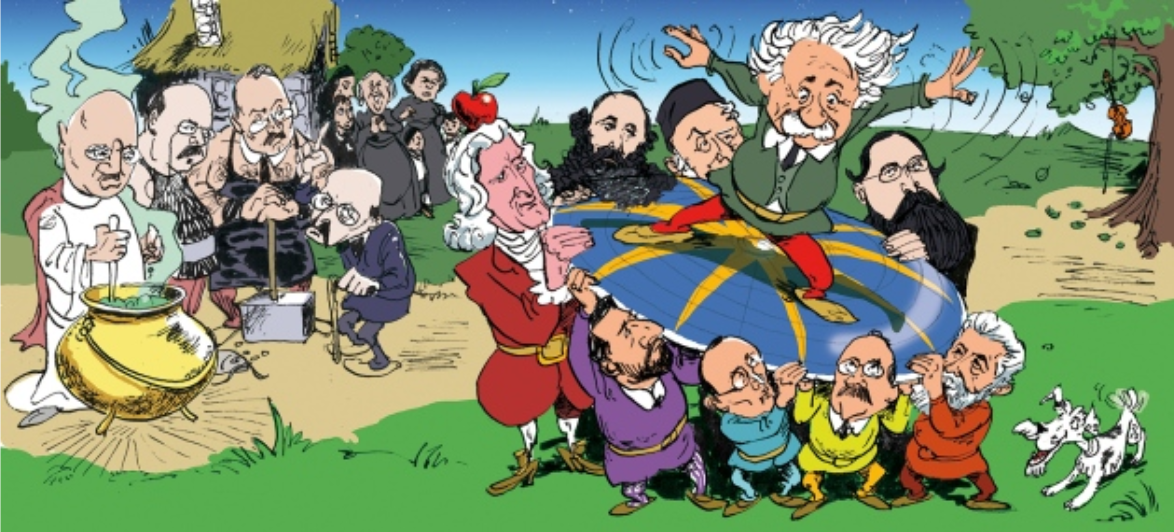
\includegraphics[width= 1\linewidth]{2}
		\caption{\small\textit{\color{quantoan}Thầy giáo Arnold cùng các học sinh Trường nội trú Toán Mátx--cơ--va vào những năm $1960$.}}
		\vspace*{-10pt}
	\end{figure}
	Năm $1965$, Arnold trở thành Giáo sư tại Khoa Toán -- Cơ tại Đại học Quốc gia Mát--xcơ--va, vị trí mà ông giữ cho đến năm $1986$ khi ông đảm nhận vị trí Nghiên cứu viên chính tại Viện Toán học Steklov ở Mát--xcơ--va. Ngoài các chức vụ ở Nga, năm $1993$, ông còn được bổ nhiệm làm Giáo sư tại Đại học Paris--Dauphine ở Pháp. Ông giữ chức vụ này cho đến năm $2005$.
	\vskip 0.1cm
	Khi nhận xét về cuốn sách Các bài toán của Arnold [$1$], Sergi Tabachnikov đã viết như sau trong [$4$] về các seminar của ông.
	\vskip 0.1cm
	\textit{Đời sống toán học ở Liên Xô từ cuối những năm $1950$, đặc biệt là ở Mát--xcơ--va, nổi tiếng với các seminar, như các seminar của Gelfand, Sinai, Kirillov, Manin, Novikov. Hầu hết các seminar này họp hàng tuần trong hai giờ, vào cuối buổi chiều. Đối với một số nhà toán học lỗi lạc, những seminar này là một cơ hội để thu hút và nuôi dưỡng những tài năng toán học mới chớm nở. Một trong những seminar nổi tiếng  là seminar của Arnold, tồn tại hơn $30$ năm. Mỗi học kỳ, buổi khai mạc của seminar luôn được dành cho các vấn đề mở. Arnold luôn trao đổi về hàng chục bài toán nghiên cứu với những bình luận chi tiết. Nhiều bài toán trong số này sau đó đã được giải quyết (hoặc giải quyết được một phần) bởi những người tham gia seminar. Theo Arnold, chu kỳ bán phân  rã của một bài toán là bảy năm. Nhiều người tham gia seminar cũng là nghiên cứu sinh của Arnold. Triết lý của ông luôn là: một sinh viên nên học được từ giáo viên của mình rằng một bài toán nào đó hiện đang là vấn đề mở; sự lựa chọn của một vấn đề nghiên cứu cụ thể sau đó là tùy thuộc vào sinh viên.}
	\begin{figure}[H]
		\vspace*{-5pt}
		\centering
		\captionsetup{labelformat= empty, justification=centering}
		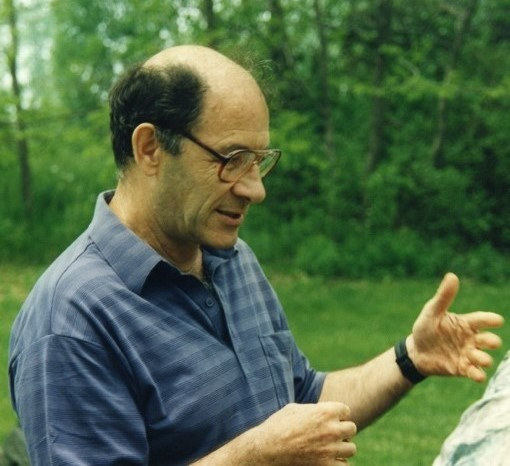
\includegraphics[width= 1\linewidth]{4}
		\caption{\small\textit{\color{quantoan}Vladimir Arnold vào năm $1997$.}}
		\vspace*{-10pt}
	\end{figure}
	Một cái nhìn tổng quan tuyệt vời về những đóng góp của Arnold đã được đưa ra trong phần trích dẫn về Giải thưởng Wolf được trao cho ông vào năm $2001$.
	\vskip 0.1cm
	\textit{Vladimir I. Arnold đã có những đóng góp đáng kể cho một số lượng đáng kinh ngạc các ngành toán học khác nhau. Nhiều công trình nghiên cứu, sách vở, bài giảng cộng với sự uyên bác và tâm huyết của ông đã có ảnh hưởng sâu sắc đến cả một thế hệ các nhà toán học. Luận án Tiến sĩ của Arnold có chứa một lời giải cho bài toán thứ $13$ của Hilbert. Công trình của ông về động lực học Hamilton, bao gồm việc đồng sáng tạo ra lý thuyết KAM (Kolmogorov--Arnold--Moser) và khám phá ra ``sự khuếch tán của Arnold", đã khiến ông nổi tiếng thế giới ngay từ khi còn nhỏ. Những đóng góp của Arnold cho lý thuyết kỳ dị bổ sung cho lý thuyết thảm họa của Thom và đã làm biến đổi lĩnh vực này. Arnold cũng đã có vô số đóng góp cơ bản cho lý thuyết phương trình vi phân, hình học symplectic, hình học đại số thực, phép tính biến phân, thủy động học và từ--thủy động học.  Ông thường phát hiện ra mối liên hệ giữa các vấn đề trong các lĩnh vực khác nhau.}
	\begin{figure}[H]
		\vspace*{-5pt}
		\centering
		\captionsetup{labelformat= empty, justification=centering}
		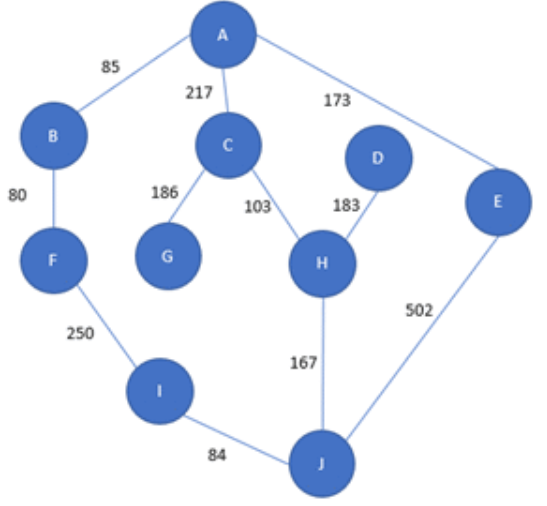
\includegraphics[width= 1\linewidth]{3}
		\caption{\small\textit{\color{quantoan}Giáo sư Arnold trong một buổi giảng bài.}}
		\vspace*{-10pt}
	\end{figure}
	Khi Arnold tròn $65$ tuổi vào năm $2002$, Tạp chí Toán học Mát--xcơ--va (Mát--xcơ--va Mathematical Journal) đã dành hai số báo để chào mừng sự kiện này với phần giới thiệu như sau: 
	\vskip 0.1cm
	\textit{...Bộ mặt của toán học hiện đại sẽ không thể nhận ra được nếu không có những công trình của ông trong các lĩnh vực như hệ động lực, cơ học cổ điển và cơ học thiên thể, lý thuyết  kỳ dị, tô pô, hình học đại số thực và phức, hình học symplectic và hình học tiếp xúc, thủy động học, phép tính biến phân, hình học vi phân, lý thuyết thế vị, vật lý toán học, lý thuyết chồng chất, v.v...
	\vskip 0.1cm
	Arnold là một giáo viên hiếm có, trường lớp của ông luôn nổi tiếng và đông đảo người theo, ông có năng khiếu đặc biệt trong việc tìm ra những vấn đề mới và  hấp dẫn để thu hút sự quan tâm và lôi cuốn các nhà nghiên cứu trẻ. Ông là một giảng viên phi thường ở tất cả các cấp giáo dục toán học và nghiên cứu. Những lý thuyết hiện đại khó hiểu trở nên khá rõ ràng và đơn giản trong phần trình bày của ông. Người ta khó có thể hình dung nền giáo dục toán học hiện đại nếu không có những cuốn sách giáo khoa xuất sắc của ông. Trường phái toán học Mát--xcơ--va phải mang ơn rất nhiều những seminar của ông.
	\vskip 0.1cm
	Xuất thân từ một gia đình nhiều thế hệ làm khoa học, ông tập hợp được cách tiếp cận khoa học của họ và mối quan tâm sâu sắc đến mọi mặt của cuộc sống, kiến thức của ông vô cùng rộng lớn và sự tò mò của Arnold đối với mọi thứ xung quanh thật tuyệt vời.}
	\vskip 0.1cm
	Arnold đã được trao Giải thưởng Nhà nước của Liên bang Nga ($2007$), và trong năm tiếp theo, ông đã nhận được Giải thưởng Shaw danh giá về khoa học toán học.
	\vskip 0.1cm
	Arnold đã có lần trả lời trong một bài phỏng vấn [$3$]: ``\textit{Người học không phải là chiếc túi phải lấp đầy, mà là ngọn đuốc cần được thắp sáng}".
	\vskip 0.1cm
	\textbf{\color{quantoan}Tài liệu tham khảo}
	\vskip 0.1cm
	[$1$] Vladimir I. Arnold (ed.). Arnold's Problems. \textit{Springer--Verlag, Berlin--Heidelberg--New York $\&$ PHASIS}, Mát--xcơ--va, $2005$, XV.
	\vskip 0.1cm
	[$2$]	S. H. Lui, An interview with Vladimir Arnold, \textit{Notices Amer. Math. Soc.} $44$ ($4$) ($1997$), $432-438$.
	\vskip 0.1cm
	[$3$]	S. Tabachnikov. Interview with V. I. Arnold. (\textit{in Russian}) \textit{Kvant} $1990$, No $7$, $2-7$, $15$.
	\vskip 0.1cm
	[$4$]	S. Tabachnikov. Arnold's Problems. \textit{The Mathematical Intelligencer.} $2007$
\end{multicols}
\newpage
\begingroup
\AddToShipoutPicture*{\put(132,678){
\includegraphics[scale=1]{../tieude2.pdf}}}
\centering
\endgroup
\blfootnote{$^1$\color{quantoan}Viện Vật lý.}
\vspace*{30pt}

\begin{multicols}{2}
	Richard Feynman ($1918-1988$, Mỹ) nổi tiếng là người trung thực không khoan nhượng và đam mê đến tận cùng. Về tính trung thực, người ta hay nhắc đến vụ ông trình diễn trực tiếp trên TV một ``thí nghiệm nhỏ", bỏ vòng cao su vào cốc nước đá, minh chứng rằng cao su mất tính đàn hồi ở nhiệt độ thấp, qua đó chỉ ra nguyên nhân dẫn đến thảm họa tàu vũ trụ con thoi ``Challenger", vạch trần chiến dịch tung hỏa mù của NASA về nguyên nhân của thảm họa này. Để công bố với người dân Mỹ sự thật ấy, Feynman đã phải vượt qua sức ép khủng khiếp từ các cơ quan công quyền Mỹ, trong đó có CIA và NASA. 
	\begin{figure}[H]
		\vspace*{-5pt}
		\centering
		\captionsetup{labelformat= empty, justification=centering}
		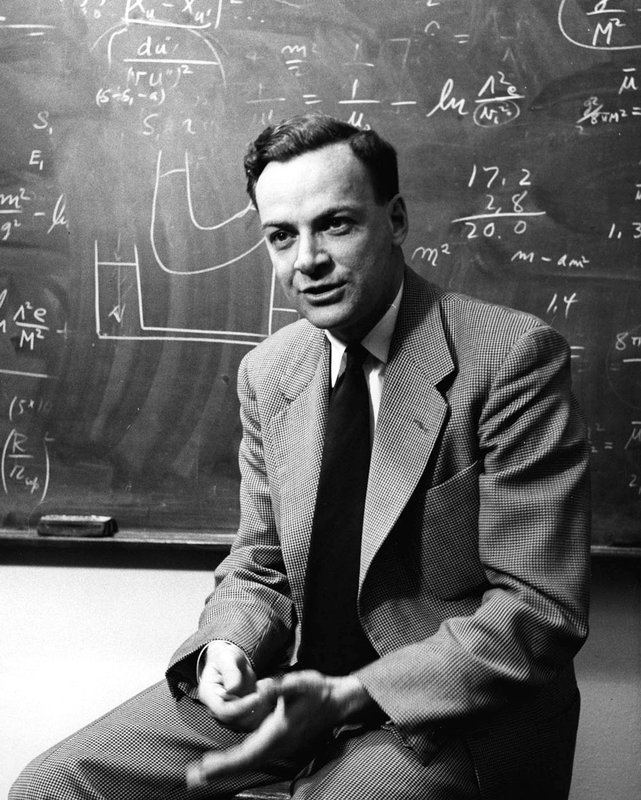
\includegraphics[width= 1\linewidth]{1a}
		\caption{\small\textit{\color{quantoan}Richard Feynman (ảnh từ bộ sưu tập của Học viện Công nghệ California, CalTech).}}
		\vspace*{-10pt}
	\end{figure}
	Lắm đam mê. Đam mê Vật lý, Feynman nhận giải Nobel Vật lý năm $1965$. Đam mê chơi trống, vở ba--lê do ông đệm trống nhận giải nhất trong cuộc thi ba--lê toàn nước Mỹ và giải nhì trong cuộc thi quốc tế tại Paris. Đam mê vẽ, ông đã có triển lãm tranh riêng. Không rõ, ông biết những ngôn ngữ nào, chỉ biết, thăm Brazil ông dạy bằng tiếng Bồ, thăm Nhật ông giao du bằng tiếng Nhật. Rồi có lần bạn bè định ``cho ông một vố", họ nhờ một cô Hoa kiều đón tiếp ông bằng tiếng Trung, Feynman đáp lại và cô ấy kêu Trời, vì ông nói tiếng Quảng Đông, còn cô chỉ nói tiếng Băc Kinh. Rất nhiều ``Đam mê" kiểu như vậy được kể trong cuốn ``Feynman, chuyện như thật đùa" (NXB Trẻ) và hầu như tất cả đều có kết cục mỹ mãn, kiểu như giải Nobel. Có thể Bạn nghĩ, chắc ông này ``con nhà nòi", học ``trường quốc tế" từ nhỏ! Xin thưa, bố của Feynman là người bán rong quần áo, còn mẹ thì nội trợ. 
	\begin{figure}[H]
		\vspace*{-5pt}
		\centering
		\captionsetup{labelformat= empty, justification=centering}
		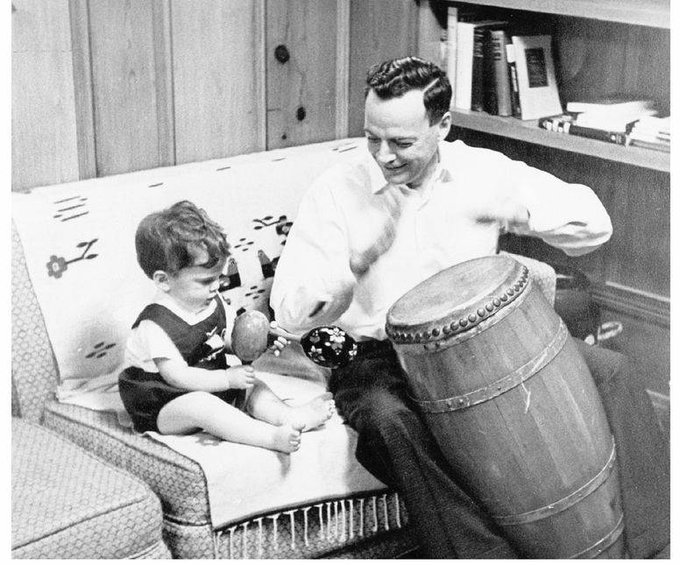
\includegraphics[width= 1\linewidth]{2a}
		\caption{\small\textit{\color{quantoan}Feynman chơi trống bên con trai (ảnh từ Internet).}}
		\vspace*{-10pt}
	\end{figure}
	Ông chơi trống (bongo) cực giỏi, nhưng chưa bao giờ học nhạc lý. Ông vốn vẽ rất kém, tự nhận chẳng thể vẽ nổi cái gì ngoại trừ cái kim tự tháp chỉ gồm mấy đường thẳng. Để học vẽ, Feynman ``đổi công" với một họa sĩ: ông dạy Vật lý cho họa sĩ còn họa sĩ dạy vẽ cho ông. Hãy tưởng tượng một giáo sư nổi tiếng thế giới ngồi trong lớp vẽ cùng các cháu $8-9$ tuổi học cách gọt bút chì. Đam mê như thế chỉ có ở Feynman. Và, với ông Đam mê chính là nguồn cội của Thành công, chứ chẳng phải ``con nhà nòi" hay ``Trường quốc tế" nào cả. Tiền bạc và chứng chỉ đầy người, mà không đam mê gì, thì làm sao có thành quả! 
	\begin{figure}[H]
		\vspace*{-5pt}
		\centering
		\captionsetup{labelformat= empty, justification=centering}
		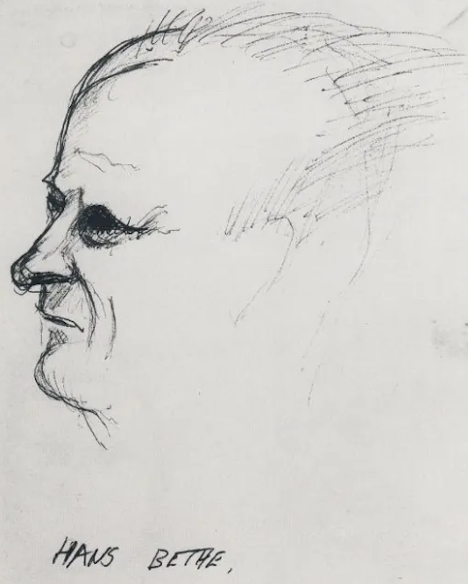
\includegraphics[width= 1\linewidth]{3a}
		\caption{\small\textit{\color{quantoan}Feyman vẽ Hans Bethe (giải Nobel Vật lý $1967$).}}
		\vspace*{-10pt}
	\end{figure}
	Duy có đam mê cuối cùng, Feynman đã không kịp nhìn thấy những gì mình muốn, trước khi về cõi vĩnh hằng. Đó là ``Cuộc phiêu lưu cuối cùng của Feynman"\footnote[2]{\color{quantoan}Xem thêm: Cuộc phiêu lưu cuối cùng của Feynman, in lần $2$, NXB Trẻ $2023$.}. Cuộc phiêu lưu khởi đầu bằng một con tem có xuất xứ từ một nơi gọi là Tannu Tuva, mà Feynman có được từ khi còn nhỏ. Cái tên ``Tuva" xa lạ nằm yên trong đầu Feynman, cho đến một ngày hè $1977$ nó trở thành mục tiêu cho ``cuộc phiêu lưu" kéo dài hơn $10$ năm cuối của cuộc đời Ông. Tôi cược là nhiều bạn chưa biết Tuva là địa danh nào và ở đâu. Để đỡ tra cứu, xin bật mí ngay: đó là tên một quốc gia nhỏ nằm giáp Tây Bắc của Mông Cổ, vốn độc lập, nhưng đã sáp nhập vào Liên Xô cũ (và Nga ngày nay). Thủ đô của Tuva là Kyzyl. Tuva có gì đặc biệt mà khiến Feynman mê mệt đến vậy?
	\vskip 0.1cm
	Bạn có biết, đâu là trọng tâm của lục địa châu Á (lục địa thôi chứ không tính các đảo)? Lấy tấm bìa cứng phẳng, vẽ lên đó bản đồ Á lục, cắt theo đường biên để được miếng bìa hình lục địa châu Á. Dùng một chiếc bút đầu nhọn chống phía dưới tấm bìa, di di đầu bút, để tìm vị trí mà tấm bìa nằm cân bằng trên chiếc bút thẳng đứng. Vị trí đó rơi vào Kyzyl, trọng tâm của Á lục. Tất nhiên, các nhà khoa học xác định điểm này bằng các phương pháp chính xác hơn, và ngày nay ở Kyzyl có tấm bia lớn khẳng định vị trí đặc biệt của mình. Nhưng, chỉ chừng ấy, thì không đủ để Feynman mất tới cả chục năm tìm cách tới thăm Tuva.
	\begin{figure}[H]
		\vspace*{-5pt}
		\centering
		\captionsetup{labelformat= empty, justification=centering}
		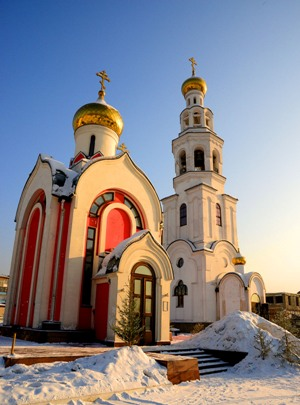
\includegraphics[width= 1\linewidth]{4a}
		\caption{\small\textit{\color{quantoan}Nhà thờ Phục sinh ở Kyzyl, Tuva (ảnh từ Internet).}}
		\vspace*{-10pt}
	\end{figure}
	Cái chính là ở quốc gia tí xíu bao bọc bởi những dãy núi cao ấy, thời gian gần như ngừng trôi: tất cả vẫn nguyên sơ như $500$ hay $1000$ năm trước. Thảo nguyên hoang dại. Những đàn tuần lộc hay bò Tây tạng cũng dường như hoang dại. Cuộc sống du mục không thể tự nhiên hơn. Một nền văn hóa xa xưa và kỳ thú với kiểu hát hai giọng chỉ có ở Tuva, với thứ văn tự không thể tìm thấy trong bất cứ tự điển nào, với các tập tục rất lạ điều hành bởi các tù trưởng uy nghi và bí ẩn vv\ldots Tiếc là, ít người biết Tuva, chứ không, người ta đã gọi quốc gia này là ``Thảo nguyên Xanh" cuối cùng của hành tinh Trái Đất (như Công--gô là Hành tinh Xanh cuối cùng!). Đam mê Tuva, Feynman tìm đọc mọi tài liệu về Tuva, tìm hiểu văn tự Tuva, học cách hát của dân du mục Tuva, ăn mặc và trang trí như Tù trưởng Tuva\ldots Và, nhất là, ông tìm mọi cách để có thể đến thăm Tuva.
	\vskip 0.1cm
	Đó là thời ``Chiến tranh lạnh", lại nghe nói, gần Tuva có một cơ sở nghiên cứu bom nguyên tử, nên nơi đây là ``vùng cấm" với khách du lịch, nhất là khách nước ngoài. Thực ra, Viện Hàn lâm Khoa học Liên xô sẵn sàng mời Feynman sang Matx--cơ--va đọc bài giảng rồi đi ``tham quan Kyzyl" theo kiểu mặc com--lê ở hotel có người bảo vệ vv\ldots Nhưng, Feynman không thích như vậy, mà muốn tự mình mang ba lô đến thảo nguyên, ngủ lều, uống sữa tuần lộc và hát hai giọng cùng dân bản xứ. Ấy thế cho nên Ông mất cả chục năm tìm kiếm một giấy mời như mình muốn. Và, đầu tháng Ba $1988$, một giấy mời như thế đã gửi đến địa chỉ của Feynman, chỉ tiếc là hai tuần trước đó, vào ngày $15$ tháng Hai, Ông đã ra đi mãi mãi, nên chỉ có thể trải nghiệm ``Cuộc phiêu lưu cuối cùng" của mình trong tâm trí và trái tim của những người ở lại. Không rõ, ở Thế giới bên kia Feynman đang đam mê cái gì?
\end{multicols}
	\newpage

	\setcounter{figure}{0}
	\thispagestyle{toancuabinone}
\pagestyle{toancuabi}
\everymath{\color{toancuabi}}
\blfootnote{$^1$\color{toancuabi}Trường Liên cấp Hội nhập Quốc tế iSchool Quảng Trị.}
\graphicspath{{../toancuabi/pic2/}}
\begingroup
\AddToShipoutPicture*{\put(0,616){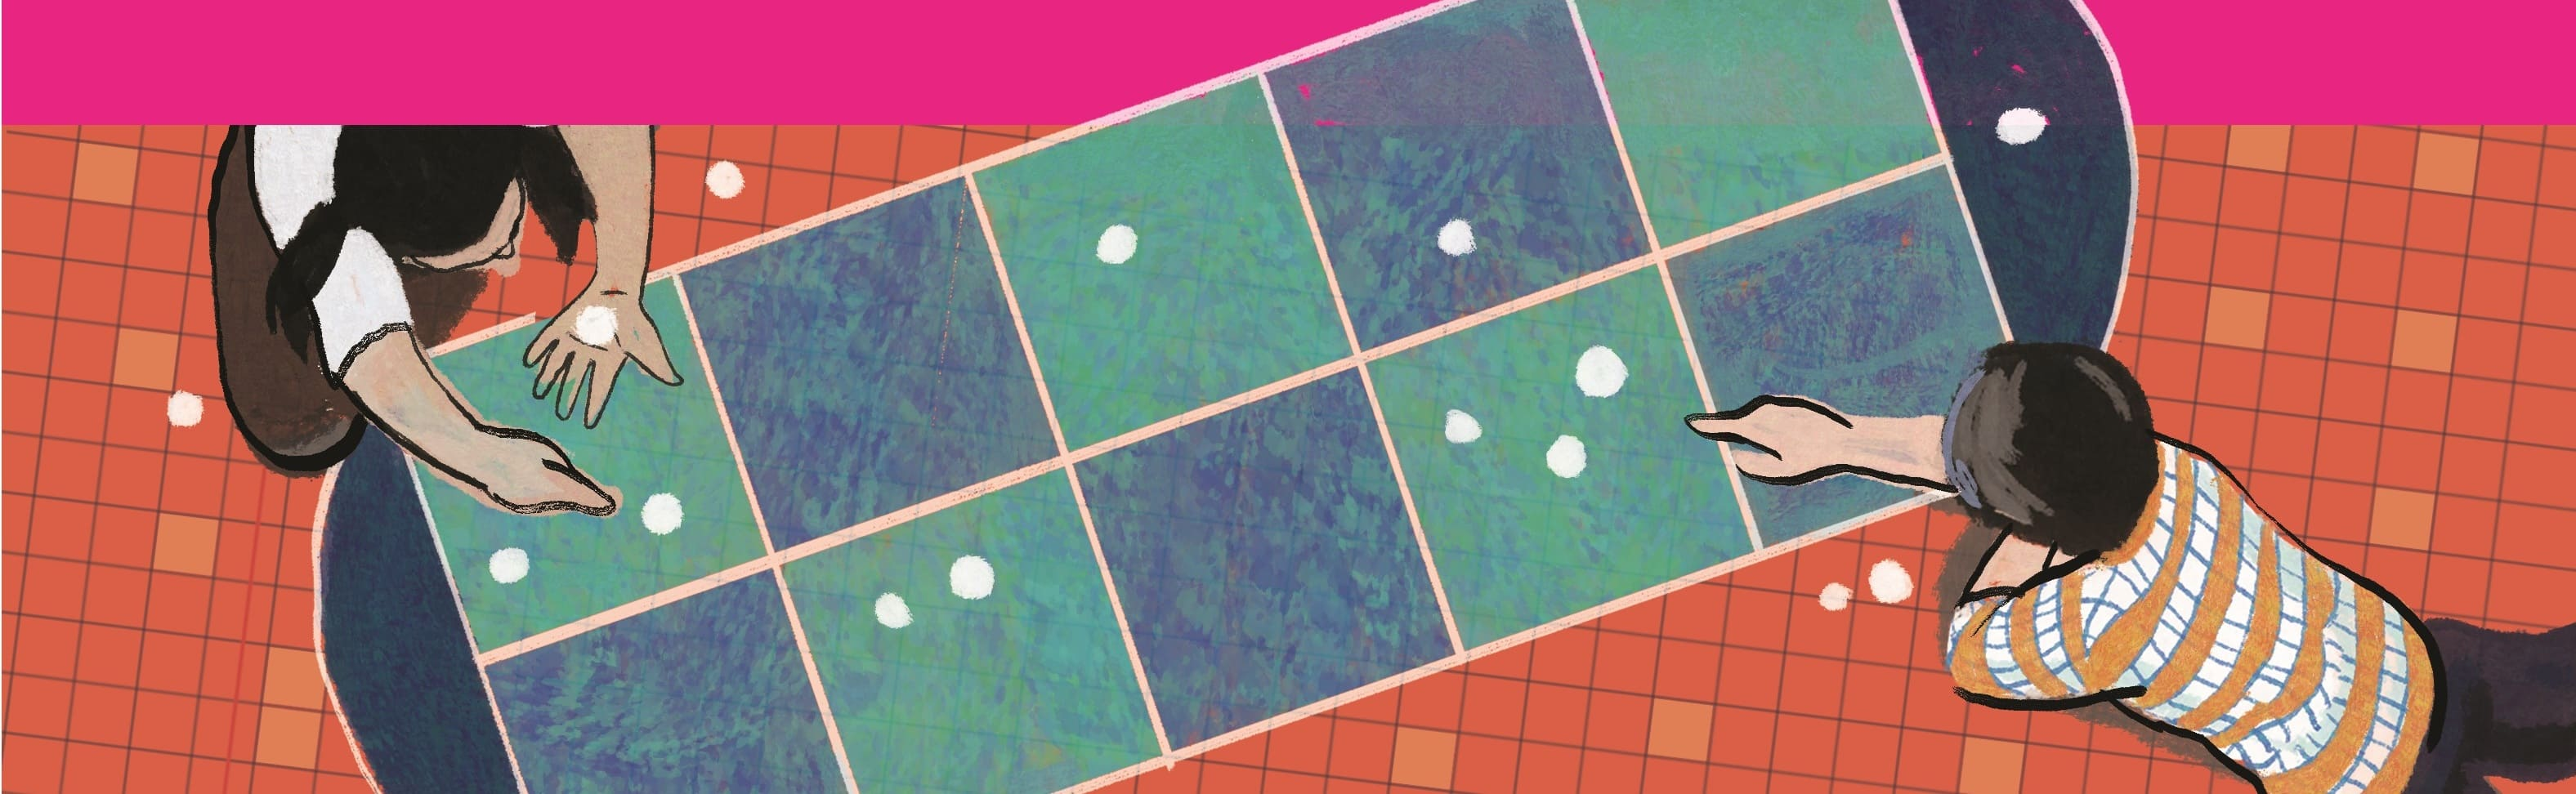
\includegraphics[width=19.3cm]{../bannertoancuabi}}}  
\AddToShipoutPicture*{\put(110,525){
\includegraphics[scale=1]{../tieude10.pdf}}}  
\centering
\endgroup
\vspace*{185pt} 

\begin{multicols}{2}
	Chuồn chuồn tre là sản phẩm độc đáo được các nghệ nhân làng Thạch Xá tạo nên, là món đồ chơi tuổi thơ rất đỗi thân thuộc đối với mỗi người dân trong làng. Lịch sử làng chuồn chuồn tre Thạch Xá với nhiều năm trong nghề đã biến mảnh đất này thành một trong những làng nghề nổi tiếng ở Hà Nội được nhiều du khách biết đến.
	\begin{center}
		\textit{Chuồn chuồn có cánh thì bay\\
			Có thằng cu Tí thò tay bắt chuồn}
	\end{center}
	\hfill \textit{(Đồng dao, thơ ca dân gian)}
	\begin{figure}[H]
		\vspace*{-5pt}
		\centering
		\captionsetup{labelformat= empty, justification=centering}
		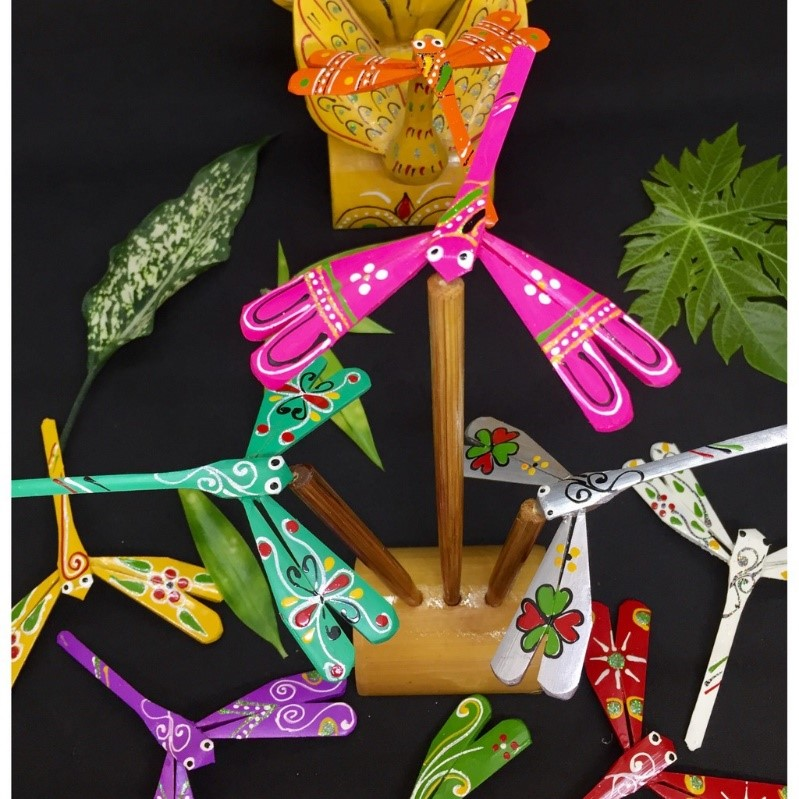
\includegraphics[width= 0.85\linewidth]{10}
		\caption{\small\textit{\color{toancuabi}Ảnh : Internet.}}
		\vspace*{-10pt}
	\end{figure}
	Ngày hôm nay chúng ta sẽ cùng nhau thử sức làm chuồn chuồn tre nhé! Để đơn giản hơn thì chúng ta sẽ thay thế vật liệu để làm chuồn chuồn tre là từ những cây tre thành que kem hoặc giấy.
	\vskip 0.1cm
	\textbf{\color{toancuabi}Cách $\pmb{1}$: Chuồn chuồn que kem thăng bằng}
	\vskip 0.1cm
	\textit{Chuẩn bị nguyên liệu}: 
	\vskip 0.05cm
	-- Các que kem.
	\vskip 0.05cm
	-- Keo, súng bắn keo.
	\vskip 0.05cm
	-- Đũa dùng một lần.
	\vskip 0.05cm
	-- Thước thẳng.
	\vskip 0.05cm
	-- Dao rọc giấy.
	\vskip 0.05cm
	-- Bút chì.
	\vskip 0.05cm
	\textit{Cách làm chuồn chuồn que kem thăng bằng}:
	\vskip 0.1cm
	\textit{Bước} $1$: Sử dụng súng bắn keo dính hai que kem dài $4$ cm lại với nhau.
	\begin{figure}[H]
		\vspace*{-5pt}
		\centering
		\captionsetup{labelformat= empty, justification=centering}
		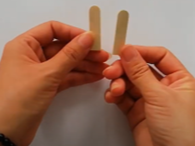
\includegraphics[height=0.37\linewidth]{11}
		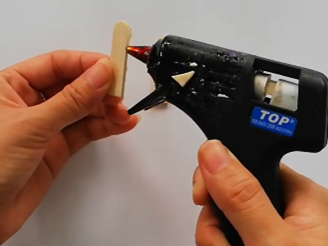
\includegraphics[height=0.37\linewidth]{12}
		
		\vspace*{1pt}
		\includegraphics[width=1\linewidth]{13}
%		\vspace*{-5pt}
	\end{figure}
	\textit{Bước} $2$: Sử dụng đầu que kem và bút chì để tạo hình phần đầu cho con chuồn chuồn.
	\begin{figure}[H]
		\vspace*{-5pt}
		\centering
		\captionsetup{labelformat= empty, justification=centering}
		\includegraphics[width=0.7\linewidth]{14}
		
		\vspace*{1pt}
		\includegraphics[width=0.7\linewidth]{15}
		
		\vspace*{1pt}
		\includegraphics[width=0.7\linewidth]{16}
		
		\vspace*{1pt}
		\hspace*{1pt}\includegraphics[width=0.7\linewidth]{17}
		\vspace*{-5pt}
	\end{figure}
	\textit{Bước} $3$: Sử dụng dao rọc giấy cắt đi phần khuyết.
	\begin{figure}[H]
		\vspace*{-5pt}
		\centering
		\captionsetup{labelformat= empty, justification=centering}
		\includegraphics[width=0.7\linewidth]{18}
		
		\vspace*{1pt}
		\hspace*{1pt}\includegraphics[width=0.7\linewidth]{19}
		\vspace*{-10pt}
	\end{figure}
	\textit{Bước} $4$: Lấy que kem nguyên vẹn rồi cắt chéo đi một nửa (như hình minh họa), sau đó dùng súng bắn keo dán vào que kem dài $10$~cm để làm cánh chuồn chuồn. (Lưu ý là chuồn chuồn có cánh dài, cánh ngắn).
	\begin{figure}[H]
		\vspace*{5pt}
		\centering
		\captionsetup{labelformat= empty, justification=centering}
		\includegraphics[height=0.35\linewidth]{50}
		\includegraphics[height=0.35\linewidth]{51}
		
		\vspace*{1pt}
		\includegraphics[width=0.7\linewidth]{52}
		
		\vspace*{1pt}
		\includegraphics[width=0.7\linewidth]{53}
		
		\vspace*{1pt}
		\includegraphics[width=0.7\linewidth]{54}
		\vspace*{-10pt}
	\end{figure}
	\textit{Bước} $5$: Sử dụng súng bắn keo để dán que kem dài $10$ cm vào phần đầu của con chuồn chuồn.
	\begin{figure}[H]
		\vspace*{-5pt}
		\centering
		\captionsetup{labelformat= empty, justification=centering}
		\includegraphics[width=0.7\linewidth]{55}
		\vspace*{-10pt}
	\end{figure}
	\textit{Bước} $6$: Tiếp tục sử dụng súng bắn keo dán hai cánh chuồn chuồn vào thân.
	\begin{figure}[H]
		\vspace*{-5pt}
		\centering
		\captionsetup{labelformat= empty, justification=centering}
		\includegraphics[height=0.36\linewidth]{56}
		\includegraphics[height=0.36\linewidth]{57}
		\vspace*{-10pt}
	\end{figure}
	\textit{Bước} $7$: Sử dụng súng bắn keo để dán que tre tròn (hoặc đũa dùng một lần) vào chính giữa que kem nguyên vẹn để làm giá đỡ chuồn chuồn.
	\begin{figure}[H]
		\vspace*{5pt}
		\centering
		\captionsetup{labelformat= empty, justification=centering}
		\includegraphics[height=0.34\linewidth]{58}
		\includegraphics[height=0.34\linewidth]{59}
		\vspace*{-10pt}
	\end{figure}
	Cuối cùng, các em chỉ cần đặt chuồn chuồn lên giá đỡ hoặc lên ngón tay của mình là chuồn chuồn có thể tự thăng bằng được rồi.
	\begin{figure}[H]
		\vspace*{-5pt}
		\centering
		\captionsetup{labelformat= empty, justification=centering}
		\includegraphics[height=0.35\linewidth]{60}
		\includegraphics[height=0.35\linewidth]{61}
		\vspace*{-10pt}
	\end{figure}
	\textbf{\color{toancuabi}Cách $\pmb{2}$: Chuồn chuồn giấy thăng bằng}
	\vskip 0.1cm
	\textit{Chuẩn bị nguyên liệu}:
	\vskip 0.1cm
	-- Giấy bìa màu.
	\vskip 0.1cm
	-- Nắp nhựa (tái sử dụng từ chai nhựa bỏ đi).
	\vskip 0.1cm
	-- Đũa dùng một lần.
	\vskip 0.1cm
	-- Bút chì.
	\vskip 0.1cm
	-- Kéo.
	\vskip 0.1cm
	-- Hồ dán.
	\vskip 0.1cm
	-- Keo, súng bắn keo.
	\vskip 0.1cm
	\textit{Cách làm chuồn chuồn giấy thăng bằng}:
	\vskip 0.1cm
	\textit{Bước} $1$: Gấp đôi giấy bìa màu hình chữ nhật (có chiều dài $13$ cm và chiều rộng $4$ cm).
	\begin{figure}[H]
		\vspace*{-5pt}
		\centering
		\captionsetup{labelformat= empty, justification=centering}
		\includegraphics[width=0.7\linewidth]{62}
		
		\vspace*{1pt}
		\hspace*{1pt}\includegraphics[width=0.7\linewidth]{63}
		\vspace*{-10pt}
	\end{figure}
	\textit{Bước} $2$: Sử dụng bút chì vẽ hình dạng con chuồn chuồn lên tờ giấy màu, sau đó dùng kéo cắt ra.
	\begin{figure}[H]
		\vspace*{5pt}
		\centering
		\captionsetup{labelformat= empty, justification=centering}
		\includegraphics[width=0.7\linewidth]{64}
		
		\vspace*{1pt}
		\includegraphics[width=0.7\linewidth]{65}
		
		\vspace*{1pt}
		\hspace*{1pt}\includegraphics[width=0.7\linewidth]{66}
		\vspace*{-10pt}
	\end{figure}
	\textit{Bước} $3$: Gấp đôi giấy bìa màu hình chữ nhật (có chiều dài $11$ cm và chiều rộng $5$ cm).
	\begin{figure}[H]
		\vspace*{-5pt}
		\centering
		\captionsetup{labelformat= empty, justification=centering}
		\includegraphics[width=0.7\linewidth]{67}
		
		\vspace*{1pt}
		\includegraphics[width=0.7\linewidth]{68}
		\vspace*{-10pt}
	\end{figure}
	\textit{Bước} $4$: Sử dụng bút chì vẽ hình dạng cánh chuồn chuồn lên tờ giấy màu, sau đó dùng kéo cắt ra.
	\begin{figure}[H]
		\vspace*{-5pt}
		\centering
		\captionsetup{labelformat= empty, justification=centering}
		\includegraphics[height=0.31\linewidth]{69}
		\includegraphics[height=0.31\linewidth]{70}
		
		\vspace*{1pt}
		\includegraphics[width=0.7\linewidth]{71}
		\vspace*{-10pt}
	\end{figure}
	\textit{Bước} $5$: Làm tương tự với giấy bìa màu hình chữ nhật (có chiều dài $9$ cm và chiều rộng $4{,}5$~cm) để tạo ra hai cánh nhỏ hơn cho chuồn chuồn.
	\begin{figure}[H]
		\vspace*{-5pt}
		\centering
		\captionsetup{labelformat= empty, justification=centering}
		\includegraphics[width=0.7\linewidth]{72}
		\vspace*{-10pt}
	\end{figure}
	\textit{Bước} $6$: Sử dụng hồ dán để dán cánh chuồn chuồn vào thân chuồn chuồn.
	\begin{figure}[H]
		\vspace*{-5pt}
		\centering
		\captionsetup{labelformat= empty, justification=centering}
		\includegraphics[width=0.7\linewidth]{73}
		\vspace*{-10pt}
	\end{figure}
	\textit{Bước} $7$: Sử dụng súng bắn keo để dán que tre tròn (hoặc đũa dùng một lần) vào chính giữa nắp nhựa để làm giá đỡ chuồn chuồn.
	\begin{figure}[H]
		\vspace*{5pt}
		\centering
		\captionsetup{labelformat= empty, justification=centering}
		\includegraphics[width=0.7\linewidth]{74}
		\vspace*{-10pt}
	\end{figure}
	Cuối cùng, đặt chuồn chuồn giấy lên giá đỡ hoặc lên ngón tay của mình là chuồn chuồn có thể tự thăng bằng được rồi.
	\begin{figure}[H]
		\vspace*{-5pt}
		\centering
		\captionsetup{labelformat= empty, justification=centering}
		\includegraphics[width=0.7\linewidth]{75}
		\vspace*{-10pt}
	\end{figure}
	\textbf{\color{toancuabi}Tài liệu tham khảo}
	\vskip 0.1cm
	\url{https://www.youtube.com/watch?v=xuiet}\\ \url{oqtOlw}
	\vskip 0.1cm
	\url{https://www.youtube.com/watch?v=uRA}\\ \url{T1t6w2lU}
\end{multicols}
\vspace*{-15pt}
{\color{toancuabi}\rule{1\linewidth}{0.1pt}}
\graphicspath{{../toancuabi/pic/}}
\begingroup
\AddToShipoutPicture*{\put(54,340){\includegraphics[scale=1]{../tieude.pdf}}}  
\centering
\endgroup
\vspace*{35pt} 
\begin{multicols}{2}
	Thám tử Xuân Phong cần tổ chức một cuộc điều tra tất cả các nhân viên của một công ty vận tải để nắm bắt được tình hình an ninh trật tự của thành phố trong mùa du lịch. Xuân Phong được biết rằng các nhân viên này chia ra thành $3$ loại: những người trung thực, những người nói dối và những người ranh mãnh. Tất cả các nhân viên, do làm việc gần nhau trong cùng một công ty, nên đều biết nhau và biết ai là thuộc loại người nào. Xuân Phong nhờ cô thư ký xinh đẹp in sẵn những tờ phiếu điều tra để phát cho họ với câu hỏi duy nhất: ``Bạn hãy cho biết trong số các nhân viên của công ty có bao nhiêu người trung thực?". Những người trung thực đã trả lời chính xác, những người nói dối tất nhiên trả lời hoàn toàn sai, còn những người ranh mãnh thì tuỳ ý (có người trả lời đúng và cũng có người trả lời sai). Tất cả các phiếu sau khi thu về đều ghi một số có hai chữ số. Sau khi cô thư ký tổng hợp kết quả, Xuân Phong nhận thấy chữ số $3$ đã được viết ra $33$ lần, chữ số $5$ được viết ra $66$ lần, còn chữ số $7$ được viết ra $77$ lần. Ngoài ra không có chữ số nào khác được ghi trên các phiếu điều tra được thu về. Các em hãy thử đoán xem có tất cả bao nhiêu nhân viên trung thực làm việc trong công ty đó?
	\begin{figure}[H]
		\centering
		\vspace*{-5pt}
		\captionsetup{labelformat= empty, justification=centering}
		\includegraphics[width=1\linewidth]{xp}
%		\vspace*{5pt}
	\end{figure}
\end{multicols}
\newpage
%\vspace*{-10pt}
%{\color{toancuabi}\rule{1\linewidth}{0.1pt}}
\begingroup
\AddToShipoutPicture*{\put(115,672){\includegraphics[scale=1]{../tieude11.pdf}}} 
\centering
\endgroup
\vspace*{32pt}

\begin{multicols}{2}
	$\pmb{1.}$ 	Tại thành phố Hoa Hướng Dương, trong số các cậu bé tí hon có $5$ cậu ngày nào cũng ăn bánh rán ngọt, có $7$ cậu bé cứ cách một ngày lại ăn bánh rán ngọt, còn tất cả các cậu bé tí hon còn lại không bao giờ ăn bánh rán ngọt. Ngày hôm qua có $9$ cậu bé tí hon đã ăn bánh rán ngọt. Hỏi trong ngày hôm nay sẽ có bao nhiêu cậu bé tí hon ăn bánh rán ngọt?
	\begin{figure}[H]
		\centering
		\vspace*{-5pt}
		\captionsetup{labelformat= empty, justification=centering}
		\includegraphics[width=1\linewidth]{Pi9_bai1}
		\vspace*{-15pt}
	\end{figure}
	$\pmb{2.}$ Một cửa hàng bán hoa tươi có ba loại hoa hồng: hồng tím, hồng vàng và hồng đỏ. Số hoa hồng tím bằng một nửa tổng số hoa hồng vàng và hồng đỏ. Số hoa hồng đỏ lại bằng một phần ba tổng số hoa hồng vàng và số hoa hồng tím. Biết rằng số hoa hồng vàng là $45$ bông. Hỏi cửa hàng có bao nhiêu hoa hồng tím và hoa hồng đỏ?
	\begin{figure}[H]
		\centering
		\vspace*{-5pt}
		\captionsetup{labelformat= empty, justification=centering}
		\includegraphics[width=1\linewidth]{Pi9_bai2}
		\vspace*{-15pt}
	\end{figure}
	$\pmb{3.}$ Thỏ Hồng đi đón $3$ cậu bạn của mình là Ngựa Đốm, Ngựa Bạch và Gấu Nâu lặn lội đến thăm nhà mình. Vừa ra tới bìa rừng, Thỏ Hồng đã thấy lờ mờ ba bạn đứng hàng ngang ở xa xa ngoài bãi cỏ, nhưng vì sương mù dày đặc, Thỏ Hồng không thể nhận ra ai với ai. Thỏ Hồng bèn kêu các bạn tự giới thiệu để biết được từng vị khách. Cậu bạn đứng ở ngoài cùng bên trái từ vị trí quan sát của Thỏ Hồng nói rằng: ``Có Gấu Nâu đứng cạnh tôi đấy". Cậu bạn đứng ở ngoài cùng bên tay phải, lại tuyên bố rằng: ``Đó là Ngựa Bạch vừa nói với cậu đấy". Cuối cùng, cậu bạn đứng ở giữa, thông báo rằng: ``Bên tay trái của tôi là Ngựa Đốm đấy". Các em hãy tìm ra bạn nào đứng ở đâu trong số $3$ người bạn của Thỏ Hồng, biết rằng Ngựa Đốm thì chuyên nói dối, Ngựa Bạch thì thỉnh thoảng nói dối, còn Gấu Nâu thì không bao giờ nói dối Thỏ Hồng.
	\begin{figure}[H]
		\centering
		\vspace*{-5pt}
		\captionsetup{labelformat= empty, justification=centering}
		\includegraphics[width=1\linewidth]{Pi9_bai3}
		\vspace*{-15pt}
	\end{figure}
	$\pmb{4.}$ Có $7$ quả táo, khối lượng mỗi quả có thể khác nhau để ở trên bàn. Bạn Thanh nhận thấy rằng có thể đặt $3$ quả trên một đĩa cân và $4$ quả còn lại trên đĩa cân bên kia sao cho hai bên cân thăng bằng. Bạn Thịnh lại thấy rằng có thể đặt $2$ quả táo trên một đĩa cân, và $5$ quả còn lại trên đĩa cân bên kia và hai bên cân cũng thăng bằng. Em hãy chỉ ra rằng có thể đặt trên một đĩa cân bên này $1$ quả táo và đặt trên đĩa cân bên kia $3$ quả táo trong số $7$ quả đã cho, sao cho hai bên cân cũng vẫn thăng bằng.
	\begin{figure}[H]
		\centering
		\vspace*{-5pt}
		\captionsetup{labelformat= empty, justification=centering}
		\includegraphics[width=1\linewidth]{Pi9_bai4}
		\vspace*{-15pt}
	\end{figure}
	$\pmb{5.}$ Có $20$ chiếc túi nilon, mỗi túi đựng $26$ quả mận. Biết rằng tổng khối lượng của mỗi túi không vượt quá $1$ kg. Em hãy chỉ ra rằng có thể xếp số mận trên vào $26$ chiếc túi nilon, mỗi túi có đúng $20$ quả mận, sao cho tổng khối lượng của mỗi túi nhỏ hơn $1$ kg.
	\begin{figure}[H]
		\centering
		\vspace*{-5pt}
		\captionsetup{labelformat= empty, justification=centering}
		\includegraphics[width=0.8\linewidth]{Pi9_bai5}
		\vspace*{-5pt}
	\end{figure}
	$\pmb{6.}$ 	Có $100$ số $1, 2, 3, \ldots, 100$ được viết ra thành hàng ngang từ trái qua phải theo thứ tự tăng dần. Bạn Long và bạn Lâm chơi một trò chơi như sau. Hai bạn lần lượt đến lượt chơi của mình sẽ đặt duy nhất một trong các dấu $+$, $-$ hoặc $\times$ vào vị trí bất kỳ xen kẽ giữa hai số trong $100$ số nói trên. Bạn đi lượt cuối cùng sẽ thắng nếu số nhận được bằng cách thực hiện phép tính bởi $100$ số và các phép tính đã điền giữa chúng là một số lẻ. Em hãy chỉ ra rằng nếu Long là người đi đầu tiên (và cũng sẽ là người đi cuối cùng) thì Long luôn có cách chơi để thắng.
	\begin{figure}[H]
		\centering
		\vspace*{-5pt}
		\captionsetup{labelformat= empty, justification=centering}
		\includegraphics[width=0.7\linewidth]{Pi9_bai6}
		\vspace*{-5pt}
	\end{figure}
\end{multicols}
\vspace*{-10pt}
{\color{toancuabi}\rule{1\linewidth}{0.1pt}}
%\newpage
\begingroup
\AddToShipoutPicture*{\put(112,360){\includegraphics[scale=1]{../tieude2.pdf}}} 
\centering
\endgroup
\vspace*{75pt}

\begin{multicols}{2}
	$\pmb{1.}$	Trong một cuộc thi thể thao, ban tổ chức chọn ra một số bạn học sinh ở lớp $5A$ và một số bạn ở lớp $5B$ thi đấu trực tiếp. Mỗi bạn ở lớp $5A$ được chọn ra sẽ thi đấu duy nhất một trận với một bạn ở lớp $5B$, và ngược lại, mỗi bạn ở lớp $5B$ được chọn ra chỉ đấu đúng một trận với một bạn ở lớp $5A$.
	\begin{figure}[H]
		\centering
		\vspace*{-5pt}
		\captionsetup{labelformat= empty, justification=centering}
		\includegraphics[width=1\linewidth]{Pi5_bai1}
		\vspace*{-10pt}
	\end{figure}
	Biết rằng số học sinh lớp $5A$ được chọn thi đấu chiếm $2/3$ tổng số học sinh toàn lớp $5A$, còn số học sinh lớp $5B$ được chọn thi đấu chiếm $3/5$ tổng số học sinh toàn lớp $5B$. Tổng số học sinh của cả hai lớp là $57$ bạn. Hỏi có bao nhiêu học sinh của hai lớp đã tham gia các trận thi đấu trực tiếp?
	\vskip 0.1cm
	\textit{Lời giải.} 	Gọi số trận thi đấu được tổ chức là $n$. Khi đó số học sinh của lớp $5A$ là $\dfrac{3}{2}\cdot n$, và số học sinh của lớp $5B$ là $\dfrac{5}{3}\cdot n$. Tổng số học sinh của hai lớp sẽ bằng  
	\begin{align*}
		\frac{3}{2}\cdot n + \frac{5}{3}\cdot n = (\frac{3}{2} + \frac{5}{3})\cdot n = \frac{19}{6}n = 57.
	\end{align*}
	Vì vậy $n=18$. 
	\vskip 0.1cm
	Do mỗi trận đấu có hai học sinh tham gia, nên số học sinh của hai lớp đã tham gia các trận thi đấu trực tiếp là $18 \times 2=36$ (học sinh).
	\vskip 0.1cm
	$\pmb{2.}$ Công ty vận tải được thông báo ngắn gọn là có một số kiện hàng có tổng khối lượng là $10$ tấn cần được vận chuyển, hơn nữa mỗi kiện hàng nặng không quá $1$ tấn. Hỏi công ty  cần điều động ít nhất bao nhiêu xe tải có trọng tải là $3$ tấn mỗi xe để luôn chắc chắn chở được hết được số hàng hoá đó?
	\begin{figure}[H]
		\centering
		\vspace*{-5pt}
		\captionsetup{labelformat= empty, justification=centering}
		\includegraphics[width=0.85\linewidth]{Pi5_bai2}
		\vspace*{-10pt}
	\end{figure}
	\textit{Lời giải.} 	Ta sẽ dần dần chất các kiện hàng theo thứ tự tuỳ ý lên mỗi xe tải, theo dõi một cách cẩn thận và dừng lại vào ngay trước thời điểm khi xe bị ``quá tải". Khi đó, trên mỗi xe đều có nhiều hơn $2$ tấn hàng hoá. Vì vậy chỉ cần $5$ xe tải là đủ luôn chở được hết số hàng để trong các kiện hàng đó.
	\vskip 0.1cm
	Ta sẽ chỉ ra rằng  nếu chỉ cử đi $4$ xe chưa chắc đã đủ để chở đi được hết số kiện hàng. Ví dụ, có $13$ kiện hàng, mỗi kiện nặng đúng $\frac{10}{13}$ tấn. Khi đó mỗi xe chỉ chở được tối đa $3$ kiện hàng, vì $4$ kiện hàng bất kỳ có tổng trọng lượng là $\frac{40}{13} > 3$ (tấn). Vì thế với $4$ xe chỉ chở được tối đa $12$ kiện hàng.
	\vskip 0.1cm
	$\pmb{3.}$ Sau khi được sạc đầy pin, điện thoại di động của bạn An dùng đúng $6$ tiếng ở chế độ trò chuyện hoặc đúng $210$ tiếng ở chế độ chờ. Khi bạn An lên tàu hoả để đi du lịch, pin của bạn được sạc đầy $100\%$, và trên tàu không có ổ cắm sạc nên khi xuống ga, pin của bạn cũng vừa hết sạch. Biết rằng An đã nói chuyện với bạn bè đúng một nửa thời gian khi ngồi trên tàu, còn nửa thời gian còn lại đặt điện thoại ở chế độ chờ. Hỏi thời gian An đi trên tàu hoả là bao nhiêu lâu?
	\begin{figure}[H]
		\centering
		\vspace*{-5pt}
		\captionsetup{labelformat= empty, justification=centering}
		\includegraphics[width=0.85\linewidth]{Pi5_bai3}
		\vspace*{-5pt}
	\end{figure}
	\textit{Lời giải.} \textbf{\color{toancuabi}Cách} $\pmb{1}$: Một tiếng An nói chuyện và một tiếng An để chế độ chờ sử dụng hết $\frac{1}{6} + \frac{1}{210} = \frac{6}{35}$ dung lượng sạc đầy của pin. 
	\vskip 0.1cm
	Do thời gian An nói chuyện điện thoại và thời gian An để điện thoại ở chế độ chờ bằng nhau, nên An đã đi trên tàu với thời gian là
	\begin{align*}
		2\cdot \frac{35}{6} = \frac{35}{3} = 11\frac{2}{3} \text{ (giờ),}
	\end{align*}
	tức là $11$ tiếng $40$ phút.
	\vskip 0.1cm
	\textbf{\color{toancuabi}Cách} $\pmb{2}$: Nếu An trò chuyện trong $210 \times 6$ giờ và để chế độ chờ trong $210\times 6$  giờ thì pin điện thoại đã phải xả hết dung lượng những $210+6 = 216$ lần. Nhưng pin chỉ xả hết có đúng một lần, nên suy ra An chỉ trò chuyện trong $210\times 6 : 216 = \frac{35}{6}$ (giờ), và để điện thoại chờ trong từng đó thời gian. Vì vậy An đã ngồi $11\frac{2}{3}$ (giờ) trên tàu hoả.
	\vskip 0.1cm
	$\pmb{4.}$ Một nhóm học sinh đi bộ từ điểm hẹn tới bến xe buýt để kịp đón chuyến xe vào lúc $8$ giờ. Cũng vào thời điểm này, từ điểm tham quan, một chiếc xe buýt cũng xuất phát để tới kịp bến xe đón nhóm học sinh đó. Tuy  nhiên nhóm học sinh tới bến xe buýt khá sớm, vào lúc $6$ giờ $10$ phút, nên họ quyết định đi bộ tiếp tới điểm tham quan. Trên đường, các bạn đã gặp được xe buýt và lên xe đi tiếp.  Cuối cùng cả nhóm đến được điểm tham quan sớm hơn $20$ phút so với thời gian ấn định. Biết rằng vận tốc của xe buýt là $60$~km/h và vận tốc đi bộ của các em học sinh luôn không đổi. Hãy tìm vận tốc đi bộ của nhóm học sinh trước khi gặp xe buýt.
	\begin{figure}[H]
		\centering
		\vspace*{-5pt}
		\captionsetup{labelformat= empty, justification=centering}
		\includegraphics[width=0.9\linewidth]{Pi5_bai4}
		\vspace*{-10pt}
	\end{figure}
	\textit{Lời giải.} Ký hiệu $A$ là nhà ga, $B$ là điểm tham quan, $C$ là điểm trên đoạn thẳng $AB$ mà xe buýt gặp các bạn học sinh.
	\begin{figure}[H]
		\vspace*{-5pt}
		\centering
		\captionsetup{labelformat= empty, justification=centering}
		\begin{tikzpicture}[toancuabi]
			\draw (0,0) -- (6.5,0);
			\draw [fill=white] (0,0) circle (1.5pt) node [above] {$A$};
			\draw [fill=white] (2.5,0) circle (1.5pt) node [above] {$C$};
			\draw [fill=white] (6.5,0) circle (1.5pt) node [above] {$B$};
		\end{tikzpicture}
		\vspace*{-15pt}
	\end{figure}	
	Nhóm học sinh tiết kiệm được $20$ phút và xe buýt cũng vậy. Đồng thời, xe buýt tiết kiệm được $2$ lần quãng đường $AC$. Do đó xe buýt đi quãng đường $AC$ hết $10$ phút. Theo kế hoạch thời gian hẹn đón học sinh là $8$h, thực tế là xe gặp nhóm học sinh vào lúc $7h\,50$.
	\vskip 0.1cm
	Điều này suy ra rằng nhóm học sinh đã đi bộ từ $A$ tới $C$ mất thời gian là
	\begin{align*}
		7h\, 50 - 6h\, 10 = 100 \text{ (phút).}
	\end{align*}
	Thời gian đi quáng đường $AC$ của nhóm học sinh gấp thời gian đi của xe buýt số lần là
	\begin{align*}
		100 : 10 = 10 \text{ (lần).}
	\end{align*}
	Vậy vận tốc đi bộ của các em học sinh bằng $\frac{1}{10}$ vận tốc của xe buýt, tức là $6$ km/h.
	\vskip 0.1cm
	$\pmb{5.}$ 	Có $100$ chiếc xe ô tô đỗ liền nhau thành một hàng dọc bên lề đường, trong đó có $70$ chiếc xe hiệu Mercedes, còn lại là những xe nhãn hiệu khác. Trong các xe nhãn hiệu Mercedes có $30$ chiếc màu đỏ, $20$ chiếc màu vàng và $20$ chiếc màu hồng. Biết rằng không có hai xe Mercedes nào khác màu lại đỗ cạnh nhau. Em hãy chỉ ra rằng luôn tìm ra $3$ chiếc xe Mercedes cùng màu đỗ liên tiếp nhau.
	\begin{figure}[H]
		\centering
		\vspace*{-5pt}
		\captionsetup{labelformat= empty, justification=centering}
		\includegraphics[width=0.85\linewidth]{Pi5_bai5}
		\vspace*{-10pt}
	\end{figure}
	\textit{Lời giải.} Ta có $70$ chiếc Mercedes và $30$ xe nhãn hiệu ``khác". Theo điều kiện, mỗi xe Mercedes chỉ có thể đỗ cạnh một xe Mercedes có cùng màu với nó, hoặc cạnh một xe ``khác". Càng nhiều xe Mercedes cùng màu đỗ thành cặp cạnh nhau, càng cần ít các xe ``khác".
	\vskip 0.1cm
	Giả sử không có $3$ chiếc Mercedes cùng màu nào xếp cạnh nhau. Do tổng cộng số các cặp cùng màu của xe loại Mercedes là $35$, vậy phải có ít nhất $34$ xe ``khác" xếp ``xung quanh" chúng. Theo đề bài, chỉ có $30$ các xe ``khác". Đây là điều mâu thuẫn.
	\vskip 0.1cm
	Suy ra phải có $3$ chiếc xe Mercedes cùng màu đỗ cạnh nhau.
	\vskip 0.1cm
	$\pmb{6.}$ Một lớp học có $20$ em học sinh. Cô giáo chủ nhiệm của lớp tổ chức một số buổi tham quan vào mỗi ngày cuối tuần trong suốt năm học, mỗi buổi tham quan có ít nhất $4$ em học sinh tham gia. Em hãy chứng minh rằng có một buổi tham quan mà mỗi em học sinh tham gia buổi đó đều tham gia ít nhất $1/17$ tổng số tất cả các buổi tham quan của cả năm học.
	\begin{figure}[H]
		\centering
		\vspace*{-15pt}
		\captionsetup{labelformat= empty, justification=centering}
		\includegraphics[width=0.85\linewidth]{Pi5_bai6}
		\vspace*{-10pt}
	\end{figure}
	\textit{Lời giải.}	Gọi tổng số buổi tham quan là $n$, và cho mỗi em học sinh đều giữ lại vé cuả mỗi buổi thăm quan mà mình đã tham gia. Ta gọi một em học sinh là ``đáng thương"  nếu học sinh đó tham gia ít hơn $\frac{n}{17}$ buổi thăm quan. Chúng ta lấy bút đỏ đánh dấu tất cả các vé đã mua của tất cả các em học sinh ``đáng thương". 
	\vskip 0.1cm
	Giả sử trong mỗi buổi thăm quan đều có một vé bị đánh dấu đỏ. Khi đó có không ít hơn $n$ vé bị đánh dấu đỏ, và đóng góp vé của mỗi học sinh ``đáng thương" phải ít hơn $\frac{n}{17}$ vé. Suy ra số học sinh ``đáng thương" nhiều hơn $17$ em.
	\vskip 0.1cm
	Ta chọn ra đúng $17$ em  ``đáng thương".  Các em được chọn ra này có ít hơn $17\cdot \frac{n}{17}= n$  (vé), còn mỗi em trong số $3$ học sinh còn lại chỉ có tối đa $n$ vé, suy ra tổng số vé ít hơn $4n$. Mặt khác, trong mỗi buổi thăm quan đã bán ra ít nhất $4$ vé cho các em học sinh. Đây là điều mâu thuẫn.
	\vskip 0.1cm
	Vậy có ít nhất một buổi thăm quan mà không có vé nào bị đánh dấu đỏ, đó là điều phải chứng minh.
\end{multicols}
\newpage
\begingroup
\thispagestyle{toancuabinone}
\blfootnote{$^1$\color{toancuabi}Ottawa, Canada.}
\AddToShipoutPicture*{\put(60,733){\includegraphics[width=17.2cm]{../mathc.pdf}}}
%\AddToShipoutPicture*{\put(-2,733){\includegraphics[width=17.2cm]{../mathl.pdf}}} 
\AddToShipoutPicture*{\put(175,675){\includegraphics[scale=1]{../tieudea.pdf}}} 
\centering
\endgroup
\graphicspath{{../toancuabi/pic/}}
\vspace*{35pt}

\begin{multicols}{2}
	In this article, some problems of paths on boards are discussed.
	They highlight the relations of cells in same column or row.
	\vskip 0.2cm
	\PIbox{{\color{toancuabi}\textbf{\color{toancuabi}Example} (Who is the taller one?)}
	\vskip 0.1cm
	One hundred students are positioned in a $10 \times 10$ grid,
	each of the rows and columns contains exactly $10$ students.
	From each of the $10$ columns the \textit{shortest} student is selected,
	and the \textit{tallest} of these $10$ students is tagged as $T$.
	Next the \textit{tallest} student from each row is selected,
	and from these $10$ students the \textit{shortest} is tagged as $S$.
	Which of the two tagged students is taller if they are two different people?}
	\vskip 0.2cm
	\textit{Solution.}
	Suppose first that $S$ and $T$ are in the same column. Because $T$ is among the shortests selected from each column, $T$ is shortest in his / her own column. Therefore $T$ is shorter than $S$, who is in the same column as $T$ by assumption. Similarly, if $S$ and $T$ are in the same row, then $S$ is the tallest in his / her own row and hence is taller than $T$.
	\begin{figure}[H]
	\vspace*{-5pt}
	\centering
	\captionsetup{labelformat= empty, justification=centering}
	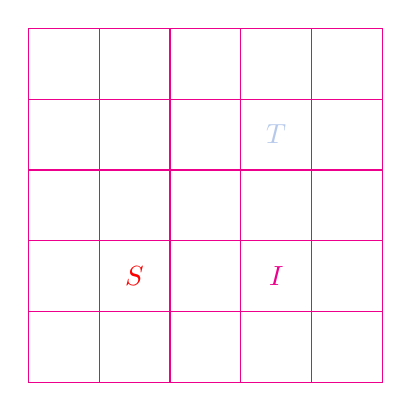
\begin{tikzpicture}[scale=0.9, toancuabi]
		\draw (0,0) grid (5,5);
		\draw (1.5,1.5) node{$\color{red}S$};
		\draw (3.5,1.5) node{$I$};
		\draw (3.5,3.5) node{$\color{cackithi!40}T$};
	\end{tikzpicture}
	\vspace*{-5pt}
	\end{figure}
	Now suppose that $S$ and $T$ are in different rows and columns. Let $I$ denote the person who is in the same row as $S$ and also in the same column as $T$. By definition, $T$ is shorter than $I$ and $S$ is taller than $I$. Therefore $T$ is shorter than $S$.
	\vskip 0.1cm
	In both cases, we see that $S$ is taller than $T$.
	\vskip 0.2cm
	\PIbox{{\color{toancuabi}\textbf{\color{toancuabi}Example} (How many ways to form the name?)}
	\vskip 0.1cm
	Thanh filled a triangle of squares with the letters of her name, as shown below.
	She counted all the $5-$letter paths that form her name T--H--A--N--H,
	each starts from the T letter in the middle of the bottom row,
	then goes left, right, or up. An example is also shown in the diagram.
	What number did she get?}
	\vskip 0.2cm
	\begin{figure}[H]
		\vspace*{-5pt}
		\centering
		\captionsetup{labelformat= empty, justification=centering}
		\renewcommand{\arraystretch}{1.2}
		\begin{tabular}{ccccccccc}
		&   &   &   & H                                                &                                                  &                                                  &   &   \\
		&   &   & H & N                                                & H                                                &                                                  &   &   \\
		&   & H & N & A                                                & \cellcolor{cackithi!40}N & \cellcolor{cackithi!40}H &   &   \\
		& H & N & A & \cellcolor{cackithi!40}H& \cellcolor{cackithi!40}  A  & N                                                & H &   \\
		H & N & A & H & \cellcolor{cackithi!40}T & H                                                & A                                                & N &  H 
	\end{tabular} 
	\vspace*{-10pt}
	\end{figure}
	\textit{Solution.}
	Consider the \textit{``half"} triangle shown in the diagram below.
	It is easy to see that in each path, there are two choices at each steps.
	One example is shown in the figure, when two As can be chosen after a choice of $H$.
	\begin{figure}[H]
	\vspace*{-5pt}
	\centering
	\captionsetup{labelformat= empty, justification=centering}
	\renewcommand{\arraystretch}{1.2}
	\begin{tabular}{ccccl}
		&   &                                                  &                                                  &  H                                                 \\
		&   &                                                  &  H                                                 &  N                                                 \\
		&   &  H                                                 &  N                                                 &  A                                                 \\
		&  H  &  N                                                 & \cellcolor{toancuabi!40}  A &  H                                                 \\
		H  &  N  & \cellcolor{toancuabi!40}  A  & \cellcolor{cackithi!40}  H  & \cellcolor{cackithi!40}  T 
	\end{tabular}
	\vspace*{-10pt}
	\end{figure}
	Therefore there are $2^4=16$ paths for a half triangle.
	In total there are $2\cdot 16-1=31$ choices,
	because the vertical path formed by all the squares in the $T$ column
	is shared by both half triangles.
	\vskip 0.1cm
	Thus, the number that Thanh got is $31.$
	\vskip 0.1cm
	\PIbox{{\color{toancuabi}\textbf{\color{toancuabi}Example} (What would be the largest number?)}
	\vskip 0.1cm
	In each square of an $n \times n$ chess board ($n \ge 4$),
	Antoine writes a number according to the following rules:
	\vskip 0.1cm
	$(1)$ The number in each square is one of $1,2,\ldots,n^2$.
	\vskip 0.1cm
	$(2)$ The two numbers in two neighbouring squares differ less than $3$.
	\vskip 0.1cm
	$(3)$ The number $3$ is written in one of the squares.
	\vskip 0.1cm
	What is the biggest number can Antoine write on the board?}
	\vskip 0.2cm
	\textit{Solution.}
	Let $m$ be the biggest number that can be written on the board.
	\begin{figure}[H]
	\vspace*{-5pt}
	\centering
	\captionsetup{labelformat= empty, justification=centering}
	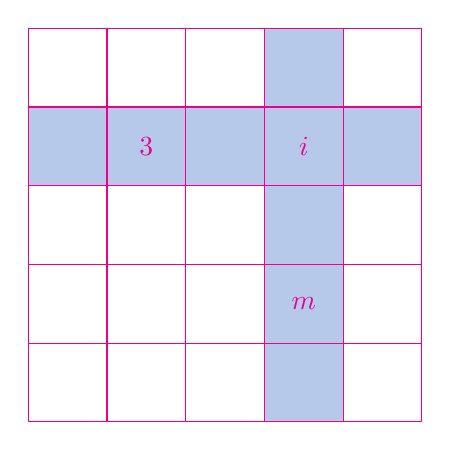
\begin{tikzpicture}[toancuabi]
			\filldraw[cackithi!40] (0,3) rectangle (5,4);
			\filldraw[cackithi!40] (3,0) rectangle (4,5);
			\draw (0,0) grid (5,5);
			\draw (1.5,3.5) node {$3$};
			\draw (3.5,1.5) node {$m$};
			\draw (3.5,3.5) node {$i$};
	\end{tikzpicture}
	\vspace*{-10pt}
	\end{figure}
	In the figure above, there are at most $(n-1)$ squares on the row of $3$,
	not including the square containing $3$, 
	from the number $3$ to the intersection $i$ with the column of $m$.
	Similarly there are at most $(n-1)$ squares on the column of $m$,
	not including the square containing $m$, 
	from the intersection $i$ with the row of $3$ to the number $m$.
	Thus the difference between $m$ and $3$ cannot be more than
	$2\cdot (n-1)+ 2\cdot (n-1)=4(n-1)$.
	\vskip 0.1cm
	Therefore, the biggest possible value of $m$ is $3+4(n-1)={4n-1.}$
	\vskip 0.2cm
	\PIbox{{\color{toancuabi}\textbf{\color{toancuabi}Example} (Colouring the paths)}
	\vskip 0.1cm
	In the $4 \times 4$ grid below, each cell at row $i$ and column $j$ contains the value equal to $i \times j.$
	A \textit{path} in the grid is a sequence of squares,
	such that consecutive squares share an edge and no square occurs twice in the sequence.
	Furthermore, the \textit{score} of a path is the sum of the values of all squares in the path.
	\vskip 0.1cm
	Determine the highest possible score of a path that begins at the bottom left corner of the grid 
	(where the number $1$ stands) and ends at the top right corner (where the number $16$ stands).}
	\vskip 0.2cm
	\begin{figure}[H]
	\vspace*{-5pt}
	\centering
	\captionsetup{labelformat= empty, justification=centering}
	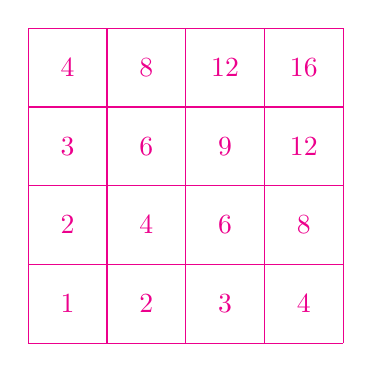
\begin{tikzpicture}[toancuabi]
		\draw (0,0) grid (4,4);
		\draw (0.5 , 0.5) node {$1$};
		\draw (0.5 , 1.5) node {$2$};
		\draw (0.5 , 2.5) node {$3$};
		\draw (0.5 , 3.5) node {$4$};
		\draw (1.5 , 0.5) node {$2$};
		\draw (1.5 , 1.5) node {$4$};
		\draw (1.5 , 2.5) node {$6$};
		\draw (1.5 , 3.5) node {$8$};
		\draw (2.5 , 0.5) node {$3$};
		\draw (2.5 , 1.5) node {$6$};
		\draw (2.5 , 2.5) node {$9$};
		\draw (2.5 , 3.5) node {$12$};
		\draw (3.5 , 0.5) node {$4$};
		\draw (3.5 , 1.5) node {$8$};
		\draw (3.5 , 2.5) node {$12$};
		\draw (3.5 , 3.5) node {$16$};
	\end{tikzpicture}
	\vspace*{-10pt}
	\end{figure}
	\textit{Solution.}
	Let us colour the squares of the grid with a chessboard pattern of black and white,
	starting with black in the bottom left--hand corner, as show below on the left diagram.
	A path in the grid will alternate between black and white squares,
	beginning and ending on black.
	Therefore, no path contains all the $8$ white squares.
	\vskip 0.1cm
	\begin{figure}[H]
		\vspace*{-5pt}
		\centering
		\captionsetup{labelformat= empty, justification=centering}
		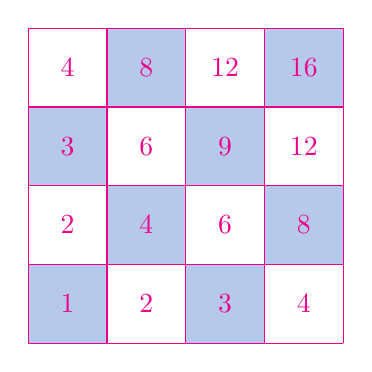
\begin{tikzpicture}[toancuabi]
			\foreach \y in {0,2}{
			\foreach \x in {0,2}{
					\fill[cackithi!40] (\x,\y) rectangle (1+\x,1+\y) rectangle (2+\x,2+\y);}}
			\draw (0,0) grid (4,4);
			\draw (0.5 , 0.5) node {$1$};
			\draw (0.5 , 1.5) node {$2$};
			\draw (0.5 , 2.5) node {$3$};
			\draw (0.5 , 3.5) node {$4$};
			\draw (1.5 , 0.5) node {$2$};
			\draw (1.5 , 1.5) node {$4$};
			\draw (1.5 , 2.5) node {$6$};
			\draw (1.5 , 3.5) node {$8$};
			\draw (2.5 , 0.5) node {$3$};
			\draw (2.5 , 1.5) node {$6$};
			\draw (2.5 , 2.5) node {$9$};
			\draw (2.5 , 3.5) node {$12$};
			\draw (3.5 , 0.5) node {$4$};
			\draw (3.5 , 1.5) node {$8$};
			\draw (3.5 , 2.5) node {$12$};
			\draw (3.5 , 3.5) node {$16$};
		\end{tikzpicture}
		\caption{\small\textit{\color{toancuabi}Figure $1$. Alternate colouring.}}
		\vspace*{-5pt}
	\end{figure}
	\begin{figure}[H]
	\vspace*{5pt}
	\centering
	\captionsetup{labelformat= empty, justification=centering}
	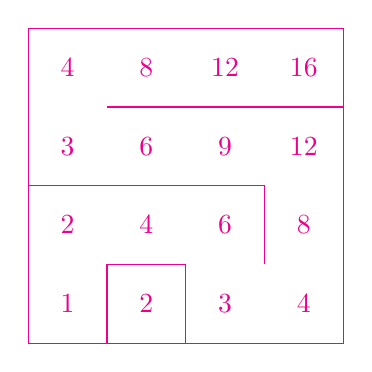
\begin{tikzpicture}[toancuabi]
		\draw (0,0) rectangle (4,4);
		\draw (1,0) grid (2,1);
		\draw (0,2) -- (3,2) -- (3,1);
		\draw (1,3) -- (4,3);
		\draw (0.5 , 0.5) node {$1$};
		\draw (0.5 , 1.5) node {$2$};
		\draw (0.5 , 2.5) node {$3$};
		\draw (0.5 , 3.5) node {$4$};
		\draw (1.5 , 0.5) node {$2$};
		\draw (1.5 , 1.5) node {$4$};
		\draw (1.5 , 2.5) node {$6$};
		\draw (1.5 , 3.5) node {$8$};
		\draw (2.5 , 0.5) node {$3$};
		\draw (2.5 , 1.5) node {$6$};
		\draw (2.5 , 2.5) node {$9$};
		\draw (2.5 , 3.5) node {$12$};
		\draw (3.5 , 0.5) node {$4$};
		\draw (3.5 , 1.5) node {$8$};
		\draw (3.5 , 2.5) node {$12$};
		\draw (3.5 , 3.5) node {$16$};
	\end{tikzpicture}
	\caption{\small\textit{\color{toancuabi}Figure $2$. Path with maximal value.}}
	\vspace*{-10pt}
	\end{figure}
	The path from $1$ to $16$ with the highest possible score should contain all the squares
	except for the square containing $2$ in the bottom row, as shown in the Figure $2$.
	The sum of the values of all the squares in this path is 
	\begin{align*}
		&(1\!+\!2\!+\!3\!+\!4)\!+\!(2\!+\!4\!+\!6\!+\!8)\\
		&\!+\!(3\!+\!6\!+\!9\!+\!12)\!+\!(4\!+\!8\!+\!12\!+\!16) \\
		= \,&(1\!+\!2\!+\!3\!+\!4)(1\!+\!2\!+\!3\!+\!4) \!=\! 10^2 \!=\! 100,
	\end{align*}		
	Thus, the highest possible score is $100-2={98}.$
	\vskip 0.2cm
	\PIbox{
	\centerline{\textbf{\color{toancuabi}Vocabulary}}
	\vskip 0.2cm
	{\color{toancuabi}path (n):} đường đi
	\vskip 0.1cm
	{\color{toancuabi}grid (n):} lưới
	\vskip 0.1cm
	{\color{toancuabi}board (n):} bàn cờ
	\vskip 0.1cm
	{\color{toancuabi}neighbouring squares (n):} các ô vuông kề nhau
	\vskip 0.1cm
	{\color{toancuabi}score (n):} số điểm
	}
\end{multicols}
\vspace*{-10pt}
{\color{toancuabi}\rule{1\linewidth}{0.1pt}}
\begin{center}
	\LARGE\textbf{\color{toancuabi}LỜI GIẢI, ĐÁP ÁN}
\end{center}
\begin{multicols}{2}
	\textbf{\color{toancuabi}Cuộc điều tra với những chữ số}
	\vskip 0.1cm
	Do tất cả các nhân viên trung thực đều viết đúng số lượng, chỉ sử dụng các chữ số $3$, $5$ hoặc $7$, suy ra ta chỉ cần xét $9$ trường hợp đối với số lượng các nhân viên trung thực: 
	\begin{align*}
				33,35,37,53,55,57,73,75,77.
			\end{align*}
	Chữ số $3$ được viết $33$ lần. Vì thế, số người trung thực không thể là $33$ (vì nếu không những người trung thực sẽ viết ra chữ số $3$ tận $66$ lần). Cũng vậy số người trung thực không thể là $35$, $37$, $53$ hoặc $73$, vì nếu không những người trung thực sẽ viết ra chữ số $3$ nhiều hơn $33$ lần.
	\vskip 0.1cm
	Chữ số $5$ được viết ra $66$ lần. Do  đó, số người trung thực không thể là $55$ (vì nếu không họ sẽ viết ra tận $110$ lần chữ số $5$), và cũng không thể là $75$ (vì nếu không, những người trung thực sẽ viết ra $75$ lần chữ số $5$).
	\vskip 0.1cm
	Số những người trung thực cũng không thể là $77$, vì nếu không những người trung thực sẽ viết ra $154$ lần chữ số $7$. 
	\vskip 0.1cm
	Còn lại duy nhất một khả năng là có $57$ người trung thực. Có rất nhiều trường hợp có thể xảy ra tương ứng với đáp số này, các em không nhất thiết phải tìm ra cụ thể tất cả các trường hợp.
	\vskip 0.1cm
	Ví dụ, có $9$ người ranh mãnh cũng viết số $57$, trong số những người còn lại có $11$ người gồm cả những người nói dối và những người ranh mãnh sẽ viết trả lời là số $33$, còn $11$ người (gồm cả những người nói dối và những người ranh mãnh) viết trả lời là số $73$.
	\vskip 0.1cm
	\textbf{\color{toancuabi}Góc cờ}
	\vskip 0.1cm
	\textit{Hình} $4$: $\pmb{1)}$ M$5.7$ Tg$4/1$\quad $\pmb{2)}$ M$7/8$ Tg$4/1$\quad  $\pmb{3)}$ M$8/7$ X$8.3$\quad $\pmb{4)}$ Tg$5/1$  Tg$4.1$\quad  $\pmb{5)}$ M$7.8$ Tg$4/1$ \quad$\pmb{6)}$ M$8.7$ Tg$4.1$\quad $\pmb{7)}$ M$7/5$ Tg$4/1$\quad $\pmb{8)}$ M$5/7$ Tg$4.1$\quad $\pmb{9)}$ M$7/8$ Tg$4/1$\quad $\pmb{10)}$ M$8/7$ X$8/2$\quad $\pmb{11)}$ M$7/6$ $(1-0)$
	\vskip 0.1cm
	\textit{Hình} $5$: 
	$\pmb{1)}$ C$5-6$ Tg$4/1$\quad $\pmb{2)}$ T$1/3$ X$9-7$\quad  $\pmb{3)}$ P$3/8$ X$7/1$\quad $\pmb{4)}$ P$4-6$  X$7-4$\quad  $\pmb{5)}$ C$6.1$ Tg$4/1$\quad $\pmb{6)}$ C$6.1$ $(1-0)$
	\vskip 0.1cm
	\hfill (\textit{Xem tiếp trang} $60$)
\end{multicols}

	\newpage 
%	
%	\thispagestyle{empty}
%	\begingroup 
%	\AddToShipoutPicture*{\put(0,0){\includegraphics[width=19.3cm]{MV.pdf}}}
%	\centering
%	\vspace*{0cm}
%	\endgroup
%	\newpage	
%	\pagestyle{empty}
%	
	\setcounter{figure}{0}
	\thispagestyle{thachthuctoanhocnone}
\pagestyle{thachthuctoanhoc}
\everymath{\color{thachthuctoanhoc}}
\graphicspath{{../thachthuctoanhoc/pic/}}
\begingroup
\AddToShipoutPicture*{\put(0,616){\includegraphics[width=19.3cm]{../thachthuctoanhoc/bannerthachthuc}}}
\centering
\vspace*{4cm}
\endgroup
\vspace*{-8pt}
\begin{tBox}
	\begin{itemize}[leftmargin = 13pt, itemsep = 1.0pt] 
		\item Mỗi bài toán đề xuất (kèm theo lời giải) cần được nêu rõ là bài sáng tác hay bài sưu tầm.
		%		\item Mỗi bài toán đề xuất (kèm theo lời giải) cần được nêu rõ là bài sáng tác hay bài sưu tầm (nếu là bài sưu tầm, cần ghi rõ nguồn).
		\item Bài giải cho mỗi bài toán cần được trình bày trong một file riêng hoặc
		một tờ giấy riêng.
		\item  Người đề xuất bài toán hoặc gửi bài giải cho các bài toán trong mục ``Thách thức kỳ này" cần ghi rõ họ, đệm, tên và nơi làm việc/học tập, số điện thoại liên hệ. Nếu là học sinh (hoặc sinh viên) cần ghi rõ là học sinh lớp mấy (hoặc sinh viên năm thứ mấy).
		\item Các bài toán trong mục Thách thức kỳ này hướng tới các độc giả là học sinh phổ thông; được phân chia thành các mức độ $B$, $A$, và được sắp xếp theo độ khó tăng dần, theo đánh giá chủ quan của Ban biên tập. Các bài toán mức độ $B$ không đòi hỏi các kiến thức vượt quá chương trình môn Toán cấp THCS; các bài toán mức độ $A$ không đòi hỏi các kiến thức vượt quá chương trình môn Toán cấp THPT.
		\item Cách thức gửi bài toán đề xuất hoặc lời giải: gửi file thu được bằng cách scan, ảnh chụp (rõ nét) của bản viết tay, hoặc được soạn thảo bằng các phần mềm Latex, Word tới \url{bbt@pi.edu.vn} hoặc gửi qua đường bưu điện tới Tòa soạn (xem địa chỉ tại bìa $2$).
		\item Hạn gửi lời giải cho các bài toán P$731$--P$740$: trước ngày $15/10/2023$.
	\end{itemize}
\end{tBox}
\begin{center}
	\vspace*{-5pt}
	\textbf{\color{thachthuctoanhoc}\color{thachthuctoanhoc}\color{thachthuctoanhoc}THÁCH THỨC KỲ NÀY}
	\vspace*{-5pt}
\end{center}
\begin{multicols}{2}
	\setlength{\abovedisplayskip}{4pt}
	\setlength{\belowdisplayskip}{4pt}
	{\color{thachthuctoanhoc}{\usefont{T5}{qag}{b}{n} P731.}}
	(Mức $B$) Ghép $9$ hình vuông thành một hình chữ nhật như ở hình dưới đây. Biết rằng, hình vuông màu đen có cạnh bằng $1$. Tìm chiều dài và chiều rộng của hình chữ nhật.
	\begin{figure}[H]
		\vspace*{-5pt}
		\centering
		\captionsetup{labelformat= empty, justification=centering}
		\begin{tikzpicture}[thachthuctoanhoc,scale=0.15]
				\draw[fill=black] (0,0) rectangle (1,1);
				\draw  (0.,-9.)-- (9.,-9.);
				\draw  (9.,-9.)-- (9.,0.);
				\draw  (9.,0.)-- (0.,0.);
				\draw  (0.,0.)-- (0.,-9.);
				\draw  (1.,0.)-- (9.,0.);
				\draw  (9.,0.)-- (9.,8.);
				\draw  (9.,8.)-- (1.,8.);
				\draw  (1.,8.)-- (1.,0.);
				\draw  (-10.,-9.)-- (0.,-9.);
				\draw  (0.,-9.)-- (0.,1.);
				\draw  (0.,1.)-- (-10.,1.);
				\draw  (-10.,1.)-- (-10.,-9.);
				\draw  (-6.,1.)-- (1.,1.);
				\draw  (1.,1.)-- (1.,8.);
				\draw  (1.,8.)-- (-6.,8.);
				\draw  (-6.,8.)-- (-6.,1.);
				\draw  (-10.,1.)-- (-6.,1.);
				\draw  (-6.,1.)-- (-6.,5.);
				\draw  (-6.,5.)-- (-10.,5.);
				\draw  (-10.,5.)-- (-10.,1.);
				\draw  (-6.,8.)-- (9.,8.);
				\draw  (9.,8.)-- (9.,23.);
				\draw  (9.,23.)-- (-6.,23.);
				\draw  (-6.,23.)-- (-6.,8.);
				\draw  (-24.,-9.)-- (-10.,-9.);
				\draw  (-10.,-9.)-- (-10.,5.);
				\draw  (-10.,5.)-- (-24.,5.);
				\draw  (-24.,5.)-- (-24.,-9.);
				\draw  (-24.,5.)-- (-6.,5.);
				\draw  (-6.,5.)-- (-6.,23.);
				\draw  (-6.,23.)-- (-24.,23.);
				\draw  (-24.,23.)-- (-24.,5.);	
		\end{tikzpicture}
		\vspace*{-10pt}
	\end{figure} 
	\begin{flushright}
		\textit{Bùi Văn Biên, France (st)}
	\end{flushright}
	{\color{thachthuctoanhoc}{\usefont{T5}{qag}{b}{n} P732.}}
	(Mức $B$) Xét $4$ số thực (không nhất thiết đôi một khác nhau), mà mỗi số có trị tuyệt đối không vượt quá $\dfrac12$, và tổng của ba số bất kỳ, trong bốn số đó, là một số nguyên. Tìm tất cả các giá trị có thể của tổng bốn số đó.
	\begin{flushright}
		\textit{Nguyễn Đức Tấn, Tp. Hồ Chí Minh (st)}
	\end{flushright}
	{\color{thachthuctoanhoc}{\usefont{T5}{qag}{b}{n} P733.}}
	(Mức $B$) Tìm giá trị nhỏ nhất của biểu thức
	\begin{align*}
		S=\left[\dfrac{b+c}a\right]+\left[\dfrac{c+a}b\right]+\left[\dfrac{a+b}c\right]
	\end{align*}
	trong đó $a,b,c$ là các số nguyên dương.
	\begin{flushright}
		\textit{Nguyễn Việt Hùng, Hà Nội}
	\end{flushright}
	
	{\color{thachthuctoanhoc}{\usefont{T5}{qag}{b}{n} P734.}}
	(Mức $B$) Cho hình vuông $ABCD$. Gọi $E$ là trung điểm của $AD$; $H$ là hình chiếu vuông góc của $B$ trên $CE$. Trên đường chéo $AC$, lấy điểm $M$ sao cho $AM=\frac38AC$. Chứng minh rằng, $ME$ song song với $DH$.  
	\begin{center}
		\definecolor{ffvvqq}{rgb}{1,0.3333333333333333,0}
		\definecolor{qqzzcc}{rgb}{0,0.6,0.8}
		\definecolor{qqqqff}{rgb}{0,0,1}
		\definecolor{qqqqffa}{rgb}{1,1,1}
		\begin{tikzpicture}[thachthuctoanhoc,scale=0.75]
			\draw [color=qqzzcc] (-3.3,3.3)-- (2.7,3.3);
			\draw [color=qqzzcc] (-3.3,3.3)-- (-3.3,-2.7);
			\draw [color=qqzzcc] (-3.3,-2.7)-- (2.7,-2.7);
			\draw [color=qqzzcc] (2.7,-2.7)-- (2.7,3.3);
			\draw  (-3.3,0.3)-- (2.7,-2.7);
			\draw  (0.3,-1.5)-- (2.7,3.3);
			\draw  (-3.3,-2.7)-- (0.3,-1.5);
			\draw [color=ffvvqq] (-3.3,3.3)-- (2.7,-2.7);
			\draw  (-3.3,0.3)-- (-1.05,1.05);
			\draw [fill=white] (-3.3,3.3) circle (1.6pt);
			\draw (-3.44,3.79) node {$A$};
			\draw [fill=white] (2.7,3.3) circle (1.6pt);
			\draw (2.72,3.71) node {$B$};
			\draw [fill=white] (2.7,-2.7) circle (1.6pt);
			\draw (2.68,-3.05) node {$C$};
			\draw [fill=white] (-3.3,-2.7) circle (1.6pt);
			\draw (-3.36,-3.09) node {$D$};
			\draw [fill=white] (-3.3,0.3) circle (1.6pt);
			\draw (-3.76,0.47) node {$E$};
			\draw [fill=white] (0.3,-1.5) circle (1.6pt);
			\draw (0.3,-1.85) node {$H$};
			\draw [fill=white] (-1.05,1.05) circle (1.6pt);
			\draw (-0.76,1.49) node {$M$};
		\end{tikzpicture}
	\end{center}
	\begin{flushright}
		\textit{Huỳnh Thanh Hưng, Phú Yên}
	\end{flushright}
	{\color{thachthuctoanhoc}{\usefont{T5}{qag}{b}{n} P735.}}
	(Mức $B$) Tìm tất cả các số nguyên dương $n$, để $n!+n$ là một luỹ thừa với số mũ nguyên dương của một số nguyên tố.
	\begin{flushright}
		\textit{Hà Duy Hưng, Hà Nội}
	\end{flushright}
	{\color{thachthuctoanhoc}{\usefont{T5}{qag}{b}{n} P736.}}
	(Mức $B$) Bạn An có $8$ quả cân có tổng trọng lượng là $16$ kg và trọng lượng mỗi quả, theo đơn vị kg, là một số nguyên dương không vượt quá $8$. Chứng minh rằng, có thể chia $8$ quả cân này thành hai nhóm sao cho các tổng trọng lượng của các quả cân cùng nhóm bằng nhau.
	\begin{flushright}
		\textit{Tường Thanh, Nghệ An}
	\end{flushright}
	{\color{thachthuctoanhoc}{\usefont{T5}{qag}{b}{n} P737.}}
	(Mức $A$) Xét các số thực dương $a,b,c$,  thoả mãn $a^2+b^2+c^2=1$. Tìm giá trị nhỏ nhất của biểu thức
	\begin{align*}
		S=2\left(a^3+b^3+c^3\right)-\left(a+b+c\right).
	\end{align*}
	\begin{flushright}
		\textit{Kiều Đình Minh, Phú Thọ}
	\end{flushright}
	{\color{thachthuctoanhoc}{\usefont{T5}{qag}{b}{n} P738.}}
	(Mức $A$) Cho tam giác $ABC$ ngoại tiếp đường tròn $(I)$. Gọi $J$ là tâm đường tròn bàng tiếp góc $A$ của tam giác đó. Trên cạnh $BC$, lấy điểm $D$ tùy ý, sao cho ba điểm $A,I,D$ không thẳng hàng. Đường thẳng $AD$ cắt các đường thẳng $IB, IC$, tương ứng, tại $E,F$. Gọi $H$ là trực tâm của tam giác $IEF$, và gọi $K$ là trung điểm của $AD$. Chứng minh ba điểm $K, H, J$ thẳng hàng.
	\begin{center}
		\definecolor{ffvvqq}{rgb}{1,0.3333333333333333,0}
		\definecolor{qqzzcc}{rgb}{0,0.6,0.8}
		\definecolor{qqqqff}{rgb}{0,0,1}
		\definecolor{qqqqffa}{rgb}{1,1,1}
		\definecolor{cqcqcq}{rgb}{0.7529411764705882,0.7529411764705882,0.7529411764705882}
		\begin{tikzpicture}[thachthuctoanhoc,scale=0.45]
			\draw [color=qqzzcc] (-3.679901022761026,4.943589529660562)-- (-4.58,-1.6);
			\draw [color=qqzzcc] (-4.58,-1.6)-- (3.08,-1.6);
			\draw [color=qqzzcc] (3.08,-1.6)-- (-3.679901022761026,4.943589529660562);
			\draw [color=ffvvqq] (-3.257494355051633,-1.6)-- (-3.679901022761026,4.943589529660562);
			\draw [color=ffvvqq] (-4.58,-1.6)-- (-2.151513063456181,0.5173053476685014);
			\draw [color=ffvvqq] (-3.4275087350979017,1.0337281160719551)-- (3.08,-1.6);
			\draw [dashed] (-3.4686976889063295,1.671794764830281)-- (0.6515130634561829,-7.600391557576506);
			\draw  (-2.151513063456181,0.5173053476685014) circle (2.117305347668501cm);
			\draw  (0.6515130634561829,-7.600391557576506) circle (6.000391557576506cm);
			\draw [color=qqzzcc] (-4.58,-1.6)-- (-5.292904303746716,-6.782711296880436);
			\draw [color=qqzzcc] (3.08,-1.6)-- (4.824890183355734,-3.2890550757724784);
			\draw [fill=white] (-3.679901022761026,4.943589529660562) circle (2.5pt);
			\draw (-3.7075216945790075,5.430778676473025) node {$A$};
			\draw [fill=white] (-4.58,-1.6) circle (2.5pt);
			\draw (-5.171417300932007,-1.6163200271099578) node {$B$};
			\draw [fill=white] (3.08,-1.6) circle (2.5pt);
			\draw (3.5014736499140704,-1.2848719652941842) node {$C$};
			\draw [fill=white] (-2.151513063456181,0.5173053476685014) circle (2.5pt);
			\draw (-1.9397986982282145,0.012402451962288) node {$I$};
			\draw [fill=white] (0.6515130634561829,-7.600391557576506) circle (2.5pt);
			\draw (0.6565444526620129,-8.41453873427639) node {$J$};
			\draw [fill=white] (-3.257494355051633,-1.6) circle (2.5pt);
			\draw (-3.3484529609452527,-2.058250776197656) node {$D$};
			\draw [fill=white] (-3.4686976889063295,1.671794764830281) circle (2.5pt);
			\draw (-2.80379702736733282,1.9124706683174956) node {$K$};
			\draw [fill=white] (-3.327960493319134,-0.5083943985466047) circle (2.5pt);
			\draw (-2.84462557094746,-0.667344980266746) node {$E$};
			\draw [fill=white] (-3.4275087350979017,1.0337281160719551) circle (2.5pt);
			\draw (-3.818004381850932,0.9800231237802691) node {$F$};
			\draw [fill=white] (-2.9332617149580074,0.4668413261447786) circle (2.5pt);
			\draw (-2.685556837313705,0.8842990928723823) node {$H$};
			\draw [fill=white] (0.6515130634561829,-1.6) circle (2.5pt);
			\draw [fill=white] (-5.292904303746716,-6.782711296880436) circle (2.5pt);
			\draw [fill=white] (4.824890183355734,-3.2890550757724784) circle (2.5pt);
		\end{tikzpicture}
	\end{center}
	\begin{flushright}
		\textit{Lưu Công Đông, Hà Nội}
	\end{flushright}
	{\color{thachthuctoanhoc}{\usefont{T5}{qag}{b}{n} P739.}}
	(Mức $A$) Cho dãy số $(a_n)$, xác định bởi
	\begin{align*}
		a_n=\left[\dfrac n{\sqrt2}\right]+\left[\dfrac n{\sqrt3}\right],\quad\text{với mọi $n\in\mathbb N^*$}.
	\end{align*}
	Chứng minh rằng, trong dãy $(a_n)$ chứa vô hạn số chẵn và vô hạn số lẻ.
	\begin{flushright}
		\textit{Nguyễn Tiến Lâm, Hà Nội}
	\end{flushright}
	{\color{thachthuctoanhoc}{\usefont{T5}{qag}{b}{n} P740.}}
	(Mức $A$) Cho bảng ô vuông kích thước $2023\times 2023$. Tìm số nguyên dương $n$ nhỏ nhất, sao cho có thể đặt $n$ viên bi vào các ô vuông con của bảng, đảm bảo các điều kiện sau được đồng thời thoả mãn:
	\vskip 0.1cm
	$i/$ Ở mỗi ô vuông con chỉ có tối đa một viên bi;
	\vskip 0.1cm
	$ii/$ Với mỗi ô vuông con không có bi, tổng số viên bi ở hàng và cột chứa ô đó không nhỏ hơn $2023$.
	\begin{flushright}
		\textit{Tô Trung Hiếu, Nghệ An (st)}
	\end{flushright}
\end{multicols}
%\newpage
%\centerline{{\large{\textbf{\color{thachthuctoanhoc}GIẢI BÀI KỲ TRƯỚC}}}}
%\vspace*{-5pt}
%\begin{multicols}{2}
%\end{multicols}	
	\newpage 

	\setcounter{figure}{0}
	\thispagestyle{hoccungpinone}
\pagestyle{hoccungpi}
\everymath{\color{hoccungpi}}
\graphicspath{{../hoccungpi/pic/}}
%\blfootnote{$^{1}$\color{hoccungpi}Đại học Bách Khoa Hà Nội.}
\begingroup
\AddToShipoutPicture*{\put(0,616){\includegraphics[width=19.3cm]{../bannerhoccungpi}}}
\AddToShipoutPicture*{\put(90,555){\includegraphics[scale=1]{../tieude.pdf}}}
\centering
\endgroup
\vspace*{155pt}

\begin{multicols}{2}
	$\pmb{1.}$ \textbf{\color{hoccungpi}Đa thức và hàm đa thức} 
	\vskip 0.1cm
	$\pmb{1.1.}$ \textbf{\color{hoccungpi}Đa thức.}
	Đa thức là một biểu thức đại số nhận được một cách hình thức từ các { biến số} và các { hệ số} thông qua các phép tính cộng, trừ và nhân. 
	\vskip 0.1cm
	Các hệ số là phần tử thuộc một tập hợp nào đó, thông thường là một tập hợp số (ví dụ $\mathbb {Z, Q, R, C}$) nhưng cũng có thể là một tập tổng quát hơn mà trên đó đã xác định các phép toán cộng, trừ, nhân. 
	\vskip 0.1cm
	Biến số là các ký tự hình thức (ví dụ $x,y,X,Y,...$) mà ta có thể thay thế chúng bằng những phần tử trong tập hợp chứa các hệ số hoặc một tập hợp lớn hơn mà trên đó cũng xác định các phép toán cộng, trừ và nhân.
	\vskip 0.1cm
	Đa thức một biến có thể được mô tả bằng biểu thức dạng
	\begin{align*}
		P(x)=a_0x^n+a_1x^{n-1}+\ldots+a_n.
	\end{align*}
	Như vậy thông tin về các đa thức một biến bao gồm hai loại: số tự nhiên $n$ được gọi là bậc của nó, ký hiệu là $\deg P(x)$, và các số (nguyên, hữu tỷ, thực hay phức) $a_0,a_1,\ldots, a_n$ -- các hệ số của nó. 
	\begin{tBox}
		Thông tin về đa thức một biến với bậc (không quá) $n$ là một dãy có thứ tự gồm $n+1$ {\em đơn vị thông tin}.
	\end{tBox}
	Dưới đây ta sẽ chỉ xét các { đa thức một biến} với hệ số nằm trong một tập số như $\mathbb{Q, R, C}$. 
	\vskip 0.1cm	
	$\pmb{1.2.}$ \textbf{\color{hoccungpi}Phép chia có dư.}  
	Đối với đa thức hệ số thực ta có thể thực hiện được phép chia có dư, tương tự như đối với các số nguyên. Cho các đa thức $P(x)$ và $Q(x)$ với $Q(x)\neq 0$, khi đó tồn tại duy nhất các đa thức $P_1(x)$ và $R(x)$ với $\deg R(x)<\deg Q(x)$ sao cho
	\begin{align*}
		P(x)= Q(x)P_1(x)+R(x).
	\end{align*}
	Ta nói đa thức $P(x)$ chia hết cho đa thức $Q(x)$ nếu $R(x)=0$.   
	\vskip 0.1cm
	\textbf{\color{hoccungpi}Chú ý}. Ta có thể thay thế điều kiện ``hệ số thực" bởi điều kiện ``hệ số phức" hay ``hệ số hữu tỷ". Nhưng ta không thể áp dụng với điều kiện ``hệ số nguyên". 
	\vskip 0.1cm
	Ví dụ, ta không thể thực hiện được phép chia có dư của đa thức $x^2+1$ cho đa thức $2x$ {trong tập hợp đa thức hệ số nguyên}!
	\vskip 0.1cm
	$\pmb{1.3.}$ \textbf{\color{hoccungpi}Hàm đa thức.}
	Xét các đa thức một biến với hệ số nằm trong một tập số. Khi đó, bằng cách thay thế biến số bằng các giá trị trong tập số đó ta thu được một hàm số. Hàm số thu được bằng cách này gọi là {hàm đa thức}. Chúng thường được mô tả ở dạng
	\begin{align*}
		y=P(x),
	\end{align*}
	trong đó $P(x)$ là một đa thức theo biến $x$.
	\vskip 0.1cm
	{Nguyên lý đồng nhất của Đại số học} nói rằng nếu hai hàm đa thức (trên tập số thực) bằng nhau tại mọi giá trị của biến số thì các đa thức xác định chúng bằng nhau. Nói cách khác, mỗi hàm đa thức được xác định bởi một đa thức duy nhất. 
	\vskip 0.1cm
	Ta chú ý rằng tính đúng đắn của nguyên lý này phụ thuộc vào miền giá trị của biến số (và hệ số). Ví dụ nguyên lý đồng nhất sai nếu xét đa thức trên tập các lớp đồng dư. 
	\vskip 0.1cm	
	$\pmb{1.4.}$ \textbf{\color{hoccungpi}Nghiệm của đa thức.}
	Nghiệm, hay còn gọi là không điểm, của một đa thức $P(x)$ là những giá trị của biến số $x$ mà tại đó $P(x)$ nhận giá trị $0$. Sử dụng phép chia có dư của $P(x)$ cho $x-a$ ta có
	\begin{align*}
		P(x)=(x-a)P_1(x)+P(a).
	\end{align*}
	Như vậy nếu $a$ là nghiệm của $P(x)$ thì $P(x)$ chia hết cho $x-a$. Từ đó ta kết luận một đa thức bậc $n$ { có không quá $n$ nghiệm}.
	\vskip 0.1cm
	{ Định lý cơ bản của Đại số học} khẳng định mọi đa thức với hệ số phức với bậc lớn hoặc bằng $1$ luôn có nghiệm phức. 
	Từ đó suy ra, một đa thức bậc $n\geq 1$ luôn có thể viết được ở dạng
	\begin{align*}
		P(x)=a_0\prod_{i=1}^n(x-x_i), \quad x_i\in\mathbb C.
	\end{align*}
	Chú ý rằng các số (phức) $x_i$ có thể bằng nhau -- trong trường hợp đó ta nói $P(x)$ có {\em nghiệm bội}.
	\begin{tBox}
		Nghiệm bội của một đa thức luôn là nghiệm chung của đa thức đó với đạo hàm của nó. 
	\end{tBox}
	$\pmb{1.5.}$ \textbf{\color{hoccungpi}Các tính chất cơ bản của đa thức dẫn tới nguyên lý nội suy.}
	\vskip 0.1cm
	-- Hai đa thức bằng nhau nếu chúng xác định hai hàm số  bằng nhau (trên các tập số nguyên, hữu tỷ, thực hay phức);
	\vskip 0.1cm
	-- Hai đa thức bằng nhau nếu giá trị chúng bằng nhau tại ``đủ nhiều giá trị của biến số'', phát biểu một cách tương đương là, một đa thức sẽ đồng nhất bằng $0$ nếu nó bằng $0$ tại ``đủ nhiều giá trị của biến số'';
	\vskip 0.1cm
	-- Một đa thức được xác định duy nhất bởi giá trị của nó tại ``đủ nhiều giá trị của biến số'', ``đủ nhiều'' được xác định là nhiều hơn bậc của đa thức. Ví dụ một tập vô hạn luôn là ``đủ nhiều''.
	\vskip 0.1cm
	$\pmb{2.}$ \textbf{\color{hoccungpi}Nội suy Lagrange}
	\vskip 0.1cm
	Bài toán nội duy Lagrange là xác định một đa thức bậc (không quá) $n-1$ từ các giá trị của đa thức tại $n$ vị trí khác nhau.
	\begin{tBox}
		\textbf{\color{hoccungpi}Bài toán nội suy Lagrange.}
		Cho các số $y_1,\ldots, y_n$ và các số phân biệt $x_1,\ldots,x_n$. Xác định đa thức $P(x)$ bậc không quá $n-1$ thỏa mãn:
		\begin{align*}
			P(x_i)=y_i, \text{ với mọi } i=1,2,\ldots, n.
		\end{align*}
	\end{tBox}
	\textbf{\color{hoccungpi}Nhận xét}.
	Nếu tồn tại đa thức $P(x)$ (với bậc không quá $n-1$) nhận giá trị $y_i$ tại điểm $x_i$, 
	$i=1,2,\ldots, n$, thì $P(x)$ là duy nhất. 
	Từ đó suy ra { tính chất tuyến tính} của bài toán nội suy Lagrage:
	\vskip 0.1cm
	-- Giả sử $Q(x)$ là đa thức được xây dựng từ bộ số $(z_1,\ldots, z_n):$
	\begin{align*}
		Q(x_i)=z_i,\quad i=1,\ldots,n,
	\end{align*}
	thì đa thức $P(x)+Q(x)$ được xác định từ bộ số
	\begin{align*}
		(y_1+z_1,\ldots,y_n+z_n).
	\end{align*}
	-- Bộ số $(\lambda y_1,\ldots,\lambda y_n)$ xác định đa thức $\lambda P(x)$ ($\lambda$ là một số bất kỳ).  
	\vskip 0.1cm
	{Trên cơ sở của tính chất tuyến tính, ta sẽ xây dựng đa thức $P(x)$ bắt đầu từ những bộ số $(y_1,\ldots,y_n)$ đơn giản nhất.} 
	\vskip 0.1cm
	-- Nếu tất cả các giá trị $y_i$ đều bằng $0$, ta có $P(x)=0$.
	\vskip 0.1cm  
	-- Nếu $y_1=1, y_2=\ldots=y_n=0$ thì đa thức $P_1(x)$ tương ứng sẽ nhận các giá trị  $x_2,\ldots,x_n$ làm nghiệm. Do $P_1(x)$ có bậc không quá $n-1$ nên  
	\begin{align*}
		P(x)=c(x-x_2)\ldots(x-x_n).
	\end{align*}
	Thay $x=x_1$ ta suy ra
	\begin{align*}
		c=\frac1{(x_1-x_2)\ldots(x_1-x_n)}.
	\end{align*}
	Từ đó
	\begin{align*}
		P_1(x)=\frac{ (x-x_2)\ldots(x-x_n)}{
			(x_1-x_2)\ldots(x_1-x_n)}.
	\end{align*}
	-- Tương tự, với bộ $y_1=\ldots=y_{i-1}=y_{i+1}=\ldots=y_n=0$, $y_i=1$,  đa thức tương ứng là 
	\begin{align*}
		P_i(x) =\prod_{j\neq i}\frac{(x-x_j)}{ (x_i-x_j)}.
	\end{align*}
	Theo nguyên lý tuyến tính nêu trên, ta có lời giải bài toán tổng quát như sau. Đa thức  
	\begin{align*}
		P(x)=\sum_{i=1}^n y_i\prod_{j\neq i}\frac{(x-x_j)}{ (x_i-x_j)} \tag{$1$}
	\end{align*}
	thỏa mãn $P(x_i)=y_i$.
	\vskip 0.1cm
	\textbf{\color{hoccungpi}Chú ý}. Bậc của $P(x)$  có thể bé hơn hẳn $n-1$.
	\vskip 0.1cm
	\textbf{\color{hoccungpi}Bài toán} $\pmb{2.1.}$ Giả sử $A, B$ và $C$ là phần dư của đa thức $P(x)$ khi chia cho $x-a,x-b$ và $x-c$.
		Tìm phần dư của phép chia đa thức đó cho $(x-a)(x-b)(x-c).$
	\vskip 0.1cm
	\textbf{\color{hoccungpi}Bài toán} $\pmb{2.2.}$ Chứng minh rằng nếu $f(x)$ là đa thức bậc nhỏ
		hơn $n$ thì phân thức
		\begin{align*}
			\frac{f(x)}{(x-x_1)(x-x_2)\ldots (x-x_n)}
		\end{align*}
		trong đó $x_1, x_2, \ldots, x_n$ là các giá trị khác nhau, 
		luôn biểu diễn được ở dạng
		\begin{align*}
			\frac{A_1}{x-x_1}+\frac{A_2}{x-x_2}+\ldots +\frac{A_n}{x-x_n}.
		\end{align*}
		với các số $  A_1, A_2,\ldots, A_n$ nào đó.
	\vskip 0.1cm
	\textbf{\color{hoccungpi}Bài toán} $\pmb{2.3.}$ Cho $x_1,\ldots,x_n$ là các số thực phân biệt. Đặt  $g(x):=\prod_{i=1}^n(x-x_i)$. Chứng minh rằng
	\begin{align*}
		\sum_i\frac{x_i^k}{g'(x_i)}= \begin{cases}
			0&\text{ với } k=0,1,\ldots,n-2;\\
			1& \text{ với } k=n-1.
		\end{cases}
	\end{align*}
	\textbf{\color{hoccungpi}Nhận xét.} Trong bài toán trên ta thực sự có các đồng nhất thức, nghĩa là ta có thể coi $x_i$ như là các biến số, tuy nhiên việc chứng minh trực tiếp đồng nhất thức này bằng các biến đổi đại số là rất phức tạp.  
	\vskip 0.1cm
	\textit{Lời giải.} 
	Lấy đạo hàm hai vế của đẳng thức 
	\begin{align*}
			g(x)=\prod_{i=1}^n(x-x_i)  \tag{$2$}
	\end{align*}
	ta thu được:
	\begin{align*}
		g'(x)=\sum_{i=1}^n\prod_{j\neq i}^n(x-x_j).
	\end{align*}  
	Từ đó
	\begin{align*}
		g'(x_i)=\prod_{j\neq i}(x_i-x_j). \tag{$3$}
	\end{align*}
	Áp dụng công thức nội duy Lagrange cho  đa thức $x^k$ ta thu được
	\begin{align*}
		x^k= \sum_{i=1}^nx_i^k\prod_{j\neq i}\frac{(x-x_j)}{ (x_i-x_j)}.
	\end{align*}
	So sánh hệ số của $x^{n-1}$ ở hai vế cho ta các hệ thức cần chứng minh cho $k\leq n-1$.
	\vskip 0.1cm
	\textbf{\color{hoccungpi}Bài toán} $\pmb{2.4.}$ Tính 
	\begin{align*}
		h_{k}:=\sum_i\frac{x_i^{n+k-1}}{g'(x_i)},
	\end{align*}
	với $k=1,2,3.$
	\vskip 0.1cm 
	\textit{Lời giải.} 
	Xét công thức Viète 
	\begin{align*}
		g(x)\!=\!\prod_{i=1}^n(x\!-\!x_i)\!=\!x^{n}\!-\!e_1x^n\!+\!\ldots\!+\!(\!-\!1)^{n}e_{n}.
	\end{align*}
	Các hệ số $e_i$ là các { đa thức đối xứng cơ bản} theo
	các biến $x_1,\ldots,x_n$. 
	\vskip 0.1cm
	Nhân theo vế đẳng thức $g(x_i)=0$ với $x_i^{k}$ ta thu được
	\begin{align*}
		x_i^{n+k}-e_1x_i^{n+k-1}+\ldots+(-1)^{n}e_{n}
		x_i^{k}=0.
	\end{align*}	
	{ Chia theo vế cho  $ \prod_{j\neq i}(x_i-x_j)$}
	và lấy tổng theo $i$, ta thu được 
	\begin{align*}
		h_{k+1}-e_1h_{k}+\ldots+(-1)^{n}e_{n}h_{k+1-n}=0,
	\end{align*}
	với quy ước { $h_0=1$ và $h_k=0$ nếu $k<0$.} 
	Công thức trên cho phép ta tính các đa thức $h_k$. 
	Cụ thể ta có: 
	\begin{align*}
		h_1=e_1&=\sum_i x_i\\
		h_2=e_1h_1-e_2&=\sum_{i\leq j}x_ix_j\\
		h_3=e_1h_2-e_2h_1+e_3&=\sum_{i\leq j\leq k}x_ix_jx_k.
	\end{align*}
	\textbf{\color{hoccungpi}Nhận xét}. Trong lời giải trên ta sử dụng hai kỹ thuật. Thứ nhất là thế $x=x_i$ vào $g(x)$ để thu được một hệ thức giữa  $x_i$ và các hệ số $e_j$. Thứ hai là nhân hệ thức đó theo các {trọng số}. 
	\vskip 0.1cm
	\textbf{\color{hoccungpi}Bài toán} $\pmb{2.5.}$  Chứng minh công thức tổng quát sau với mọi $k=4,5, \ldots$
	\begin{align*}
		h_k=\sum_{i_1\leq i_2\leq\ldots\leq i_k}x_{i_1}x_{i_2}\ldots x_{i_k}.
	\end{align*}
	Các đa thức $h_k$ được gọi là { \em đa thức đối xứng toàn phần} theo các biến $x_1,\ldots,x_n$.
	\vskip 0.1cm
	$\pmb{2.1.}$ \textbf{\color{hoccungpi}Hệ số của đa thức nhận được từ công thức nội suy Lagrange.}
	Trong bài tập $2.1$ ta đã sử dụng phương pháp so sánh hệ số trong công thức nội suy Lagrange. Một câu hỏi tự nhiên là: { có thể mô tả cụ thể được các hệ số của $P(x)$ từ các giá trị $y_i$ và $x_i$ hay không?}
	\vskip 0.1cm
	Từ đẳng thức
	\begin{align*}
		P(x)&= a_0x^{n-1}+a_1x^{n-2}+\ldots+a_{n-1} \\
		&= \sum_{i=1}^n y_i \frac{\prod_{j\neq i}^n(x-x_i)}{g'(x_i)}, \tag{$6$}
	\end{align*}
	so sánh hệ số ta thu được:
	\begin{align*}
		a_0= \sum_{i=1}^n 
		\frac{ y_i}{g'(x_i)} ,
	\end{align*}
	và 
	\begin{align*}
		a_1= \sum_{i=1}^n
		\frac{y_i (x_i-e_1)}{g'(x_i)}=
		\sum_{i=1}^n \frac{y_i  x_i}{g'(x_i)}-a_0e_1.
	\end{align*}
	\textbf{\color{hoccungpi}Bài toán} $\pmb{2.6.}$
	Đặt
	\begin{align*}
		b_k:=\sum_i\frac{y_i x_i^k}{g'(x_i)}.
	\end{align*}
	Chứng minh rằng các hệ số của đa thức $P(x)$ được tính bởi công thức
	\begin{align*}
		a_k=\sum_{j=0}^k(-1)^i e_jb_{k-j}.
	\end{align*}
	$\pmb{2.2.}$ \textbf{\color{hoccungpi}Đạo hàm bậc hai.} Trong các tính toán ở trên ta đã sử dụng các giá trị của đạo hàm bậc nhất của $g'(x)$. Vậy đạo hàm bậc hai có ý nghĩa gì? 
	\vskip 0.1cm
	\textbf{\color{hoccungpi}Bài toán} $\pmb{2.7.}$ Giả thiết rằng các số $x_i$ phân biệt, khi đó $g''(x_i)=0$ khi và chỉ khi
	\begin{align*}
		  \sum
		_{j\neq i}^n\frac1{x_i-x_j}=0.
	\end{align*}
	\textit{Lời giải.} 
	Tính đạo hàm hai lần của $g(x)$. Ta có
	\begin{align*}
		g''(x)=\sum_{k\neq  j}\prod_{i\neq k,j}(x-x_i)= \sum_{k\neq j}\frac{g(x)}{(x-x_k)(x-x_j)}.
	\end{align*}
	Từ đó ta có, với mỗi $1\leq i\leq n$: 
	\begin{align*}
		g''(x_i)=2\prod_{j\neq i}(x_i-x_j)\sum_{j\neq i}^n\frac1{x_i-x_j}.
	\end{align*}
	Vậy $g''(x_i)=0$ khi và chỉ khi
	\begin{align*}
		\sum_{j\neq i}\frac1{x_i-x_j}=0.
	\end{align*}  
	\textbf{\color{hoccungpi}Bài toán} $\pmb{2.8.}$
	Cho các số $0=x_0<x_1<\ldots<x_{n+1}=1$ thỏa mãn
	\begin{align*}
		\sum_{j=0,j\neq i}^{n+1}\frac1{x_i-x_j}=0,
	\end{align*}
	với mọi $i=1,2,\ldots,n$. Chứng minh rằng với mọi $i$, $x_i=1-x_{n+1-i}$.
	\vskip 0.1cm 
	$\pmb{3.}$ \textbf{\color{hoccungpi}Hàm sinh}
	\vskip 0.1cm
	Hàm sinh là một  công cụ dùng để phát biểu nhiều vấn đề của số học hay tổ hợp theo ngôn ngữ đại số, trên cơ sở đó sử dụng các phương pháp đại số (và giải tích) để giải quyết vấn đề. 
	\vskip 0.1cm
	Để xác định, hay tìm hiểu tính chất của một dãy số $a_0,a_1,\ldots$, thay vì nghiên cứu từng số hạng riêng rẽ, người ta tập hợp tất cả chúng trong một { \em tổng hình thức} hay một chuỗi lũy thừa:
	\begin{align*}
		A(x):=a_0+a_1 x+\ldots+ a_nx^n+\ldots.
	\end{align*}
	Nếu dãy đã cho hữu hạn, thì $A(x)$ là một đa thức. Như vậy các chuỗi lũy thừa có thể coi như một \textit{ khái niệm mở rộng của đa thức}.
	\vskip 0.1cm
	Tương tự như với đa thức, ta có thể quy ước các phép tính cộng, trừ hay nhân các hàm sinh.   
	\vskip 0.1cm
	Phép cộng và trừ được thực hiện theo thành phần (nghĩa là tương ứng với phép cộng, trừ hai dãy số).
	\vskip 0.1cm
	Phép nhân được thực hiện tương tự nhân đa thức. Với hai hàm sinh
	\begin{align*}
		A(t)=\sum_0^\infty a_ix^i,\quad B(t)=\sum_0^\infty b_i x^i,
	\end{align*}
	tích của chúng là hàm sinh $C(t)=\sum_0^\infty c_ix^i$, với các hệ số $c_i$ cho bởi công thức
	\begin{align*}
		c_i=\sum_{j=0}^i a_jb_{i-j}.
	\end{align*}
	$\pmb{3.1.}$ \textbf{\color{hoccungpi}Ví dụ.}
	\vskip 0.1cm
	-- Với
	\begin{align*}
		A(x)&=1-x,\\
		B(x)&=1+x+x^2+\ldots+x^n+\ldots
	\end{align*}
	ta có 
	\begin{align*}
		A(x)\cdot B(x)=1.
	\end{align*}
	Nghĩa là ta có đẳng thức
	\begin{align*}
		1+x+x^2+\ldots+x^n+\ldots=\frac 1{1-x}.
	\end{align*}
	Từ đó ta cũng có
	\begin{align*}
		B(x)^2&=1+2x+3x^2+\ldots+(n+1)x^n+\ldots\\
		&=\frac1{1-2x+x^2}.
	\end{align*}
	-- Hàm sinh cho dãy  các đa thức đối xứng cơ bản của $x_1,x_2,\ldots,x_n$ là: 
	\begin{align*}
		E(x)=1+e_1x+\ldots +e_nx^n=\prod_{i=1}^n (1+x_ix).
	\end{align*}   
	Xét hệ thức
	\begin{align*}
		&\frac 1{E(-x)}=\prod_i \frac 1{1-x_ix}\\
		=&\prod_i (1+x_i x+\ldots+x_i^nx^n+\ldots)\nonumber \\
		=& 1+h_1x+h_2x^2+\ldots+h_nx^n+\ldots  \tag{$7$}
	\end{align*} 
	\begin{align*}
		h_r=\sum_{i_1\leq\ldots\leq i_r}x_{i_1}\cdots x_{i_r}.
	\end{align*}
	-- Các đa thức  $h_r$ là các { đa thức đối xứng toàn phần} theo  $x_1,\ldots, x_n$. 
	Từ trên ta rút ra hệ thức sau giữa các đa thức $e_i$ và $h_i$:
	\begin{align*}
		&h_k-e_1h_{k-1}+\ldots+(-1)^ke_k=0,\\
		&\text{ với mọi }   1\leq k\leq n;\\
		&h_k-e_1h_{k-1}+\ldots+(-1)^ne_n h_{k-n}=0,\\
		&\text{ với mọi }    k\geq n.
	\end{align*}
	$\pmb{3.2.}$ \textbf{\color{hoccungpi}Đạo hàm của hàm sinh.}
	Ngoài các phép toán đại số nêu trên, ưu thế quan trọng của hàm sinh là ta có thể thực hiện phép {\em đạo hàm} trên chúng. 
	\vskip 0.1cm
	Nếu $A(x)=\sum a_nx^n$ thì 
	\begin{align*}
		A'(x):=\sum_{n=0}^\infty  (n+1)a_{n+1}x^n.
	\end{align*} 
	Bài tập dưới đây cho thấy hai phép toán định nghĩa như trên thỏa mãn các tính chất quen biết của phép toán đạo hàm và tích phân.
	\vskip 0.1cm
	\textbf{\color{hoccungpi}Bài toán} $\pmb{3.1.}$ Kiểm tra các hệ thức sau:
		\begin{align*}
			(A(t)\cdot B(t))'&=A(t)'\cdot B(t)+A(t)\cdot B(t)'\\
			\left(\frac 1{A(t)}\right)'&=-\frac{A(t)'}{A(t)^2}		
		\end{align*}
	\textbf{\color{hoccungpi}Bài toán} $\pmb{3.2.}$ Hàm mũ $\exp$ và hàm logarit $\ln$ được định nghĩa như sau:
	\begin{align*}
		\exp(x)=1+x+\ldots+\frac{x^n}{n!}+\ldots \tag{$8$}\\
		\ln(1\!+\!x)\!=\!x\!-\!\frac{x^2}2\!+\!\ldots\!+\!(\!-\!1)^n\frac{x^n}n\!+\!\ldots\! \tag{$9$}
	\end{align*}
	Chứng minh rằng
	\vskip 0.1cm
	-- $\exp(x)'=\exp(x)$, $\ln(x)'=\frac1{1+x}$;
	\vskip 0.1cm
	-- với mỗi hàm sinh $A(x)$ với hệ số đầu tiên bằng $0$, nghĩa là $A(0)=0$, thì $\exp(A(x))$ cũng là một hàm sinh;
	\vskip 0.1cm
	-- với mỗi hàm sinh $A(x)$với hệ số đầu tiên bằng $0$, nghĩa là $A(0)=1$, thì $\ln(A(x))$ cũng là một hàm sinh;
	\vskip 0.1cm
	-- $\exp(\ln(1+x))=1+x$, $\ln(\exp(x))=x$.
	\vskip 0.1cm
	$\pmb{4.}$ \textbf{\color{hoccungpi}Đa thức đối xứng} 
	\vskip 0.1cm
	Đa thức theo $n$ biến $x_1,x_2,\ldots,x_n$ được gọi là đối xứng nếu nó không thay đổi khi ta hoán vị các biến. Ta đã làm quen với các đa thức đối xứng sau: 
	\vskip 0.1cm
	-- Đa thức đối xứng cơ bản
	\begin{align*}
		e_r=\sum_{i_1<i_2<\ldots<i_r}x_{i_1}x_{i_2}\ldots x_{i_r},\quad r=1,2,\ldots, n.
	\end{align*}
	-- Đa thức đối xứng toàn phần
	\begin{align*}
		h _r=\sum_{i_1\le i_2\le \ldots \le i_r}x_{i_1}x_{i_2}\ldots x_{i_r},\quad r=1,2,\ldots,n.
	\end{align*}
	-- Ngoài ra ta còn đó tổng lũy thừa 
	\begin{align*}
		p_r=\sum_i x_i^r, r=1,2,\ldots
	\end{align*}
	Ứng với mỗi loại đa thức đối xứng ở trên ta sẽ xét hàm sinh của nó. Như ở phần trên ta có
	\begin{align*}
		E(x)&=\sum_{i=0}^n e_ix^i=\prod(1+x_ix),\\
		H(x)&=\sum_{i=0}^\infty h_i x^i=\prod\frac1{1-x_i x},\\
		P(x)&= \sum_{i=0}^\infty p_{i+1} x^{i}=\sum_{i=1}^n \frac {x_i}{1-x_i x}.
	\end{align*}	
	Từ hệ thức ($7$) ta có  $E(-x)\cdot H(x)=1$.
	\vskip 0.1cm
	Mặt khác, xét đạo hàm của $\ln E(x)$ ta có
	\begin{align*}
		\ln(E(x))'&=\frac{E'(x)}{E(x)}= \sum_i\ln\left({1+x_i x}\right)'\\
		&=\sum_i\frac{x_i}{1+x_i x}.
	\end{align*}
	Từ đó ta suy ra hệ thức:
	\begin{align*}
		E'(x)=E(x)\cdot P(-x).
	\end{align*}
	Đây chính là { hệ thức Newton} đối với các tổng lũy thừa.   
	So sánh hệ số của $x^{k}$ ở hai vế ta có.
	\vskip 0.1cm
	-- Với $0\leq k\leq n-1$:
	\begin{align*}
		(k+1)e_{k+1}=&e_kp_1-e_{k-1}p_2+\ldots\\
		&+(-1)^{k-1} e_1p_k+(-1)^{k}p_{k+1}
	\end{align*}
	hay là 
	\begin{align*}
		p_{k+1}=&e_1p_k+\ldots+(-1)^{k-1}e_kp_1\\
		&+(-1)^{k}(k+1)e_{k+1}.
	\end{align*}
	-- Với $k\geq n$:
	\begin{align*}
		0=&e_np_{k+1-n}-e_{n-1}p_{k+2-n}+\ldots\\
		&+(-1)^{n-1} e_1p_k+(-1)^{n}p_{k+1}
	\end{align*}
	hay là 
	\begin{align*}
		p_{k+1}=e_1p_k+\ldots+(-1)^{n-1}e_np_{k+1-n}.
	\end{align*}
	\textbf{\color{hoccungpi}Bài toán} $\pmb{4.1.}$ Chứng minh trực tiếp hệ thức Newton. 
			(Với trường hợp $k\geq n$, sử dụng phương pháp trong lời giải bài toán $2.4$. Với trường hợp $k<n$, sử dụng quy nạp theo số biến).
	\vskip 0.1cm
	\textbf{\color{hoccungpi}Bài toán} $\pmb{4.2.}$  Giả thiết $x_1,\ldots,x_n$ là các nghiệm (thực hoặc phức) của đa thức
	\begin{align*}
		x^n-{m\choose 1}x^{n-1}+\ldots+(-1)^n{m\choose n}
	\end{align*}
	với $m$ là số tự nhiên bất kỳ.
	Tính tổng
	\begin{align*}
		\sum x_i^k,\quad k=1,2,\ldots,n.
	\end{align*} 
	\textbf{\color{hoccungpi}Bài toán} $\pmb{4.3.}$
	Cho các số thực $a_1,\ldots,a_n$ và các số nguyên dương $b_1,\ldots,b_n$. Giả thiết tồn tại đa thức $f(x)$ sao cho:
	\begin{align*}
		(1-x)^nf(x)=1+\sum_i a_ix^{b_i}
	\end{align*}
	Tính $f(1)$ qua $b_i$ và $n$.
	\vskip 0.1cm
	$\pmb{5.}$ \textbf{\color{hoccungpi}Dãy cho bởi hệ thức truy hồi}
	\vskip 0.1cm
	Cho trước các số $e_1,e_2,\ldots,e_n$. Ta xét dãy vô hạn $(a_k)$, $k=0,1,\ldots$ các số thỏa mãn { hệ thức truy hồi}
	\begin{align*}
		&a_{n\!+\!k}\!=\!e_1a_{n\!+\!k\!-\!1}\!-\!e_2a_{n\!+\!k\!-\!2}\!+\!\ldots\!+\!(\!-\!1)^{n}e_na_k,\\
		&\quad k=0, 1,\ldots
	\end{align*}
	với các giá trị  $a_0,a_1,\ldots,a_{n-1}$ cho trước. 
	\vskip 0.1cm	
	-- Dãy $(a_n)$ được xác định duy nhất bởi hệ thức trên, và các số hạng
			$a_0, a_1,\ldots, a_{n-1}$ được gọi là {  điều kiện ban đầu}.
	\vskip 0.1cm  
	--	Bài toán xác định một dãy số thỏa mãn hệ thức truy hồi như trên còn được gọi là bài toán {\em giải phương trình sai phân}. 
	\vskip 0.1cm
	-- Đa thức 
	\begin{align*}
		g(x)=x^n-e_1x^{n-1}+\ldots+(-1)^n e_n
	\end{align*}
	được gọi là { đa thức đặc trưng} của phương trình trên.
	\vskip 0.1cm
	$\pmb{5.1.}$ \textbf{\color{hoccungpi}Nghiệm tổng quát.} 
	Việc xác định dãy từ hệ thức truy hồi và điều kiện ban đầu được thực hiện theo hai bước.
	\vskip 0.1cm
	--  Xác định tất cả các dãy thỏa mãn hệ thức truy hồi -- đây gọi là { các nghiệm tổng quát} của bài toán;
	\vskip 0.1cm
	--  Kết hợp với điều kiện ban đầu để xác định dãy cần tìm trong số các dãy ở trên -- đây gọi là { nghiệm riêng} của bài toán.
	\vskip 0.1cm	
	Gọi $t$ là một nghiệm của $g(x)$. Khi đó dãy $(\lambda t^k)_{k\geq 0}$
	thỏa mãn hệ thức truy hồi  ở trên, với mọi số $\lambda$.
	\vskip 0.1cm	
	Giả thiết $g(x)$ có $n$ { nghiệm phân biệt} $x_1,\ldots,x_n$ (có thể là nghiệm phức). Khi đó với mọi bộ số $\lambda_1,\ldots, \lambda_n$, dãy $(a_k)$ cho bởi
	\begin{align*}
		a_k=\sum_{i=1}^n \lambda_i x_i^k
	\end{align*}
	thỏa mãn hệ thức truy hồi ở trên.
	\vskip 0.1cm	
	$\pmb{5.2.}$ \textbf{\color{hoccungpi}Nghiệm riêng.}
	Các hệ số $\lambda_i$ được tính cụ thể thông qua điều kiện ban đầu $a_0,\ldots,a_{n-1}$ bằng cách giải hệ phương trình
	\begin{align*}
		\label{ini-cond}\sum \lambda_i x_i^k=a_k,\quad k=0,1,\ldots,n-1. \tag{$10$}
	\end{align*}
	Chúng ta sẽ mô tả nghiệm $(\lambda_1,\ldots,\lambda_n)$ của hệ này nhờ bài toán nội suy. 
	Cụ thể, ta tìm $\lambda_i$ ở dạng
	\begin{align*}
		\lambda_i=\frac{P(x_i)}{g'(x_i)},
	\end{align*}
	với $P(x_i)$ là một đa thức bậc $n-1$:
	\begin{align*}
		P(x)\!=\!b_0x^{n\!-\!1}\!-\!b_1x^{n\!-\!2}\!+\!\ldots\!+\!(\!-\!1)^{n\!-\!1}b_{n\!-\!1}.
	\end{align*}
	Nghĩa là
	\begin{align*}
		a_k\!=\!\sum_iP(x_i)\frac{x_i^k}{g'(x_i)},\,\,\, \text{ với } k=0,1,\ldots,n\!-\!1.
	\end{align*}
	Thế giá trị của $P(x_i)$ và sử dụng kết quả của bài tập $2.3$ ta có
	\begin{align*}
		a_k&=\sum_{j=0}^{n-1}(-1)^jb_j
		{\sum_i
			\frac{x_i^{n-1-j+k}}{g'(x_i)}}\\
		&=\sum_{j=0}^{n-1}(-1)^jb_j{ h_{k-j}}.
	\end{align*}
	Vậy, sử dụng hệ thức ($5$) giữa $e_i$ và $h_j$ ta thu được: 
	\begin{align*}
		b_k=\sum_{j=0}^k(-1)^ja_je_{k-j}. \tag{$11$}
	\end{align*}
	Cụ thể
	\begin{align*}
		b_0&=a_0\\
		b_1&=a_0e_1-a_1\\
		b_2&=a_0e_2-a_1e_1+a_2\\
		\dots&\\
		b_{n\!-\!1}&=a_0e_{n\!-\!1}\!-\!a_1e_{n\!-\!2}\!+\!\ldots\!+\!(\!-\!1)^{n\!-\!1}a_{n\!-\!1}.
	\end{align*}
	Ta cũng có cách mô tả khác cho $P(x)$ như sau:
	\begin{align*}
		P(x)=&a_0(x^{n\!-\!1}\!-\!e_1x^{n\!-\!2}\!+\!\ldots\!+\!(\!-\!1)^{n\!-\!1}e_{n\!-\!1})\\
		&\!+\!a_1(x^{n\!-\!2}\!-\!e_1x^{n\!-\!3}\!+\!\ldots\!+\!(\!-\!1)^{n\!-\!2}e_{n\!-\!2})\\
		&+
		\ldots+a_{n-1}.
	\end{align*}
	\textbf{\color{hoccungpi}Bài toán} $\pmb{5.1.}$ Chứng minh rằng với mỗi $k=1,2,\ldots,n-1$, giá trị của đa thức
	\begin{align*}
		c_k(x):=(-1)^k(x^k-e_1x^{k-1}+\ldots+(-1)^ke_k)
	\end{align*}
	tại $x_i$ là đa thức đối xứng thứ $k$ theo $n-1$ biến $x_j$,  $j\neq i$.
	\vskip 0.1cm	
	Từ bài toán $5.1$ ta có công thức sau cho các hệ số $\lambda_i$:
	\begin{align*}
		\lambda_i=\frac{1}{g'(x_i)}\sum_{k=0}^{n-1}(-1)^ka_ke_{n-k-1, (x_i=0)}.
	\end{align*}
	Trong đó $e_{k,(x_i=0)}$ ký hiệu đa thức đối xứng thứ $k$ theo các biến $x_j,j\neq i$ (nhận được từ $e_k$ bằng cách cho $x_i=0$). Ví dụ:
	\vskip 0.1cm
	-- $n=2$. Ta có 
	\begin{align*}
		\lambda_1= \frac{a_1-a_0x_2}{x_1-x_2},\quad 
		\lambda_2=\frac{a_1-a_0x_1}{x_2-x_1}.
	\end{align*}
	-- $n=3$. Ta có
	\begin{align*}
		\lambda_i&=&\frac{a_0x_jx_k-a_1(x_j+x_k)+a_2}{(x_i-x_j)(x_i-x_k)}, 
	\end{align*}
	trong đó $(i,j,k)$ là một hoán vị của $(1,2,3)$.	
	\vskip 0.1cm
	$\pmb{5.3.}$ \textbf{\color{hoccungpi}Sử dụng hàm sinh.}  
	Ta có thể dùng hàm sinh để thu được công thức ($11$) cho các hệ số của $P(x)$  như sau.
	Xét hàm sinh của dãy $(a_n)_{n\geq 0}$
	\begin{align*}
		A(x)=\sum_{n=0}^\infty a_n x^n.
	\end{align*}
	Xét đa thức
	\begin{align*}
		G(x)\!:=\!{ x^ng(1/x)}&=\!1\!-\!e_1x\!+\!\ldots\!+\!(\!-\!1)^n e_n x^n\\
		&=\!\prod_i(1-x_i x).
	\end{align*}
	Hệ thức truy hồi suy ra:
	\begin{align*}
		A(x)\cdot G(x)=B(x),
	\end{align*}
	với đa thức $B(x)=b_0+b_1x+\ldots+b_{n-1}x^{n-1}$ được cho bởi
	\begin{align*}
		b_k=\sum_{j=0}^k (-1)^j a_{j}e_{k-j}.
	\end{align*}
	Vậy
	\begin{align*}
		A(x)= \frac{B(x)}{G(x)}.
	\end{align*}
	Nhận xét rằng công thức trên cho hàm $A(x)$ đúng cả khi các giá trị $x_i$ không phân biệt. 
	\vskip 0.1cm	
	Nếu các giá trị $x_i$ là phân biệt, do $\deg B(x)\leq n-1$, theo bài toán $2.2$ ta có khai triển
	\begin{align*}
		\frac{B(x)}{G(x)}=\sum_i\frac{\lambda_i}{1-x_i x}.
	\end{align*}
	Nhân cả hai vế hệ thức trên với $(1-x_ix)$ và thay $x=1/x_i$ ta thu được
	\begin{align*}
		\lambda_i=\frac{B(1/x_i)}{\prod_{j\neq i}(1-x_j/x_i)} = 
		\frac{x_i^{n-1}B(x_i)}{g'(x_i)}.
	\end{align*}
	Dễ thấy { $x^{n-1}B(1/x)=P(x).$}
	\vskip 0.1cm	
	\textbf{\color{hoccungpi}Bài toán} $\pmb{5.2.}$ Ký hiệu $x_n$ là số các số $n$ chữ số trong đó chỉ có các chữ số $2,3,5,7$ xuất hiện và $5$ không đứng ngay sau $2$. Chứng minh rằng với mọi $r\geq 1$ và $m\geq2$, ta luôn có $x_{rm-1}$ chia hết cho $x_{m-1}$.
	\vskip 0.1cm
	\textbf{\color{hoccungpi}Bài toán} $\pmb{5.3.}$ Xét dãy $(f_n)$:
	\begin{align*}
		f_n=a f_{n-1}+b f_{n-2}, \quad f_0=c, f_1=d
	\end{align*}
	và $p$ là số nguyên tố, $p>2$. Chứng minh rằng, theo modulo $p$:
	\vskip 0.1cm
	-- nếu $a^2+4b$ chính phương thì $f_p\equiv d$;
	\vskip 0.1cm 
	-- nếu $a^2+4b$ không chính phương thì $f_p\equiv ca-d$;
	\vskip 0.1cm
	--nếu $a^2+4b\equiv 0$ thì $2f_p\equiv ac$.
	\vskip 0.1cm
	\textbf{\color{hoccungpi}Bài toán} $\pmb{5.4.}$  Cho $x_0=4$, $x_1=x_2=0$, $x_3=3$,
	\begin{align*}
		x_{n+4}=x_{n+1}+x_n.
	\end{align*}
	Chứng minh rằng $x_p$ chia hết $p$ với mọi $p$ nguyên tố.
	\vskip 0.1cm	
	$\pmb{6.}$ \textbf{\color{hoccungpi}Lời giải và gợi ý}
	\vskip 0.1cm
	$\pmb{6.1.}$ \textbf{\color{hoccungpi}Lời giải bài} $\pmb{2.5.}$ Sử dụng hệ thức ($5$) và các kết quả trong ví dụ $3.1$. 
	\vskip 0.1cm
	$\pmb{6.2.}$ \textbf{\color{hoccungpi}Lời giải bài} $\pmb{2.6.}$
	Từ hệ thức ($6$) ta có
	\begin{align*}
		P(x)=&a_0x^{n-1}+a_1x^{n-2}+\ldots+a_{n-1}\\
		=&g(x)\sum_i \frac{y_i}{g'(x_i)(x-x_i)}.
	\end{align*}
	Thay $x$ bằng $1/x$ trong hệ thức trên và nhân theo vế với $x^{n-1}$ ta thu được
	\begin{align*}
		x^nP(1/x)&=\prod_i(1-x_i x)\sum_i\frac{y_i}{g'(x_i)(1-x_i x)}\\
		&=E(-x) \sum_{k=0}^\infty b_i x^k.
	\end{align*}
	Hay là
	\begin{align*}
		a_0+a_1 x+\ldots + a_{n-1}x^{n-1}= 
		E(-x) \sum_{k=0}^\infty b_i x^k.
	\end{align*}
	Từ đó ta có điều phải chứng minh. 
	\vskip 0.1cm	
	$\pmb{6.3.}$ \textbf{\color{hoccungpi}Lời giải bài} $\pmb{4.3.}$
	Cho $x=1$ ta thu được 
	\begin{align*}
			\sum_i a_i=-1. \tag{$12$}
	\end{align*}
	Đạo hàm cả hai vế rồi cho $x=1$ ta thu được
	\begin{align*}
		\sum_i a_ib_i=0. \tag{$13$}
	\end{align*}
	Đạo hàm hai lần cả hai vế rồi cho $x=1$ ta thu được
	$ \sum_i a_ib_i(b_i-1)=0$.
	Kết hợp với ($13$) ta thu được
	\begin{align*}
		\sum_i a_ib_i^2 =0. \tag{$14$} 
	\end{align*}
	Tương tự ta thu được các đẳng thức với $k=2,3,\ldots, n-1$:
	\begin{align*}
		\sum_i a_ib_i^k =0. \tag{$15$}
	\end{align*}
	Đạo hàm $n$ lần cả hai vế rồi cho $x=1$ ta thu được
	\begin{align*}
		(-1)^n n! f(1)=\sum_ia_i b_i^n  .
	\end{align*}
	Vậy bài toán đưa về  tính tổng $\sum_i a_ib_i^n $ theo các số $n$ và $b_i$, biết rằng 
	\begin{align*}
		\left\{\begin{array}{rcl}
			\sum_i a_i&=&-1 \\
			\sum_i a_ib_i&=&0\\
			\multicolumn{3}{c}{\dotfill }\\
			\sum_i a_i b_i^{n-1}&=&0.\end{array}\right.
	\end{align*}
	Xét $P(x)=\prod(x-b_i)=x^n-e_1x^{n-1}+\ldots+(-1)^ne_n$. 
	Nhân theo vế với $a_i$  ta có
	\begin{align*}
		a_ib_i^n-a_ie_1b_i^{n-1}+\ldots+(-1)^na_ie_n=0.
	\end{align*}
	Lấy tổng theo $i$ suy ra
	\begin{align*}
		\sum_i a_ib_i^n=(-1)^n\prod_i b_i.
	\end{align*}
\end{multicols}
	\newpage

	\setcounter{figure}{0}
	\thispagestyle{cackithitoannone}
\pagestyle{cackithitoan}
\everymath{\color{cackithi}}
\graphicspath{{../cackithi/pic/}}
\blfootnote{\color{cackithi}$^1$Khoa Toán Đại học Osnabrueck, CHLB Đức.}
\begingroup
\AddToShipoutPicture*{\put(0,616){\includegraphics[width=19.3cm]{../bannercackithi}}}
\AddToShipoutPicture*{\put(82,527){\includegraphics[scale=1]{../tieude2.pdf}}}
\centering
\endgroup
\vspace*{182pt}

\begin{multicols}{2}
	Kỳ thi toán học liên bang của Đức (Bundeswettbewerb Mathematik) được tổ chức lần đầu tiên vào năm $1970$ tại Cộng hòa liên bang Đức (Tây Đức) dưới sự bảo trợ của Hiệp hội tài trợ cho khoa học Đức, Bộ Giáo dục và Khoa học liên bang cùng các doanh nghiệp. Sau khi nước Đức thống nhất, kỳ thi đã được mở rộng thành kỳ thi quốc gia. 
	\begin{figure}[H]
		\vspace*{-5pt}
		\centering
		\captionsetup{labelformat= empty, justification=centering}
		\includegraphics[width= 1\linewidth]{2}
		\caption{\small\textit{\color{cackithi}Logo của Kỳ thi toán học liên bang Đức.}}
		\vspace*{-10pt}
	\end{figure}
	Kỳ thi toán học liên bang kéo dài khoảng $14$ tháng với ba vòng thi, trong đó hai vòng thi đầu là bài tập về nhà và vòng thi cuối là thảo luận toán học. Ở mỗi vòng bài tập về nhà các thí sinh có nhiều tháng để suy nghĩ về các câu hỏi trước khi đưa ra lời giải. Ở vòng thi cuối, thí sinh sẽ có một giờ đồng hồ để thảo luận toán học với các nhà toán học. Mô hình này bị ảnh hưởng bởi một thực tế là những vấn đề của toán học thường cần nhiều tháng đến nhiều năm để có thể có một bước tiến chứ không phải vài giờ đồng hồ. Ngoài ra, để có thể thành công trong toán học, bên cạnh kỹ năng giải toán thì kỹ năng trao đổi và truyền đạt cũng thực sự cần thiết. 
	\vskip 0.1cm
	Nội dung của kỳ thi toán học liên bang phù hợp với học sinh từ lớp $9$ đến lớp $13$. Tuy vậy, tất cả học sinh ở Đức với mọi lứa tuổi mà có sự đam mê và kiên trì đều được khuyến khích tham gia. Những thí sinh đạt giải ở vòng một sẽ được mời tham gia vòng hai. Những thí sinh giành giải nhất ở vòng hai sẽ được mời tham gia vòng thảo luận toán học. Phần thưởng cho những người chiến thắng ở vòng cuối sẽ là những suất học bổng có giá trị để họ tiếp tục theo đuổi con đường học tập và nghiên cứu sau này. Ngoài ra, những thí sinh đạt giải cao ngay ở vòng hai sẽ được mời tham dự kỳ thi tuyển chọn học sinh đại diện cho nước Đức tham gia kỳ thi Olympic toán học quốc tế.
	\vskip 0.1cm
	Hiện tại, kỳ thi toán học liên bang năm $2023$ đang ở vòng thứ hai. Vòng thi này sẽ kết thúc vào ngày $01.09.2023$. Pi mời các độc giả cùng thử sức với đề thi năm nay nhé!
	\vskip 0.1cm
	\textbf{\color{cackithi}Vòng $\pmb{1.}$}
	\vskip 0.1cm
	\textbf{\color{cackithi}Câu $\pmb{1}$}: Ba bạn Tick, Trick và Track có $20$, $23$ và $25$ vé để đi vòng quay ngựa gỗ tại hội chợ hàng năm. Họ thống nhất rằng sẽ chỉ đi vòng quay nếu cả ba cùng đi và mỗi người nộp một vé của mình. Ngoài ra, trước mỗi lần đi, nếu muốn, họ có thể chia lại vé cho nhau bao nhiêu lần tùy thích theo quy tắc sau: Người nào có số vé chẵn thì có thể chia một nửa số vé của mình cho một trong hai người còn lại. Hỏi có thể xảy ra rằng sau một lần đi nào đó:
	\vskip 0.1cm
	$\bullet$ Đúng một người hết vé.
	\vskip 0.1cm
	$\bullet$ Đúng hai người hết vé.
	\vskip 0.1cm
	$\bullet$ Cả ba cùng hết vé. 
	\vskip 0.1cm
	\textbf{\color{cackithi}Câu $\pmb{2}$}: Tìm tất cả các bộ ba số nguyên $(x,y,z)$ thỏa mãn phương trình 
	\begin{align*}
		x^2 + y^2 + z^2 -xy-yz-zx = 3.
	\end{align*}
	\textbf{\color{cackithi}Câu $\pmb{3}$}: Cho hai hình bình hành $ABCD$ và $AECF$ có chung đường chéo $AC$, trong đó $E$ và $F$ nằm bên trong $ABCD$. Chứng minh rằng đường tròn ngoại tiếp của các tam giác $AEB$, $BFC$, $CED$ và $DFA$ giao nhau tại một điểm. 
	\vskip 0.1cm
	\textbf{\color{cackithi}Câu $\pmb{4}$}:  Cho số thực $\alpha$ với biểu diễn thập phân $\alpha = 0,a_1 a_2 a_3 \ldots$ trong đó mỗi chữ số $a_i$ là một số nguyên tố. Các chữ số sau dấu phẩy được sắp xếp dọc theo đường được tạo ra bởi các mũi tên như trong hình bên, được tưởng tượng là tiếp tục vô tận về bên phải và xuống dưới.
	\begin{figure}[H]
		\vspace*{-5pt}
		\centering
		\captionsetup{labelformat= empty, justification=centering}
		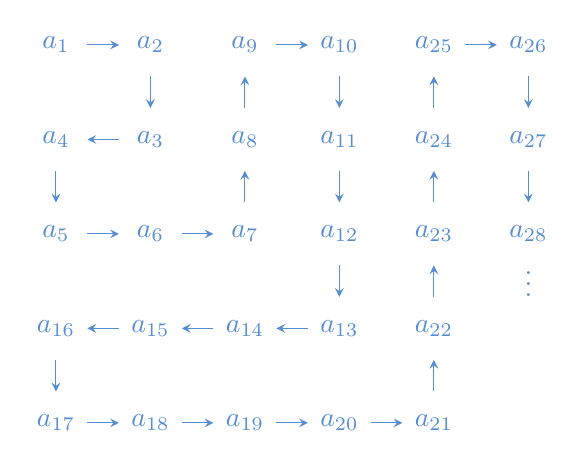
\begin{tikzpicture}[cackithi, scale=0.8]
			\draw (0,4) node {$a_1$};
			\draw (1.5,4) node {$a_2$};
			\draw (1.5,2.5) node {$a_3$};
			\draw (0,2.5) node {$a_4$};
			\draw (0,1) node {$a_5$};
			\draw (1.5,1) node {$a_6$};
			\draw (3,1) node {$a_7$};
			\draw (3,2.5) node {$a_8$};
			\draw (3,4) node {$a_9$};
			\draw (4.5,4) node {$a_{10}$};
			\draw (4.5,2.5) node {$a_{11}$};
			\draw (4.5,1) node {$a_{12}$};
			\draw (4.5,-0.5) node {$a_{13}$};
			\draw (3,-0.5) node {$a_{14}$};
			\draw (1.5,-0.5) node {$a_{15}$};
			\draw (0,-0.5) node {$a_{16}$};
			\draw (0,-2) node {$a_{17}$};
			\draw (1.5,-2) node {$a_{18}$};
			\draw (3,-2) node {$a_{19}$};
			\draw (4.5,-2) node {$a_{20}$};
			\draw (6,-2) node {$a_{21}$};
			\draw (6,-0.5) node {$a_{22}$};
			\draw (6,1) node {$a_{23}$};
			\draw (6,2.5) node {$a_{24}$};
			\draw (6,4) node {$a_{25}$};
			\draw (7.5,4) node {$a_{26}$};
			\draw (7.5,2.5) node {$a_{27}$};
			\draw (7.5,1) node {$a_{28}$};
			\draw [-stealth] (.5,4) -- (1,4);
			\draw [-stealth] (1.5,3.5) -- (1.5,3);
			\draw [-stealth] (1,2.5) -- (0.5,2.5);
			\draw [-stealth] (0,2) -- (0,1.5);
			\draw [-stealth] (0.5,1) -- (1,1);
			\draw [-stealth] (2,1) -- (2.5,1);
			\draw [-stealth] (3,1.5) -- (3,2);
			\draw [-stealth] (3,3) -- (3,3.5);
			\draw [-stealth] (3.5,4) -- (4,4);
			\draw [-stealth] (4.5,3.5) -- (4.5,3);
			\draw [-stealth] (4.5,2) -- (4.5,1.5);
			\draw [-stealth] (4.5,0.5) -- (4.5,0);
			\draw [-stealth] (4,-0.5) -- (3.5,-0.5);
			\draw [-stealth] (2.5,-0.5) -- (2,-0.5);
			\draw [-stealth] (1,-0.5) -- (0.5,-0.5);
			\draw [-stealth] (0,-1) -- (0,-1.5);
			\draw [-stealth] (0.5,-2) -- (1,-2);
			\draw [-stealth] (2,-2) -- (2.5,-2);
			\draw [-stealth] (3.5,-2) -- (4,-2);
			\draw [-stealth] (5,-2) -- (5.5,-2);
			\draw [-stealth] (6,-1.5) -- (6,-1);
			\draw [-stealth] (6,0) -- (6,0.5);
			\draw [-stealth] (6,1.5) -- (6,2);
			\draw [-stealth] (6,3) -- (6,3.5);
			\draw [-stealth] (6.5,4) -- (7,4);
			\draw [-stealth] (7.5,3.5) -- (7.5,3);
			\draw [-stealth] (7.5,2) -- (7.5,1.5);
			\draw (7.5, 0.33) node {$\vdots$};
		\end{tikzpicture}
		\vspace*{-5pt}
	\end{figure}
	Với mỗi $m \ge 1$, biểu diễn thập phân của số thực $z_m$ được cho bằng cách viết chữ số $0$ trước dấu phẩy và sau dấu phẩy là các chữ số của dòng thứ $m$ (tính từ trên xuống) theo thứ tự từ trái sang phải. Tương tự, với mọi $n \ge 1$, số thực $s_n$ được thiết lập với các chữ số của cột thứ $n$ (tính từ bên trái sang) theo thứ tự từ trên xuống dưới. Chẳng hạn $z_3 = 0, a_5a_6a_7a_{12}a_{23}a_{28}\ldots$ và $s_2 = 0,a_2a_3a_6a_{15}a_{18}a_{35}\ldots$. Chứng minh rằng:
	\vskip 0.1cm
	$(a)$ Nếu $\alpha$ là số hữu tỷ, thì tất cả các số $z_m$ và $s_n$ đều hữu tỷ.
	\vskip 0.1cm
	$(b)$ Điều ngược lại của khẳng định $(a)$ là sai.
	\vskip 0.1cm
	\textbf{\color{cackithi}Vòng $\pmb{2.}$}
	\vskip 0.1cm
	\textbf{\color{cackithi}Câu $\pmb{1}$}: Tìm ước chung lớn nhất của tất cả các số có dạng $p^6 - 7p^2 +6$ với $p$ chạy trên tập tất cả các số nguyên tố và $p \ge 11$.
	\vskip 0.1cm
	\textbf{\color{cackithi}Câu $\pmb{2}$}: Trên một hòn đảo địa hình đồi núi có $2023$ điểm quan sát. Từ mỗi điểm quan sát có thể nhìn thấy ít nhất $42$ điểm quan sát khác. Với hai điểm quan sát bất kỳ $X$ và $Y$, luôn tồn tại một số nguyên dương $n$ và các điểm quan sát $A_1,  A_2, \ldots, A_{n+1}$ sao cho $A_1 = X$, $A_{n+1} = Y$ và mỗi cặp điểm liền kề $A_i$ với $A_{i+1}$ có thể quan sát được lẫn nhau với $i = 1, 2, \ldots, n$. Số $n$ nhỏ nhất như vậy được gọi là khoảng cách quan sát (Sichtabstand). 
	\vskip 0.1cm
	Xác định khoảng cách quan sát lớn nhất có thể có giữa hai cặp điểm quan sát thỏa mãn những điều kiện ở trên.
	\vskip 0.1cm
	\textbf{\color{cackithi}Câu $\pmb{3}$}: Cho tam giác $AB$C với tâm đường tròn nội tiếp $I$. Gọi trung điểm của các cạnh $AC$ và $BC$ lần lượt là $M_b$ và $M_a$. Gọi giao điểm của đường thẳng $M_bI$ với đường thẳng $BC$ là $B'$ và giao điểm của đường thẳng $M_aI$ với đường thẳng $AC$ là $A'$. Biết rằng hai tam giác $ABC$ và $A'B'C$ có cùng diện tích. 
	\vskip 0.1cm
	Tìm giá trị lớn nhất có thể của góc $ACB$.
	\vskip 0.1cm
	\textbf{\color{cackithi}Câu $\pmb{4}$}: Cho một đa diện đều $2n$ cạnh. Từ các đoạn thẳng nối các đỉnh của đa diện (cạnh biên hoặc đường chéo) ta tô $n$ cạnh màu đỏ sao cho:
	\vskip 0.1cm
	$1.$ Các điểm cuối của các cạnh màu đỏ chính là $2n$ đỉnh của đa diện.
	\vskip 0.1cm
	$2.$  Không có $2$ cạnh màu đỏ nào có độ dài bằng nhau.
	\vskip 0.1cm
	Tìm tất cả các số tự nhiên $n \ge 2$ thỏa mãn yêu cầu đã cho.
\end{multicols}
\newpage
\begingroup
\AddToShipoutPicture*{\put(150,695){\includegraphics[scale=1]{../tieude1.pdf}}}
\centering
\endgroup
\vspace*{10pt}

\begin{multicols}{2}
	Trong phần đầu chuyên mục, chúng tôi sẽ trình bày với các bạn lời giải của các bài toán trong kỳ thi Olympic toán học trẻ của Thổ Nhĩ Kỳ, đăng trong số báo $5/2023$. 
	\begin{figure}[H]
		\vspace*{-5pt}
		\centering
		\captionsetup{labelformat= empty, justification=centering}
		\includegraphics[width= 1\linewidth]{gocolympic}
		%		\caption{\small\textit{\color{}}}
		\vspace*{-10pt}
	\end{figure}
	{\bf\color{cackithi} OC$\pmb{40.}$} Cho $x, y, z$ là các số thực dương với $x\le 1.$ Chứng minh rằng
	\begin{align*}
		xy+y+2z \geq 4 \sqrt{xyz}.
	\end{align*}
	\textit{Lời giải.} Trong bài này có thể dùng giả thiết $x\le 1$ theo các cách khác nhau dẫn đến những lời giải khác nhau.
	\vskip 0.1cm
	\textit{Lời giải} $1$: từ $x\le 1$ ta có $z \ge zx.$ Kết hợp với bất đẳng thức Cauchy, ta thu được điều cần chứng minh
	\begin{align*}
		xy+y+2z &\ge  xy \!+\!y \!+\! z \!+\! zx = (x\!+\!1)(y\!+\!z) \\
		&\ge 2\sqrt{x}2\sqrt{yz}= 4 \sqrt{xyz}.
	\end{align*}
	\textit{Lời giải} $2$: theo bất đẳng thức Cauchy, ta có $ xy+y+2z=(x+1)y+ 2z \ge 2\sqrt{(x+1)y2z}.$ Từ giả thiết $x\le 1$ ta có $x+1\ge 2x,$ như vậy ta có điều cần chứng minh
	\begin{align*}
		xy+y+2z &\ge 2\sqrt{(x+1)y2z}\\
		&\ge 2\sqrt{2xy2z}= 4\sqrt{xyz}.
	\end{align*} 
	
	{\bf\color{cackithi} OC$\pmb{41.}$} Trong một trường có $101$ học sinh, mỗi học sinh có ít nhất một người bạn thân trong số các học sinh khác trong trường. Chứng minh rằng với mọi số nguyên $n, 1<n<101,$ ta có thể chọn một nhóm $n$ học sinh trong trường này sao cho mỗi học sinh được chọn có ít nhất một bạn thân trong số các học sinh khác được chọn. (Biết rằng nếu  $A$ là bạn thân của $B$ thì $B$ cũng là bạn thân của $A$).
	\vskip 0.1cm
	\textit{Lời giải.}
	Với $n=2,$ kết luận đúng vì ta chỉ cần chọn ra $1$ học sinh cùng với $1$ bạn thân của người đó.
	\vskip 0.1cm
	Nếu ta gọi $d_i$ là số bạn thân mà học sinh thứ $i$ có thì tổng $s=\sum_{i=1}^{101} d_i$ phải là số chẵn vì mỗi cặp bạn thân được tính $2$ lần trong tổng. Độc giả nào biết về lý thuyết đồ thị sẽ nhận ra ngay đây là một kết quả quen thuộc, thường được gọi là Bổ đề bắt tay. Như vậy không thể xảy ra trường hợp mỗi học sinh chỉ có đúng $1$ bạn thân vì khi đó $s=101,$ là số lẻ. Do đó, ta có thể chọn ra một bạn $A$ có ít nhất $2$ bạn thân. Nhóm gồm bạn $A$ và $2$ bạn thân của $A$ thỏa mãn điều kiện đầu bài, tức là kết luận đúng với $n=3$.
	\vskip 0.1cm
	Ta sẽ chứng minh rằng từ nhóm $G$ bất kỳ gồm $n<100$ học sinh thỏa mãn đầu bài, ta luôn có thể thêm vào $2$ học sinh nữa để nhận được nhóm cũng thỏa mãn đầu bài. Thật vậy, xét hai học sinh $A, B$ không thuộc $G.$ Nếu $A$ hoặc $B$ có một bạn thân không nằm trong $G$ thì ta có $1$ cặp bạn thân không thuộc $G.$ Bổ sung cặp bạn thân này vào $G,$ ta được nhóm mới vẫn thỏa mãn đầu bài. Trường hợp còn lại, cả $A$ và $B$ đều phải có bạn thân trong $G,$ lúc này nhóm $G\cup \{A, B\}$ hiển nhiên thỏa mãn đầu bài.
	\vskip 0.1cm
	Như vậy, xuất phát với nhóm gồm $2$ hoặc $3$ học sinh thỏa mãn đầu bài ta có thể xây dựng được nhóm $n$ học sinh thỏa mãn đầu bài với mọi $1<n<101.$    
	\vskip 0.1cm
	{\bf\color{cackithi} OC$\pmb{42.}$} Cho $m, n, a, k$ là các số nguyên dương và $k>1$ sao cho đẳng thức sau thỏa mãn
	\begin{align*}
		5^m+63n+49=a^k.
	\end{align*}
	Tìm giá trị nhỏ nhất của $k$.
	\vskip 0.1cm
	\textit{Lời giải.} Ta sẽ chứng minh trường hợp $k=2, 3, 4$ không xảy ra.
	\vskip 0.1cm
	Giả sử $k=2,$ xét đẳng thức $5^m+63n+49=a^k$ modulo $7$ ta có 
	\begin{align*}
		5^m \equiv a^2 \equiv 0,1,2,4 \pmod{7}.
	\end{align*}
	Do $5^6\equiv 1 \pmod{7},$  ta nhận được $m \equiv 0,2,4 \pmod{6}.$ 
	\vskip 0.1cm
	Như vậy $m$ là số chẵn. Tiếp tục xét modulo $3$, ta có
	\begin{align*}
		5^m+63n+49 \equiv (-1)^{m}+1  \equiv 2 \pmod{3}.
	\end{align*}
	Tuy nhiên điều này dẫn đến $a^2\equiv 2 \pmod{3},$ mâu thuẫn.  
	\vskip 0.1cm
	Giả sử $k=3,$ xét modulo $7$, ta có
	\begin{align*}
		5^m \equiv a^3 \equiv 0,1,6 \pmod{7}.
	\end{align*}
	Từ đó suy ra ra $m \equiv 0,3 \pmod{6},$ tức là $m=3l.$
	\vskip 0.1cm
	Tiếp tục xét modulo $9$, ta có 
	\begin{align*}
		5^m+63n+49 &\equiv (5)^{3l}+4  \equiv (-1)^l +4\\
		&\equiv 3, 5 \pmod{9}.
	\end{align*}
	Tuy nhiên điều này dẫn đến mâu thuẫn vì $a^3\equiv 0, 1, 8 \pmod{9}.$
	\vskip 0.1cm
	Do trường hợp $k=2$ không xảy ra nên $k=4$ cũng không xảy ra vì ta có thể viết $5^m+63n+49=a^4=(a^2)^2.$
	\vskip 0.1cm
	Trường hợp $k=5,$ ta tìm được bộ $m=1, n=3, a=3$ thỏa mãn đẳng thức. Như vậy giá trị nhỏ nhất có thể của $k$ là $5$.
	\vskip 0.1cm
	Trong phần cuối của chuyên mục kỳ này, chúng tôi sẽ giới thiệu với bạn đọc ba bài toán trong Kỳ thi toán Durer lần thứ XVI được tổ chức tại Hungary. Đây là kỳ thi toán đồng đội mang tên Albrecht Durer, một nghệ sĩ, nhà tư tưởng nổi tiếng thời kỳ Phục hưng. Các bài toán sau phù hợp với trình độ học sinh lớp $7-9$.
	\vskip 0.1cm
	{\bf\color{cackithi} OC$\pmb{49.}$} Cho $ABC$ là tam giác cân. Cạnh đáy $BC$ dài $1$ cm, cạnh $AB$ và $AC$ dài $2$ cm. Gọi $F$ là trung điểm của $AB$ và $G$ là trung điểm của $AC.$ Gọi $(k)$ là đường tròn tiếp xúc với $AB$ và $AC$, tương ứng tại $F$ và $G$. Chứng minh rằng giao điểm của $CF$ và $BG$ thuộc đường tròn $(k).$
	\vskip 0.1cm
	{\bf\color{cackithi} OC$\pmb{50.}$} Khi Andris bước vào phòng, có các số $3$ và $24$ trên bảng. Trong một bước, nếu đã có các số (không nhất thiết phải khác nhau) $k$ và $n$ trên bảng, thì
	Andris có thể viết thêm số $kn + k + n$ lên bảng. 
	\vskip 0.1cm
	$(a)$ Liệu Andris có thể viết số  $9999999$ lên bảng sau một số bước?
	\vskip 0.1cm
	$(b)$ Cùng câu hỏi như phần $(a)$ cho số $99999999$?
	\vskip 0.1cm
	$(c)$ Cùng câu hỏi như phần $(a)$ cho số $48999999$?
	\vskip 0.1cm
	{\bf\color{cackithi} OC$\pmb{51.}$} Có một trò chơi với một bảng ô vuông cỡ $3 \times 3$. Trong mỗi bước, người chơi lần lượt điền một trong các số $1$, $2$ hoặc $3$ vào một ô trống sao cho không có hai số giống nhau trong cùng một hàng hoặc trong cùng một cột. Nếu tất cả $9$ ô của bảng đều được điền số, người chơi đầu tiên thắng nhưng nếu trước đó có một thời điểm không thể điền số được nữa thì người chơi thứ hai thắng.
	\vskip 0.1cm
	Hỏi có cách nào để luôn chiến thắng nếu bạn được phép tùy chọn đi trước hoặc đi sau?
\end{multicols}
	\newpage

	\setcounter{figure}{0}
	\thispagestyle{doisongtoanhocnone}
\pagestyle{doisongtoanhoc}
\everymath{\color{doisongtoanhoc}}
\graphicspath{{../doisongtoanhoc/pic/}}
\blfootnote{$^1$\color{doisongtoanhoc}Viện Toán học.}
\begingroup
\AddToShipoutPicture*{\put(0,616){\includegraphics[width=19.3cm]{../bannerdoisong}}}
\AddToShipoutPicture*{\put(64,500){\includegraphics[scale=0.95]{../tieude.pdf}}}\centering
\endgroup

\vspace*{210pt}


\begin{multicols}{2}	
	Từ ngày $08/08/2023$ đến ngày $12/08/2023$, tại Trường Đại học Sư phạm -- Đại học Đà Nẵng, Hội Toán học Việt Nam đã chủ trì và phối hợp với Viện nghiên cứu cao cấp về Toán, Trường Đại học Sư phạm -- Đại học Đà Nẵng, Trường Đại học Khoa học Tự nhiên -- Đại học Quốc gia Hà Nội, Viện Toán học -- Viện Hàn lâm Khoa học và Công nghệ Việt Nam tổ chức Hội nghị Toán học toàn quốc lần thứ X.
	\vskip 0.1cm
	Hội nghị Toán học toàn quốc là hoạt động khoa học lớn nhất của cộng đồng Toán học Việt Nam, được tổ chức $5$ năm một lần. Hội nghị là diễn đàn để các nhà nghiên cứu, ứng dụng và giáo dục toán học trên cả nước trình bày những thành tựu nghiên cứu của mình trong vòng $5$ năm gần đây. Đây cũng là dịp để cộng đồng Toán học Việt Nam, cả trong và ngoài nước, tham gia trao đổi và đóng góp ý kiến về những vấn đề thời sự, cấp thiết đối với sự phát triển Toán học của nước nhà. Tham dự Hội nghị năm nay có hơn $900$ đại biểu đến từ các viện nghiên cứu, học viện, trường đại học và trường trung học phổ thông trên mọi miền đất nước, trong đó có $3$ đại biểu nước ngoài và $90$ nhà toán học Việt Nam đang làm việc ở nước ngoài. Hai nội dung chính của Hội nghị Toán học toàn quốc năm nay là Hội nghị khoa học và Đại hội Đại biểu Hội Toán học Việt Nam lần thứ IX.
	\begin{figure}[H]
		\vspace*{-5pt}
		\centering
		\captionsetup{labelformat= empty, justification=centering}
		\includegraphics[width= 1\linewidth]{2}
		\caption{\small\textit{\color{doisongtoanhoc}GS. TSKH. Vũ hoàng Linh Chủ tịch Hội Toán học Việt Nam nhiệm kỳ $2023-2028$.}}
		\vspace*{-10pt}
	\end{figure}
	Phần Hội nghị khoa học đã diễn ra với $7$ phiên toàn thể và $224$ phiên báo cáo thuộc $10$ tiểu ban: Đại số -- Lý thuyết số, Hình học -- Tôpô, Giải tích, Phương trình vi phân và Hệ động lực, Toán rời rạc và Cơ sở Toán học của Tin học, Tối ưu và Lý thuyết Điều khiển, Xác suất -- Thống kê -- Khoa học dữ liệu, Giải tích số và Ứng dụng Toán học, Giảng dạy và Lịch sử Toán học, Phương trình Đạo hàm riêng. Ban tổ chức đã mời $7$ nhà toán học đọc báo cáo mời tại các phiên toàn thể:
	\vskip 0.1cm
	$1.$ Đinh Tiến Cường (National University of Singapore): \textit{Dynamics of complex Hénon maps};
	\vskip 0.1cm
	$2.$ Đinh Dũng (Đại học Quốc gia Hà Nội): \textit{Sparsity in uncertainty qualification for PDEs with Gaussian random field inputs};
	\vskip 0.1cm
	$3.$ Nguyễn Văn Hoàng (Trường Đại học FPT): \textit{Stability estimates for the sharp Sobolev type inequalities};
	\vskip 0.1cm
	$4.$ Đoàn Thái Sơn (Viện Toán học -- Viện Hàn lâm Khoa học và Công nghệ Việt Nam): \textit{Random dynamical systems};
	\vskip 0.1cm
	$5.$ Phạm Tiến Sơn (Trường Đại học Đà Lạt): \textit{Polynomial optimization from the viewpoint of singularity theory};
	\vskip 0.1cm
	$6.$ Nguyễn Duy Tân (Đại học Bách khoa Hà Nội): \textit{On the Massey vanishing conjecture in Galois cohomology of fields};
	\vskip 0.1cm
	$7.$ Vũ Hà Văn (Yale University, Mỹ): \textit{Random matrices and data recovery}.
	\begin{figure}[H]
		\vspace*{-5pt}
		\centering
		\captionsetup{labelformat= empty, justification=centering}
		\includegraphics[width= 1\linewidth]{3}
		\caption{\small\textit{\color{doisongtoanhoc}PGS. TS. Đoàn Trung Cường Phó Chủ tịch kiêm Tổng Thư ký Hội Toán học Việt Nam nhiệm kỳ $2023-2028$.}}
		\vspace*{-10pt}
	\end{figure}
	Đã có $70$ báo cáo mời tiểu ban và $413$ báo cáo ngắn được trình bày tại các phiên báo cáo tiểu ban. Các báo cáo khoa học được trình bày có chủ đề đa dạng, giới thiệu những hướng nghiên cứu thời sự và các thành tựu nghiên cứu gần đây của các nhà toán học Việt Nam. Có nhiều báo cáo trong số đó là của các nhà toán học trẻ có thành tích nghiên cứu xuất sắc. Đặc biệt, với $110$ báo cáo được trình bày bởi các nhà toán học nữ, đây là kỳ hội nghị có số lượng đại biểu nữ trình bày báo cáo cao nhất từ trước tới nay.
	\vskip 0.1cm
	Trong chương trình Hội nghị, Đại hội Đại biểu Hội Toán học Việt Nam lần thứ IX đã được tổ chức vào ngày $10/08/2023$. Các đại biểu đã bầu ra Ban chấp hành Hội Toán học Việt Nam khóa IX (nhiệm kỳ $2023-2028$), bầu trực tiếp Chủ tịch và Tổng thư ký của Hội. Ban Chấp hành mới đã họp ngay trong chiều ngày $10/08/2023$ và quyết định phân công như sau.
	\vskip 0.1cm
	$1.$ GS. TSKH. Vũ Hoàng Linh (Trường Đại học Khoa học Tự nhiên -- Đại học Quốc gia Hà Nội): \textit{Chủ tịch}.
	\vskip 0.1cm
	$2.$ PGS. TS. Đoàn Trung Cường (Viện Toán học – Viện Hàn lâm Khoa học và Công nghệ Việt Nam): \textit{Phó Chủ tịch kiêm Tổng thư ký}.
	\vskip 0.1cm
	$3.$	GS. TS. Lâm Quốc Anh (Trường Đại học Cần Thơ): \textit{Phó Chủ tịch}.
	\vskip 0.1cm
	$4.$	PGS. TS. Đinh Thanh Đức (Hội Toán học Bình Định): \textit{Phó Chủ tịch}.
	\vskip 0.1cm
	$5.$	GS. TS. Lê Thị Thanh Nhàn (Bộ Giáo dục và Đào tạo): \textit{Phó Chủ tịch}.
	\vskip 0.1cm
	$6.$	GS. TSKH. Đỗ Đức Thái (Trường Đại học Sư phạm Hà Nội): \textit{Phó Chủ tịch}.
	\vskip 0.1cm
	$7.$	PGS. TS. Mai Hoàng Biên (Trường Đại học Khoa học Tự nhiên -- Đại học Quốc gia Thành phố Hồ Chí Minh): \textit{Ủy viên}.
	\vskip 0.1cm
	$8.$	TS. Trần Nam Dũng (Trường Phổ thông Năng khiếu -- Đại học Quốc gia Thành phố Hồ Chí Minh): \textit{Ủy viên}.
	$9.$	PGS. TSKH. Phan Thị Hà Dương (Viện Toán học -- Viện Hàn lâm Khoa học và Công nghệ Việt Nam): \textit{Ủy viên}.
	\vskip 0.1cm
	$10.$	PGS. TS. Lê Văn Hiện (Trường Đại học Sư phạm Hà Nội): \textit{Ủy viên}.
	\end{multicols}
	\begin{figure}[H]
		\vspace*{5pt}
		\centering
		\captionsetup{labelformat= empty, justification=centering}
		\includegraphics[width= 1\linewidth]{1}
		\caption{\small\textit{\color{doisongtoanhoc}Các thành viên Ban Chấp hành và Ban kiểm tra Hội Toán học Việt Nam nhiệm kỳ $2023 - 2028$.}}
		\vspace*{-10pt}
	\end{figure}
	\begin{multicols}{2}
	$11.$	PGS. TSKH. Nguyễn Thiệu Huy (Đại học Bách khoa Hà Nội): \textit{Ủy viên}.
	\vskip 0.1cm
	$12.$	TS. Nguyễn Thị Lê Hương (Viện nghiên cứu cao cấp về Toán): \textit{Ủy viên}.
	\vskip 0.1cm
	$13.$	PGS. TS. Nguyễn Thị Hồng Loan (Trường Đại học Vinh): \textit{Ủy viên}.
	\vskip 0.1cm
	$14.$	PGS. TS. Phạm Quý Mười (Trường Đại học Sư phạm -- Đại học Đà Nẵng): \textit{Ủy viên}.
	\vskip 0.1cm
	$15.$	PGS. TS. Trần Kiêm Minh (Trường Đại học Sư phạm -- Đại học Huế): \textit{Ủy viên}.
	\vskip 0.1cm
	$16.$	PGS. TS. Phạm Hoàng Quân (Trường Đại học Sài Gòn): \textit{Ủy viên}.
	\vskip 0.1cm
	$17.$	PGS. TSKH. Đoàn Thái Sơn (Viện Toán học -- Viện Hàn lâm Khoa học và Công nghệ Việt Nam): \textit{Ủy viên}.
	\vskip 0.1cm
	$18.$	PGS. TS. Phó Đức Tài (Trường Đại học Khoa học Tự nhiên -- Đại học Quốc gia Hà Nội): \textit{Ủy viên}.
	\vskip 0.1cm
	$19.$	GS. TS. Lê Anh Vinh (Bộ Giáo dục và Đào tạo): \textit{Ủy viên}. 
\end{multicols}

	\newpage

	\setcounter{figure}{0}
	 \thispagestyle{gocconone}
\pagestyle{gocco}
\everymath{\color{gocco}}
\graphicspath{{../gocco/pic/}}
\blfootnote{$^1${\color[named]{gocco}Trung tâm Ứng dụng Công nghệ Vũ trụ Tp. Hồ Chí Minh.}}
\begingroup
\AddToShipoutPicture*{\put(0,616){\includegraphics[width=19.3cm]{../bannergocco}}}
\AddToShipoutPicture*{\put(120,525){\includegraphics[scale=1]{../tieude2.pdf}}} 
\centering
\endgroup

\vspace*{185pt}
\begin{multicols}{2}	
	Đối với các tình huống trên bàn cờ, ta thường đánh giá tình hình dựa vào $2$ yếu tố: \textit{Quân} (tương quan lực lượng của đôi bên) và \textit{Thế} (vị trí, sự liên kết giữa các quân). Nhìn chung, những yếu tố này bù đắp, hỗ trợ những khiếm khuyết, ưu -- nhược điểm của nhau. Tuy nhiên, nhiều nhà nghiên cứu lý luận Cờ Tướng đã đồng ý thống nhất rằng, yếu tố \textit{Thế} ảnh hưởng nhiều hơn đến kết quả của cuộc cờ. Trong diễn biến mỗi ván đấu, nếu như những nước đi, các biến hóa của Khai cuộc thường mang nặng tính lý thuyết, đa phần dựa vào những nước đi đã được nghiên cứu theo sách vở và phần mềm, thì những giai đoạn tiếp theo phụ thuộc nhiều vào trình độ cũng như khả năng tính toán của đôi bên. Muốn có được thế tốt trong Trung, Tàn cuộc để hướng tới một kết quả có lợi thì vấn đề điều chuyển quân, hay còn được gọi là \textit{Điều động lực lượng} là một yêu cầu vô cùng quan trọng.
	\vskip 0.1cm
	\textit{Điều động lực lượng} được xem là thời điểm chuyển đổi trạng thái giữa các tình  huống, đó cũng có thể được coi là giai đoạn bước ngoặt, quyết định kết quả sau cùng của mỗi ván đấu. Vì vậy, đòi hỏi các kỳ thủ cần phải nắm rõ đâu là vị trí mấu chốt của cuộc cờ, đồng thời cần có một kế hoạch chi tiết, cụ thể mới có thể đưa những quân lực ở vào những vị trí thuận lợi nhất. 
	\vskip 0.1cm
	Để cụ thể hơn về chủ đề \textit{Điều động lực lượng}, tác giả sẽ gửi tới bạn đọc Pi vài ví dụ tiêu biểu có thể áp dụng vào những tình huống trong thực chiến.
	\begin{figure}[H]
		\vspace*{-5pt}
		\centering
		\captionsetup{labelformat= empty, justification=centering}
		\includegraphics[width= 0.4\textwidth]{1}
		\caption{\small\textit{\color{gocco}Hình $1$.}}
		\vspace*{-10pt}
	\end{figure}
	$1.$ Hình $1$, Quân lực tấn công của đôi bên hoàn toàn tương đồng, Đen đang hơn $1$ Sỹ. Tuy nhiên hệ thống Mã và $2$ Sỹ của Đen đang bị giam chặt bởi Pháo đỏ, Đỏ được quyền đi trước và vận dụng triệt để nghệ thuật Điều động lực lượng để giành chiến thắng như sau:
	\vskip 0.1cm
	$\pmb{1)}$ M$6.7$ P$2-3$\quad  $\pmb{2)}$ S$5.4$ Tg$6.1$\quad $\pmb{3)}$ P$8/8$ Tg$6/1$$(*)$ \quad$\pmb{4)}$ P$8-4$ P$3-6$\quad  $\pmb{5)}$ S$4/5$ P$6-3$$(**)$ \quad$\pmb{6)}$ M$7/5$ M$4.5$\quad $\pmb{7)}$ M$5.3$ M$5/7$\quad  $\pmb{8)}$ M$3/4$ S$5.6$\quad $\pmb{9)}$ M$4.6$ S$6/5$\quad $\pmb{10)}$ M$6.7$$(***)$ (Đen mất Pháo, chắc chắn thua cuộc)
	\vskip 0.1cm
	\textit{$(*)$: Nhận ra điểm yếu, Đỏ lập tức lao Mã tới bắt Mã Đen, buộc Đen phải bình Pháo cản khiến cho cả đội hình của Đen kẹt cứng, chỉ có thể di chuyển Tướng. Đỏ tiếp tục giương Sỹ làm ngòi rồi thoái Pháo về đáy dọa sát.
	\vskip 0.1cm
	$(**)$: Đỏ liên tục bình Pháo rồi thoái Sỹ uy hiếp. Để tránh mất quân, Đen lại phải bình Pháo về chỗ cũ. Như vậy sau vài nước điều quân cực kỳ mẫu mực của Đỏ, Đội hình của Đen vẫn không có gì thay đổi.
	\vskip 0.1cm
	$(***)$: Sau khi đem Pháo về vị trí chiến lược, Đỏ tiếp tục có những nước điều động Mã uy hiếp đầy uy lực. Đen đã rất cố gắng chống đỡ nhưng cuối cùng đành chấp nhận thất bại.}
	\begin{figure}[H]
		\vspace*{-5pt}
		\centering
		\captionsetup{labelformat= empty, justification=centering}
		\includegraphics[width= 0.4\textwidth]{2}
		\caption{\small\textit{\color{gocco}Hình $2$.}}
		\vspace*{-10pt}
	\end{figure}
	$2.$ Hình $2$, thoạt nhìn có thể thấy Đen còn chiến Xe và Chốt áp sát rất mạnh, Đỏ chỉ Pháo, Mã, Chốt đang ở những vị trí không thuận lợi cho lắm. Nếu sắp tới Đỏ không có những động thái rõ ràng, Đen sẽ nhanh chóng giành thắng lợi. Tuy nhiên, Đỏ được quyền đi trước và liên tục có những nước đi chính xác như sau:
	\vskip 0.1cm
	$\pmb{1)}$	M$5/3$ Tg$6/1$\quad $\pmb{2)}$ P$5-1$ M$5.7$$(*)$\quad  $\pmb{3)}$ P$1.1$ Tg$6/1$\quad $\pmb{4)}$ M$3.4$  M$7.5$$(**)$\quad  $\pmb{5)}$ C$2-3$ Tg$6.1$\quad $\pmb{6)}$ M$4.2$ M$5/7$\quad $\pmb{7)}$ P$1-3$ X$4/1$$(***)$\quad $\pmb{8)}$ M$2/3$ Tg$6.1$\quad $\pmb{9)}$ P$3-1$ X$4-7$\quad $\pmb{10)}$ M$3.2$ X$7.1$\quad $\pmb{11)}$ P$1-3$$(****)$ $(1-0)$
	\vskip 0.1cm
	\textit{$(*)$: Sau $2$ nước điều chuyển Pháo Mã, Đỏ đưa được những quân chiến tới những điểm trọng yếu, chuẩn bị đi M$3.2$ rồi bình Chốt chiếu bí. Để chừa đường thoát cho Tướng, Đen phải di chuyển Mã ngay lập tức.
	\vskip 0.1cm
	$(**)$: Lợi dụng quân lực của Đen đang ở trạng thái chen chúc, Đỏ tấn Pháo chiếu Tướng kiềm chế rồi sau đó nhảy Mã thẳng vào chân Sỹ. Lúc này, nếu Đen dùng Sỹ ăn Mã hoặc di chuyển Mã, Đỏ sẽ chơi C$2-3$ sát cục ngay lập tức.
	\vskip 0.1cm
	$(***)$: Sau vài nước tấn công dồn dập bằng bộ ba Pháo -- Mã -- Chốt, Đỏ đã ép Đen nhảy Mã vào tử địa, đồng thời lại tiếp tục dọa nước M$3/2$ chiếu tướng bắt chết Xe.
	\vskip 0.1cm
	$(****)$: Mặc dù Đen đã tiêu diệt được Chốt đối phương nhưng vẫn không tài nào thoát được đòn tiền Mã hậu Pháo của Đỏ. Đen mất hết quân, Đỏ thắng cuộc.}
	\begin{figure}[H]
		\vspace*{-5pt}
		\centering
		\captionsetup{labelformat= empty, justification=centering}
		\includegraphics[width= 0.4\textwidth]{3}
		\caption{\small\textit{\color{gocco}Hình $3$.}}
		\vspace*{-10pt}
	\end{figure}
	$3.$ Hình $3$, Trong tình huống thông thường, tàn Xe--Mã đánh xe $2$ Sỹ, (bên Xe--Mã không còn Sỹ, Tượng) thì rất khó giành chiến thắng. Tuy nhiên, với tình huống cụ thể này, Tướng của bên Đen đang bị cheo leo ở hàng $3$, Đỏ đi trước và khai thác một cách triệt để như sau:
	\vskip 0.1cm
	$\pmb{1)}$	M$2/3$ X$5-4$\quad  $\pmb{2)}$ M$3.4$ X$4-6$\quad $\pmb{3)}$ X$4-5$ Tg$5-4$\quad $\pmb{4)}$ X$5-6$ Tg$4-5$\quad $\pmb{5)}$ X$6.1$$(*)$ S$5/6$\quad $\pmb{6)}$ X$6-5$ Tg$5-4$\quad $\pmb{7)}$ Tg$4-5$ X$6-4$\quad $\pmb{8)}$ X$5.2$ Tg$4/1$\quad $\pmb{9)}$ M$4.6$$(**)$ $(1-0)$
	\vskip 0.1cm
	\textit{$(*)$: Nhận thấy điểm yếu Đen, Đỏ điều Mã tới vị trí đẹp, ép Xe Đen rời khỏi vị trí trọng yếu. Và tiếp theo đó là $2$ nước bình xe chiếu Tướng rồi tấn lên bảo vệ Mã, khiến cho Đen rơi vào trạng thái khó đi (Tướng kẹt cứng, Xe phải canh chân Mã)
	\vskip 0.1cm
	$(**)$: Đỏ tiếp tục có thủ đoạn dùng Xe và Tướng chiếm lấy trung lộ, Đen lại phải chạy Xe giữ mặt nhưng lại vướng chân Mã. Đỏ nhẹ nhàng tung đòn chiếu tướng bắt Xe, Đen chắc chắn thất bại.}
	\vskip 0.1cm
	\textit{Chú thích}: C: Chốt, X: Xe, M: Mã, P: Pháo, Tg: Tướng, S: Sĩ, T: Tượng. 
	\vskip 0.1cm
	\textbf{\color{gocco}Câu đố kỳ này:} Đỏ được quyền đi trước, phải khéo léo điều chuyển quân như thế nào để giành lấy thắng lợi trong những hình cờ dưới đây?
	\begin{figure}[H]
		\vspace*{5pt}
		\centering
		\captionsetup{labelformat= empty, justification=centering}
		\includegraphics[width= 0.4\textwidth]{4}
		\caption{\small\textit{\color{gocco}Hình $4$.}}
		\vspace*{-10pt}
	\end{figure}
	\textit{Đáp án tham khảo:} $\pmb{1)}$ M$5.7$ Tg$4/1$\quad $\pmb{2)}$ M$7/8$ Tg$4/1$\quad  $\pmb{3)}$ M$8/7$ X$8.3$\quad $\pmb{4)}$ Tg$5/1$  Tg$4.1$\quad  $\pmb{5)}$ M$7.8$ Tg$4/1$ \quad$\pmb{6)}$ M$8.7$ Tg$4.1$\quad $\pmb{7)}$ M$7/5$ Tg$4/1$\quad $\pmb{8)}$ M$5/7$ Tg$4.1$\quad $\pmb{9)}$ M$7/8$ Tg$4/1$\quad $\pmb{10)}$ M$8/7$ X$8/2$\quad $\pmb{11)}$ M$7/6$ $(1-0)$
	\begin{figure}[H]
		\vspace*{-5pt}
		\centering
		\captionsetup{labelformat= empty, justification=centering}
		\includegraphics[width= 0.4\textwidth]{5}
		\caption{\small\textit{\color{gocco}Hình $5$.}}
		\vspace*{-10pt}
	\end{figure}
	\textit{Đáp án tham khảo:} 
	$\pmb{1)}$ C$5-6$ Tg$4/1$\quad $\pmb{2)}$ T$1/3$ X$9-7$\quad  $\pmb{3)}$ P$3/8$ X$7/1$\quad $\pmb{4)}$ P$4-6$  X$7-4$\quad  $\pmb{5)}$ C$6.1$ Tg$4/1$\quad $\pmb{6)}$ C$6.1$ $(1-0)$
\end{multicols}





	\newpage

%	\thispagestyle{empty}
%	\begingroup 
%	\AddToShipoutPicture*{\put(0,0){\includegraphics[width=19.3cm]{dovui.pdf}}}
%	\centering
%	\vspace*{0cm}
%	\endgroup
%	\newpage	
%	\pagestyle{empty}
\end{document} 

	\setcounter{figure}{0}
\thispagestyle{timhieukhoahocnone}
\pagestyle{timhieukhoahoc}
\everymath{\color{timhieukhoahoc}}
\blfootnote{$^1$\text{\color{timhieukhoahoc}Hà Nội.}}
\graphicspath{{../timhieukhoahoc/pic2/}}
\begingroup
\AddToShipoutPicture*{\put(0,616){\includegraphics[width=19.3cm]{../bannertimhieu}}}
\AddToShipoutPicture*{\put(41,552){\includegraphics[scale=1]{../tieude1.pdf}}}
\centering
\endgroup
\vspace*{155pt}

\begin{multicols}{2}
	Trong số trước của Pi, chúng ta đã tìm hiểu quá trình Pascal khám phá ra nguyên lý mang tên ông về áp suất trong lòng chất lỏng. Bài viết này sẽ trình bày những ứng dụng của nguyên lý trên trong các hiện tượng tự nhiên cũng như các công cụ sử dụng thủy lực đa dạng trong đời sống.
	\vskip 0.1cm
	$\pmb{1.}$ \textbf{\color{timhieukhoahoc}Ứng dụng của bình thông nhau}
	\begin{figure}[H]
		\vspace*{-5pt}
		\centering
		\captionsetup{labelformat= empty, justification=centering}
		\includegraphics[width= 1\linewidth]{1}
		\caption{\small\textit{\color{timhieukhoahoc}Hình $1$. Quy trình hoạt động của tháp nước: $1$. Nước được bơm lên bể trên tháp. $2$. Bể trên tháp có tác dụng như cột nước ở một nhánh của bình thông nhau. $3$. Các vòi nước ở nhà dân đóng vai trò nhánh còn lại.}}
		\vspace*{-5pt}
	\end{figure}
	Một ứng dụng rất thực tế của mô hình bình thông nhau trong đời sống là các tháp nước. Nước được bơm lên và chứa trong các bể cao ở đỉnh tháp. Áp suất do nước trong bể sẽ được truyền theo đường ống và tạo thành áp suất nước khi ta mở các van lấy nước sinh hoạt. Với những tầng nhà càng cao thì áp suất nước sẽ càng giảm đi do chênh lệch độ cao với tháp nước giảm. Các đài phun nước cũng là một ứng dụng khác của bình thông nhau trong thực tiễn đời sống.
	Một hiện tượng tương tự trong tự nhiên là các giếng phun. Ở những vị trí có độ cao nằm dưới mực nước ngầm của một khu vực, khi ta khoan giếng, việc này cũng giống như mở một nhánh mới của bình thông nhau và áp suất nước sẽ khiến nước tự phun lên mặt đất giống như vòi phun vậy. 
	\begin{figure}[H]
		\vspace*{-5pt}
		\centering
		\captionsetup{labelformat= empty, justification=centering}
		\includegraphics[width= 1\linewidth]{2}
		\includegraphics[width= 1\linewidth]{3}
		\caption{\small\textit{\color{timhieukhoahoc}Hình $2$. Giếng phun trong tự nhiên xuất hiện tại các vị trí nằm dưới mực nước ngầm của khu vực.}}
		\vspace*{-5pt}
	\end{figure}
	\begin{figure}[H]
		\vspace*{5pt}
		\centering
		\captionsetup{labelformat= empty, justification=centering}
		\includegraphics[width= 1\linewidth]{4}
		\caption{\small\textit{\color{timhieukhoahoc}Hình $3$. Gióng hàng theo phương ngang sử dụng ống chứa nước. Đây là một phương pháp rẻ và hiệu quả trước khi có sự xuất hiện của các thiết bị sử dụng laser.}}
		\vspace*{-10pt}
	\end{figure}
	Do mực nước ở hai nhánh của bình thông nhau luôn ngang hàng nên trong xây dựng, người ta có thể dùng một ống nhựa trong suốt (hoặc hai hình trụ thủy tinh gắn với hai đầu một ống nối) chứa nước để tiến hành gióng hàng theo phương ngang. Thao tác gióng hàng sẽ cần có hai người. Một người giữ một nhánh ống ở vị trí cố định. Người kia dùng mực nước ở nhánh còn lại để đánh dấu vị trí ngang hàng. Các bạn học sinh cũng có thể thử làm thí nghiệm này trên lớp nhưng cần chú ý không bao giờ để hai đầu ống có chênh lệch độ cao quá lớn, nếu không nước sẽ bị trào ra. 
	\begin{figure}[H]
		\vspace*{-5pt}
		\centering
		\captionsetup{labelformat= empty, justification=centering}
		\includegraphics[width= 1\linewidth]{5}
		\caption{\small\textit{\color{timhieukhoahoc}Hình $4$. Khi đo huyết áp, vị trí đo cần ngang hàng với tim để kết quả đo được chính xác.}}
		\vspace*{-10pt}
	\end{figure}
	Tương tự, khi bác sĩ tiến hành đo huyết áp cho bệnh nhân, để kết quả đo gần với áp suất của máu ở tim nhất, vị trí đo huyết áp cần có độ cao ngang hàng với tim của người được đo. Thật vậy, hệ tuần hoàn của cơ thể cũng giống như một hệ thống bình thông nhau với nhiều nhánh!
	\vskip 0.1cm
	Cơ chế hoạt động trên cũng có thể được sử dụng để chế tạo thiết bị đo áp suất. Nếu ta đổ chất lỏng vào một bình thông nhau dạng chữ U, khi cả hai đầu của mỗi nhánh đều hở và tiếp xúc với không khí thì mực chất lỏng ở hai nhánh sẽ bằng nhau. Nếu một đầu được cho tiếp xúc với một bình chứa khí thì độ chênh lệch mực chất lỏng giữa hai nhánh sẽ cho ta độ chênh lệch về áp suất của khí trong bình chứa với áp suất khí quyển:
	\begin{align*}
		\Delta p = \rho g |\Delta h|
	\end{align*}
	với $\rho$ là mật độ của chất lỏng trong ống. 
	\vskip 0.1cm
	Nếu mực chất lỏng trong nhánh tiếp xúc với bình chứa khí thấp hơn nhánh còn lại thì áp suất trong bình chứa sẽ cao hơn áp suất khí quyển. Ngược lại, nếu mực chất lỏng trong ống này thấp hơn nhánh tiếp xúc với không khí thì áp suất của khối khí sẽ thấp hơn áp suất của khí quyển.
	\vskip 0.1cm
	Tương tự, nếu mỗi nhánh của ống tiếp xúc với một khối khí khác nhau, ta cũng có thể dùng cách này để đo sự chênh lệch áp suất giữa hai khối khí đó giống với trường hợp so sánh với áp suất khí quyển (Hình $5b$). Cách làm này có thể giúp xác định rò rỉ của đường ống dẫn khí bằng cách đo chênh lệch áp suất giữa hai vị trí khác nhau của đường ống.
	\vskip 0.1cm
	Người ta cũng có thể đo giá trị tuyệt đối của áp suất thay cho độ chênh lệch áp suất nếu một nhánh của ống là kín và phần phía trên của mặt chất lỏng là chân không. Trong trường hợp độ cao của cột chất lỏng quá lớn, ta có thể lắp nhiều ống chữ U nối với nhau, phần giữa của chúng được bơm khí nén có tác dụng truyền áp suất giống như với chất lỏng (Hình $5d$). Để tìm giá trị đo của áp suất, ta cần lấy tổng tất cả các độ chênh lệch mực chất lỏng của các ống chữ U.
	\begin{figure}[H]
		\vspace*{5pt}
		\centering
		\captionsetup{labelformat= empty, justification=centering}
		$a)$\includegraphics[height = 0.4\linewidth]{6}
		$b)$\includegraphics[height = 0.4\linewidth]{7}
		
		$c)$\includegraphics[height = 0.4\linewidth]{8}
		$d)$\includegraphics[height = 0.4\linewidth]{9}
		\caption{\small\textit{\color{timhieukhoahoc}Hình $5$. Đo áp suất chất khí bằng ống chữ U. $a)$ Đo chênh lệch áp suất của khối khí so với khí quyển. $b)$ Đo chênh lệch áp suất giữa hai chất khí. $c)$ Ống chữ U đo áp suất trong thực tế. $d)$ Nối các ông chữ U liên tiếp với nhau cho phép đo các áp suất lớn.}}
		\vspace*{-10pt}
	\end{figure}
	Một dạng biến thể khác của ống chữ U được thiết kế với một nhánh có thiết diện lớn hơn nhiều nhánh còn lại (tạo thành một giếng). Khi tiến hành đo, áp suất lớn hơn bao giờ cũng được gắn vào nhánh có giếng. Độ chênh lệch chất lỏng giữa hai nhánh vẫn sẽ giống như với ống chữ U thông thường nhưng chất lỏng bên nhánh giếng sẽ bị dịch chuyển ít hơn nhiều. Người ta có thể tính toán bù trừ lại sự dịch chuyển này để thiết lập thang đo trực tiếp cho nhánh còn lại. Nhánh còn lại cũng có thể được thay bằng một nhánh nghiêng cho độ nhạy tốt hơn và giúp đo các chênh lệch áp suất nhỏ hơn.
	\begin{figure}[H]
		\vspace*{-5pt}
		\centering
		\captionsetup{labelformat= empty, justification=centering}
		$a)$\includegraphics[height = 0.31\linewidth]{10}
		$b)$\includegraphics[height = 0.31\linewidth]{11}
		\caption{\small\textit{\color{timhieukhoahoc}Hình $6$. $a)$ Ống chữ U đo áp suất với một nhánh dạng giếng. $b)$ Một nhánh có dạng giếng, nhánh còn lại là nhánh nghiêng.}}
		\vspace*{-10pt}
	\end{figure}
	\textbf{\color{timhieukhoahoc}Bài tập}
	\vskip 0.1cm
	$1$. Trong hình $6a$, giếng có thiết diện $S_1$, nhánh còn lại có thiết diện $S_2$. Ban đầu hai mực chất lỏng sẽ ngang nhau. Khi có chênh lệch áp suất ứng với chênh lệch độ cao $\Delta h$ giữa hai mực chất lỏng, mực chất lỏng trong nhánh có giếng sẽ đi xuống một đoạn $h_1$ còn mực chất lỏng trong nhánh còn lại sẽ dâng lên một đoạn $h_2$.
	\vskip 0.1cm
	$a)$ Viết phương trình liên hệ $\Delta h,h_1,h_2$.
	\vskip 0.1cm
	$b)$ Viết phương trình liên hệ $h_1,h_2,S_1,S_2$.
	\vskip 0.1cm
	$c)$ Thiết lập biểu thức của $h_2$ theo $\Delta h$ và đề xuất cách tạo thang vạch chia để đọc $\Delta h$ theo mực chất lỏng bên nhánh nhỏ.
	\vskip 0.1cm
	$2.$ Làm tương tự bài $1$ cho trường hợp hình $6b$. Nhánh nghiêng tạo một góc $\alpha$ so với phương nằm ngang.
	\begin{figure}[H]
		\vspace*{-5pt}
		\centering
		\captionsetup{labelformat= empty, justification=centering}
		\includegraphics[width= 0.5\linewidth]{12}
		\caption{\small\textit{\color{timhieukhoahoc}Hình $6$. Di chuyển tàu giữa hai mực nước chênh lệch nhau ở hai phía đập. Trái: tàu đi lên cao. Phải: tàu đi xuống thấp.}}
		\vspace*{-10pt}
	\end{figure}
	Cơ chế của bình thông nhau còn xuất hiện trong các hệ thống vận chuyển tàu thuyền qua các con đập. Người ta tạo một khoảng trung gian giữa hai mực nước với hai cửa chặn. Khi tàu đi vào khoảng này, cả hai cửa đều được đóng. Sau đó người ta mở van ở phía tàu muốn tới. Theo nguyên tắc của bình thông nhau, sau một thời gian, mực nước ở vị trí tàu và phía nó muốn đến sẽ bằng nhau. Chỉ cần mở cửa ở phía này là tàu có thể tiếp tục đi được. Phương pháp trên có thể giúp tàu đi lên cao hoặc xuống thấp cho dù hai phía đập có chênh lệch về độ cao. Trong một số trường hợp, đề tăng hiệu quả sử dụng nước, các hệ thống vận chuyển này được thiết kế ở dạng nhiều tầng. 
	\vskip 0.1cm
	Hệ thống di chuyển tàu thuyền qua đập như trên lần đầu tiên được xây dựng ở Trung Quốc vào cuối thế kỷ $10$ thời nhà Tống. Các công trình tương tự chỉ bắt đầu xuất hiện ở châu Âu vào cuối thế kỷ $14$. Ngày nay, nhiều đập lớn hiện đại như kênh đào Panama sử dụng cách này để giúp tàu thuyền lưu thông qua đập. 
	\vskip 0.1cm
	$\pmb{2.}$ \textbf{\color{timhieukhoahoc}Khuyếch đại lực nhờ hệ thống thủy lực}
	\begin{figure}[H]
		\vspace*{-5pt}
		\centering
		\captionsetup{labelformat= empty, justification=centering}
		\includegraphics[width= 1\linewidth]{13}
		\includegraphics[width= 1\linewidth]{14}
		\caption{\small\textit{\color{timhieukhoahoc}Hình $7$. Cấu tạo của một kích thủy lực. Trên: hai piston ở hai nhánh của bình thông nhau. Dưới: đòn bẩy giúp tăng cường lực ép lên piston nhỏ. Lực ấn của tay được khuyếch đại theo tỉ lệ giữa hai tay đòn.}}
		\vspace*{-10pt}
	\end{figure}
	Việc khuyếch đại lực nhờ thủy lực cũng có nhiều ứng dụng trong đời sống. Một ví dụ thường được nhắc đến là kích thủy lực. Cấu tạo cơ bản của nó gồm hai piston ở hai nhánh của một bình thông nhau. Khi ta tác dụng một lực lên piston của nhánh nhỏ thì lực này được khuyếch đại ở piston của nhánh lớn. Trước đó, lực ấn của tay cũng đã được khuyếch đại một lần thông qua một đòn bẩy với độ khuyếch đại bằng với tỉ lệ tay đòn của vị trí ấn tay và vị trí của piston nhỏ. Hệ thống kích thủy lực dạng này giúp ta nâng lên những vật thể nặng, thậm chí cả các phương tiện như ô tô, tùy theo cấu tạo và khả năng khuyếch đại của kích thủy lực. Một số thiết bị sử dụng nguyên lý này được minh họa trong Hình $8$. Trong một số loại thang máy, hệ thống thủy lực cũng được sử dụng để di chuyển thang máy thay vì sử dụng một bộ ròng rọc.
	\begin{figure}[H]
		\vspace*{-5pt}
		\centering
		\captionsetup{labelformat= empty, justification=centering}
		\includegraphics[height= 0.55\linewidth]{15}
		\includegraphics[height= 0.55\linewidth]{16}
		\includegraphics[height= 0.465\linewidth]{17}
		\includegraphics[height= 0.465\linewidth]{18}
		\caption{\small\textit{\color{timhieukhoahoc}Hình $8$. Một số thiết bị nâng sử dụng thủy lực trong sản xuất và vận chuyển.}}
		\vspace*{-10pt}
	\end{figure}
	Hệ thống nâng thủy lực cũng có thể được dùng ở một số cầu nơi có nhiều tàu thuyền đi lại. Vào những giờ cố định, nhịp cầu sẽ được kéo mở hoặc đẩy lên để các tàu thuyền với chiều cao lớn có thể đi qua bên dưới.
	\begin{figure}[H]
		\vspace*{-5pt}
		\centering
		\captionsetup{labelformat= empty, justification=centering}
		\includegraphics[width= 1\linewidth]{19}
		%		\includegraphics[width= 1\linewidth]{20}
		%		\caption{\small\textit{\color{timhieukhoahoc}Hình $9$. Một số cầu có hệ thống thủy lực để di chuyển nhịp cầu cho tàu thuyền đi qua.}}
		\vspace*{-10pt}
	\end{figure}
	\begin{figure}[H]
		\vspace*{5pt}
		\centering
		\captionsetup{labelformat= empty, justification=centering}
		%		\includegraphics[width= 1\linewidth]{19}
		\includegraphics[width= 1\linewidth]{20}
		\caption{\small\textit{\color{timhieukhoahoc}Hình $9$. Một số cầu có hệ thống thủy lực để di chuyển nhịp cầu cho tàu thuyền đi qua.}}
		\vspace*{-10pt}
	\end{figure}
	Trong trường hợp piston lớn có chuyển động hướng xuống phía dưới, thay vì hệ thống nâng, ta có một hệ thống nén thủy lực. Hệ thống nén dạng này có nhiều ứng dụng trong công nghiệp như giúp nén phẳng các tấm kim loại, nghiền phế liệu, ...
	\begin{figure}[H]
		\vspace*{-5pt}
		\centering
		\captionsetup{labelformat= empty, justification=centering}
		\includegraphics[width= 0.85\linewidth]{21}
		\caption{\small\textit{\color{timhieukhoahoc}Hình $10$. Máy ép thủy lực. Piston lớn sẽ chuyển động theo phương hướng xuống trong các thiết bị này.}}
		\vspace*{-10pt}
	\end{figure}
	Do đặc điểm truyền áp suất theo chất lỏng, hệ thống thủy lực trong công nghiệp không chỉ giúp khuếch đại lực mà còn có tác dụng làm chuyển hướng lực. Ví dụ như trong một máy xúc, cánh tay của nó cần phải gấp ở những khớp nối. Các đường ống dẫn chất lỏng (màu đen trong hình) có thể uốn cùng với chuyển động của cánh tay và cho phép truyền lực theo bất cứ hướng nào mà ta muốn.
	\begin{figure}[H]
		%		\vspace*{5pt}
		\centering
		\captionsetup{labelformat= empty, justification=centering}
		\includegraphics[width= 0.45\linewidth]{22}
		\caption{\small\textit{\color{timhieukhoahoc}Hình $11$. Tay máy xúc được điều khiển bằng thủy lực.}}
		\vspace*{-10pt}
	\end{figure}
	\begin{figure}[H]
		\vspace*{-5pt}
		\centering
		\captionsetup{labelformat= empty, justification=centering}
		\includegraphics[width= 1\linewidth]{23}
		\caption{\small\textit{\color{timhieukhoahoc}Hình $12$. Hệ thống phanh xe sử dụng thủy lực.}}
		\vspace*{-10pt}
	\end{figure}
	Một ví dụ thú vị khác là trong hệ thống phanh xe sử dụng thủy lực (Hình $12$). Khi người lái xe ấn vào chân phanh, cần phanh thực chất có cấu tạo là một đòn bẩy nên lực nhấn vào hệ thống phanh sẽ lớn hơn nhiều lực đạp do tay đòn của nó ngắn hơn (ví dụ $4$ cm so với $20$ cm như trong hình). Lực nhấn này tác động vào một xi lanh có đường kính nhỏ ($0,5$ cm trong hình). Nhờ hệ thống thủy lực, lực tác động lên má phanh lại được khuyếch đại một lần nữa (bạn đọc có thể tự tính xem lực đạp $100N$ ban đầu của người lái xe được khuyếch đại thành lực có độ lớn bao nhiêu tại má phanh). Một điều đáng chú ý khác là hệ thống thủy lực cũng có thể phanh nhiều bánh xe cùng lúc, với mỗi bánh xe ta chỉ cần trang bị thêm một xi lanh nối vào hệ thống thủy lực. Tuy nhiên, như nguyên tắc trong tất cả các hệ thống thủy lực khác, khi ta được lợi về lực thì sẽ thiệt về quãng đường. Vì công do người thực hiện và công tác động lên các bánh xe là như nhau nên với cùng một khoảng cách đạp chân quãng đường di chuyển của xi lanh ở mỗi bánh xe sẽ càng ngắn nếu ta có càng nhiều bánh xe. 
	\vskip 0.1cm
	Với những phương tiện có quán tính lớn, ví dụ xe ủi, người ta có thể lắp đặt thêm hệ thống sử dụng chân không hoặc sử dụng phanh có động cơ thay vì đạp chân một cách thủ công. Trong các máy bay, hệ thống thủy lực không chỉ được dùng cho hệ thống phanh mà còn có nhiều tác dụng khác. Với sự kết hợp các bồn chứa chất lỏng, van định hướng và nhiều piston, người ta có thể điều chỉnh các bộ phận phức tạp của máy bay như cánh, đuôi, bộ phận hạ cánh, ...
	\begin{figure}[H]
		\vspace*{-5pt}
		\centering
		\captionsetup{labelformat= empty, justification=centering}
		\includegraphics[width= 1\linewidth]{24}
		
		\vspace*{4pt}
		\includegraphics[width= 1\linewidth]{25}
		\caption{\small\textit{\color{timhieukhoahoc}Hình $13$. Một số công cụ lao động thủy lực. Trên: cờ lê thủy lực. Dưới: máy cắt thủy lực}}
		\vspace*{-10pt}
	\end{figure}
	Hệ thống thủy lực cũng được sử dụng cho các công cụ cầm tay, ví dụ như cờ lê thủy lực, máy cắt thủy lực, ... 
	\vskip 0.1cm
	$\pmb{3.}$ \textbf{\color{timhieukhoahoc}Đôi nét về lịch sử: Joseph Bramah và William Armstrong}
	\begin{figure}[H]
		\vspace*{-5pt}
		\centering
		\captionsetup{labelformat= empty, justification=centering}
		\includegraphics[width= 1\linewidth]{26}
		\caption{\small\textit{\color{timhieukhoahoc}Joseph Bramah $(1748-1814)$.}}
		\vspace*{-10pt}
	\end{figure}
	Về mặt lịch sử, tuy rằng Pascal đã trình bày lý thuyết về cách khuyếch đại lực sử dụng thủy lực từ thế kỷ $17$, các thiết bị sử dụng nguyên lý này chỉ xuất hiện lần đầu trong thực tiễn vào cuối thế kỷ $18$ với  máy ép thủy lực đầu tiên được Joseph Bramah chế tạo. Sự kiện này đánh dấu một bước tiến quan trọng của cuộc cách mạng công nghiệp ở nước Anh khi đó. Nhiều cỗ máy thủy lực tiếp theo đã được sáng chế phục vụ các công việc khác nhau trong sản xuất. Đến giữa thế kỷ $19$, William Armstrong đã nghiên cứu cách sử dụng thủy lực cho các cần cẩu cỡ lớn phục vụ vận chuyển hàng hóa ở các bến cảng và bắt đầu tiến hành sản xuất chúng hàng loạt với nhà máy có quy mô lên đến $20000$ công nhân. Cây cầu ở thành phố Newcastle cũng được Armstrong xây dựng lại với hệ thống thủy lực cho phép nâng nhịp cầu lên khi các tàu thuyền lớn cần đi qua để vào cảng.
	\vskip 0.1cm
	Dựa trên ý tưởng trước đó của Bramah, Armstrong tiến hành thử nghiệm các hệ thống cung cấp áp lực cho hoạt động của các máy thủy lực. Sau thử nghiệm thất bại với tháp nước do chiều cao cần xây dựng quá lớn, ông sử dụng hệ thống gồm bình chứa lớn với một piston đè lên khối nước bên dưới. Phía trên piston có nhiều quả nặng khối lượng lớn tạo áp suất lên khối nước. Đáy bình được nối với hệ thống đường ống dẫn đến nơi các hệ thống máy móc cần hoạt động, tương tự như mạng điện của chúng ta ngày nay. Những bình chứa của Armstrong còn được gọi là các thiết bị tích tụ thủy lực. Chúng nhanh chóng được phổ biến ở nước Anh cũng như một số nơi khác ở châu Âu. Các mạng áp suất thủy lực này vẫn được duy trì hoạt động cho đến những năm $70$ của thế kỷ $20$. Nhiều thiết bị tích tụ thủy lực hiện đại dạng cải tiến dùng khí nén hoặc lò xo được sử dụng trong nhiều máy móc công nghiệp đa dạng ngày nay.
	\begin{figure}[H]
		\vspace*{-5pt}
		\centering
		\captionsetup{labelformat= empty, justification=centering}
		\includegraphics[width= 1\linewidth]{28}
		\caption{\small\textit{\color{timhieukhoahoc}Cần cẩu thủy lực của Armstrong có thể nâng các khối hàng hóa nặng hàng trăm tấn.}}
		\vspace*{-10pt}
	\end{figure}
	Đặc biệt, Armstrong đã tiên đoán từ thế kỷ $19$ rằng các nhiên liệu như than đá sẽ cần được thay thế bằng các nguồn năng lượng như thủy điện hay năng lượng mặt trời. Ngôi nhà của Armstrong ở Newcastle cũng là ngôi nhà đầu tiên trên thế giới được thắp sáng nhờ thủy điện.
	\begin{figure}[H]
		\vspace*{-5pt}
		\centering
		\captionsetup{labelformat= empty, justification=centering}
		\includegraphics[width= 1\linewidth]{27}
		\caption{\small\textit{\color{timhieukhoahoc}William Armstrong $(1810 - 1900)$.}}
		\vspace*{-10pt}
	\end{figure}
	$\pmb{4.}$ \textbf{\color{timhieukhoahoc}Kết luận}
	\vskip 0.1cm
	Bản thân Pascal cũng nhận định rằng một bình chứa nước có thể trở thành một loại máy cơ học mới cho phép khuyếch đại lực đến bất cứ mức độ nào. Tuy nhiên, chắc ông cũng sẽ không khỏi ngạc nhiên với những ứng dụng đa dạng của các hệ thống thủy lực ngày nay. Các hiện tượng về chất lỏng cũng như chất khí còn rất nhiều điều thú vị mà Pi sẽ giới thiệu với bạn đọc trong các số sau này.
	\vskip 0.1cm
	\textbf{\color{timhieukhoahoc}Tài liệu tham khảo}
	\vskip 0.1cm
	Hughes, S., \& Gurung, S. ($2014$). Exploring the boundary between a siphon and barometer in a hypobaric chamber. \textit{Scientific Reports}, $4(1)$. \url{https://doi.org/10.1038/srep04741}
\end{multicols}



\newpage